% !TEX encoding = utf8
% !TEX TS-program = pdflatex

%%%%%%%%%%%%%%%%%%%%
%%% choix du type de document %%%
%%%%%%%%%%%%%%%%%%%%
% utilisation de la classe book de koma-script par défaut le document est en a4
% \documentclass[10pt,draft]{scrbook} en mode brouillon les images ne sont pas affichées et un marqueur noir indique les débordements
% \documentclass[10pt,DIV=8]{scrbook} DIV permet la gestion des marges plus le chiffre est grand plus les marges sont petites
% si tu respectes les conventions typographiques pour une police 10pt DIV=8 pour une police 10pt DIV=11 et pour une police 12pt, DIV=12 ce sont les réglages par défaut si tu ne précises pas DIV
% 
% Ci-dessous les réglages manuels avec le package geometry pour un document au format Crown Quarto (18,89 x 24,58 cm)
\documentclass[10pt]{scrbook}%

\usepackage[paperwidth=18.89cm,paperheight=24.58cm,twoside,bindingoffset=9mm,outer=2.2cm,inner=1cm,top=2.6cm,bottom=4.5cm]{geometry}

%%%%%%%%%%%%%%%%%%%%
%%% 	les traits de coupe		 %%%
%%%%%%%%%%%%%%%%%%%%
% à commenter pour les supprimer
% les traits sont fait sur un a4 format plus grand que le Crown Quarto 
% si tu veux des traits de coupe pour un a4 tu mets \usepackage[cam,a3,center]{crop}
%\usepackage[cam,a4,center]{crop}

%%%%%%%%%%%%%%%%%%%%
%%% charge la feuille de style	 %%%
%%%%%%%%%%%%%%%%%%%%
\usepackage{qgis_style} 


\begin{document}
\pagestyle{scrheadings}
% vim: set textwidth=78 autoindent:

\begin{titlepage}
\addcontentsline{toc}{section}{Title}
\begin{center}

{\Huge A Gentle Introduction to GIS}\\

\vspace{0.5cm}

\Large{Brought to you with Quantum GIS, a Free and Open Source \\
Software GIS Application for everyone.

\begin{figure}[H]
\begin{center}
\includegraphics[clip=true, scale=0.1]{qgis_icon_new_verylarge} 
\end{center}
\end{figure}

\textbf{T. Sutton, O. Dassau, M. Sutton}\\

\vspace{1cm}

sponsored by:

Chief Directorate: Spatial Planning \& Information, Department of Land \\
Affairs, Eastern Cape, South Africa.

\begin{figure}[H]
\begin{center}
\includegraphics[clip=true, scale=0.15]{dla_logo}
\end{center}
\end{figure}

in partnership with:

Spatial Information Management Unit, Office of the Premier, Eastern Cape, \\
South Africa.}

\begin{figure}[H]
\begin{center}
\includegraphics[clip=true, scale=0.3]{dla_letterhead_clip}
\end{center}
\end{figure}

\end{center}
\end{titlepage}


% vim: set textwidth=78 autoindent:

% QGIS Tips
% define tip float
% doesn't work if written in qgis_style.sty
% please keep the style definitions here and 
% and load float package in qgis_style.sty
\floatstyle{ruled}
\newfloat{Tip}{ht}{lox}
\floatname{Tip}{Tip}
\newcommand\qgistip[1]{\raggedright\small{#1}}
\renewcommand{\topfraction}{0.85}
\renewcommand{\textfraction}{0.1}
\renewcommand{\floatpagefraction}{0.75}
\thispagestyle{empty}
\addcontentsline{toc}{section}{Preambolo}

%%%%%%%%%%% nothing to change above %%%%%%%%%%

\section*{Preambolo}

% when the revision of a section has been finalized, 
% comment out the following line:
%\updatedisclaimer

\vspace{1cm}



Questo documento costituisce la traduzione italiana dell'originale
guida all'uso, installazione e programmazione del programma Quantum
GIS. Il software e l'hardware citato in questo documento è in
molti casi marchio registrato e quindi soggetto a restrizioni
legali. Quantum GIS è soggetto alla GNU General Public License. Maggiori
informazioni alla homepage di Quantum GIS
\url{http://qgis.osgeo.org}.

Dettagli, dati, risultati ecc. ecc. in questo documento sono stati
scritti e verificati con la miglior diligenza dagli autori
e dagli editori. Non si escludono, tuttavia, errori inerenti il contenuto.

Di conseguenza, nessun dato è da ritenere adatto ad alcuno scopo specifico
e tantomeno garantito. Gli autori e gli editori non si assumono alcuna responsabilità per eventuali
danni e per le loro conseguenze. Sono comunque ben accette le segnalazioni
di possibili errori.

Questo documento è stato formattato con \LaTeX. È disponibile come codice
sorgente \LaTeX mediante \href{http://wiki.qgis.org/qgiswiki/DocumentationWritersCorner}{subversion} e online come documento PDF all'indirizzo \url{http://qgis.osgeo.org/documentation/manuals.html}.
Versioni tradotte di questo documento possono essere scaricate anche nell'area documentazione del progetto QGIS. Per ulteriori informazioni sul come contribuire a questo documento e alla sua traduzione, si prega di visitare questo link:
\url{http://wiki.qgis.org/qgiswiki/DocumentationWritersCorner}

\textbf{Collegamenti in questo documento}

Questo documento contiene link interni ed esterni. Cliccando su un
link interno ci si muove all'interno del documento stesso, mentre
cliccando su un link esterno si aprirà un indirizzo internet. Nel
formato PDF, i collegamenti interni sono molstrati in colore blu,
mentre quelli esterni sono mostrati in colore rosso e gestiti dal
browser di sistema. In formato HTML il browser mostra e gestisce in
maniera identica entrambi i tipi di collegamento.

\begin{flushleft}
\textbf{Autori ed editori della guida all'uso, installazione e programmazione:}
 
\begin{tabular}{p{5cm} p{5cm} p{5cm}}
Tara Athan & Radim Blazek & Godofredo Contreras \\
Otto Dassau & Martin Dobias & J\"urgen E. Fischer \\ 
Stephan Holl & Marco Hugentobler & Magnus Homann \\ 
Lars Luthman & Gavin Macaulay & Werner Macho \\
Tyler Mitchell & Brendan Morely & Gary E. Sherman \\ 
Tim Sutton & David Willis &  \\
\end{tabular}
\end{flushleft}
%\vspace{3cm}

Con i ringraziamenti a Tisham Dhar per aver preparato la documentazione
iniziale dell'ambiente msys (MS Windows), a Tom Elwertowski e William
Kyngesburye per l'aiuto alla sezione di installazione su MAC OSX e
a Carlos Dàvila, Paolo Cavallini e Christian Gunning per le revisioni.
Se avessimo dimenticato di menzionare qualche collaboratore, lo preghiamo
di accettare le nostre scuse per la svista.

\textbf{Copyright \copyright~2004 - 2009 Quantum GIS Development Team} \\
\textbf{Internet:} \url{http://qgis.osgeo.org}



\renewcommand{\baselinestretch}{1.0}
\parskip0.7ex

\addcontentsline{toc}{section}{Tabla de Contenidos}
\tableofcontents
\newpage

\addcontentsline{toc}{section}{Lista de Figuras}
\listoffigures
\newpage

\addcontentsline{toc}{section}{Lista de Tablas}
\listoftables
\newpage

\addcontentsline{toc}{section}{Lista de Consejos de QGIS}
\listof{Tip}{Consejos de QGIS}
\newpage

\renewcommand{\baselinestretch}{1.1} 
\parskip1.5ex

%  !TeX  root  =  user_guide.tex  
\mainmatter
\addchap{Avant-propos}\label{label_forward}


Bienvenue dans le monde merveilleux des Systèmes d'Information géographiques (SIG) ! Quantum GIS est un SIG libre qui a débuté en mai 2002 et s'est établi en tant que projet en juin 2002 sur SourceForge. Nous avons travaillé dur pour faire de ce logiciel SIG (qui sont traditionnellement des logiciels propriétaires assez coûteux) un choix viable pour toute personne ayant un ordinateur. \qg est utilisable sur la majorité des Unix, Mac OS X et Windows. \qg utilise la bibliothèque logicielle Qt 4 (\url{http://www.trolltech.com}) et le langage C++, ce qui ce traduit par une interface graphique simple et réactive.

\qg se veut simple à utiliser, fournissant des fonctionnalités courantes. Le but initial était de fournir un visualisateur de données SIG, \qg a depuis atteint un stade dans son évolution où beaucoup y recourent pour leurs besoins journaliers. \qg supporte un grand nombre de formats raster et vecteur, avec un support de nouveaux formats facilités par l'architecture des modules d'extension (lisez l'Annexe \ref{appdx_data_formats} pour une liste complète des formats actuellement supportés)

\qg est distribué sous la licence GPL. Ceci vous permet de pouvoir regarder et modifier le code source, tout en vous garantissant un accès à un programme SIG sans coût et librement modifiable. Vous devez avoir reçu une copie complète de la licence avec votre exemplaire de \qg, vous la trouverez également dans l'Annexe \ref{gpl_appendix}.

\begin{Astuce}\caption{\textsc{Documentation à jour}}\index{documentation}
%\\qgtip{}
La dernière version de ce document est disponible sur \url{http://download.osgeo.org/qgis/doc/manual/}, ou dans la section documentation du site de \qg \url{http://qgis.osgeo.org/documentation/}
\end{Astuce}

\addsec{Fonctionnalités}\label{label_majfeat}

\qg offre beaucoup d'outils SIG standards par défaut et via les extensions. Voici un bref résumé en six catégories qui vous donnera un premier aperçu.

\minisec{Visualiser des données}

Vous pouvez afficher et superposer des couches de données rasters et vecteurs dans différents formats et projections sans avoir à faire de conversion dans un format commun. Les formats supportés incluent :

\begin{itemize}[label=--]
\item les tables spatiales de \ppg, les formats vecteurs supportés par la bibliothèque OGR installée, ce qui inclut les fichiers de forme ESRI (shapefiles), MapInfo, STDS et GML (voir l'Annexe \ref{appdx_ogr} pour la liste complète) .
\item les formats raster supportés par la bibliothèque GDAL (Geospatial Data Abstraction Library) tels que GeoTiff, Erads Img., ArcInfo Ascii Grid, JPEG, PNG (voir l'Annexe \ref{appdx_gdal} pour la liste complète).

\item les formats raster et vecteur provenant des bases données GRASS. 
\item les données spatiales provenant des services réseaux compatibles OGC comme le Web Map Service (WMS) ou le Web Feature Service (WFS).

\item les bases de données SpatiaLite (lire la section \ref{label_spatialite}) 
\end{itemize}
\minisec{Parcourir les données et créer des cartes} 

Vous pouvez créer des cartes et les parcourir de manière interactive avec une interface abordable. Les outils disponibles dans l'interface sont :

\begin{itemize}[label=--]
\item projection à la volée
\item créateur de carte
\item panneau de navigation
\item marque-page spatial
\item identifier et sélectionner des entités
\item voir, éditer et rechercher des attributs
\item étiquetage des entités
\item changer la symbologie des données raster et vecteur
\item ajouter une couche de graticule via fTools
\item ajout d'une barre d'échelle, d'une flèche indiquant le nord et d'une étiquette de droits d'auteur
\item sauvegarde et chargement de projets
\end{itemize}

\minisec{Créer, éditer, gérer et exporter des données}

Vous pouvez créer, éditer, gérer et exporter des données vecteur dans plusieurs formats. Les données raster doivent être importées dans GRASS pour pouvoir être éditées et exporter dans d'autres formats. \qg permet ce qui suit :  

\begin{itemize}[label=--]
\item outils de numérisation pour les formats d'OGR et les couches vecteurs de GRASS
\item créer et éditer des fichiers de forme (shapefiles) et les couches vecteur de GRASS
\item géocodifier des images avec l'extension de géoréférencement
\item outils d'import/export du format GPX pour les données GPS, avec la conversion des autres formats GPS vers le GPX ou l'envoi/réception directement vers une unité GPS
\item créer des couches \pg à partir de fichiers shapefiles avec l'extension SPIT
\item gérer les attributs de tables des couches vecteur grâce à l'extension de gestion des tables ou celle de tables attributaires (voir la section \ref{sec:attribute table})
\item enregistrer des captures d'écran en tant qu'images géoréférencées
\end{itemize}

\minisec{Analyser les données} 

Vous pouvez opérer des analyses spatiales sur des données \ppg et autres formats OGR en utilisant l'extension ftools. \qg permet actuellement l'analyse vectorielle, l'échantillonnage, la gestion de la géométrie et des bases de données. Vous pouvez aussi utiliser les outils GRASS intégrés qui comportent plus de 300 modules (voir la section \ref{sec:grass})

\minisec{Publier une carte sur Internet}

\qg peut être employé pour exporter des données vers un mapfile et le publier sur Internet via un serveur web employant l'UMN MapServer. \qg peut aussi servir de client WMS/WFS ou de serveur WMS.

\minisec{Étendre les fonctionnalités de \qg grâce à des extensions} 

\qg peut être adapté à vos besoins particuliers du fait de son architecture d'extensions. \qg fournit des bibliothèques qui peuvent être employées pour créer des extensions, vous pouvez même créer de nouvelles applications en C++ ou python !

\begin{itemize}[label=--]
\item \textbf{Extensions principales}
\begin{itemize}[label=,leftmargin=*]
\item Ajouter une couche WFS 
\item Ajouter une couche de texte délimité
\item Capture de coordonnées
\item Décorations (Étiquette de droit d'auteur, flèche indiquant le nord et barre d'échelle)
\item Insertion de diagrammes
\item Georérérencement
\item fTools
\item Convertisseur Dxf2Shp
\item Outils GPS
\item Intégration de GRASS
\item Créateur de graticules
\item Extension d'interpolation
\item Convertisseur de couche OGR
\item Impression rapide
\item SPIT, outil d'importation de Shapefile vers \ppg
\item Exportation vers Mapserver
\item Terminal Python
\item Installateur d'extensions Python
\end{itemize}
\item \textbf{Extensions Python}
\begin{itemize}[label=,leftmargin=*]
\item \qg offre un nombre croissant d'extensions complémentaires en Python fourni par la communauté. Ces extensions sont entreposées dans le répertoire Py\qg et peuvent être facilement installées en utilisant l'extension d'installation Python (voir Section \ref{sec:extensions}).
\end{itemize}
\end{itemize}

\minisec{Quoi de neuf dans la version ~\CURRENT} 
Voici les ajouts et améliorations les plus notables :

\begin{itemize}[label=--]
\item Amélioration significative de la vitesse de la table attributaire
\item Barre avancée d'édition
\item Configuration des raccourcis depuis la fenêtre principale
\item Fusion d'entités 
\item Extension eVis
\item Extension OSM
\item Nouvelle console GRASS
\item Le Composeur peut maintenant exporter en PDF
\end{itemize}

% vim: set textwidth=78 autoindent:
%%%%%%%%%%%%%%%%8%%%%%%%%%%%%%%%%%%%%%%%%%%%%%%%%%%%
%
% This is a collection of macros to maintain a uniform style throughout
% the user guide.
% Many of the styles are intended to mimic the appearance of the GUI.
% In general, the objective is to use the non-hover appearance, so a user
% can visually scan the GUI to find something that looks like the instruction
% in the user guide.
% Text styles related to coding are used to indicate different kinds of
% entities, such as classes, methods, etc, and therefore don't correspond to
% any actual appearance.
%
% TEXT STYLES
% These styles change the text appearance but don't add any shadow boxes
% and should be used to refer to non-GUI text (command line, code)
% or non-clickable GUI text (labels).
%
% usertext
% generic style for text that the user should type in from the keyboard
% Note: for user input into a labelled text field in the GUI, see \inputtext
% usage: \usertext{qgis ---help}
\newcommand{\usertext}[1]{\texttt{#1}}
%
% filename
% usage: \filename{lakes.shp}
\newcommand{\filename}[1]{\texttt{#1}}
%
% server
% usage: \server{myhost.de}
\newcommand{\server}[1]{\textit{#1}}
% keystroke
% style for user input by individual keystrokes
% usage: \keystroke{p}, \keystroke{Ctrl+B}
\newcommand{\keystroke}[1]{\cornersize{.6}\ovalbox{\textsf{#1}}}
%
% guilabel
% generic style for text that appears in the GUI
% usage
\newcommand{\guilabel}[1]{\textsf{#1}}
%
% guiheading
% style for section heading that appear in dialog boxes
% such as Vector Layer Properties > metadata
% usage
\newcommand{\guiheading}[1]{\textsf{#1}}
%
% dialog
% usage: \dialog{Layer Properties}
\newcommand{\dialog}[1]{
\fcolorbox{gray}[rgb]{.95,.95,0.8}{%
\textbf{\textcolor{black}{#1}}}}
%
% Here are some styles for use only when discussing Python coding
% classname
% usage: \classname{NewLayer}
\newcommand{\classname}[1]{\textsf{\textbf{#1}}}
%
% object
% usage
\newcommand{\object}[1]{\textsf{\textit{#1}}}
%
% method
% usage: \method{classFactory}
\newcommand{\method}[1]{\textsf{\textit{#1}}}
%
% fieldname: part of the set intend to be used to describe Python coding.
% So "field" in this case refers to data members of a class or object, not 
% a "field" from a table or database.
% I have commented out this macro, because it wasn't actually used in the 
% creating_applications section.
% For "fields" from a table or database, use one of the following
% 1. When the field name is something a user should type in, use \usertext
% 2. When the field name is something that the user will see in the GUI, but not 
% click on, use \guilabel
% 3. When the field name is something that the user will select from a selection 
% field, use \selectstring. This requires two parameters, one for the 
% label, the other for the selected text.
%\newcommand{\fieldname}[1]{\textsl{#1}}% 

%
% ??? these styles are from Gary: use only in 
%\newcommand{\sqltable}[1]{\textsf{\textbf{#1}}}


% CLICKABLE STYLES
% These styles add a shadow box to indicate the user can click on something
% this command sets the shadow size for the entire document
\setlength{\shadowsize}{2pt}%

% button: for any button that only has text, no icon
% usage: \button{Save as Default}
\newcommand{\button}[1]{%
\raisebox{-6pt}{%
\shadowbox{\guilabel{#1}}
}}
% mainmenuopt: for the top level menus such as File
% usage: \mainmenuopt{Layer}
\newcommand{\mainmenuopt}[1]{%
\raisebox{-6pt}{%
\setlength{\fboxsep}{0pt}%
\shadowbox{\setlength{\fboxsep}{2pt}%
\fcolorbox[gray]{0.9}[gray]{0.9}%
{\guilabel{#1}}%
}}}
% dropmenuopt: for dropdown menu items with no icon
% usage: \mainmenuopt{View} > \dropmenuopt{Toolbar Visibility}
\newcommand{\dropmenuopt}[1]{%
\raisebox{-6pt}{{%
\setlength{\fboxsep}{0pt}%
\shadowbox{\setlength{\fboxsep}{2pt}%
\fcolorbox[rgb]{.95,.95,0.8}[rgb]{.95,.95,0.8}%
{ \guilabel{#1}}}%
}}}
% dropmenucheck: for dropdown menu checkboxes
% usage: \mainmenuopt{View} > \dropmenucheck{Legend}
\newcommand{\dropmenucheck}[1]{%
\raisebox{-6pt}{{%
\setlength{\fboxsep}{0pt}%
\shadowbox{\setlength{\fboxsep}{2pt}%
\fcolorbox[rgb]{.95,.95,0.8}[rgb]{.95,.95,0.8}%
{ $\boxtimes$ \guilabel{#1}}}%
}}}
% dropmenuopttwo: for dropdown menu items with icons
% usage: \mainmenuopt{Layer} > 
% \dropmenuopttwo{mActionAddRasterLayer}{Add a Raster Layer}
\newcommand{\dropmenuopttwo}[2]{%
\raisebox{-6pt}{%
{%
\setlength{\fboxsep}{0pt}%
\shadowbox{\setlength{\fboxsep}{2pt}%
\fcolorbox[rgb]{.95,.95,0.8}[rgb]{.95,.95,0.8}%
{\includegraphics[width=3mm]{#1} \guilabel{#2}}}%
}}}
% tooltip: for the tooltip that appears when hovering on a tool button
% usage
\newcommand{\tooltip}[1]{%
\raisebox{-2pt}{%
\fcolorbox{black}[rgb]{1,1,0.8}{\guilabel{#1}}%
}}
% toolbtntwo: for toolbar items
%usage: \toolbtntwo{mActionAddRasterLayer}{Add a Raster Layer}
%
\newcommand{\toolbtntwo}[2]{%
\raisebox{-6pt}{%
\shadowbox{\includegraphics[width=7mm]{#1}}} %
\tooltip{#2}%
}
%\toolbox
%Used only for menu items (modules) in the GRASS toolbox. 
%These icons may use 1 or more 
%images, and so require different numbers of arguments.
% \toolboxtwo takes two arguments: one image name and a text label, and so on.
%The images have names like nviz.1.eps.
%This naming convention, or something like it, is required because some modules
%require a set of images to represent them, indicating for example, the
%starting format and the ending format of a conversion module. When
%referring to these images in the latex source, it is necessary to
%include the .eps extension, otherwise the \includegraphics macro looks
%for nviz.1 and can't find it. 
% toolboxtwo
% usage: \toolboxtwo{nviz.1.eps}{nviz - Open 3D-View in NVIZ}
\newcommand{\toolboxtwo}[2]{%
\raisebox{-6pt}{%
\shadowbox{%
\raisebox{-2pt}{\includegraphics[width=5mm]{#1}}%
\guilabel{ #2}%
}}}
% toolboxthree
% usage: two icons are used to describe a transformation
%\toolboxthree{r.in.gdal.1.eps}{r.in.gdal.2.eps}%
%{r.in.gdal - Import GDAL supported raster file
%into a binary raster map layer}%
\newcommand{\toolboxthree}[3]{%
\raisebox{-6pt}{%
\shadowbox{%
\includegraphics[width=5mm]{#1}%
->%
\includegraphics[width=5mm]{#2}%
 \guilabel{#3}%
}}}
% toolboxfour
% usage: similar to toolboxthree, but two kinds of inputs
% are combined to create a third
\newcommand{\toolboxfour}[4]{%
\raisebox{-6pt}{%
\shadowbox{%
\includegraphics[width=5mm]{#1}%
+%
\includegraphics[width=5mm]{#2}%
->%
\includegraphics[width=5mm]{#3}%
 \guilabel{#4}%
}}}

% tab: for tabs in dialog boxes
% usage: \tab{General}
\newcommand{\tab}[1]{%
\raisebox{-6pt}{%
\shadowbox{\guilabel{#1}}
}}
% checkbox: for checkboxes in dialog boxes
% usage: \checkbox{Render}
\newcommand{\checkbox}[1]{%
\raisebox{2pt}{%
\fbox{%
\raisebox{-4pt}{%
\shadowbox{x}} %
\guilabel{#1}}%
}}
% radiobuttonoff: to indicate a radiobutton in the off state
% usage: \radiobuttonon{Postgis SRID} \radiobuttonoff{EPSG ID}
\newcommand{\radiobuttonoff}[1]{%
\raisebox{-4pt}{%
\setlength{\fboxsep}{1pt}%
\shadowbox{%
$\bigcirc$%$
}} %
\guilabel{#1}%
}
% radiobuttonon: to indicate a radiobutton in the on state
% usage: \radiobuttonon{Postgis SRID} \radiobuttonoff{EPSG ID}
\newcommand{\radiobuttonon}[1]{%
$\odot$ %$
\guilabel{#1}%
}
% selectnumber: a selection field with numerical values
% usage: \selectnumber{Hue}{60}
\newcommand{\selectnumber}[2]{%
\fbox{%
{#1} \fbox{{#2} %
\raisebox{-6pt}{%
\setlength{\fboxsep}{1pt}%
\shadowbox{%
${\blacktriangle}\atop{\blacktriangledown}$%$
}}}}}
%
% selectstring: a selection field with string values
% usage: \selectstring{Outline style}{---Solid Line}
\newcommand{\selectstring}[2]{%
\fbox{%
\guilabel{#1} \fbox{\guilabel{#2} %
\raisebox{-2pt}{%
\setlength{\fboxsep}{1pt}%
\shadowbox{%
$\blacktriangledown$%$
}}}}}
%
% browsebutton: a button with 3 dots, used to browse for files
% usage: \browsebutton
\newcommand{\browsebutton}{%
\raisebox{-6pt}{%
\shadowbox{\rule[-1mm]{0mm}{4mm}{$\ldots$}}
}}
%
% selectcolor: a selection field for colors
% usage: \selectcolor{Outline color}{yellow}
\newcommand{\selectcolor}[2]{%
\fbox{\guilabel{#1} %
\raisebox{-6pt}{%
\setlength{\fboxsep}{0pt}%
\shadowbox{\setlength{\fboxsep}{2pt}%
\fcolorbox{#2}{#2}{\rule{0mm}{5mm}\rule{35mm}{0mm}%
}}}}}
%
% slider: these appear in several dialog boxes
% usage: \slider{Transparency}{0}{20mm}
\newcommand{\slider}[3]{%
\fbox{%
\guilabel{#1} \guilabel{#2}\% %
\raisebox{-2pt}{%
\setlength{\fboxsep}{1pt}%
\shadowbox{%
$\triangledown$%
}}%$
\negthinspace\rule[1mm]{20mm}{1mm}
}}
%
% input text: a labelled field in a dialog box where the user types in text
% usage: \inputtext{Display Name}{lakes.shp}
\newcommand{\inputtext}[2]{%
\fbox{%
\guilabel{#1} %
\raisebox{-6pt}{%
\shadowbox{\usertext{#2}}%
}}}
%
% clicklistitem: clickable list item in a dialog box
% the actual text in the list item will depend on the application
% usage: \clicklistitem{Canadian Land}
\newcommand{\clicklistitem}[1]{%
\raisebox{-6pt}{%
\shadowbox{\guilabel{#1}}
}}

% NON-CLICKABLE IMAGE STYLES
% These styles insert images to indicate platform-specific documentation
% usage:
% inline usage: for GUI sequences and short text
% Click \{\nix{}\win{File} \osx{QGIS}\} > Quit to close QGIS.
% itemized usage: for moderate amounts of text
%\begin{itemize}
%\item \nix{do this;} 
%\item \win{do that;} 
%\item \osx{do something else.}
%\end{itemize}
% paragrahs usage: for larger amounts of text
%
%\nix{}Do this and this and this. Then do this
%and this and this
%and this and this
%and this and this
%and this and this.
%
%Note: on OSX the following commands differ from *NIX and Windows
%- options dialog is called preferences and is found under
% QGIS->Preferences and the shortcut will always be Command , (command
% comma)
%- What is usually the Help->about dialog will always be QGIS->About qgis
%- File->Quit will always be QGIS->Quit qgis and the keyboard
% shortcut should always be Command Q
%- Colour, font and file dialogs will have differences between platforms
%- if other differences are discovered, please add here
\newcommand{\nix}[1]{
\includegraphics[height=5mm]{nix.eps} #1}
\newcommand{\win}[1]{
\includegraphics[height=5mm]{win.eps} #1}
\newcommand{\osx}[1]{
\includegraphics[height=5mm]{osx.eps} #1}
%
% add operation system icons to figure \caption
% usage: \caption{Text \wincaption}
\newcommand{\nixcaption}{\protect
\includegraphics[height=4mm]{nix.eps}}
\newcommand{\wincaption}{\protect
\includegraphics[height=4mm]{win.eps}}
\newcommand{\osxcaption}{\protect
\includegraphics[height=4mm]{osx.eps}}


% OTHER STYLES
% some styles for the Qt GUI- these are placeholders at present
\newcommand{\qtmainmenuopt}[1]{\textsf{#1}}
\newcommand{\qtdropmenuopt}[1]{\textsf{#1}}
\newcommand{\qtdialog}[1]{\textsf{#1}}

 
% These styles were used in an earlier version and should not be used anymore
%\toolbox: use \toolboxtwo instead
%\newcommand{\toolbox}[2]{%
%\toolboxtwo{#1}{#2}%
%}

%
\subsection{Convenzioni}\label{label_conventions}

Questa sezione descrive le convenzioni di rappresentazione grafica
usate nel manuale. Esse sono le seguenti:

\minisec{Convenzioni per la GUI}

Gli stili convenzionali per la GUI hanno lo scopo di rassomigliare
all'effettivo aspetto della GUI. In generale, si è evitato di usare
immagini o indicazioni che compaiono solo al passaggio del mouse
sopra l'indicazione, in modo che l'utente possa scorrere visivamente la GUI
per trovare la migliore corrispondenza con l'istruzione rappresentata nel manuale.

\begin{itemize}
%
%Use \mainmenuopt for main menu items that have no icon only text
%Main Menu includes: File, View, Layer, Settings, Plugins, Help
\item Opzioni da menù: \mainmenuopt{Layer} > %
%
%Use \dropmenuopttwo for a drop-down menu item with an icon
%Use \dropmenuoptone for a drop-down menu item with no icon 
\dropmenuopttwo{mActionAddRasterLayer}{Aggiungi un layer raster}

o

\mainmenuopt{Impostazioni} > %
\dropmenuopt{Strumenti} > \dropmenucheck{Digitalizzazione}
%
%Use \toolbtntwo for the toolbar items, including those that open dialogs
%These have an icon, and display a tooltip on hover
%Its really important to get the icon in there because that's what a user
%has to search for. The tooltip adds confirmation
\item Strumenti: \toolbtntwo{mActionAddRasterLayer}{Aggiungi un layer raster}
%
%Use \button for a clickable button which has no icon, just text
%Save As Default is a button that appears in the Layer Properties dialog.
\item Bottone: \button{Salva come default}
%
%
%Use \dialog for the title of a dialog box
%such as the Layer Properties dialog.
%Please use the exact title as it appears in the GUI.
\item Titolo casella di dialogo: \dialog{Proprietà layer}
%
%Use \tab for clickable tabs which have no icons, just text
%General is a tab that appears in the Layer Properties dialog.
%At the moment, it looks just like \button, but that may change.
\item Tab: \tab{Generale}
%
%Use \toolboxtwo, \toolboxthree or \toolboxfour
% for GRASS toolbox (not toolbar) items
%These are what you see in the menu after you click Open GRASS Tools
%The one you need depends on how many icons are required
%The number part of the name is the total number of arguments (N)
%The number of icons is (N-1)
\item Oggetto della toolbox: \toolboxtwo{nviz.1.eps}{nviz - Open 3D-View in NVIZ}
%
%Use \checkbox for a checkbox item in a dialog popup
\item Casella di controllo: \checkbox{Render}
%
%Use \radiobuttonoff for a radio button item in a dialog popup
\item Radio Button:  \radiobuttonon{Postgis SRID} \radiobuttonoff{EPSG ID}
%
% Use \selectnumber for a selection box with up and down arrows
% and a numerical value
\item Scelta numerica: \selectnumber{Hue}{60}
%
% Use \selectstring for a selection box with down arrows
% and a string value
\item Scelta di una stringa: \selectstring{Outline style}{---Solid Line}
%
%
% Use \browsebutton for a button that opens a file browser popup
\item Cerca file: \browsebutton 
%
% Use \selectcolor for a button which opens a color selector popup
\item Scelta colore: \selectcolor{Colore contorno}{yellow}
%
\item Barra scorrimento: \slider{Trasparenza}{0}{20mm}
%
% Use \inputtext for a labelled field for user input of text 
\item Inserimento testo: \inputtext{Nome da mostrare}{lakes.shp}
\end{itemize}
L'ombra caratterizza un componente della GUI cliccabile.

\minisec{Convenzioni per il testo o per la tastiera}

Il manuale include anche convenzioni relative al testo, all'inserimento da tastiera e alle
parti di codice per indicare diverse entità, come classi o metodi.
Esse non hanno alcuna corrispondenza visuale (nel programma, ndr).

\begin{itemize}
%
%Use for all urls. Otherwise, it is not clickable in the document.
\item Collegamenti web: \url{http://qgis.org}
%
\item Pressione di tasto singolo: premere \keystroke{p}
\item Combianzioni di tasti: premere \keystroke{Ctrl+B}, si intende pressione
del tasto B mentre si tiene premuto il tasto Ctrl.
\item Nome di un file: \filename{lakes.shp}
%\item Name of a Field: \fieldname{NAMES}
\item Nome di una classe: \classname{NewLayer}
\item Metodo: \method{classFactory}
\item Server: \server{myhost.de}
%\item SQL Table: \sqltable{example needed here}    
%
%Use usertext for all other text that the user must enter from the keyboard
%that is not covered by any of the above cases
\item Inserimento di testo da parte dell'utente (al prompt dei comandi, ndr): \usertext{qgis ---help}
\end{itemize}

Le porzioni di codice sono indicate con un font a spaziatura fissa:
\begin{verbatim}
PROJCS["NAD_1927_Albers",
  GEOGCS["GCS_North_American_1927",
\end{verbatim}

\minisec{Istruzioni specifiche per ogni sistema operativo}

Sequenze della GUI e piccole porzioni di testo possono essere formattate in sequenza lineare, ad es.: 
Cliccare \{\nix{}\win{File} \osx{QGIS}\} > Quit per uscire da QGIS. Questa notazione indica
che sui sistemi operativi Linux, Unix e Windows, bisogna cliccare innnanzitutto sull'opzione di menu File
quindi su Quit sul menu a tendina, mentre su Macintosh OSX bisogna cliccare dapprima sull'opzione
di menu QGIS, poi su Quit dal menù a tendina. Grosse porzioni di testo possono essere
formattate come lista:

\begin{itemize}
\item \nix{fai questo;} 
\item \win{fai quello;} 
\item \osx{fai qualcosa d'altro.}
\end{itemize}

oppure in paragrafi.

\nix{} \osx{} Fai questo e questo e questo. Quindi fai questo e questo e questo
e questo e questo e questo e questo e questo e questo.

\win{} Fai quello. Poi fai quello e quello e quello e quello e quello e quello 
e quello  e quello e quello e quello e quello e quello e quello e quello e quello.

Le schermate visibili nella guida sono state create su diversi sistemi operativi,
indicati da apposite icone alla fine della didascalia.




%\section{Introduction To GIS}\label{label_intro} 
\section{Introduction au SIG}\label{label_intro} 
% when the revision of a section has been finalized,  % comment out the following line: 
%\updatedisclaimer 

%A Geographical Information System (GIS)\cite{mitchel05}\footnote{This chapter is by Tyler 
%Mitchell (\url{http://www.oreillynet.com/pub/wlg/7053}) and 
%used under the Creative Commons License. Tyler is the author of 
%\textit{Web Mapping Illustrated}, published by O'Reilly, 2005.}
%is a collection of software that allows you to create, visualize, query and %analyze geospatial data. Geospatial data refers to information about the 
%geographic location of an entity. This often involves the use of a 
%geographic coordinate, like a latitude or longitude value. Spatial data is 
%another commonly used term, as are: geographic data, GIS data, map data, 
%location data, coordinate data and spatial geometry data.

Un Système d'Information Géographique (SIG)\cite{mitchel05}\footnote{Ce chapitre est de Tyler Mitchell (\url{http://www.oreillynet.com/pub/wlg/7053}) et est utilisé sous une licence Creative Commons. Tyler est l'auteur de \textit{Web Mapping Illustrated}, publié par O'Reilly, 2005.} est une collection de logiciels qui vous permettent de créer, visualiser, rechercher et analyser des données géospatiales. Ces données se réfèrent à des informations concernant l'emplacement géographique d'une entité. Ceci implique souvent l'utilisation de coordonnées géographiques, tel qu'une valeur de latitude ou de longitude. Le terme donnée spatiale est également employé couramment, ainsi que : donnée géographique, donnée SIG, donnée cartographique, donnée de localisation, donnée de géométrie spatiale...

%Applications using geospatial data perform a variety of functions. Map 
%production is the most easily understood function of geospatial 
%applications. Mapping programs take geospatial data and render it in a form 
%that is viewable, usually on a computer screen or printed page.
%Applications can present static maps (a simple image) or dynamic maps that 
%are customised by the person viewing the map through a desktop program or a 
%web page.

Les applications utilisant des données géospatiales réalisent une grande variété de fonctions. La création de carte est celle-là plus admise, les logiciels cartographiques prennent les données géospatiales et les restituent sous une forme visuelle, sur un écran d'ordinateur ou sur une page imprimée.
Ces applications peuvent présenter des cartes statiques (une seule image) ou des cartes dynamiques qui peuvent être personnalisées par la personne regardant la carte via un logiciel bureautique ou une page internet.

Beaucoup de gens présument à tort que les applications géospatiales se limitent à la production de cartes, l'analyse des données est une autre importante fonction de ces logiciels. Quelques exemples d'analyses incluent les calculs : 

%\item distances between geographic locations 
%\item the amount of area (e.g., square meters) within a certain geographic %region 
%\item what geographic features overlap other features 
%\item the amount of overlap between features 
%\item the number of locations within a certain distance of another 
%\item and so on...
%\end{enumerate} 

\begin{enumerate} 
\item de la distance entre deux points géographiques  
\item de l'aire (p. ex., mètres carrés) d'une zone géographique 
\item pour déterminer quelles entités se superposent sur d'autres entités 
\item le taux de superposition entre entités 
\item le nombre de points se situant à une certaine distance d'un autre 
\item et beaucoup d'autres...
\end{enumerate} 

%These may seem simplistic, but can be applied in all sorts of ways across %many disciplines. The results of analysis may be shown on a map, but are %often tabulated into a report to support management decisions.
%
%The recent phenomena of location-based services promises to introduce all 
%sorts of other features, but many will be based on a combination of maps 
%and analysis. For example, you have a cell phone that tracks your 
%geographic location. If you have the right software, your phone can tell 
%you what kind of restaurants are within walking distance. While this is a 
%novel application of geospatial technology, it is essentially doing 
%geospatial data analysis and listing the results for you.

Cela semble peut-être simpliste, mais ils peuvent être appliqués à de nombreuses disciplines. Le résultat de ces analyses peut être affiché sur une carte mais plus généralement sous une forme tabulaire dans des rapports pour appuyer des décisions.

Le phénomène récent de services basés sur la localisation va introduire toutes sortes de nouvelles fonctionnalités, mais beaucoup seront issues de la conjugaison de cartes et d'analyses. Par exemple, si vous avez un téléphone portable qui affiche votre position. Si vous avez le bon type de logiciel, votre téléphone pourra vous signaler les restaurants se trouvant à une courte distance de marche. Bien que ce soit une nouvelle application des technologies géospatiales, il s'agit pour l'essentiel d'analyser des données géospatiales et de vous livrer les résultats.

	
%
%Well, it's not. There are many new hardware devices that are enabling 
%mobile geospatial services. Many open source geospatial applications are 
%also available, but the existence of geospatially focused hardware and 
%software is nothing new. Global positioning system (GPS) receivers are 
%becoming commonplace, but have been used in various industries for more 
%than a decade. Likewise, desktop mapping and analysis tools have also been 
%a major commercial market, primarily focused on industries such as natural 
%resource management.
%
%What is new is how the latest hardware and software is being applied and 
%who is applying it. Traditional users of mapping and analysis tools were 
%highly trained GIS Analysts or digital mapping technicians trained to use 
%CAD-like tools. Now, the processing capabilities of home PCs and open 
%source software (OSS) packages have enabled an army of hobbyists, professionals, 
%web developers, etc. to interact with geospatial data. The learning curve 
%has come down. The costs have come down. The amount of geospatial 
%technology saturation has increased.
%
%How is geospatial data stored? In a nutshell, there are two types of 
%geospatial data in widespread use today. This is in addition to 
%traditional tabular data that is also widely used by geospatial %applications.

\subsection{Pourquoi tout cela est-il si récent ?}\label{label_whynew}
Et bien ça ne l'est pas. Il y a beaucoup de nouveaux appareils qui autorisent l'utilisation mobile de services géospatiaux. Beaucoup d'applications open source sont aussi disponibles, mais l'existence de matériels et logiciels dédiés à la géospatialisation n'est pas quelque chose de nouveau. Les récepteurs GPS (Global Positioning System) sont devenus courants mais sont utilisés dans certaines industries depuis plus d'une décennie. De la même manière, la cartographie bureautique et les outils d'analyse ont depuis longtemps représenté un important secteur commercial, consacré à l'origine à des secteurs comme la gestion de ressources naturelles.

Ce qui est nouveau est la façon dont les appareils et applications sont utilisés et par qui. Les utilisateurs traditionnels étaient des géomaticiens hautement qualifiés ou des techniciens habitués à travailler avec des outils de CAO. Aujourd'hui les capacités de calculs des ordinateurs domestiques et des logiciels open source ont permis à une foule de passionnés, de professionnels, de développeurs internet, etc. d'interagir avec des données géospatiales. La courbe d'apprentissage a diminué, les coûts ont diminué tandis que la diffusion des technologies spatiales a augmenté.

Comment sont stockées ces informations ? Pour faire simple, il existe deux sortes de données géospatiales dont l'utilisation est très répandue de nos jours. Ce à quoi s'ajoutent les données tabulaires qui continuent à être utilisées couramment par les applications géospatiales.

%\subsubsection{Raster Data}\label{label_rasterdata} 
%
%One type of geospatial data is called raster data or simply "a raster". The 
%most easily recognised form of raster data is digital satellite imagery or 
%air photos. Elevation shading or digital elevation models are also 
%typically represented as raster data. Any type of map feature can be 
%represented as raster data, but there are limitations.
%
%A raster is a regular grid made up of cells, or in the case of imagery, 
%pixels. They have a fixed number of rows and columns. Each cell has a 
%numeric value and has a certain geographic size (e.g. 30x30 meters in 
%size).
%
%Multiple overlapping rasters are used to represent images using more than
 %one colour value (i.e. one raster for each set of red, green and blue 
%values is combined to create a colour image). Satellite imagery also 
%represents data in multiple "bands". Each band is essentially a separate, 
%spatially overlapping raster, where each band holds values of certain 
%wavelengths of light. As you can imagine, a large raster takes up more file 
%space. A raster with smaller cells can provide more detail, but takes up 
%more file space. The trick is finding the right balance between cell size 
%for storage purposes and cell size for analytical or mapping purposes.

\subsubsection{Les Données Raster}\label{label_rasterdata}

L'un des types de données géospatiales est qualifié de donnée raster/matricielle, ou plus communément un "raster". Les formes les plus facilement reconnaissables de donnée raster sont les images satellites numériques ou les photos aériennes. Les ombrages de pentes ou les modèles numériques de terrain sont également représentés en raster. Tout type de données cartographiques peut être représenté comme une donnée raster, mais il y a des limitations.

Un raster est une grille régulière qui se compose de cellules ou, dans le cas de l'imagerie, de pixels. Il y a un nombre déterminé de lignes et de colonnes. Chaque cellule a une valeur numérique et une certaine taille géographique (par exemple 30 x 30 mètres de surface).

De multiples rasters sont superposés pour afficher des images qui utilisent plus d'une valeur de couleur (c.-à-d. un raster pour chaque bande de valeurs de rouge, vert et bleu sont combinés pour créer une image couleur). L'imagerie satellite représente les données avec plusieurs bandes. Chacune de ces bandes est un raster distinct qui se superpose spatialement aux autres rasters, une bande détient des valeurs correspondant à certaines longueurs d'onde de la lumière. Comme vous pouvez l'imaginer, un gros raster prend plus d'espace-disque. Un raster avec de plus petites cellules fournira plus de détails, mais prendra plus de place. L'astuce est de trouver le juste équilibre entre la taille des cellules pour le stockage et la taille des cellules pour l'analyse ou la cartographie.

%\subsubsection{Vector Data}\label{label_vectordata} 
%
%Vector data is also used in geospatial applications. If you stayed awake 
%during trigonometry and coordinate geometry classes, you will already be 
%familiar with some of the qualities of vector data. In its simplest sense, 
%vectors are a way of describing a location by using a set of coordinates.
%Each coordinate refers to a geographic location using a system of x and y 
%values.
%
%This can be thought of in reference to a Cartesian plane - you know, the 
%diagrams from school that showed an x and y-axis. You might have used them 
%to chart declining retirement savings or increasing compound mortgage 
%interest, but the concepts are essential to geospatial data analysis and 
%mapping.
%
%There are various ways of representing these geographic coordinates 
%depending on your purpose. This is a whole area of study for another day - 
%map projections.
%
%Vector data takes on three forms, each progressively more complex and %building on the former.

\subsubsection{Les données vectorielles}\label{label_vectordata}

Les données vectorielles sont également utilisées dans les applications géospatiales. Si vous êtes resté éveillé durant vos cours de trigonométrie et de géométrie, vous serez déjà familier avec quelques-unes des particularités des données vectorielles. Les vecteurs sont une façon de décrire un emplacement en utilisant une série de coordonnées, chaque coordonnée se référant à une localisation géographique utilisant un système de valeurs en x et en y.

On peut faire la comparaison avec un plan cartésien - vous savez, le diagramme de l'école qui présentait des axes x et y. Vous en avez sans doute eu recours pour des graphiques montrant la chute de votre épargne-retraite ou l'augmentation de votre taxe d'habitation, le concept est ici similaire et essentiel pour l'analyse et la représentation géospatiale.

Il y a différentes manières de représenter ces coordonnées qui dépendent de votre objectif, c'est un tout autre chapitre à étudier : celui des projections cartographiques.
Les données vectorielles prennent trois formes, chacune progressivement plus complexe et s'appuyant sur la précédente.  

%\begin{enumerate} 
%\item Points - A single coordinate (x y) represents a discrete geographic 
%location
%\item Lines - Multiple coordinates (x1 y1, x2 y2, x3 y4, ... xn yn) strung 
%together in a certain order, like drawing a line from Point (x1 y1) to 
%Point (x2 y2) and so on. These parts between each point are considered line 
%segments. They have a length and the line can be said to have a direction 
%based on the order of the points. Technically, a line is a single pair of 
%coordinates connected together, whereas a line string is multiple lines 
%connected together.  
%\item Polygons - When lines are strung together by more 
%than two points, with the last point being at the same location as the 
%first, we call this a polygon. A triangle, circle, rectangle, etc. are all 
%polygons. The key feature of polygons is that there is a fixed area within them.  
%\end{enumerate} 

\begin{enumerate} 
\item les Points - une simple coordonnée (x y) qui représente un emplacement géographique ponctuel 
\item les Lignes - plusieurs coordonnées (x1 y1, x2 y2, x3 y4, ... xn yn) reliées ensemble selon un ordre précis, tel que pour dessiner une ligne du point (x1 y1) au point (x2 y2) et ainsi de suite. Les parties qui se situent entre les points sont considérées comme des segments de ligne. Ils ont une longueur et la ligne peut avoir une direction suivant l'ordre des points. Techniquement, une ligne est une simple paire de points reliés ensemble tandis qu'une ficelle de ligne se compose multiples lignes qui sont connectées.
\item les Polygones - quand les lignes sont reliées par plus de deux points, avec le dernier point situé au même endroit que le premier, nous appelons le résultat un polygone. Un triangle, un cercle, un rectangle, etc. sont tous des polygones. La propriété clé des polygones est qu'ils ont une surface interne fixe.
\end{enumerate}

%\section{Getting Started}\label{label_getstarted}
%
%This chapter gives a quick overview of installing QGIS, some sample 
%data from the QGIS web page and running a first and simple session 
%visualizing raster and vector layers.

\section{Premiers Pas}\label{label_getstarted}

Ce chapitre donne un aper\c{c}u rapide de l'installation de QGIS, de quelques \'echantillons de donn\'ees provenant du site internet et du lancement d'une premi\`ere session d'affichage de couches raster et vecteur.

%\subsection{Installation}\label{label_installation}
%\index{installation}
%
%Installation of QGIS is very simple. Standard installer packages are
%available for MS Windows and Mac OS X. For many flavors of GNU/Linux binary
%packages (rpm and deb) or software repositories to add to your installation
%manager are provided. Get the latest information on binary packages at the
%QGIS website at \url{http://qgis.osgeo.org/download/}.
%
%If you need to build QGIS from source, this is documentated in Appendix
%\ref{sec:install_windows} for MS Windows \win, Appendix
%\ref{sec:install_macosx} for Mac OSX \osx and Appendix
%\ref{sec:install_linux} for GNU/Linux \nix. The Installation instructions are
%distributed with the QGIS source code and also available at
%\url{http://qgis.osgeo.org}.

\subsection{Installation}\label{label_installation} \index{installation}

L'installation de QGIS est tr\`es simple, des installateurs sont disponibles pour Windows et Mac OS X. Beaucoup de distributions Linux mettent \`a disposition des fichiers binaires (.rpm ou .deb) via leurs interfaces de gestion de logiciels. Obtenez les derni\`eres informations concernant les paquets binaires sur le site de QGIS sur \url{http://qgis.osgeo.org/download/}.

Si vous avez besoin de compiler QGIS depuis les sources, le processus est document\'e dans l'Annexe \ref{sec:install_windows} pour MS Windows \win, Annexe \ref{sec:install_macosx} pour Mac OSX \osx, Annexe \ref{sec:install_linux} pour GNU/Linux \nix. Les instructions d'installations sont distribu\'ees avec le code source, mais aussi sur \url{http://qgis.osgeo.org}.

%\subsection{Sample Data}\label{label_sampledata}
%\index{data!sample} 
%
%The user guide contains examples based on the QGIS sample dataset. 
%
%\win The Windows installer has an option to download the QGIS sample dataset.
%If checked, the data will be downloaded to your \filename{My Documents}
%folder and placed in a folder called \filename{GIS Database}. 
%You may use Windows Explorer to move this folder to any convenient location.
%If you did not select the checkbox to install the sample dataset
%during the initial QGIS installation, you can either
%\begin{itemize}
%\item use GIS data that you already have;
%\item download the sample data from the QGIS website
% \url{http://qgis.osgeo.org/download}; or
%\item uninstall QGIS and reinstall with the data download option checked.
%\end{itemize}
%
%\nix \osx For GNU/Linux and Mac OSX there are not yet dataset installation
%packages available as rpm, deb or dmg. To use the sample dataset download the
%file \filename{qgis\_sample\_data} as ZIP or TAR archive from
%\url{http://download.osgeo.org/qgis/data/} and unzip or untar the archive on
%your system. The Alaska dataset includes all GIS data that are used as
%examples and screenshots in the user guide, and also includes a small GRASS
%database. The projection for the QGIS sample dataset is Alaska Albers Equal
%Area with unit feet. The EPSG code is 2964.

\subsection{
% vim:autoindent:set textwidth=78:

\section{Panoramica sulle caratteristiche}\label{feature_glance}

% when the revision of a section has been finalized, 
% comment out the following line:
%\updatedisclaimer

Dopo un primo sguardo e una semplice sessione d'esempio nella Sezione \ref{label_getstarted},
forniamo in questo capitolo una panoramica maggiormente dettagliata delle caratteristiche di QGIS. 
Molte delle caratteristiche presentate nei successivi capitoli saranno spiegate
e descritte nelle apposite sezioni del manuale.

\subsection{Avvio e chiusura di QGIS}\label{label_startinqgis}

Nella sezione \ref{samplesession} abbiamo già imparato come avviare QGIS. Ripeteremo 
questa operazione qui per mostrare come QGIS fornisca ulteriori opzioni all'avvio da riga di comando. 

\begin{itemize}
\item \nix{Assumendo che QGIS sia installato nel vostro PATH, si può avviare QGIS 
digitando: \usertext{qgis}  al prompt dei comandi o facendo doppio click sul
collegamento all'applicazione (o allo shortcut) sul desktop o nel menu delle applicazioni.} 
\item \win{Avviare QGIS usando il menu Avvio (Start) o il collegamento sul desktop, 
o facendo doppio click su un progetto QGIS precedentemente salvato.}
\item \osx{Fare doppio click sull'icona QGIS nella cartella Applicazioni (Applications). Se si vuole avviare QGIS
in una shell, eseguire /percorso-installatione-eseguibile/Contents/MacOS/Qgis.}
\end{itemize} 

Per uscire da QGIS, cliccare sul menu \{\nix{}\win{File} \osx{QGIS}\} > Esci,
o usate la scorciatoia da tastiera \keystroke{Ctrl+Q}.

\subsubsection{Opzioni da linea di comando}\index{opzioni da linea di comando}
\label{label_commandline}

\nix QGIS supporta un certo numero di opzioni se avviato da riga di comando.
Per avere una lista delle opzioni possibili, digitare \usertext{qgis ---help} al prompt dei comandi.
La sintassi d'uso di QGIS è:

\small
\begin{verbatim}
qgis --help
Quantum GIS - 1.3.0-Mimas 'Mimas' (exported)
Quantum GIS (QGIS) is a viewer for spatial data sets, including
raster and vector data.
Usage: qgis [options] [FILES]
  options:
        [--snapshot filename]           emit snapshot of loaded datasets to given file
        [--width width]                 width of snapshot to emit
        [--height height]               height of snapshot to emit
        [--lang language]               use language for interface text
        [--project projectfile]         load the given QGIS project
        [--extent xmin,ymin,xmax,ymax]  set initial map extent
        [--nologo]                      hide splash screen
        [--help]                        this text

  FILES:
    Files specified on the command line can include rasters,
    vectors, and QGIS project files (.qgs):
     1. Rasters - Supported formats include GeoTiff, DEM
        and others supported by GDAL
     2. Vectors - Supported formats include ESRI Shapefiles
        and others supported by OGR and PostgreSQL layers using
        the PostGIS extension
\end{verbatim}
\normalsize

\begin{Tip} \caption{\textsc{Esempio di utilizzo delle opzioni da riga di comando}}
\qgistip{QGIS può essere avviato specificando uno o più files da riga di comando.
Per esempio, assunto che ci si trovi nella directory qgis\_sample\_data, 
si può avviare QGIS con un layer vettoriale e un file raster inserendo il seguente comando:
\usertext{qgis ./raster/landcover.img ./gml/lakes.gml}
}
\end{Tip}

\minisec{Opzione da linea di comando \usertext{---snapshot}}
L'opzione consente di creare uno snapshot in formato PNG della vista corrente.
Questo può essere utile quando si hanno molti progetti e si vogliono
generare schermate dai propri dati.

Il file PNG generato ha una risoluzione di 800x600 pixels. Questa può essere adattata
usando gli argomenti \usertext{---width} e \usertext{---height} da riga di comando. 
Dopo l'opzione \usertext{---snapshot} può essere specificato il nome del file con cui si vuole salvare l'immagine.

\minisec{Opzione da linea di comando \usertext{---lang}}
L'interfaccia di QGIS si presenta nella lingua definita dal setting del locale di sistema.
Se si desidera l'interfaccia in un'altra lingua, può essere specificato all'avvio. Ad esempio:
\usertext{---lang=en} fa sì che QGIS si avvii localizzato in inglese.
Un elenco delle lingue correntemente supportate è fornito all'indirizzo
\url{http://wiki.qgis.org/qgiswiki/TranslatorsCorner} 

\minisec{Opzione da linea di comando \usertext{---project}}
È possibile avviare QGIS anche con un file di progetto. Basta semplicemente
aggiungere l'opzione da riga di comando \usertext{---project} seguita dal percorso e dal nome
del progetto e QGIS si aprirà caricando tutti i layer indicati nel file specificato.

\minisec{Opzione da linea di comando \usertext{---extent}}
Per fare sì che QGIS si avvii visualizzando una specifica porzione di mappa, è necessario
specificare i limiti dell'estensione che si intende visualizzare secondo il seguente ordine,
con ogni valore separato da virgole:

\begin{verbatim}
--extent xmin,ymin,xmax,ymax
\end{verbatim}

\minisec{Opzione da linea di comando \usertext{---nologo}}
Questo argomento da riga di comando nasconde lo splash screen quando QGIS viene avviato.

\subsection{Interfaccia QGIS}\index{finestra principale}
\label{label_qgismainwindow}

All'avvio di QGIS si visualizza l'interfaccia grafica riprodotta dalla seguente immagine  
(i numeri da 1 a 6 negli ovali gialli fanno riferimento alle sei principali aree della
interfaccia come qui specificato):

\begin{figure}[ht]
   \begin{center}
   \caption{Interfaccia grafica di QGIS GUI con dati campione dell'Alaska \nixcaption (KDE)}
	 \label{fig:startup}
   \includegraphics[clip=true, width=17cm]{startup}
\end{center} 
\end{figure}

\textbf{Nota:} L'aspetto delle finestre (barra del titolo, ecc.) può apparire diverso
secondo il sistema operativo e il gestore di finestre adottato.\\

L'interfaccia di QGIS è divisa in sei aree:

\begin{tabbing}
1. Barra Menu \hspace{3cm}\= 4. Vista Mappa \\
2. Barra Strumenti \hspace{3cm}\> 5. Panoramica  \\
3. Legenda \hspace{3cm}\> 6. Barra di Stato   
\end{tabbing}

Le sei componenti dell'interfaccia di QGIS saranno descritte con maggior dettaglio
nelle sezioni seguenti.

\subsubsection{Barra menu}\label{label_menubar}
\index{barra menu}

La barra menu fornisce accesso alle varie caratteristiche di QGIS utilizzando un menu
gerarchico standard. Le voci gerarchicamente più elevate e una sintesi di alcune opzioni
di menu sono elencate di seguito, assieme alle icone dello strumento corrispondente
così come appaiono nella barra strumenti e alle scorciatoie da tastiera per richiamarle.\footnote{Le scorciatoie da tastiera ora possono
essere configurate manualmente (le scorciatoie presentate in questa sezione sono quelle di default), usando lo Strumento Configura 
nel Menu Impostazioni.}
Sebbene molte voci di menu abbiano uno strumento corrispondente e viceversa,
i menu non sono organizzati esattamente come le barre strumenti. 
La barra strumenti che contiene lo strumento descritto è indicata dopo ogni voce di menu
con l'aspetto di una casella di controllo (checkbox).
Per ulteriori informazioni su strumenti e barre degli strumenti, si veda la Sezione \ref{label_toolbars}.

\begin{tabbing}
\hspace{5.5cm}\=\hspace{3cm}\=\hspace{3.5cm}\= \kill
\hspace{1cm} Voce di Menu \> Scorciatoia \> Riferimento \> Barra strumenti\\
\end{tabbing}

\begin{itemize}
\item \mainmenuopt{File}
\begin{tabbing}
\hspace{4.5cm}\=\hspace{3cm}\=\hspace{3.5cm}\= \kill
\dropmenuopttwo{mActionFileNew}{Nuovo progetto}
	\> \keystroke{Ctrl+N}
	\> vedi Sezione \ref{sec:projects}
	\> \dropmenucheck{File} \\
\dropmenuopttwo{mActionFileOpen}{Apri progetto}
	\> \keystroke{Ctrl+O}
	\> vedi Sezione \ref{sec:projects}
	\> \dropmenucheck{File} \\
\dropmenuopt{Apri progetti recenti}
	\>
	\> vedi Sezione \ref{sec:projects} \\
\dropmenuopttwo{mActionFileSave}{Salva progetto}
	\> \keystroke{Ctrl+S}
	\> vedi Sezione \ref{sec:projects}
	\> \dropmenucheck{File} \\
\dropmenuopttwo{mActionFileSaveAs}{Salva progetto con nome}
	\> \keystroke{Ctrl+Shift+S}
  \> vedi Sezione \ref{sec:projects}
	\> \dropmenucheck{File} \\
\dropmenuopttwo{mActionSaveMapAsImage}{Salva come immagine}
	\>
	\> vedi Sezione \ref{sec:output} \\
\dropmenuopttwo{mActionFilePrint}{Compositore stampe}
	\> \keystroke{Ctrl+P}
	\> vedi Sezione \ref{label_printcomposer}
	\> \dropmenucheck{File} \\
\dropmenuopttwo{mActionFileExit}{Esci} 
	\> \keystroke{Ctrl+Q} \\
\end{tabbing}

\item \mainmenuopt{Modifica}
\begin{tabbing}
\hspace{4.5cm}\=\hspace{3cm}\=\hspace{3.5cm}\= \kill
\dropmenuopttwo{mActionUndo}{Annulla}
        \> \keystroke{Ctrl+Z}
        \> vedi Sezione \ref{sec:edit_existing_layer}
        \> \dropmenucheck{Digitalizza} \\
\dropmenuopttwo{mActionRedo}{Ripristina}
        \> \keystroke{Ctrl+Shift+Z}
        \> vedi Sezione \ref{sec:edit_existing_layer}
        \> \dropmenucheck{Digitalizza} \\
\dropmenuopttwo{mActionEditCut}{Taglia geometrie} 
	\> \keystroke{Ctrl+X}
	\> vedi Sezione \ref{sec:edit_existing_layer} 
	\> \dropmenucheck{Digitalizza} \\
\dropmenuopttwo{mActionEditCopy}{Copia geometrie}
	\> \keystroke{Ctrl+C}
	\> vedi Sezione \ref{sec:edit_existing_layer} 
	\> \dropmenucheck{Digitalizza} \\
\dropmenuopttwo{mActionEditPaste}{Incolla geometrie} 
	\> \keystroke{Ctrl+V}
	\> vedi Sezione \ref{sec:edit_existing_layer} 
	\> \dropmenucheck{Digitalizza} \\
\dropmenuopttwo{mActionCapturePoint}{Inserisci punto}
	\> \keystroke{.}
	\> vedi Sezione \ref{sec:edit_existing_layer} 
	\> \dropmenucheck{Digitalizza} \\
\dropmenuopttwo{mActionCaptureLine}{Inserisci linea}
	\> \keystroke{/}
	\> vedi Sezione \ref{sec:edit_existing_layer} 
	\> \dropmenucheck{Digitalizza} \\
\dropmenuopttwo{mActionCapturePolygon}{Inserisci poligono}
	\> \keystroke{Ctrl+/}
	\> vedi Sezione \ref{sec:edit_existing_layer} 
	\> \dropmenucheck{Digitalizza} \\
E altre voci del menu Modifica
	\>
	\> vedi Sezione \ref{sec:edit_existing_layer} 
	\> \dropmenucheck{Digitalizza} \\
%\dropmenuopt{Move Feature}
%	\> \> \dropmenucheck{Edit} \\
%\dropmenuopt{Split Features}
%	\> \> \dropmenucheck{Edit} \\
%\dropmenuopt{Delete Selected}
%	\> \> \dropmenucheck{Edit} \\
%\dropmenuopt{Add Vertex}
%	\> \> \dropmenucheck{Edit} \\
%\dropmenuopt{Move Vertex}
%	\> \> \dropmenucheck{Edit} \\
%\dropmenuopt{Delete Vertex}
%	\> \> \dropmenucheck{Edit} \\
%\dropmenuopt{Add Ring}\footnote{New since v0.9} 
%	\>
%	\> \dropmenucheck{Edit} \\
%\dropmenuopt{Add Island} \footnotemark[\value{footnote}] 
%	\>
%	\> \dropmenucheck{Edit} \\
\end{tabbing}


\item \mainmenuopt{Visualizza}
\begin{tabbing}
\hspace{4.5cm}\=\hspace{3cm}\=\hspace{3.5cm}\= \kill
\dropmenuopttwo{mActionPan}{Sposta mappa}
	\>
	\> \> \dropmenucheck{Navigazione mappa} \\
\dropmenuopttwo{mActionZoomIn}{Ingrandisci}
	\> \keystroke{Ctrl++}
	\> \> \dropmenucheck{Navigazione mappa} \\
\dropmenuopttwo{mActionZoomOut}{Rimpicciolisci}
	\> \keystroke{Ctrl+-}
	\> \> \dropmenucheck{Navigazione mappa} \\
\dropmenuopttwo{mActionSelect}{Seleziona geometrie}
	\>
	\> \> \dropmenucheck{Attributi} \\
\dropmenuopttwo{mActionIdentify}{Informazioni geometrie}
	\> \keystroke{I}
	\> \> \dropmenucheck{Attributi} \\
\dropmenuopttwo{mActionMeasure}{Misura linea}
	\> \keystroke{M}
	\> \> \dropmenucheck{Attributi} \\
\dropmenuopttwo{mActionMeasureArea}{Calcola l'area}
	\> \keystroke{J}
	\> \> \dropmenucheck{Attributi} \\
\dropmenuopttwo{mActionOpenTable}{Vista massima}
	\> \keystroke{F}
	\> \> \dropmenucheck{Navigazione mappa} \\
\dropmenuopttwo{mActionZoomToLayer}{Zoom sul layer}
	\>
	\> \> \dropmenucheck{Navigazione mappa} \\
\dropmenuopttwo{mActionZoomToSelected}{Zoom sulla selezione}
	\> \keystroke{Ctrl+J}
	\> \> \dropmenucheck{Navigazione mappa} \\
\dropmenuopttwo{mActionZoomLast}{Ultimo zoom}
	\>
	\> \> \dropmenucheck{Navigazione mappa} \\
\dropmenuopttwo{mActionZoomNext}{Prossimo zoom}
	\>
	\> \> \dropmenucheck{Navigazione mappa} \\
\dropmenuopt{Zoom dimensione corrente}
	\>
	\> \>  \\
\dropmenuopttwo{mActionMapTips}{Suggerimenti mappa}
	\>
	\> \> \dropmenucheck{Attributi} \\
\dropmenuopttwo{mActionNewBookmark}{Nuovo segnalibro}
	\> \keystroke{Ctrl+B}
	\> vedi Sezione \ref{sec:bookmarks} 
\> \dropmenucheck{Attributi} \\
\dropmenuopttwo{mActionShowBookmarks}{Mostra segnalibri}
	\> \keystroke{B}
	\> vedi Sezione \ref{sec:bookmarks} 
	\> \dropmenucheck{Attributi} \\
\dropmenuopttwo{mActionDraw}{Aggiorna}
	\> \keystroke{Ctrl+R}
	\> \> \dropmenucheck{Navigazione mappa} \\
\end{tabbing}

\item \mainmenuopt{Layer}
\begin{tabbing}
\hspace{5cm}\=\hspace{3cm}\=\hspace{3.5cm}\= \kill
\dropmenuopttwo{mActionNewVectorLayer}{Nuovo layer vettoriale}
	\> \keystroke{N}
	\>          	
	vedi Sezione \ref{sec:create shape}
	\> \dropmenucheck{Gestisci layer} \\
\dropmenuopttwo{mActionAddNonDbLayer}{Aggiungi layer vettoriale}       
	\> \keystroke{V}
	\>          	
	vedi Sezione \ref{label_workingvector}
	\> \dropmenucheck{File} \\
\dropmenuopttwo{mActionAddRasterLayer}{Aggiungi layer raster}       
	\> \keystroke{R}
	\>          	
	vedi Sezione \ref{label_raster}
	\> \dropmenucheck{File} \\
\dropmenuopttwo{mActionAddLayer}{Aggiungi layer PostGIS}      
	\> \keystroke{D}
	\>          	
	vedi Sezione \ref{label_postgis}
        \> \dropmenucheck{File} \\
\dropmenuopttwo{mActionAddSpatiaLiteLayer}{Aggiungi layer SpatiaLite}
        \> \keystroke{L}
        \>
        vedi Sezione \ref{label_spatialite}
	\> \dropmenucheck{File} \\
\dropmenuopttwo{mActionAddWmsLayer}{Aggiungi layer WMS}          
	\> \keystroke{W}
	\>          	
	vedi Sezione \ref{sec:ogc-wms}
	\> \dropmenucheck{File} \\
\dropmenuopttwo{mActionOpenTable}{Apri tabella attributi}
	\> \>
	\> \dropmenucheck{Attributi} \\
\dropmenuopttwo{mActionToggleEditing}{Attiva/disattiva modifica}
	\> \>
	\> \dropmenucheck{Digitalizza} \\
\dropmenuopt{Salva come shapefile}
	\\
\dropmenuopt{Salva selezione come shapefile}
	\\
\dropmenuopttwo{mActionRemoveLayer}{Elimina Layer}
	\> \keystroke{Ctrl+D}
	\>          	
	\> \dropmenucheck{Gestisci layer} \\
\dropmenuopt{Proprietà}
	\\
\dropmenuopttwo{mActionInOverview}{Aggiungi alla panoramica}
	\> \keystroke{O}
	\>          	
	\> \dropmenucheck{Gestisci layer} \\
\dropmenuopttwo{mActionAddAllToOverview}{Aggiungi tutto alla panoramica}
	\> \keystroke{+}
	\>          	
	\\
\dropmenuopttwo{mActionRemoveAllFromOverview}{Rimuovi tutto dalla panoramica}
	\> \hspace{1cm}\keystroke{-}
	\>          	
	\\
\dropmenuopttwo{mActionHideAllLayers}{Nascondi tutti i layer}
	\> \keystroke{H}
	\>          	
	\> \dropmenucheck{Gestisci layer} \\
\dropmenuopttwo{mActionShowAllLayers}{Mostra tutti i layer}
	\> \keystroke{S}
	\>          	
	\> \dropmenucheck{Gestisci layer} \\
\end{tabbing}

\item \mainmenuopt{Impostazioni}
\begin{tabbing}
\hspace{4.5cm}\=\hspace{3cm}\=\hspace{3.5cm}\= \kill
\dropmenuopt{Pannelli}  
	\>           
	\>          	
	\\
\dropmenuopt{Barre degli strumenti}  
	\>           
	\>          	
	\\
\dropmenuopt{Attiva/Disattiva schermo intero}  
	\>
	\>          	
	\\
\dropmenuopttwo{mActionProjectProperties}{Proprietà progetto}  
	\> \keystroke{P}
	\> vedi Sezione \ref{sec:projects}
	\\
\dropmenuopttwo{mActionCustomProjection}{CRS personalizzato}   
\> \> vedi Sezione \ref{sec:customprojections}
	\\
\dropmenuopttwo{mActionOptions}{Configura scorciatoie}
        \>
        \>
        \\
\dropmenuopttwo{mActionOptions}{Opzioni}             
\> \>          	
vedi Sezione \ref{subsec:gui_options}
	\\
\end{tabbing}

\item \mainmenuopt{Plugins} - (Ulteriori voci di menu vengono aggiunte quando si installano e caricano nuovi plugin.)
\begin{tabbing}
\hspace{4.5cm}\=\hspace{3cm}\=\hspace{3.5cm}\= \kill
\dropmenuopttwo{mActionShowPluginManager}{Gestione Plugins}          	 
	\> \> vedi Sezione \ref{sec:managing_plugins} \dropmenucheck{Plugin}
	\\
	\dropmenuopt{Python Console}
        \> \>
        \\
\end{tabbing}          	

\item \mainmenuopt{Aiuto}
\begin{tabbing}
\hspace{4.5cm}\=\hspace{3cm}\=\hspace{3.5cm}\= \kill
\dropmenuopttwo{mActionHelpContents}{Aiuto contenuti}
	\> \keystroke{F1}
	\>           	
	\> \dropmenucheck{Aiuto}\\
\dropmenuopttwo{mActionQgisHomePage}{QGIS Home Page}
	\> \keystroke{Ctrl+H}
	\>          	
	\\
\dropmenuopttwo{mActionCheckQgisVersion}{Controlla versione QGIS}
	\\
\dropmenuopttwo{mActionHelpAbout}{Informazioni}
	\\
\end{tabbing}

\end{itemize}

\textbf{Nota:} \nix Gli elementi della barra menu elencati di seguito sono quelli di default nel gestore finestre di KDE. 
In GNOME il menu Impostazioni non è presente e i suoi elementi devono essere cercati
qui:
\begin{tabbing}
\dropmenuopttwo{mActionProjectProperties}{Project Properties} \hspace{3cm}\=
\dropmenucheck{File menu} \\
\dropmenuopttwo{mActionOptions}{Options} \hspace{3cm}\>
\dropmenucheck{Edit}\\
\dropmenuopttwo{mActionCustomProjection}{Custom CRS}\hspace{3cm}\>
\dropmenucheck{Edit} \\
\dropmenuopt{Panels} \hspace{3cm}\>
\dropmenucheck{View} \\
\dropmenuopt{Toolbars}   \hspace{3cm}\>
\dropmenucheck{View} \\
\dropmenuopt{Toggle Fullscreen Mode} \hspace{3cm}\>
\dropmenucheck{View}
\end{tabbing}

%See Appendix \ref{app_menu} for complete descriptions of the menu items.

\subsubsection{Barre degli strumenti}\label{label_toolbars}
\index{barre degli strumenti}

Le barre degli strumenti forniscono accesso alla maggior parte delle medesime funzioni presenti nei menu,
oltre a funzioni addizionali per interagire con la mappa. Ogni oggetto della barra strumenti
ha disponibile un aiuto a comparsa. Lasciando il cursore del mouse sopra l'icona verrà
visualizzata una breve descrizione della funzione fornita da quello strumento.

Ogni barra può essere spostata secondo le preferenze personali. Inoltre ognuna di esse
può essere disattivata dal menu contestuale ottenibile cliccando con il tasto destro
sulla barra degli strumenti.

\begin{Tip}
\caption{\textsc{Ripristinare barre degli strumenti}} \index{disposizione!barre degli strumenti}
\qgistip{Se avete accidentalmente disattivato tutte le barre strumenti,
possono essere ripristinate dalla voce di menu \mainmenuopt{Impostazioni} > \dropmenuopt{Barre degli strumenti}.}
\end{Tip}

\subsubsection{Legenda}\label{label_legend}
\index{legenda}

L'area di legenda è usata per impostare la visibilità e l'ordine di sovrapposizione dei layer:
i layer in cima alla legenda coprono nella mappa quelli sottostanti.
La casella di controllo in ogni legenda può essere usata per attivare/disattivare la 
visibilità di un layer.\index{layer!visibilità}

È possibile raggruppare layer nella legenda aggiungendo un gruppo e trascinando i layer nel gruppo.
Per fare ciò cliccare con il tasto destro nell'area di legenda, scegliere \dropmenuopt{Aggiungi gruppo}. 
Apparirà una nuova cartella nella quale possono essere trascinati i layer che si intendono raggruppare. È quindi possibile attivare/disattivare la 
visibilità di tutti i layer nel gruppo con un solo click. Per estrarre un layer dal gruppo, muovere 
il puntatore del mouse sul simbolo del layer, cliccare con il tasto destro e scegliere \dropmenuopt{Crea all'oggetto in cima}. Per rinominare il gruppo, 
fare click con il tasto destro sulla cartella e scegliere \dropmenuopt{Rinomina} dal menu contestuale.

Il contenuto del menu contestuale varia a seconda che si faccia click col tasto destro
su un layer raster o vettoriale. Per i layer vettoriali di GRASS la voce di menu \dropmenuopt{Attiva/disattiva modifica}
non è abilitata. Si veda la sezione \ref{grass_digitising} per informazioni su come editare layer vettoriali GRASS. 

\begin{itemize}

\item \textbf{Menu relativo ai raster attivabile con il tasto destro del mouse}
\begin{itemize}
\item \dropmenuopt{Zoom all'estensione del layer}
\item \dropmenuopt{Zoom alla scala migliore (100\%)}
\item \dropmenuopt{Aggiungi alla panoramica}
\item \dropmenuopt{Rimuovi}
\item \dropmenuopt{Proprietà}
\item \dropmenuopt{Rinomina}
\item \dropmenuopt{Aggiungi gruppo}
\item \dropmenuopt{Espandi tutto}
\item \dropmenuopt{Comprimi tutto}
\item \dropmenuopt{Mostra gruppi}
\end{itemize}

\item \textbf{Menu relativo ai vettoriali attivabile con il tasto destro del mouse}
\begin{itemize}
\item \dropmenuopt{Zoom all'estensione del layer}
\item \dropmenuopt{Aggiungi alla panoramica}
\item \dropmenuopt{Rimuovi}
\item \dropmenuopt{Apri tabella attributi}
\item \dropmenuopt{Attiva/disattiva modifica (non disponibile per layer GRASS)}
\item \dropmenuopt{Salva come shapefile}
\item \dropmenuopt{Salva selezione come shapefile}
\item \dropmenuopt{Proprietà}
%% \item \dropmenuopt{Crea all'oggetto in cima}
\item \dropmenuopt{Rinomina}
\item \dropmenuopt{Aggiungi gruppo}
\item \dropmenuopt{Espandi tutto}
\item \dropmenuopt{Comprimi tutto}
\item \dropmenuopt{Mostra gruppi}
\end{itemize}

\item \textbf{Menu relativo ai gruppi di layer attivabile con il tasto destro del mouse} 
\begin{itemize}
\item \dropmenuopt{Rimuovi}
\item \dropmenuopt{Rinomina}
\item \dropmenuopt{Aggiungi gruppo}
\item \dropmenuopt{Espandi tutto}
\item \dropmenuopt{Comprimi tutto}
\item \dropmenuopt{Mostra gruppi}
\end{itemize}

\end{itemize}

Se diversi vettori hanno lo stesso tipo di geometria e gli stessi attributi le loro proprietà di visualizzazione
possono essere raggruppate. Questo significa che se la proprietà di visualizzazione di un
layer è cambiata automaticamente gli altri prenderanno lo stesso tipo di visualizzazione. Per raggruppare
la simbologia scegli la voce \dropmenuopt{Mostra gruppi} dal menu contestuale dei "Gruppi di layer" e sarà
possibile trascinare i file da un file di gruppo ad un un altro. Se questo verrà fatto la simbologia sarà
raggruppata. Nota che QGIS permette di spostare i file di gruppo solo se i due layer sono compatibili
(stesso geometria e stessi attributi).

%% isn't included in Titan anymore, except for an "toggle overview"
%Each legend entry can show the following mini icons:
%
%\includegraphics[width=0.7cm]{pyramid} This is a raster
%that has pyramids built for it to improve rendering efficiency (see
%Section \ref{raster_pyramids}).\\
%\includegraphics[width=0.7cm]{no_pyramid} This is a
%raster that has no pyramid layers (see Section \ref{raster_pyramids}).\\
%\includegraphics[width=0.7cm]{inoverview} This layer is
%shown in the overview map area as well as in the main map window.\\
%\includegraphics[width=0.7cm]{editable} This is a vector
%layer that is currently enabled for editing.\\

\subsubsection{Il visualizzatore di mappa}\label{label_mapview}
\index{mappa!vista}

Questa è l’area in cui le mappe vengono visualizzate. La mappa visualizzata in questa finestra sarà
il risultato dei layer vettoriali e raster che avete scelto di caricare (vedere le sezioni che seguono
per ulteriori informazioni su come caricare i layer). La zona di visualizzazione della mappa può
essere modificata (spostando la messa a fuoco dell’esposizione della mappa ad un’altra regione) ed
è possibile effettuare operazioni di zoom in ed out (+ e -). Varie altre operazioni sono descritte nella
sezione relativa alla barra dei menu. La vista nell’area di mappa e la legenda sono strettamente
legate l’una all’altra: le mappe che vengono visualizzate riflettono i cambiamenti che fate nella zona
della legenda.  

\begin{Tip}\caption{\textsc{Zoomare rapidamente con la rotella del mouse}}\index{zoom!rotella mouse}
\qgistip{Può essere usata la rotella del mouse per le operazioni di zoom.
Posizionando il puntatore nell'area di visualizzazione delle mappe si aumenta
lo zoom girando la rotella verso lo schermo, lo si riduce girandola verso di
sé. La posizione del puntatore costituisce il centro per l'ingrandimento. Il
comportamento della funzione di zoom con la rotella del mouse può essere
regolata dalla scheda \tab{Strumenti di mappa} sotto il menu
\mainmenuopt{Impostazioni} >\dropmenuopt{Opzioni}.  }
\end{Tip}

\begin{Tip}\caption{\textsc{Muovere la mappa con i tasti freccia e la barra spaziatrice}}\index{muovere la mappa!tasti freccia}
\qgistip{È possibile usare i tasti freccia per muovere la mappa. Posizionando il puntatore del mouse 
nell'area di visualizzazione delle mappe, ci si muove verso Est con la freccia destra, 
verso Ovest con quella sinistra, verso Nord con la freccia Sù e verso Sud con la freccia Giù. 
Si può spostare la mappa anche tenendo premuta la barra spaziatrice e
muovendo il mouse.
}
\end{Tip}

\subsubsection{Panoramica della mappa}\label{label_mapoverview}
\index{mappa!panoramica}

Il pannello di panoramica della mappa fornisce una vista completa dei layer aggiunti ad essa. Può 
esssere selezionato nel menu \mainmenuopt{Impostazioni}. >\dropmenuopt{Pannelli}.
All’interno della panoramica c’è un rettangolo che mostra l’estensione corrente della mappa. Ciò permette 
di determinare rapidamente quale area della mappa state attualmente osservando. Si noti 
che le etichette non sono visualizzate nella panoramica della mappa anche se i layer 
hanno la funzione di visualizzazione delle etichette attiva labeling. 

Può essere aggiunto un singolo layer alla panoramica facendo click col tasto destro su di 
esso nella legenda e scegliendo poi \checkbox{Aggiungi alla panoramica}. Possono anche essere aggiunti o rimossi tutti i layer nella
panoramica usando lo strumento "Panoramica" nella barra degli strumenti. 

Cliccando e trascinando nella panoramica il rettangolo rosso che mostra
l'estensione corrente della vostra visuale, la mappa visualizzata si sposta di conseguenza.

\subsubsection{Barra di stato}\label{label_statusbar}

La barra di stato mostra la posizione del cursore attuale nella mappa nelle
coordinate specificate (es. metri o gradi decimali).
Nella barra di stato a sinistra del visore delle coordinate è presente un
piccolo pulsante che consente di passare dalla visione delle coordinate al
movimento del puntatore a
quella dell'estensione della vista quando si effettua lo zoom.

Una barra di avanzamento nella barra di stato mostra il progredire della
visualizzazione di ogni layer nella vista mappa. In alcuni casi, come quando
vengono raccolte informazioni statistiche sul layer raster, questa barra è
utilizzata per mostrare lo stato di tali processi, in genere molto lunghi. 

Se è disponibile un nuovo plugin o un aggiornamento ad un plugin installato,
nella barra di stato apparirà un avviso. Sulla destra della barra di stato è
presente una casella di controllo (checkbox) che può essere usata per
disattivare temporaneamente la visualizzazione dei layer nella vista (vedi
Sezione \ref{subsec:redraw_events} più avanti). All'estrema destra della barra
di stato è presente l'icona di un proiettore. Cliccando su di essa si apre la
finestra con le proprietà della proiezione del progetto corrente.

\begin{Tip}\caption{\textsc{Calcolare la scala corretta della mappa}}\index{scala!calcolare}
\qgistip{Quando si avvia QGIS, l'unità di default sono i gradi, il che fa si
che QGIS interpreti ogni coordinata del layer in gradi. Per avere il corretto
valore della scala, è possibile sia cambiare manualmente l'unità di misura a
metri nella scheda \tab{Generale} sotto 
il menu \mainmenuopt{Impostazioni} >\dropmenuopt{Proprietà progetto} oppure può essere scelto un Sistema
di Riferimento per le Coordinate (Coordinate Reference System, CRS), cliccando
sull'icona \toolbtntwo{mIconProjectionDisabled}{Stato CRS} 
nell'angolo in basso a destra della barra di stato. In quest'ultimo caso, le 
unità della mappa sono impostate a quelle che specifica la proiezione scelta, ad es. "+units=m".
}
\end{Tip}

\subsection{Visualizzazione}\label{subsec:redraw_events}\index{visualizzazione}

Come impostazione di default QGIS ricarica nella vista tutti i layer visibili
ogni qualvolta la vista debba essere aggiornata. Gli eventi che richiedono
l'aggiornamento della vista includono:

\begin{itemize}
\item Aggiunta di un layer
\item Spostamento, ingrandimento o riduzione
\item Ridimensionamento della finestra di QGIS
\item Cambiamento della visibilità di uno o più layer
\end{itemize}

QGIS consente di controllare il processo di resa a video in diverse maniere.

\subsubsection{Visualizzazione in funzione della scala}\index{visualizzazione!in funzione della scala}
\label{label_scaledepend}

La visualizzazione in funzione della scala consente di specificare la scala
minima e massima rispettivamente al di sotto e al di sopra della quale un
layer è visibile. Per impostare la visualizzazione in funzione della scala,
aprire la finestra di dialogo \dialog{Proprietà} facendo doppio click sul
layer nella legenda. Nella scheda \tab{Generale}, spuntare la casella di
controllo \checkbox{Utilizzare una scala in relazione al rendering} e impostare i valori per la scala minima e massima.

I valori di scala possono essere determinati usando prima lo zoom sul layer per
il quale si vuole impostare l'opzione e prendendo successivamente nota del valore di scala
visualizzato nella barra di stato di QGIS.\index{scala}

\subsubsection{Controllo della resa a video della mappa}\label{label_controlmap}

La resa a video mappa può essere controllata nei seguenti modi:

\minisec{a) Sospensione della resa a video}\index{visualizzazione!sospensione}
\label{label_suspendrender}

Per sospendere la resa a video, cliccare sulla casella di controllo
\checkbox{Disegna} in basso a destra della barra di stato. Quando la casella
\checkbox{Disegna} non è selezionata, QGIS non ridisegna la vista quando si
verifica uno degli eventi precedentemente descritti alla Sezione
\ref{subsec:redraw_events}. Casi in cui si potrebbe voler sospendere la
visualizzazione a video includono:

\begin{itemize}
\item Aggiunta di molti layer e applicazione di uno stile visuale prima della
resa
\item Aggiunta di uno o più layer di grosse dimensioni e impostazione di una
scala prima della resa
\item Aggiunta di uno o più layer di grossa dimensione e zoom ad un'area specifica prima della resa
\item Combinazioni delle precedenti
\end{itemize}

Selezionando la casella di controllo \checkbox{Disegna} abilita la resa a
video e causa l'immediata rivisualizzazione della vista mappa.

\minisec{b) Regolazione dell'opzione per controllare la visibilità dei
layer quando sono aggiunti}\label{label_settinglayer}
\index{visualizzazione!opzioni}\index{layer!visualizzazione iniziale}

Può essere scelta l'opzione di caricare i nuovi layer senza che essi vengano
immediatamente resi a video. Ciò significa che quando si aggiungerà un layer
al progetto la casella di controllo per la visibilità nella legenda sarà
disabilitata di default. Per impostare questa opzione, scegliere l'opzione di
menu \mainmenuopt{Impostazioni} > \dropmenuopt{Opzioni} e cliccate sulla
scheda \tab{Disegno}. Deselezionare la casella di controllo \checkbox{Per
impostazione predefinita i nuovi layer aggiunti alla mappa vengono
visualizzati subito}. Ogni layer aggiunto alla mappa sarà quindi spento
(invisibile) di default.

%\minisec{Stopping Rendering}\index{visualizzazione!interruzione}
%\label{label_stoprender}
%
%To stop the map drawing, press the ESC key. This will halt the refresh of
%the map canvas and leave the map partially drawn. It may take a bit of time
%between pressing ESC and the time the map drawing is halted.
%
%\textbf{NOTE}: It is currently not possible to stop rendering - this was disabled 
%in qt4 port because of User Interface (UI) problems and crashes.

\minisec{c) Aggiornamento della mappa durante la visualizzazione}
\label{label_updatemap}\index{visualizzazione!aggiornamento vista}

Può essere impostata un'opzione per aggiornare la mappa man mano che gli
elementi del layer vengono letti. Di default, QGIS non traccia alcun elemento a video
fino a che l'intero layer non sia stato letto. Per aggiornare la visualizzazione
man mano che gli elementi vengono letti dall'archivio, selezionare la
voce di menu \mainmenuopt{Impostazioni} > \dropmenuopt{Opzioni} e cliccare sulla
scheda \tab{Disegno} tab. Impostare il numero di elementi che si desidera
vengano letti prima che lo schermo venga aggiornato. Un valore pari a 0
disabilita l'aggiornamento durante la tracciatura degli oggetti (impostazione
predefinita). Un valore troppo basso diminuisce le prestazioni in quanto la
mappa viene continuamente aggiornata man mano che gli elementi del layer
vengono letti. Il valore di prova suggerito per iniziare è 500. 

\minisec{d) Modificare la qualità della resa a video}
\label{label_renderquality}\index{visualizzazione!qualità}

Vi sono 3 opzioni per modificare la qualità della resa a video. Dal menu
\mainmenuopt{Impostazioni} > \dropmenuopt{Opzioni} cliccare sulla scheda
\tab{Disegno} e selezionare o deselezionare le seguenti caselle di controllo.
\begin{itemize}
\item \checkbox{Rendi le linee meno dettagliate in favore di migliori
prestazioni nel disegno}
\item \checkbox{Risolvi problemi con poligoni riempiti non correttamente}
%%\item \checkbox{Ridisegna la mappa mentre viene spostato il divisore legenda/mappa}
\end{itemize}


\subsection{Misurazioni}\label{sec:measure}\index{misura}

È possibile effettuare misure unicamente nei sistemi di coordinate piani
(es. UTM). Se la mappa caricata è definita in un sistema di coordinate
geografiche (es. latitudine/longitudine), il risultato della misura di linee o
di aree saranno errati. Per misurare è quindi necessario impostare
correttamente il sistema di coordinate della mappa (si veda la Sezione \ref{label_projections}).

\subsubsection{Misurare lunghezze e aree}\index{misura!lunghezza}\index{misura!area}

\includegraphics[width=0.7cm]{mActionMeasure} 
QGIS è in grado di fornire la misura di distanza reale tra due punti in
funzione di un definito ellissoide. Ciò può essere configurato dall'opzione di
menu \mainmenuopt{Impostazioni} > \dropmenuopt{Opzioni}, 
cliccando sulla scheda \tab{Strumenti mappa} e scegliendo l'ellissoide
appropriato. Qui sarà possibile inolre definire  a rubberband color e l'unità di misura preferita 
(metri o piedi). Lo strumento consentirà allora di cliccare punti sulla mappa.
La misura di ogni segmento verrà mostrata nella finestra dello strumento insieme alla misura totale. Per terminare la funzione misura cliccare con il
tasto destro del mouse. \\

\includegraphics[width=0.7cm]{mActionMeasureArea} Questo strumento consente la
misura di aree, la finestra mostrerà unicamente l'area totale misurata.
In aggiunta, lo strumento di misura farà lo snap sul layer selezionato al momento, nel caso il layer abbia definita la sua tollezanza di snap. 
(Vedi Sezione~\ref{snapping_tolerance}). 
Se dunque si vuole misurare esattamente lungo una linea o un poligono, è necessario prima definire la sua tolleranza di snap, poi selezionae il layer. 
In questo modo, quando vengono usati gli strumenti di misura, ogni click del mouse (all'interno della tolleranza definita) si aggancerà a quel layer. 

\begin{figure}[h]
\caption{Strumento di misura in azione \nixcaption} \label{fig:measure}
\centering
   \subfigure[Misura linee] {\label{subfig:measure_line}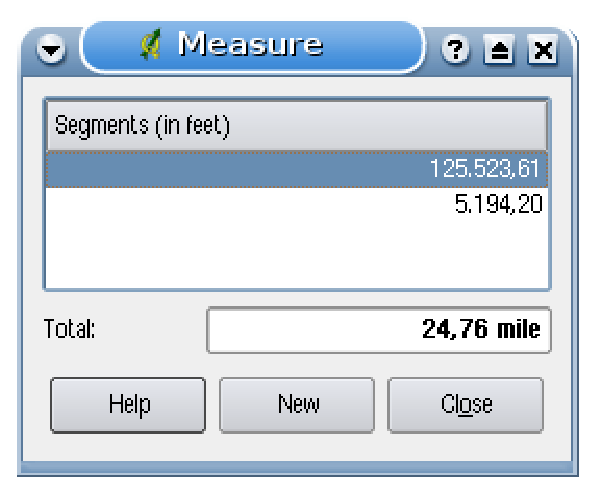
\includegraphics[clip=true, width=0.3\textwidth]{measure_line}}\goodgap
   \subfigure[Misura aree]{\label{subfig:measure_area}\includegraphics[clip=true, width=0.3\textwidth]{measure_area}}
\end{figure}

\subsection{Progetti}\label{sec:projects}\index{progetti}

Lo stato della sessione QGIS è considerata un progetto. 
È possibile lavorare su un progetto alla volta. Le impostazioni possono essere settate 
per ogni singolo progetto oppure come default per tutti i nuovi progetti (si veda la Sezione
\ref{subsec:gui_options}). Lo stato della sessione corrente può essere salvato
in un progetto usando la voce di menu \mainmenuopt{File} >
\dropmenuopttwo{mActionFileSave}{Salva progetto}
o \mainmenuopt{File} > \dropmenuopttwo{mActionFileSaveAs}{Salva progetto con
nome}.

Per caricare progetti salvati usare \mainmenuopt{File} >
\dropmenuopttwo{mActionFileOpen}{Apri progetto}
o \mainmenuopt{File} > \dropmenuopt{Apri progetti recenti}.
Se si vuole eliminare la sessione corrente e ricominciare da zero, scegliere
\mainmenuopt{File} > \dropmenuopttwo{mActionFileNew}{Nuovo progetto}.
Ognuna di queste voci di menu chiederà se si vuole salvare la sessione
corrente se sono stati effettuati cambiamenti dall'ultima volta in cui essa è
stata aperta o salvata.

Le informazioni salvate nel file di progetto includono:

\begin{itemize}
\item Layers aggiunti
\item Proprietà dei layer, inclusa la loro rappresentazione grafica
\item Proiezione usata per la vista
\item Ultima estensione della vista (scala e inquadramento)
\end{itemize}

Il file di progetto è salvato in formato XML, così che sia possibile editarlo
esternamente a QGIS con qualunque editor se se conosce la sintassi. Il formato
del file di progetto è stato modificato parecchie volte rispetto a quello
delle precedenti versioni di QGIS, di conseguenza file di progetto salvati con
precedenti versioni di QGIS potrebbero non funzionare più correttamente. Si
può essere avvertiti preventivamente di ciò selezionando dalla scheda
\tab{Generale} nel menu \mainmenuopt{Impostazioni} > \dropmenuopt{Opzioni} 
la casella di controllo \checkbox{Avvisa quando un file di progetto viene
salvato con una vecchia versione di QGIS}.


\minisec{Proprietà progetto}
Nella finestra delle proprietà del progetto (sotto \nix{\mainmenuopt{File} > \dropmenuopt{Proprietà progetto}} o \win{\mainmenuopt{Impostazioni} > \dropmenuopt{Proprietà progetto} } possono essere impostate opzioni specifiche del progetto. Queste includono:
\begin{itemize}
 \item Nella tabella \tab{Generale} il titolo del progetto, unità, e l'opzione per salvare i percorsi relativi ai layer. Qui possono essere impostate anche opzioni per l'editing topologico e per lo snapping.
\item La tabella \tab{CRS} Sistema di proiezione delle coordinate permette di scegliere il sistema di proiezione delle coordinate e di abilitare la riproiezione al volo dei layer vettoriali quando vengono visualizzati layer con differenti CRS.
\item Con la terza tabella \tab{Layer interrogabili} è possibile impostare (o disabilitare) quali layer risponderanno allo strumento di interrogazione. (Vedere il paragrafo Strumenti mappa nella sezione \ref{subsec:gui_options} per abilitare l'interrogazione di layer multipli.)
\end{itemize}

\subsection{Output}\label{sec:output}\index{output!salva come immagine!compositore stampe}
Ci sono diversi modi di generare file di output dalla sessione QGIS.
Il primo è stato descritto alla Sezione \ref{sec:projects} e consiste nel
salvataggio su file di progetto. 
Altri modi di produrre file di output sono ad esempio:
\begin{itemize}
\item L'opzione di menu \dropmenuopttwo{mActionSaveMapAsImage}{Salva come
immagine} apre una finestra del file browser nella quale indicare nome,
percorso ed estensione del formato immagine (PNG or JPG).
\item L'opzione di menu \dropmenuopttwo{mActionFilePrint}{Compositore stampe}
apre una finestra nella quale è possibile comporre un layout per stampare la
vista mappa corrente (vedi Sezione~\ref{label_printcomposer}).
\end{itemize}


\subsection{Opzioni dell'interfaccia grafica (GUI)}\label{subsec:gui_options}

\includegraphics[width=0.7cm,clip=true]{mActionOptions} 
Alcune opzioni di base per QGIS 
possono essere impostate dalla finestra \dialog{Opzioni} dialog. Selezionare la 
voce di menu \mainmenuopt{Impostazioni} >
 \dropmenuopttwo{mActionOptions}{Opzioni}. Le schede nelle quali possono
 essere regolate le opzioni sono:

\minisec{Generale}

\begin{itemize}
\item \checkbox{Suggerisci di salvare i cambiamenti di progetto se necessario}
\item \checkbox{Avvisa quando un file di progetto viene salvato con una
vecchia versione di QGIS}
\item Scelta del colore per evidenziare la selezione e lo sfondo della vista mappa
\item Cambio del tema delle icone (scelta tra default, classica, gis e nkids)
\item \checkbox{Rendi maiuscoli i nomi dei layer nella legenda}
\item \checkbox{Visualizza i nomi degli attributi della classificazione della
legenda}
\item \checkbox{Nascondi lo splash screen all'avvio}
\item \checkbox{Apri i risultati di un'interrogazione in una finestra separata (è necessario
riavviare QGIS)}
\item \checkbox{Apri la tabella attributi in una finestra separata}
\item \checkbox{Aggiungi un layer PostGIS con un doppio click e seleziona la modalità estesa}
% \item Comportamento della tabella attributi (scelta tra mostra tutte le
% geometrie, mostra le geometrie selezionate, mostra le geometrie della vista attuale)
\end{itemize}

\minisec{Disegno}

\begin{itemize}
\item \checkbox{Per impostazione predefinita i nuovi layer aggiunti alla mappa
vengono visualizzati subito}
\item Definizione del numero di geometrie da disegnare prima di aggiornare lo
schermo.
\item \checkbox{Rendi le linee meno dettagliate in favore di migliori
prestazioni di disegno}
\item \checkbox{Risolvi problemi con i poligoni riempiti non correttamente}
% \item \checkbox{Ridisegna la mappa mentre viene spostato il divisore legenda/mappa} 
\end{itemize}

\minisec{Strumenti mappa}

\begin{itemize}
\item L'impostazione Modalità determina quali layer saranno mostrati attraverso
lo strumento Identifica geometrie. Passando a \usertext{Su giù} invece di 
\usertext{Layer in uso} gli attibuti per tutti i layer selezionabili
(Si veda la sezione Proprietà progetto in: \ref{sec:projects} per impostare quali
layer siano selezionabili) saranno visibili tramite lo strumento Identifica geometrie.
\item Definizione del raggio di ricerca per identificare gli oggetti e
visualizzare le relative informazioni sulla mappa in percentuale della
larghezza della mappa
\item Definizione dell'ellissoide da impiegare per il calcolo delle distanze
\item Definizione del colore della traccia (colore elastico) nello strumento
misura
\item Definizione delle unità di misura preferite (metri o piedi)
\item Definizione del comportamento della rotellina del mouse (Zoom, Zoom e
centramento, Zoom al cursore del mouse, Niente)
\item Definizione del fattore di zoom quando si aziona la rotellina del mouse
\end{itemize}

\minisec{Sovrapposizione}

\begin{itemize}
\item Definizione dell'algoritmo di piazzamento per le etichette (scelta tra punto centrale
(standard), catena, catena tabu popmusic, tabu popmusic e catena popmusic)
\end{itemize}

\minisec{Digitalizzazione}

\begin{itemize}
\item Definizione del colore e della larghezza della traccia quando si digitalizza
\item Definizione della modalità di aggancio predefinita (al vertice, al
segmento o entrambe)
\item Definizione della tolleranza (distanza massima) per attivare lo snapping
in unità del layer
\item Definizione del raggio di ricerca per la cattura e modifica di vertici
in unità del layer
\item \checkbox{Mostra i marcatori solo per le geometrie selezionate}
\item Definizione dello stile (croce, cerchio semitrasparente o nessuno) e della
dimensione per il marcatoredei vertici 
\item \checkbox{Chiusura della finestra di pop-up degli attributi dopo la creazione
di ogni geometria}
\end{itemize}

\minisec{CRS}

\begin{itemize}
\item \checkbox{Richiesta per CRS} 
\item \checkbox{CRS predefinito utilizzato dal progetto}
\item \checkbox{Verrà utilizzato il seguente CRS globale predefinito
visualizzato qui sotto}
\item Selezioni globali predefinite
\end{itemize}

\minisec{Lingua}

\begin{itemize}
\item \checkbox{Sovrascrivi lingua in uso}
\item Informazioni sulla lingua correntemente impostata nel sistema
\end{itemize}

\minisec{Proxy}

\begin{itemize}
\item \checkbox{Utilizza un proxy per l'accesso web}, definizione di host,
porta, utente e password.
\item Definizione del \dropmenuopt{Tipo proxy} secondo le esigenze
 \begin{itemize}
  \item \dropmenuopt{Default Proxy}: Il proxy è determinato sulla base delle impostazioni in uso del proxy dell'applicazione
  \item \dropmenuopt{Socks5Proxy}: Proxy generico per ogni tipo di connessione. Supporta TCP, UDP, associazione a una porta (connessione in entrata) e autenticazione.
  \item \dropmenuopt{HttpProxy}: Realizzato usando il comando "CONNECT", supporta solamente connessioni TCP in uscita; supporta l'autenticatione.
  \item \dropmenuopt{HttpCachingProxy}: Realizzato usando normali comandi HTTP, è utile solamente nel contesto di richieste HTTP.
  \item \dropmenuopt{FtpCachingProxy}: Realizzato usando un proxy FTP, è utile solamente nel contesto di richieste FTP.
 \end{itemize}
\end{itemize}

Si possono escludere alcune URL aggiungendole nella casella di testo al di sotto delle impostazioni del proxy (vedere
fig. \ref{fig:proxy-settings}) premendo il pulsante \button{Aggiungi}. In seguito 
fare doppio click nel campo URL appena creato e inserire l'URL che si desidera
escludere dall'utilizzo del proxy. Ovviamente il pulsante \button{Rimouvi} elimina
l'elemento selezionato.

Per informazioni più dettagliate sulle diverse impostazioni del proxy,
si prega di fare riferimento al manuale della documentazione delle librerie QT su
\url{http://doc.trolltech.com/4.5/qnetworkproxy.html#ProxyType-enum}.

\begin{figure}[ht]
   \begin{center}
   \caption{Impostazioni del proxy in QGIS \nixcaption}
   \includegraphics[clip=true, width=10cm]{proxy-settings}
   \label{fig:proxy-settings}
\end{center} 
\end{figure}

\begin{Tip} \caption{\textsc{Utilizzo dei proxy}}
\qgistip{L'utilizzo dei proxy può a volte essere complicato. E' utile testare 
i tipi di proxy succitati e controllare il loro funzionamento nel vostro caso specifico.
}
\end{Tip}

Queste opzioni possono essere modificate in funzione delle specifiche
esigenze. Alcuni cambiamenti potrebbero rendere necessario riavviare QGIS
prima che divengano attivi.

\begin{itemize}
\item \nix{Le impostazioni sono salvate in un file di testo: \$HOME/.config/QuantumGIS/qgis.conf}
\item \osx{Le impostazioni vengono collocate in: \$HOME/Library/Preferences/org.qgis.qgis.plist}
\item \win{Le impostazioni vengono inserite nel registro di sistema alla voce:}
\begin{verbatim}
\\HKEY\CURRENT\USER\Software\QuantumGIS\qgis
\end{verbatim}
\end{itemize}


\subsection{Segnalibri geospaziali}\label{sec:bookmarks}
\index{segnalibri}
\index{segnalibri geospaziali|\see{segnalibri}}

I segnalibri geospaziali consentono di "memorizzare" una posizione
geografica alla quale ritornare in un secondo momento.

\subsubsection{Creazione di un segnalibro}
Per creare un segnalibro:
\begin{enumerate}
\item Usare lo zoom o muovere la mappa all'estensione d'interesse.
\item Selezionare la voce di menu \mainmenuopt{Visualizza} >
\dropmenuopt{Nuovo segnalibro} o premere \keystroke{Ctrl-B}.
\item Inserire un nome descrittivo per il segnalibro (fino a 255 caratteri).
\item Cliccare su \button{OK} per aggiungere il segnalibro o \button{Cancel}
per uscire senza aggiungere il segnalibro.
\end{enumerate}

Si noti che è possibile avere più di un segnalibro con lo stesso nome.

\subsubsection{Uso e gestione dei segnalibri}
Per usare o gestire i segnalibri, selezionare la voce di menu
\mainmenuopt{Visualizza} > \dropmenuopt{Mostra segnalibri}.
La finestra \dialog{Segnalibri geospaziali} consente di usare lo zoom a un
segnalibro o di eliminarne uno.
Non è possibile editare il nome o le coordinate di un segnalibro.

\subsubsection{Zoom a un segnalibro}
Dalla finestra \dialog{Segnalibri geospaziali} dialog, selezionare il
segnalibro desidera cliccando su di esso, quindi cliccare su \button{Zoom a}.
Si può usare lo zoom su un segnalibro anche facendo doppio click su di esso.

\subsubsection{Cancellare un segnalibro}
Per cancellare un segnalibro dalla finestra \dialog{Segnalibri geospaziali},
cliccare su di esso e poi sul pulsante \button{Elimina}.
Confermare la scelta cliccando su \button{OK} o annullare l'eliminazione
cliccando su \button{Cancel}.

% vim:autoindent:set textwidth=78:

\section{Trabajando con datos vectoriales}\label{label_workingvector}
\index{vector layers|(}

% when the revision of a section has been finalized,
% comment out the following line:
%\updatedisclaimer


QGIS suporta datos vectoriales en un n\'umero de formatos, incluyendo los formatos soportados por el proveedor de datos de la librer\'{\i}a OGR, tales como ESRI shapefiles,
\index{shapefiles}\index{ESRI!shapefiles}\index{SHP files}
MapInfo MIF (formato de intercambio)\index{MIF files}\index{MapInfo!MIF files}
y MapInfo TAB (formato nativo).\index{TAB files}\index{MapInfo!TAB files}
Puede encontrar una lista de los formatos vectoriales soportados por OGR en el Ap\'endice~\ref{appdx_ogr}.

QGIS tambien soporta capas de PostGIS\index{PostGIS}\index{PostgreSQL!PostGIS} en una base de datos PostgreSQL usando el proveedor de datos PostgreSQL. El soporte para tipos de datos adicionales (ej. texto delimitado) se provee a trav\'es de proveedores de datos adicionales.\index{delimited text}

Esta secci\'on describe como trabajar con diferentes formatos comunes:
ESRI shapefiles, capas de PostGIS, y capas de SpatialLite. Muchas de las caracter\'{\i}sticas disponibles en QGIS trabajan de la misma forma, independientemente de la fuente de datos vectoriales.
Esto es por dise\~no e incluyen las funciones de identificar, seleccionar, etiquetar y de atributos.

El c\'omo trabajar con vectores de GRASS se describe en la Secci\'on \ref{sec:grass}.

\subsection{ESRI Shapefiles}
\index{vector layers!ESRI shapefiles}
\index{shapefiles}
\index{ESRI!shapefiles}
\index{SHP files}

El formato de archivo vectorial estandar usado en QGIS es el ESRI Shapefile. El soporte se provee a trav\'es de la librer\'{\i}a OGR Simple Feature (\url{http://www.gdal.org/ogr/})
\index{OGR}. Un shapefile actualmente consiste de m\'ultiples archivos. Los siguientes tres son requeridos:
\index{shapefile!format}

\begin{itemize}
\item \filename{.shp} archivo que contiene las geometr\'{\i}as de las caracter\'{\i}sticas.
\item \filename{.dbf} archivo que contiene los atributos en formato dBase.
\item \filename{.shx} archivo de \'{\i}ndices.
\end{itemize}

Los shapefiles tambien pueden incluir un archivo con un sufijo \filename{.prj}, que contiene la informaci\'on de proyecci\'on. Mientras es muy \'util tener un archivo de proyecci\'on, no es obligatorio. Un conjunto de datos shapefile puede contener archivos adicionales. Para mayores detalles vea la especificaci\'on t\'ecnica de ESRI en  \url{http://www.esri.com/library/whitepapers/pdfs/shapefile.pdf}
\index{shapefile!specification}.

\subsubsection{Cargando un Shapefile}\label{sec:load_shapefile}

\begin{figure}[ht]
   \begin{center}
   \caption{Di\'alogo Abrir Capa Vectorial \nixcaption}\label{fig:addvectorlayer}\smallskip
   \includegraphics[clip=true, width=12cm]{addvectorlayerdialog}
\end{center} 
\end{figure}

\begin{figure}[ht]
   \begin{center}
   \caption{Di\'alogo Abrir una Capa Vectorial de OGR \nixcaption}\label{fig:openshapefile}\smallskip
   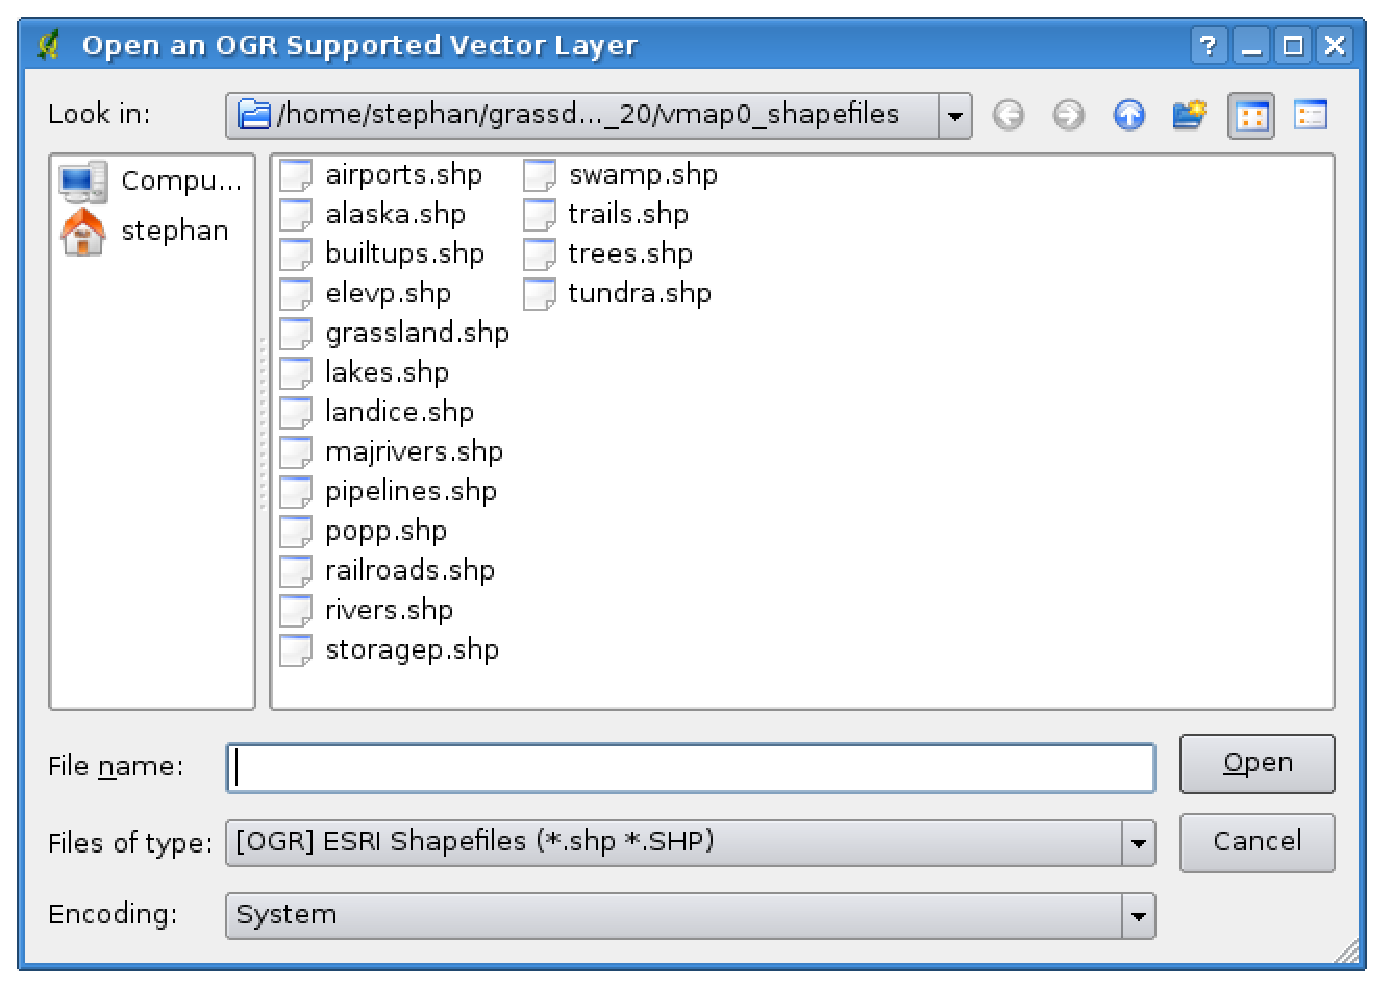
\includegraphics[clip=true, width=14cm]{shapefileopendialog}
\end{center} 
\end{figure}

\begin{figure}[ht]
   \begin{center}
   \caption{QGIS con un shapefile de Alaska cargado \nixcaption}\label{fig:loadedshapefile}\smallskip
   \includegraphics[clip=true, width=16cm]{shapefileloaded}
\end{center} 
\end{figure}

\includegraphics[width=0.7cm]{mActionAddNonDbLayer} Para cargar un shapefile, inicie
QGIS y haga clic en el bot\'on \toolbtntwo{mActionAddNonDbLayer} de la barra de herramientas{A\~nadir una capa vectorial}
\index{shapefile!loading} o simplemente presione la tecla \keystroke{V}. Esto abrir\'a una nueva ventana (vea la Figura \ref{fig:addvectorlayer}).  

De los botones de selecci\'on disponibles verifique \radiobuttonon{Archivo}. Clic en \button{Explorar}. Eso traer\'a un di\'alogo de abrir archivo estandar (vea la Figura \ref{fig:openshapefile}) que permite navegar el sistema de archivos y cargar un  shapefile o cualquier otra fuente de datos soportada. 
La caja de selecci\'on \selectstring{Ficheros de tipo}{\ldots} permite preseleccionar algunos formatos de archivos OGR soportados.

Puede seleccionar tambien el tipo de codificaci\'on deseado para el shapefile.

Seleccionando un shapefile de la lista y haciendo clic en \button{Abrir} lo carga dentro de QGIS. La Figura
\ref{fig:loadedshapefile} muestra QGIS despues de cargar el archivo \filename{alaska.shp}.


\begin{Tip}\caption{\textsc{Colores de la capa}}
\qgistip{Cuando agrega una capa al mapa, se le asigna un color de manera aleatoria. Cuando se
agrega mas de una capa al mismo tiempo, se le asigna diferentes colores a cada capa. }
\end{Tip}

Una vez cargado, puede hacer acercamientos o alejamientos al shapefile usando las herramientas de navegaci\'on del mapa.
Para cambiar la simbolog\'ia de la capa, abra el di\'alogo \dialog{Propiedades de la capa} haciendo doble clic en el nombre de la capa o haciendo clic derecho en el nombre de la capa en la leyenda y eligiendo \dropmenuopt{Propiedades} del men\'u emergente. Vea la  Secci\'on \ref{sec:symbology} para mas informaci\'on sobre como configurar la simbolog\'{\i}a para capas vectoriales.
  
\subsubsection{Mejorando el rendimiento}

Para mejorar el rendimiento del dibujado de un shapefile, puede crear un \'{\i}ndice espacial. Un \'{\i}ndice espacial \index{spatial index!shapefiles} mejorar\'a la velocidad en las operaciones de acercar, alejar y desplazar. Los \'{\i}ndices espaciales usados por QGIS tienen una extensi\'on \filename{.qix}.

Use estos pasos para crear el \'{\i}ndice:

\begin{itemize}
\item Cargue un shapefile.
\item Abra el di\'alogo \dialog{Propiedades de la capa} haciendo doble clic en el nombre del shapefile en la leyenda o haciendo clic derecho en el nombre de la capa en la leyenda y eligiendo \dropmenuopt{Propiedades} del men\'u emergente.
\item En la pesta\~na general \tab{General} haga clic en el bot\'on \button{Crear \'Indice Espacial}.
\end{itemize}

\subsubsection{Cargando una capa de MapInfo}
\index{vector layers!MapInfo}

Para cargar una capa de MapInfo, haga clic en el bot\'on  \toolbtntwo{mActionAddNonDbLayer}{A\~nadir capa vectorial}
de la barra de herramientas o presione la tecla \keystroke{V}, cambie el filtro de tipo de archivo a
\selectstring{Ficheros de tipo}{[OGR] MapInfo (*.mif
*.tab *.MIF *.TAB)} y seleccione la capa que desea cargar.

\subsubsection{Cargando un ArcInfo Binary Coverage}
\index{vector layers!ArcInfo Binary Coverage}

Para cargar un ArcInfo binary coverage haga clic en el bot\'on  
\toolbtntwo{mActionAddNonDbLayer}{A\~nadir capa vectorial} de la barra de herramientas
o presione la tecla \keystroke{V} para abrir el di\'alogo 
\dialog{A\~nadir capa vectorial}.  Seleccione \radiobuttonon{Directorio}. Cambie a \selectstring {Tipo}{Arc/Ingo Binary Coverage}. 
Navegue al directorio que contiene los archivos de coberturas y selecci\'onelo.

Similarmente, puede cargar vectores basados en directorio como el formato UK National Transfer as\'{\i} como el 
formato raw TIGER del US Census Bureau.

\subsection{Capas PostGIS}
\index{vector layers!PostGIS|see{PostGIS}}
\index{PostGIS!layers}
\label{label_postgis} 

Las capas de PostGIS son almacenadas en una base de datos PostgreSQL. Las ventajas de PostGIS
son indexamiento espacial, filtrado y las capacidades de consulta que provee. Usando POstgis, funciones
vectoriales tales como seleccionar e identificar funcionan mucho mas eficazmente que con
capas OGR en QGIS.

Para usar capas de PostGIS debe de:\index{PostgreSQL!loading layers}
\begin{itemize}
\item Crear una conexi\'on almacenada en QGIS a la base de datos PostgreSQL (si no ha sido
previamente definida).\index{PostgreSQL!connection}
\item Conectarse a la base de datos.
\item Seleccionar la capa a agregar al mapa.
\item Opcionalmente proveer una clausula SQL \usertext{where}
para definir que caracter\'{\i}sticas cargar desde la capa.
\item Cargar la capa.
\end{itemize}

\subsubsection{Creando una conexi\'on almacenada}\index{PostgreSQL!connection}\label{sec:postgis_stored}


\includegraphics[width=0.7cm]{mActionAddLayer} La primera vez que utilize un conjunto de datos PostGIS, debe crear una conexi\'on a la base de datos PostgreSQL que contiene los datos. Comienze haciendo clic en el bot\'on \toolbtntwo{mActionAddLayer}{A\~nadir capa de PostGIS} de la barra de herramientas, seleccionando la opci\'on 
\dropmenuopttwo{mActionAddLayer}{A\~nadir capa de PostGIS...} del men\'u \mainmenuopt{Capa} o presionando la tecla \keystroke{D}. Tambien puede abrir el di\'alogo \dialog{A\~nadir capa vectorial} y seleccionar \radiobuttonon{Base de datos}.
Se abrir\'a el di\'alogo \dialog{A\~nadir tabla(s) PostGIS}. Para accesar al manejador de conexiones \index{PostgreSQL!connectionmanager}, haga clic en el bot\'on \button{Nueva} para mostrar el di\'alogo  \dialog{Crear una nueva conexi\'on a PostGIS}. Los par\'ametros requeridos para una conexi\'on se muestran en la tabla \ref{tab:postgis_connection_parms}.

\begin{table}[ht]\index{PostgreSQL!connection parameters}
\centering
\caption{Par\'ametros de conexi\'on a PostGIS}\label{tab:postgis_connection_parms}\medskip
 \begin{tabular}{|l|p{5in}|}
\hline Nombre & Un nombre para esta conexi\'on. Puede ser la misma que \textsl{Base de datos}.
\\
\hline Servidor \index{PostgreSQL!host}
& Nombre del servidor de bases de datos. Este debe ser un nombre de servidor que pueda ser resuelto como puediera
ser usado para abrir una conexi\'on telnet o hacer un ping al servidor. Si la base de datos est\'a 
en la misma computadora que QGIS, simplemente introdusca 'localhost' aqu\'{\i}. \\
\hline Base de datos \index{PostgreSQL!database} & Nombre de la base de datos.  \\
\hline Puerto \index{PostgreSQL!port}& N\'umero del puerto en el que el servidor 
de base de datos PostgreSQL escucha. El puerto por defecto es el 5432.\\
\hline Nombre de Usuario \index{PostgreSQL!username}& El nombre de usuario es usado para iniciar sesi\'on
a la base de datos. \\
\hline Contrase\~na \index{PostgreSQL!password}& Contrase\~na usada para
\textsl{Nombre de usuario} conectarse a la base de datos.\\
\hline Modo SSL \index{PostgreSQL!sslmode}& Como ser\'a negociada la conexi\'on SSL con el servidor. Estas son las opciones: 
\begin {itemize}
\item desactivar: solo tratar una conexi\'on SSL no encriptada;
\item permitir: tratar una conexi\'on sin SSL, si falla, intentar una conexi\'on SSL;
\item preferir (predeterminada): intentar una conexi\'on SSL, si falla, intentar una conexi\'on no-SSL;
\item requerir: solo intentar una conexi\'on SSL.
\end {itemize}
Note se puede alcanzar aumentos masivos en la velocidad de presentado de capas PostGIS desactivando SSL en el editor de conexiones. \\
\hline
\end{tabular}
\end{table}

Opcionalmente puede activar las siguientes casillas:

\begin{itemize}
\item \checkbox{Guardar contrase\~na}
\item \checkbox{Solo buscar en la tabla geometry\_columns}
\item \checkbox{Solo buscar en el esquema 'public'}
\end{itemize}

Una vez que todos los par\'ametros y opciones son establecidos, puede probar la conexi\'on haciendo clic 
en el bot\'on \button{Probar Conexi\'on} \index{PostgreSQL!connection!testing}.

\begin{Tip}\caption{\textsc{Configuraciones de Usuario y Seguridad de QGIS}}\index{settings}\index{security}
\qgistip{Sus configuraciones personalizadas para QGIS son almacenadas en el sistema
operativo. En \nix, las configuraciones son almacenadas en su directorio home en
\filename{.qt/qgisrc}. En \win, las configuraciones son almacenadas en el registro. Dependiendo de su
ambiente de computo, almacenar contrase\~nas en sus configuraciones de QGIS puede ser
un riesgo de seguridad.
}
\end{Tip}

\subsubsection{Cargando una capa PostGIS}\index{PostgreSQL!loading layers}


\includegraphics[width=0.7cm]{mActionAddLayer} Una vez que tiene una o mas
conexiones definidas, puede cargar capas desde la base de datos PostgreSQL. Claro
que esto requiere tener datos en PostgreSQL. Vea la secci\'on
\ref{sec:loading_postgis_data} para una discusi\'on sobre importar datos dentro de la
base de datos. 

Para cargar una capa de PostGIS, realize los siguientes pasos:

\begin{itemize}
\item Si el di\'alogo \dialog{A\~nadir tabla(s) PostGIS} no esta abierto aun, haga clic en el bot\'on
\toolbtntwo{mActionAddLayer}{A\~nadir Capa PostGIS}de la barra de herramientas.
\item Elija la conexi\'on de la lista desplegable y haga clic en \button{Connectar}.
\item Encuentre la capa que desea agregar en la lista de capas disponibles.
\item Seleccionela haciendo clic en ella. Puede seleccionar m\'ultiples capas presionando
la tecla \keystroke{shift} mientras hace clic. Vea la secci\'on \ref{sec:query_builder} para
informaci\'on sobre usar el Constructor de Consultas de PostgreSQL para definir con mas precisi\'on la capa.
\item Clic en el bot\'on \button{A\~nadir} para agregar una capa al mapa.
\end{itemize}

\begin{Tip}\caption{\textsc{Capas PostGIS}}
\qgistip{Normalmente una capa PostGIS es definida por una entrada en la tabla
geometry\_columns. Desde la versi\'on \OLD % should be 0.9.0 
hacia arriba, QGIS puede cargar capas que no tienen una entrada
en la tabla geometry\_columns. Esto incluye tablas y vistas.
La definici\'on de una vista espacial provee poderosos medios para visualizar sus datos. Rem\'{\i}tase
a su manual de PostgreSQL para informaci\'on sobre creaci\'on de vistas.}
\end{Tip}

\subsubsection{Algunos detalles acerca de capas PostgreSQL}\label{sec:postgis_details}
\index{PostgreSQL!layer details}

Esta secci\'on contiene algunos detalles de como QGIS accesa capas PostgreSQL. La mayor\'{\i}a de las veces QGIS deber\'{\i}a simplemente proveerle una lista de tablas de la base de datos que puede ser cargadas, y cargarlas cuando sea necesario. Sin embargo, si tiene problemas cargando una tabla PostgreSQL en QGIS, la siguiente informaci\'on puede ayudarle a entender cualquier mensaje de QGIS y guiarlo para cambiar la definici\'on de tabla o vista de PostgreSQL para que QGIS pueda cargarla.

QGIS requiere que las copas de PostgreSQL contengan una columna que pueda ser usada como llave \'unica para la capa. Para tablas esto usualmente significa que la tabla necesita una llave primaria, o una columna con una restricci\'on de \'unica en ella. En QGIS, esta columna necesita ser del tipo int4 (un entero de tama\~no de 4 bytes). Alternativamente una columna ctid puede ser usada como llave primaria. Si la tabla carece de estos elementos, la columna oid ser\'a usada. El rendimiento se mejorar\'a si la columna es indexada (note que las llaves primarias son indexadas autom\'aticamente en PostgreSQL). 

Si la capa PostgreSQL es una vista, existe el mismo requerimiento, pero las vistas no tienen llave primaria o columnas restricciones de valores \'unicos. En este caso QGIS tratar\'a de encontrar una columna en la vista que sea derivada de una columna adecuada. La determinaci\'on de la columna se hace analizando la definici\'on SQL de la vista. Sin embargo hay varios aspectos de SQL que QGIS ignora - estos incluyen el uso de alias en tablas y columnas que son generados por funciones SQL.

Si no es posible encontrar una columna adecuada, QGIS no cargar\'a la capa. Si esto ocurre, la soluci\'on es alterar la vista de manera que incluya una columna adecuada (de un tipo int4 y que bien sea una llave primaria o que tenga una restricci\'on de valores \'unicos en la columna, preferentement indexada). 

Cuando QGIS trabaja con vistas, analiza la definici\'on de la vista y 

\subsubsection{Importando datos a PostgreSQL}\label{sec:loading_postgis_data} \index{PostGIS!SPIT!importing data} \minisec{shp2pgsql}
Los datos pueden ser importados a PostgreSQL usando un n\'umero de m\'etodos. PostGIS
incluye una utiler\'{\i} llamada \filename{shp2pgsql} que puede ser usada para importar shapefiles a una base de datos PostgreSQL con PostGIS activado. Por ejemplo para importar un shapefile llamado \filename{lakes.shp} a una base de datos PostgreSQL llamada \usertext{gis\_data}, use el siguiente comando:

\begin{verbatim} 
  shp2pgsql -s 2964 lakes.shp lakes_new | psql gis_data
\end{verbatim}

Esto crea una capa llamada \usertext{lakes\_new} en la base de datos \usertext{gis\_data}. La nueva capa tendr\'a un identificador del sitema espacial de referencia (SRID) de 2964. Vea la secci\'on \ref{label_projections} para mas informaci\'on de sistemas de referencia espaciales y proyecciones.

\begin{Tip}
\caption{\textsc{Exporting datasets from PostGIS}\index{PostGIS!Exporting}}
\qgistip{Al igual que la herramienta de importaci\'on \filename{shp2pgsql} hay tambien una herramienta para exportar
conjuntos de datos PostGIS a shapefiles: \filename{pgsql2shp}. Esta se encuentra en 
su distribuci\'on PostGIS.} 
\end{Tip}

\minisec{SPIT Plugin}

\includegraphics[width=0.7cm]{spiticon} QGIS viene con un complemento llamado 
SPIT (Shapefile to PostGIS Import Tool)\index{PostGIS!SPIT}.
SPIT puede ser usado para cargar m\'ultiples shapefiles al mismo tiempo e inluye soporte para esquemas. Para usar SPIT, habra el Manejador de Complementos del men\'u \mainmenuopt{Plugins}, verifique la caja siguiente al \checkbox{SPIT plugin} y haga clic en el bot\'on \button{OK}. El \'{\i}cono de SPIT ser\'a agregado a la barra de herramientas de complementos \index{PostGIS!SPIT!loading}. 

Para importar un shapefile, haga clic en \'{\i}cono de la barra de herramientas \toolbtntwo{spiticon}{SPIT} para abrir el di\'alogo \dialog{SPIT - Shapefile to PostGIS Import Tool}. Seleccione la base de datos PostGIS a la que desea conectarse y haga clic en el bot\'on \button{Connect}. Ahora puede agregar uno o mas archivos a la cola haciendo clic en el bot\'on   \button{Add}. Para procesar los archivos, haga clic en el bot\'on  
\button{OK}. El progreso de la importaci\'on as\'{i} como cualquier error\\advertencia ser\'a mostrado conforme cada shapefile sea procesado.

\begin{Tip}\caption{\textsc{Importing Shapefiles Containing
PostgreSQL Reserved Words}}\index{PostGIS!SPIT!reserved words}
\qgistip{ Si es agregado un shapefile que contenga campos que sean palabras reservadas en el PostgreSQL se abrir\'a un di\'alogo mostrando el estado de cada campo. Los nombres de los campos pueden ser editados\index{PostGIS!SPIT!editing field names} antes de importarr y cambiar cualquier palabra reservada ( o cualquier otro nombre de campos que se desee). Intentar importar un shapefile con palabras reservadas como nombres de campos fallar\'a.}
\end{Tip} 

\minisec{ogr2ogr}
Ademas de \filename{shp2pgsql} y \filename{SPIT} hay otra herramienta para alimentar datos espaciales al PostGIS: \filename{ogr2ogr}. Esta herramienta es parte de la instalaci\'on de GDAL.
Para importar un shapefile a PostGIS, haga lo siguiente:
\begin{verbatim}
  ogr2ogr -f "PostgreSQL" PG:"dbname=postgis host=myhost.de user=postgres \
  password=topsecret" alaska.shp
\end{verbatim}

Esto importar\'a un shapefile  llamado \filename{alaska.shp} dentro de la base de datos PostGIS
\usertext{postgis}
usando el usuario \usertext{postgres} con ls contrase\~na \usertext{topsecret} en el servidor
\server{myhost.de}.

Note que OGR debe ser compilado con PostgreSQL para soportar PostGIS.
Esto se puede ver escribiendo
\begin{verbatim}
ogrinfo --formats | grep -i post
\end{verbatim}

Si desea utilizar comandos de PostgreSQL \filename{COPY}- en lugar del default
\filename{INSERT INTO} puede exportar la siguiente variable de ambiente( al menos disponible en \nix y \osx):
\begin{verbatim}
  export PG_USE_COPY=YES
\end{verbatim}

\filename{ogr2ogr} no crea \'{\i}ndices espaciales por defecto como lo hace \filename{shp2pgsl}. Necesita crearlos manualmente usando el comando SQL \filename{CREATE INDEX} despues como una paso extra (como se describe en la siguiente secci\'on \ref{label_improve}).

\subsubsection{Mejorando el rendimiento} \label{label_improve}

Recuperar caracter\'{\i}sticas de una base de datos PostgreSQL puede ser tardado, especialmente si se trabaja en red. Se puede mejorar el rendimiento del dibujado de capas PostgreSQL asegurando que exista un \'{\i}ndice espacial \index{PostGIS!spatial index} en cada capa de la base de datos. PostGIS suporta la creaci\'on de \'{\i}ndices GiST (Generalized Search Tree) \index{PostGIS!spatial index!GiST} para agilizar consultas espaciales de los datos.

La sintaxis para crear un \'{\i}ndice GiST\footnote{La informaci\'on de \'{\i}ndices GiST es tomada de la documentaci\'on de PostGIS
disponible en \url{http://postgis.refractions.net}}
es:

\begin{verbatim}
    CREATE INDEX [indexname] ON [tablename] 
      USING GIST ( [geometryfield] GIST_GEOMETRY_OPS );
\end{verbatim}

Note que para tablas grandes, la creaci\'on de un \'{\i}ndice puede tomar mucho tiempo. Una vez
el \'{\i}ndice es creado, debe realizarse un \usertext{VACUUM ANALYZE}. Vea la documentaci\'on de
PostGIS \cite{PostGISweb} para mas informaci\'on.

El siguiente es un ejemplo de la creaci\'on de un \'{\i}ndice GiST:
\begin{verbatim}
gsherman@madison:~/current$ psql gis_data
Welcome to psql 8.3.0, the PostgreSQL interactive terminal.

Type:  \copyright for distribution terms
        \h for help with SQL commands
        \? for help with psql commands
        \g or terminate with semicolon to execute query
        \q to quit

gis_data=# CREATE INDEX sidx_alaska_lakes ON alaska_lakes
gis_data-# USING GIST (the_geom GIST_GEOMETRY_OPS);
CREATE INDEX
gis_data=# VACUUM ANALYZE alaska_lakes;
VACUUM
gis_data=# \q
gsherman@madison:~/current$
\end{verbatim}

\subsection{Capas SpatiaLite} 
\index{SpatiaLite layers!properties dialog}
\index{vector layers!SpatlaLIte|see{SpatiaLite}}
\index{SpatiaLite!layers}
\label{label_spatialite} 

\includegraphics[width=0.7cm]{mActionAddSpatiaLiteLayer}
Para cargar datos desde una base de datos Spatialite, comienze haciendo clic en el bot\'on de la barra 
de herramientas \toolbtntwo{mActionAddSpatiaLiteLayer}{Add SpatiaLite Layer} o seleccionando la opci\'on  
\dropmenuopttwo{mActionAddSpatiaLiteLayer}{Add SpatiaLite Layer...} 
\mainmenuopt{Layer} del men\'u o tecleando \keystroke{L}. 
Esto mostrar\'a una ventana, la cual permitir\'a que se conecte a una base de datos Spatialite conocida por QGIS, la cual 
puede ser seleccionada del men\'u desplegable o definir una nueva conecci\'on a una base de datos. Para definir una nueva conecci\'on, haga clic en \button{New} y use el bavegador de archivos para apuntar hacia su base de datos SpatiaLite, 
el cual es un archivo con una extensi\'on \filename{.sqlite }.

\subsection{El di\'alogo de propiedades de vectores}\label{sec:vectorprops}
\index{vector layers!properties dialog}

El di\'alogo \dialog{Layer Properties} para una capa vectorial 
provee informaci\'on acerca de la capa, configuraciones
de simbolog\'{\i} y opciones de etiquetado. Si la capa vectorial ha sido cargada desde
un almacen de datos PostgreSQL / PostGIS, tambien puede alterar el SQL subyacente para la
capa - bien manualmente editando el SQL en la pesta\~na \tab{General} o invocando
el di\'alogo \dialog{Query Builder} en la pesta\~na \tab{General}. 
Para accesar al di\'alogo
\dialog{Layer Properties}, haga doble clic en un capa en la leyenda o clic derecho sobre
la capa y seleccionela del men\'u emergente \dropmenuopt{Properties}.

\begin{figure}[H]
   \begin{center}
   \caption{Di\'alogo de Propiedades de Capas Vectoriales \nixcaption}\label{fig:vector_symbology}\smallskip
   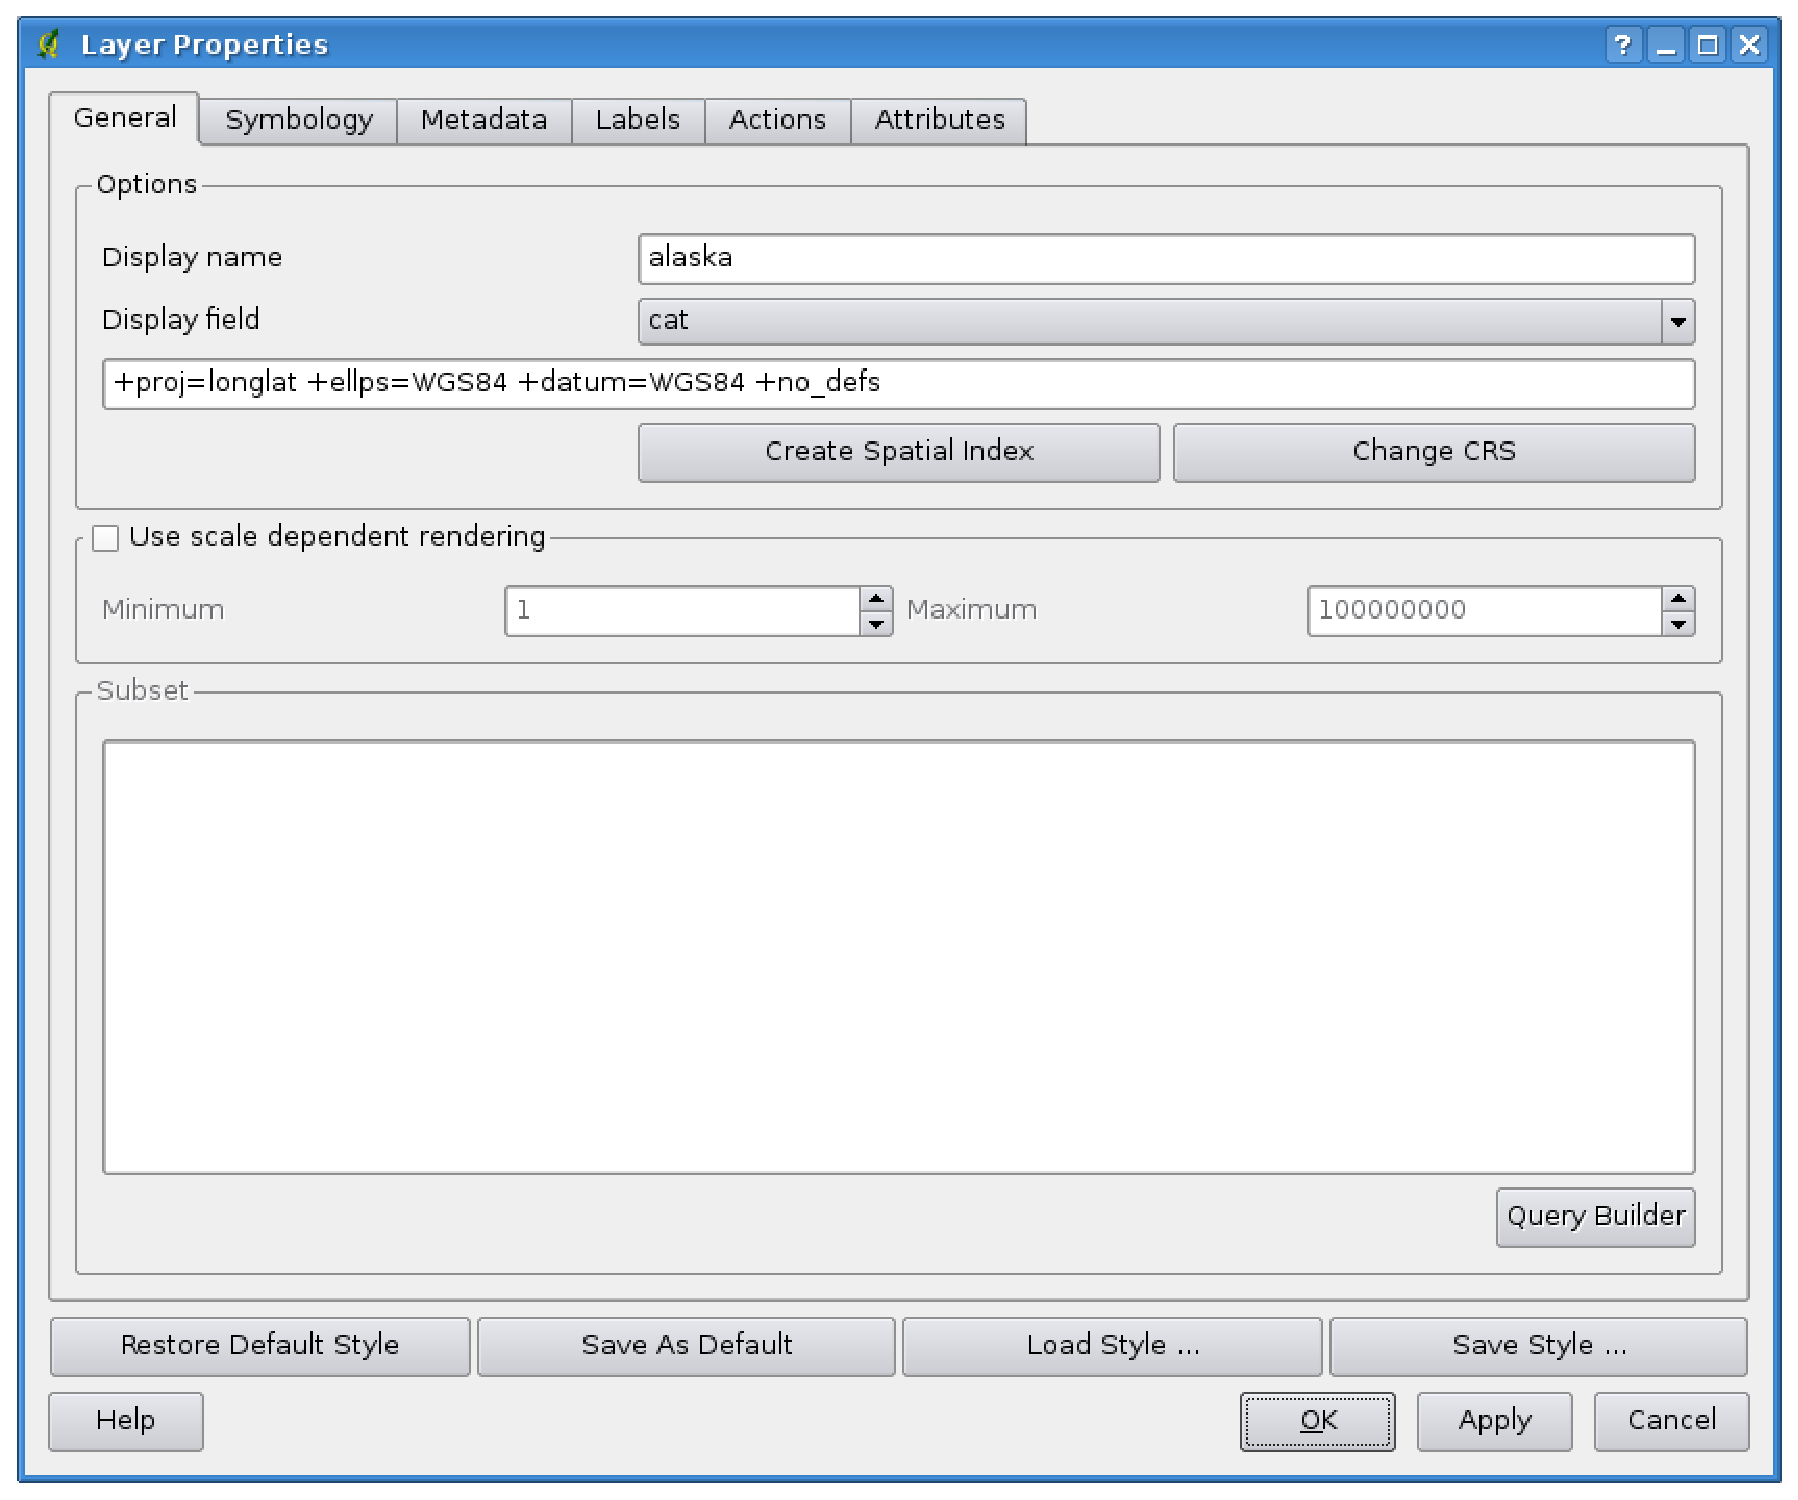
\includegraphics[clip=true, width=12cm]{vectorLayerSymbology} 
\end{center}  
\end{figure}

\subsubsection{Pesta\~na general}\label{vectorgeneraltab}
La pesta\~na \tab{General} es esencialmente muy parecida a la del di\'alogo raster. Permite
cambiar el nombre a mostrar, establecer las opciones de dibujado dependientes de la escala, crear un \'{\i}ndice espacial 
de el archivo vectorial (solo para formatos OGR y PostGIS) y ver o cambiar
la proyecci\'on espec\'{\i}fica para la capa vectorial.

El bot\'on \button{Query Builder} permite crear un subconjunto de caracter\'{\i}sticas 
en la capa - pero este bot\'on actualmente solo est\'a disponible cuando se abre la tabla  
de atributos y se selecciona el bot\'on \button{...} siguiente a b\'usqueda avanzada.

\subsubsection{Pesta\~na simbolog\'{\i} Tab}\label{sec:symbology}
\index{vector layers!symbology}

QGIS soporta un n\'umero de renderers simbolog\'{\i}as para controlar como
los caracter\'{\i}sticas vectoriales son mostradas. Actualmente los siguientes renderers
est\'an disponibles:

\begin{description} 
    \item[S\'{\i}mbolo simple] - un solo estilo es aplicado a
    cada objeto en la capa.\index{vector layers!renderers!single symbol}
    \item[S\'{\i}mbolo graduado] - los objetos dentro de la capa son
    mostrados con diferentes s\'{\i}mbolos clasificados por los valores de un
    campo particular. \index{vector layers!renderers!graduated symbol}
    \item[Color cont\'{\i}nuo] - los objetos dentro de la capa son
    mostrados con una propagaci\'on de colores clasificado por los valores
    n\'umericos de un campo espec\'{\i}fico.\index{vector layers!renderers!continuous
color}
    \item[Valor \'unico] - los objetos son clasificados por los valores \'unicos
    dentro de un campo especificado teniendo cada valor un diferente s\'{\i}mbolo.
    \index{vector layers!renderers!unique value}
\end{description}

Para cambiar la simbolog\'{\i}a de una capa, simplemente has doble clic en su entrada
en la leyenda y el di\'alogo de propiedades del vector \dialog{Layer Properties} se mostrar\'a.\index{symbology!changing}

\begin{figure}[h]
\centering
\caption{Symbolizing-options \nixcaption}
   \subfigure[S\'{\i}mbolo simple] {\label{subfig:single_symbol}\includegraphics[clip=true, width=0.4\textwidth]{vectorClassifySingle}}\goodgap
   \subfigure[S\'{\i}mbolo graduado] {\label{subfig:graduated_symbol}\includegraphics[clip=true, width=0.4\textwidth]{vectorClassifyGraduated}}\\
   \subfigure[Color cont\'{\i}nuo] {\label{subfig:cont_color}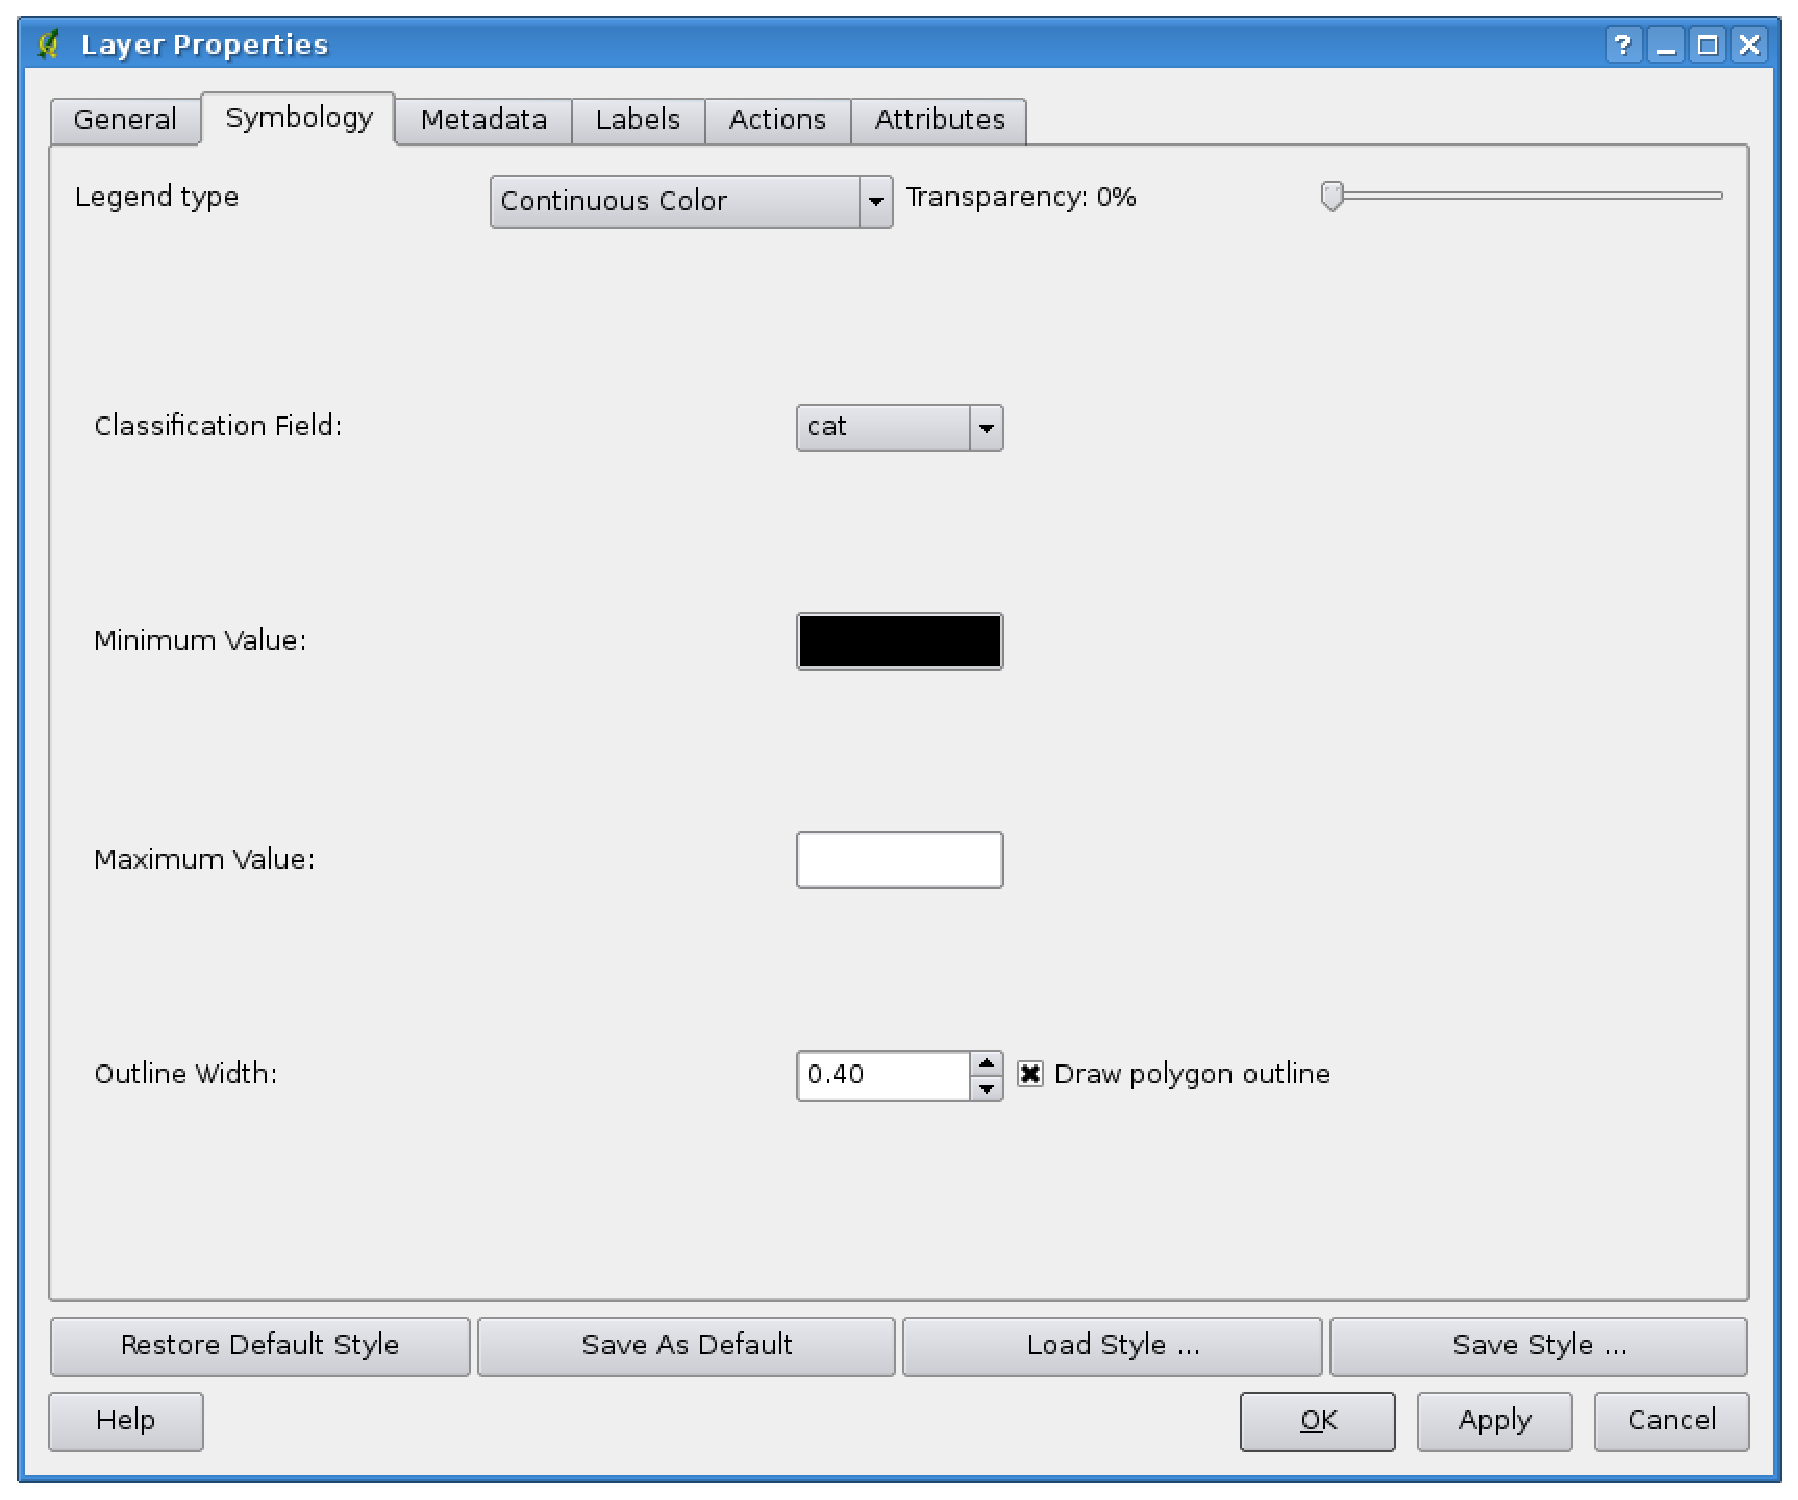
\includegraphics[clip=true, width=0.4\textwidth]{vectorClassifyContinous}}\goodgap
   \subfigure[Valor \'unico] {\label{subfig:unique_val}\includegraphics[clip=true, width=0.4\textwidth]{vectorClassifyUnique}}
\end{figure}

% FIXME: outdated
% Since \usertext{version v0.9} there is a function to use image files stored on 
% your computer as fill pattern for vector layers.

\minisec{Style Options} \label{sec:style_options} \index{vector layers!styles}
Dentro de este di\'alogo se puede definir el estilo de la capa vectorial. Dependiendo de la opci\'on
seleccionada de dibujado tambien es posible clasificar caracter\'{\i}sticas del mapa.

Al menos las siguientes opciones de estilo pueden aplicarse para casi todos los renderers:
\begin{description}
 \item[Estilo de borde] - estilo de lapiz para el borde de las caracter\'{\i}sticas. Tambien puede ser
 establecido a 'sin lapiz'.
 \item[Color de borde] - color del borde de las caracter\'{\i}sticas.
 \item[Ancho de borde] - ancho del borde de las caracter\'{\i}sticas.
 \item[Color de relleno] - color de relleno de las caracter\'{\i}sticas.
 \item[Estilo de relleno] - estilo para el relleno. Aparte de las brochas definidas puede
 seleccionar \selectstring{Fill style}{? texture} y hacer clic en el bot\'on \browsebutton
 para seleccionar su propio estilo de relleno. Actualmente los formatos soportados son
 \filename{*.jpeg, *.xpm, and *.png}.
\end{description}

Una vez que ha estilizado su capa tambien puede almacenar su estilo de capa a
un archivo separado (con extensi\'on \filename{*.qml}).
Para hacer esto, use el bot\'on \button{Save Style \ldots}. No hay necesidad de decir que
\button{Load Style \ldots} carga el archivo de estilo previamente almacenado.

Si se desea siempre usar un estilo particular siempre que la capa es cargada, 
use el bot\'on \button{Save As Default} para hacer su estilo el estilo por defecto. Tambien, 
si hace cambios al estilo y no esta contento con los cambios, use el bot\'on \button{Restore 
Default Styel} para revertir a su estilo por defecto.

\minisec{Transparencia de vectores} \label{sec:vect_transparency} \index{vector layers!transparency}
QGIS \CURRENT soporta el establecer transparencia para cada capa vectorial. Esto puede ser hecho con
la barra de desplazamiento \slider{Transparency}{0}{20mm} dentro de la pesta\~na \tab{symbology} (vea la fig. \ref{fig:vector_symbology}).
Esto es muy \'util para sobreponer varias capas vectoriales.

\subsubsection{Pesta\~na metadatos}

La pesta\~na \tab{Metadata} contiene informaci\'on acerca de la capa, incluyendo peculiaridades
acerca del tipo y localizaci\'on, n\'umero de caracter\'{\i}sticas, tipo de caracter\'{\i}stica, y las capacidades de edici\'on.
La Secci\'on \guiheading{Layer Spatial Reference System}, provee 
informaci\'on de proyecci\'on, y la secci\'on \guiheading{Attribute field info},
lista los campos y sus tipos de datos. Esta es una forma r\'apida de obtener informaci\'on acerca de la capa.

\subsubsection{Pesta\~na etiquetas}

La pesta\~na \tab{Labels} permite activar el etiquetado de caracter\'{\i}sticas y controlar un n\'umero de opciones
relacionadas con las fuentes, colocaci\'on, estilo, alineaci\'on y buffering.

Vamos a ilustrar esto etiquetando el shapefile lakes de el 
\filename{qgis\_example\_dataset}:

\begin{enumerate}
\item Cargar el shapefile \filename{alaska.shp} y el archivo GML \filename{lakes.gml} en QGIS.
\item Acerquese un poco a su area favorita con alg\'un lago.
\item Haga la capa \filename{lakes} la capa activa.
\item Abra el di\'alogo \dialog{Layer Properties}.
\item Clic en la pesta\~na \tab{Labels}.
\item Verifique la caja de selecci\'on \checkbox{Display labels} para activar el etiquetado.
\item Elija el campo a usar en el etiquetado. 
  Usaremos \selectstring{Field containing label}{NAMES}.
\item Escriba un valor por defecto para lagos que no tengan nombre. La etiqueta por defecto ser\'a
  usada cada vez que QGIS encuentre un lago sin valor en el campo \guilabel{NAMES}.
\item Si tiene etiquetas que se extienden sobre varia l\'{\i}neas, verifique \checkbox{Multiline labels?}. 
QGIS verificar\'a una verdadera l\'{\i}nea sea regresada en su campo etiqueta e inserta retornos de l\'{\i}nea como corresponda.
Una verdadera l\'{\i}nea regresada es un caracter \textbf{single} \textbackslash n, 
(no dos caracteres separados, como una diagonal invertida \textbackslash ~seguida del caracter n).
\item clic en el bot\'on \button{Apply}.
\end{enumerate} 

Ahora tenemos etiquetas. Como se ven? Probablemente muy grander y pobremente colocadas en relaci\'on al s\'{\i}mbolo
marcador para los lagos.

Seleccione la entrada \tab{Font} y use los botones  \button{Font} y \button{Color}
para establecer la fuente y el color. Tambien puede cambiar el \'angulo y la posici\'on de la etiqueta de texto.


Para cambiar la posici\'on del texto relativo a la caracter\'{\i}stica:

\begin{enumerate} 
\item Hacen clic en la entrada \tab{Font}.
\item Cambiar el posicionamiento seleccionando uno de los botones de selecci\'on
en el grupo \classname{Placement}. Para fijar las etiquetas, elija el bot\'on de selecci\'on
\radiobuttonon{Right}.
\item el \classname{Font size units} permite seleccionar entre
\radiobuttonon{Points} o \radiobuttonon{Map units}.
\item Haga clic \button{Apply} para ver los cambios sin cerrar el di\'alogo.
\end{enumerate} 

Las cosas se ven mejor, pero las etiquetas est\'an aun muy cerca del marcador. Para
arreglar esto podemos usar las opciones en la entrada \tab{Position}. Aqu\'{\i} podemos agregar 
desplazamientos en las direcciones X y Y. Agregando un desplazamiento de 5 mover\'a las etiquetas
fuera del marcador y las har\'a mas legibles. Claro esto si el s\'{i}mbolo marcador
o la fuente es muy grande, ser\'a necesario un desplazamiento mayor.

El \'ultimo ajuste que haremos es \tab{buffer} las etiqueta. Esto significa
poner un fondo alrededor de ellas para que se vean mejor. Para hacer un buffer a las
etiquetas de lagos:

\begin{enumerate}
\item Clic en la pesta\~na \tab{Buffer}.
\item Clic en la casilla de verificaci\'on  \checkbox{Buffer Labels?} para activar el buffering.
\item Elija el tama\~no del buffer usando el spin box.
\item Elija un color haciendo clic en \button{Color} y eligiendo el color favorito
  con el selector de colores. Puede establecer alguna transparencia para el buffer
  si lo prefiere.
\item Clic \button{Apply} para ver si los cambios le agradan.
\end{enumerate} 

Si no est\'as feliz con los resultados, afine las configuraciones y pruebe nuevamente
haciendo clic en \button{Apply}.

Un buffer de un 1 punto parece dar un buen resultado.
Note que puede tambien especificar un tama\~no de buffer en unidades de mapa si eso trabaja mejor
para usted.

Las entradas restantes en la pestan\~a \tab{Label} permiten controlar la apariencia de las
etiquetas usando atributos almacenados en la capa. Las entradas que comienzan con \tab{Data defined} permiten establecer
todos los par\'ametros para las etiquetas usando campos de la capa.

Note que la pesta\~na \tab{Label} que provee \classname{preview-box} donde 
se muestra la etiqueta seleccionada.

\subsubsection{Pesta\~na acciones}\index{actions}\label{label_actions}

QGIS provee la habilidad de realizar una acci\'on basada en los atributos de una
caracter\'{\i}stica. Puede ser usado para realizar cualquier numero de acciones, por ejemplo,
correr un programa con argumentos creados a partir de los atributos de una caractar\'{\i}stica o
pasando argumentos a una herramienta de reporte web.

Las acciones son muy \'utiles cuando se desea correr una aplicaci\'on externa o ver
una p\'agina web basada en uno o mas valores en su capa vectorial. Un ejemplo
is realizar una b\'usqueda basada en un valor de atributo. Este concepto es usado en la  
siguiente discuci\'on.

\minisec{Defining Actions}\index{actions!defining}

Las acciones de atributos son definidas desde el di\'alogo de vectores \dialog{Layer Properties}. Para definir una
acci\'on, abra el di\'alogo de vectores \dialog{Layer Properties} y haga clic en la
pesta\~na \tab{Actions}. Provea un nombre descriptivo para la acci\'on. La acci\'on por si misma
debe contener el nombre de la aplicaci\'on que ser\'a ejecutada cuando la acci\'on es invocada.
Puede agregar uno o mas valores de atributos como argumentos
a la aplicaci\'on. Cuando la acci\'on es invocada cualquier conjunto de caracteres que empiezan
con un \% seguido del nombre de un campo ser\'an reemplazados por el valor de ese campo.
Los caracteres especiales \%\% \index{\%\%}ser\'an reemplazados por el valor
de el campo que fue seleccionado desde identificar resultados o tabla de atributos (vea
Usando Acciones abajo).  Pueden ser usadas comillas dobles para agrupar texto dentro
de un solo argumento para el programa, script o comando. Las comillas dobles ser\'an ignoradas
si est\'an precedidas por una diagonal invertida.

Si tiene nombres de campos que son subcadenas de otros nombres de campos (e.g., \usertext{col1}
y \usertext{col10}) deber\'{\i}a de indicarlos
, rodeando el nombre de campo (y el \% character) con 
corchetes (ej., \usertext{[\%col10]}). Esto prevendr\'a que el nombre de campo \usertext{\%col10}
sea confundido con el nombre de campo \usertext{\%col1} con un \usertext{0}
al final. Los par\'entesis ser\'an removidos por QGIS cuando substituya el valor en el campo
. Si quiere que el campo substituido sea rodeado de corchetes,
use un segundo conjunto como este: \usertext{[[\%col10]]}.

El di\'alogo \dialog{Identify Results} incluye un {\em (Derived)} elemento que
contiene informaci\'on relevante al tipo de capa. Los valores
en este elemento pueden ser accesados en una forma similar a los otros campos
precediendo el nombre de campo derivado  con \usertext{(Derived).}. Por
ejemplo, una capa de puntos tiene un campo \usertext{X} y \usertext{Y} y el
valor de estos puede ser usado en la acci\'on con \usertext{\%(Derived).X} y
\usertext{\%(Derived).Y}. Los atributos derivados est\'an solo disponibles desde el di\'alogo
\dialog{Identify Results}, no en el di\'alogo \dialog{Attribute Table}.

Dos ejemplos de acciones se muestrab abajo:\index{actions!examples}

\begin{itemize}
  \item \usertext{konqueror http://www.google.com/search?q=\%nam}
  \item \usertext{konqueror http://www.google.com/search?q=\%\%}
\end{itemize}

En el primer ejemplo, el navegador konqueror es invocado y pasado a la URL al 
abrirse. La URL realiza una b\'usqueda en Google con el valor del campo \usertext{nam}
de nuestra capa vectorial. Note que la aplicaci\'on o script llamado por la acci\'on
debe ser definida en la ruta o debe proveer la  ruta completa. Para asegurar, podemos
reescribir el primer ejemplo como: \usertext{/opt/kde3/bin/konqueror
http://www.google.com/search?q=\%nam}. Esto asegurar\'a que la aplicaci\'on konqueror
ser\'a ejecutada cuando la acci\'on es invocada.

El segundo ejemplo usa la notaci\'on \%\% que no recae en un campo en particular
para su valor. Cuando la acci\'on es invocada, el \%\% ser\'a reemplazado por
el valor del campo seleccionado en identificar resultados o tabla de atributos.

\minisec{Usando Acciones}\index{actions!using}\label{label_usingactions}
Las acciones pueden ser invocadas bien desde el di\'alogo \dialog{Identify Results} o el 
 di\'alogo \dialog{Attribute Table}. 
(Recuerde que estos di\'alogos pueden ser abiertos haciendo clic en
\toolbtntwo{mActionOpenTable}{Identify Features}
o
\toolbtntwo{mActionOpenTable}{Open Table}.)
Para invocar una acci\'on, 
haga clic derecho en el registro
y elija la acci\'on desde el men\'u emergente. Las acciones se listan en el men\'u
emergente por el nombre que le asign\'o cuando defin\'{\i}a las acciones. Clic en la acci\'on
que desea invocar.

Si est\'a invocando una acci\'on que usa la notaci\'on \%\%, haga clic derecho en el
valor del campo en el di\'alogo \dialog{Identify Results} o el
\dialog{Attribute Table} di\'alogo que desea pasar a la aplicaci\'on o script.

Aqui est\'a un ejemplo que jala datos de una capa vectorial y los inserta
dentro de un archivo usando bash y el comando \usertext{echo} (de esta manera solo trabajar\'a
\nix o quiza \osx). La capa en cuestion tiene campos para nombres de especies
\usertext{taxon\_name}, latitud \usertext{lat} y longitud
\usertext{long}. Desear\'{\i} poder hacer
una selecci\'on espacial de las localidades y exportar estos valores de campos a
un archivo de texto para el registro seleccionado (se muestra en amarillo en el \'area de mapa de QGIS). Aqu\'{\i} est\'a
una acci\'on para lograr esto:

\begin{verbatim}
  bash -c "echo \"%taxon_name %lat %long\" >> /tmp/species_localities.txt"
\end{verbatim} 

Despues de seleccionar algunas localidades y correr una acci\'on en cada una, al abrir
el archivo de salida mostrar\'a algo como esto:

\begin{verbatim}
  Acacia mearnsii -34.0800000000 150.0800000000
  Acacia mearnsii -34.9000000000 150.1200000000
  Acacia mearnsii -35.2200000000 149.9300000000
  Acacia mearnsii -32.2700000000 150.4100000000
\end{verbatim} 

Como un ejercicio crearemos una acci\'on que realiza una b\'usqueda en Google sobre la capa 
\filename{lakes}. Primero necesitamos determinar la URL necesaria para realizar una b\'usqueda en una
palabra clave. Esto se realiza f\'acilmente yendo al Google y haciendo una b\'usqueda
simple, entonces agarrando la URL desde la barra de direcciones en tu navegador. Con este
peque\~no esfuerzo vemos que el formato es: \url{http://google.com/search?q=qgis},
donde \usertext{qgis} es el t\'ermino de b\'usqueda. Armado con esta informaci\'on, podemos
proceder:

\begin{enumerate}
\item Asegurese que la capa \filename{lakes} est\'a cargada.
\item Abra el di\'alogo \dialog{Layer Properties} haciendo doble clic en la capa en la
  leyenda o haga clic derecho y elija \dropmenuopt{Properties} del men\'u emergente.
\item Clic en la pesta\~na \tab{Actions}.
\item Escriba un nombre para la acci\'on, por ejemplo \usertext{Google Search}.
\item Para la acci\'on, necesitamos proveer el nombre de un programa externo a
  ejecutar. En este caso, podemos utilizar Firefox. Si el programa no esta en
  su ruta, necesita proveer la ruta completa.
\item Siguiendo el nombre de la aplicaci\'on externa, agregue la URL usada para
  hacer la b\'usqueda en Google, sin incluir el t\'ermino de b\'usqueda:
  \url{http://google.com/search?q=}
\item El texto en el campo \guilabel{Action} debe ahora verse como:\\
  \usertext{firefox \url{http://google.com/search?q=}}
\item Clic en la caja desplegable que contiene los nombres de los campos para la
  capa \usertext{lakes}. Est\'a localizada justo a la izquierda del
  bot\'on \button{Insert Field}.
\item De la caja desplegable, seleccione \selectstring{}{NAMES} y haga clic en \button{Insert Field}.
\item El texto de su acci\'on ahora se ve como:\\ \usertext{firefox
  \url{http://google.com/search?q=\%NAMES}}
\item Para finalizar la acci\'on haga clic en el bot\'on \button{Insert action}.
\end{enumerate}
 
Esto completa la acci\'on y est\'a lista para ser usada. El texto final de la acci\'on
debe verse como:

\begin{center}
\usertext{firefox \url{http://google.com/search?q=\%NAMES}}
\end{center}

Ahora podemos usar la acci\'on. Cierre el di\'alogo \dialog{Layer Properties} y haga un acercamiento al \'area
de inter\'es. Asegurese que la capa \filename{lakes} esta activa e identifique un
lago. En la caja de resultados ahora ver\'a que nuestra acci\'on est\'a visible:

\begin{figure}[H]
   \begin{center}
   \caption{Seleccione la caracter\'{\i}stica y elija acci\'on \nixcaption}\label{fig:identify_action}\smallskip
   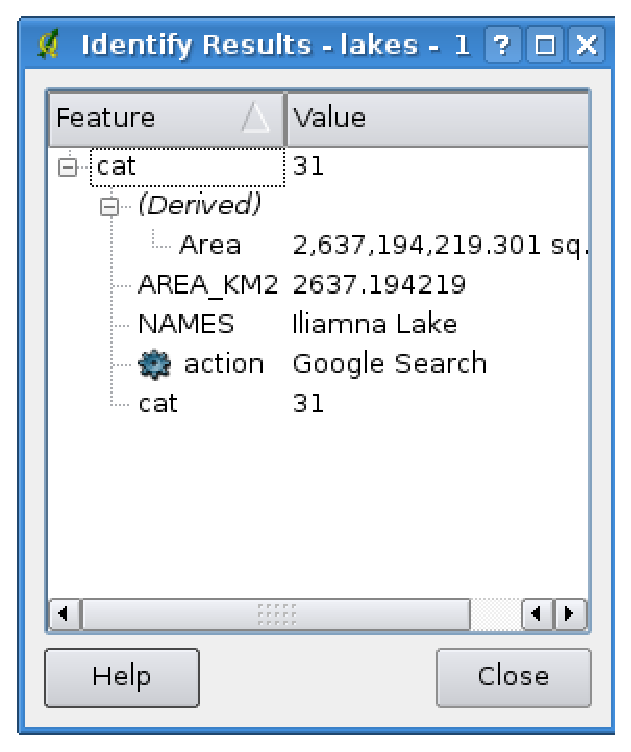
\includegraphics[clip=true, width=8cm]{action_identifyaction} 
\end{center}  
\end{figure}

Cuando hacemos clic en la acci\'on, se abre el Firefox y navega a la URL
\url{http://www.google.com/search?q=Tustumena}. Tambien es posible agregar mas 
campos de atributos a la acci\'on. Por lo tanto puede agregar un ``+'' al final del texto de la acci\'on, 
seleccione otro campo y haga clic en el bot\'on \button{Insert Field}. En este ejemplo no
hay otro campo disponible que tenga sentido que sea b\'uscado.

Puede definir m\'ultiples acciones para una capa y cada una se mostrar\'s en el
di\'alogo \dialog{Identify Results}. Puede tambien invocar acciones desde la tabla de atributos
seleccionando una l\'{\i}nea y haciendo clic, entonces eligiendo la acci\'on desde el men\'u
emergente.

Puede pensar en todos los tipos de usos para las acciones. Por ejemplo, si tiene una capa de puntos
que contenga lugares de im\'agenes o fotos junto con un nombre de archivo, puede
crear una acci\'on para lanzar el visualizador para mostrar la imagen. Tambien puede usar
acciones para lanzar reportes web para un campo de atributos o combinaci\'on de
campos, especificandolos en la misma forma que hicimos con el ejemplo de b\'usqueda en Google.

\subsubsection{Pesta\~na atributos}\index{attributes}\label{label_attributes}
Dentro de la pesta\~na \tab{Attributes} el conjunto de datos seleccionado puede ser manipulado.
Los botones \button{New Column} y \button{Delete Column} pueden ser usados,
cuando el conjunto de datos est\'a en modo de edici\'on. Al momento solo columnas
de capas Postgis pueden ser editados, debido a que esta funcionalidad no es soportada aun 
por la librer\'{\i}a the OGR. 

El bot\'on \button{Toggle editing mode} activa o desactiva este modo.

\minisec{edit widget}

Dentro de la pesta\~na \tab{Attributes} tambien encontrara un \texttt{edit widget} y una columna 
\texttt{value}. Estas dos columnas pueden ser usadas para definir valores o un rango 
de valores que son permitidos agregarse a las columnas de atributos de la tabla especifica. 
Son usadas para producir diferentes widgets de edici\'on en el di\'alogo de atributos. Estos 
widgets son:

\begin{itemize}
\item l\'{\i}nea de edici\'on: un campo de edici\'on que permite capturar texto simple (o restringir a 
n\'umero para atributos n\'umericos).
\item valor \'unico: una lista de atributos \'unicos de las caracter\'{\i}sticas existentes
es generada y presentada en una caja de selecci\'on para su selecci\'on.
\item  valor  \'unico (editable): una combinaci\'on de `l\'{\i}nea de edici\'on' y `valor \'unico'.
El campo de edici\'on completa los valores ingresados a un valor \'unico, pero tambien permite
escribir valores nuevos.
\item mapa de valores: una caja de selecci\'on para seleccionar desde un conjunto de valores especificados en la
columna \texttt{value} de la pesta\~na \tab{Attributes}.  Los posibles valores son 
delimitados por un punto y coma (ej. \verb|high;medium;low|). Tambien es posible
anteponer una etiqueta a cada valor, la cual es delimitada por signo de igual (ej.
\verb|high=1;medium=2;low=3|). La etiqueta se muestra en la caja de selecci\'on en lugar
del valor.
\item clasificaci\'on: si un renderer de valor \'unico es seleccionado para la capa, los valores
usados para las clases son presentados para selecci\'on en una caja de selecci\'on.
\item rango (editable): Un campo de edici\'on que permite restringir valores n\'umericos a un
rango dado.  El rango se especifica capturando un valor m\'{\i}nimo y un valor m\'aximo
delimitado por un punto y coma(ej. \verb|0;360|) en la columna \texttt{value} de
la pesta\~na \tab{Attributes}.
\item rango (slider): Se presenta un widget slider que permite la selecci\'on de un valor
en un rango y precisi\'on dado.  El rango es especificado por valores m\'{\i}nimo, m\'aximo
y un ancho de salto (ej. \verb|0;360;10|) en la columna \texttt{value} de
la pesta\~na \tab{Attributes}.
\item nombre de archivo: un widget de l\'{\i}nea de edici\'on acompa\~nado de un pulsador. Cuando est\'a
presionado permite seleccionar un nombre de archivo usando el di\'alogo de archivo estandar.
\end{itemize}

\subsubsection{Pesta\~na diagrama}\label{sec:diagram}
\index{vector layers!diagram}

La pesta\~na \tab{Diagram} te permite agregar un sobreposici\'on de gr\'aficos a una capa vectorial.
Para activar esta caracter\'{\i}stica, habra al Manejador de Complementos y selecciones el complemento  
de Sobreposici\'on de di\'agramas. Despues de esto, hay una nueva pesta\~na en el di\'alogo de vectores \dialog{Layer
Properties} donde las configuraciones para los diagramas pueden ser capturadas (vea 
la figura~\ref{fig:diagramtab}).

\begin{figure}[ht]
   \begin{center}
   \caption{El di\'alogo de propiedades de vector con la pesta\~na diagramas \nixcaption}\label{fig:diagramtab}\smallskip
   \includegraphics[clip=true, width=13cm]{diagram_tab}
\end{center}
\end{figure}

La implementaci\'on actual de di\'agramas provee soporte para barras, pastel
y para escalado lineal del tama\~no del diagrama de acuerdo a un atributo de
clasificaci\'on. Mostraremos un ejemplo la sobreposici\'on de un gr\'afico de barras
sobre la capa de l\'{\i}mites de Alaska.
Ambas capas vectoriales son parte del conjunto de datos de ejemplo de QGIS (vea
la Secci\'on~\ref{label_sampledata}.

\begin{enumerate}
\item Primero haga clic en el \'{\i}cono \toolbtntwo{mActionAddOgrLayer}{Load Vector},
navegue hasta el directorio con el conjunto de datos de ejemplo de QGIS y cargue las dos capas de vectores
\filename{alaska.shp} y \filename{climate.shp}.
\item Haga doble clic en la capa \filename{climate} en la leyenda del mapa y abra el di\'alogo
\dialog{Layer Properties}.
\item Haga clic en \tab{Diagram Overlay} y seleccione \button{Bar chart} como
tipo de diagrama.
\item En el diagrama necesitamos mostrar los valores de las tres columnas
\filename{T\_F\_JAN, T\_F\_JAN} y \filename{T\_F\_MEAN}. Primero seleccione
\filename{T\_F\_JAN} como atributos y haga clic \button{Add attribute}, entonces
\filename{T\_F\_JUL} y finalemente \filename{T\_F\_MEAN}.  
\item Para escalado lineal del tama\~no del diagrama definimos \filename{T\_F\_JUL}
como atributo de clasificaci\'on.
\item Ahora clic en \button{find maximum value}, elija el tama\~no y unidad y clic
\button{Apply} para mostrar el diagrama en la ventana principal de QGIS.
\item Ahora puede adaptar el tama\~no del gr\'afico, o cambiar los atributos de colores haciendo
doble clic en los valores de colores en el campo atributo.
Figure~\ref{fig:climatediagram} da una impresi\'on.
\item Finalmente haga clic \button{Ok}. 
\end{enumerate}

\begin{figure}[ht]
   \begin{center}
   \caption{Diagrama de datos de temperatura sobrepuesto en un mapa \nixcaption}\label{fig:climatediagram}\smallskip
   \includegraphics[clip=true, width=13cm]{climate_diagram}
\end{center}
\end{figure}

\subsection{Edici\'on}\index{editing}

QGIS suporta capacidades b\'asicas para la edici\'on de geometrias.  Antes de leer mas
deber\'{\i}a notar que en esta etapa el soporte para edici\'on es preliminar.
Antes de realizar cualquier edici\'on, realize siempre una copia de respaldo del conjunto de datos
a editar. 

\textbf{Note} - el procedimiento para editar capas de GRASS es diferente - vea la
Secci\'on \ref{grass_digitising} para detalles.

\subsubsection{Estableciendo la tolerancia del snapping y radio de b\'usqueda}

Antes de poder editar v\'ertices, es muy importante establecer la tolerancia
de snapping y radio de b\'usqueda a valores que permitan una \'optima edici\'on de
las geometr\'{\i}as de capas vectoriales. 

\minisec{Tolerancia de Snapping}

Tolerancia de Snapping es la distancia que QGIS usa para \usertext{search} el v\'ertice
mas cercano y/o segemento al cual tratas de conectar
cuando estableces un nuevo v\'ertice o mueve un v\'ertice existente. If you aren't
within the snap tolerance, QGIS will leave the vertex where you release the
mouse button, instead of snapping it to an existing vertex and/or segment. 

\begin{enumerate}
\item Una tolerancia de snapping general puede ser definida eligiendo
\mainmenuopt{Settings} > \dropmenuopttwo{mActionOptions}{Options}. 
(En Mac: vaya a  \mainmenuopt{QGIS} > Preferencias, en Linux: \mainmenuopt{Edit} > \dropmenuopttwo{mActionOptions}{Options}.)
En la pesta\~na de \tab{Digitizing} puede elegir entre v\'ertice a segmento o v\'ertice a
segmento y v\'ertice como mode de snap por defencto. Tambien puede definir una tolerancia de
snapping por defecto y un radio de b\'usqeuda para edici\'on de v\'ertices. La tolerancia puede ser establecida bien
en unidades de mapa o en pixeles.
En nuestro proyecto de digitalizaci\'on (trabajando con el conjunto de datos de Alaska),
las unidades estas en pies. Sus resultados pueden variar, pero algo en el
orden de 300 pies deber\'{\i}a estar bien a una escala de 1:10 000 y es una configuraci\'on razonable.
\item Una tolerancia de snapping basada en la capa puede ser definida eligiendo
\mainmenuopt{Settings} (or \mainmenuopt{File}) > \dropmenuopttwo{mActionOptions}{Project
Properties\dots}. En la pesta\~na \tab{General}, secci\'on \classname{Digitize} puede hacer clic
en \button{Snapping options\dots} para activar y ajustar el modo de snapping
y tolerancia en una capa (see Figure~\ref{fig:snappingoptions}).
\end{enumerate}

\begin{figure}[H]
   \begin{center}
   \caption{Editar opciones de snapping para una capa \nixcaption}\label{fig:snappingoptions}\smallskip
   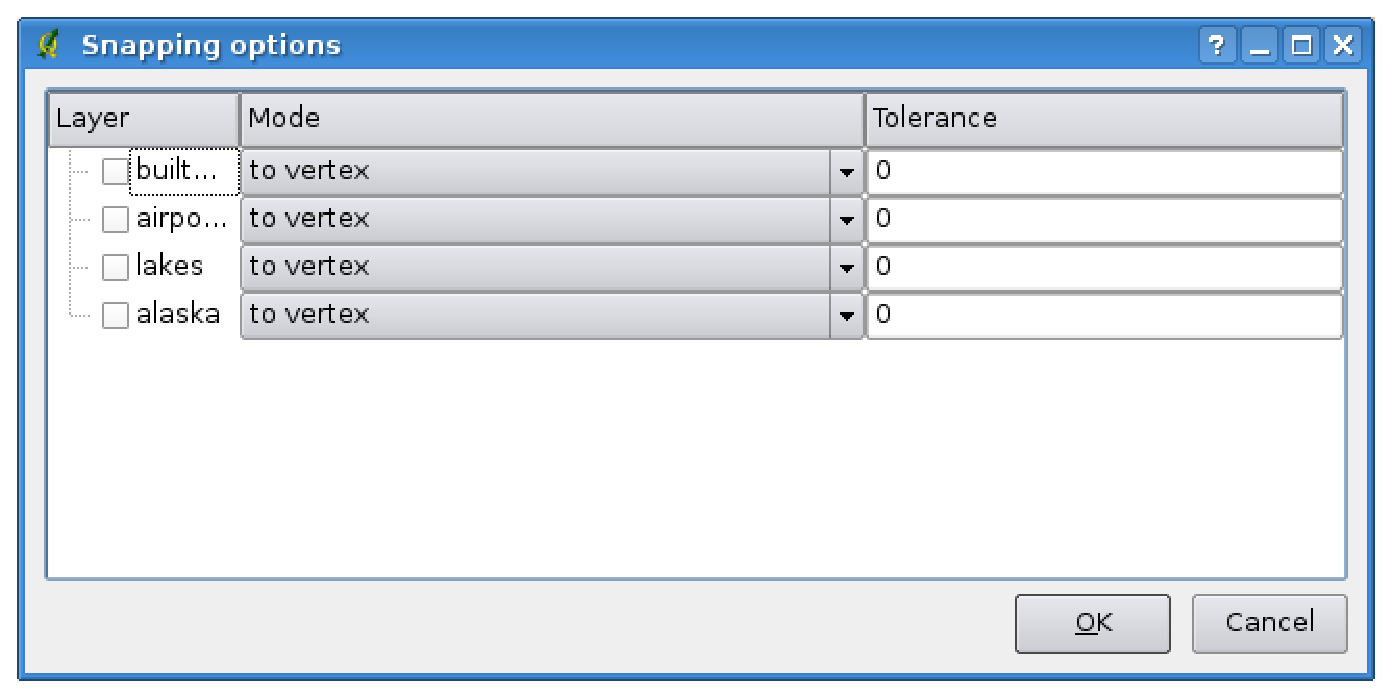
\includegraphics[clip=true, width=14cm]{editProjectSnapping} 
\end{center}  
\end{figure}

\minisec{Radio de b\'usqueda}

El radio de b\'usqueda es la distancia que QGIS usa para \usertext{search} el v\'ertice
mas cercano que se est\'a tratando de mover cuando se hace clic en el
mapa. Si no est\'a dentro del radio de b\'usqueda, QGIS no encontrar\'a y seleccionar\'a
ning\'un v\'ertice para edici\'on y mostrar\'a un molesto mensaje a tal efecto.
La tolerancia de snap tolerance y el radio de b\'usqueda pueden ser establecidos en unidades de mapa o pixeles, de esta manera puede
necesitar experimentar para establecerlos correctamente. Si especifica una tolerancia muy grande
QGIS puede snap al v\'ertice incorrecto, especialmente si est\'a tratando
con un gran n\'umero de v\'ertices muy proximos. Establecer un radio de b\'usqueda muy
peque\~no no encontrar\'a nada a mover.

El radio de b\'usqueda para ediciones de vertices en unidades de capa puede ser definido en la
pesta\~na \tab{Digitizing} bajo \mainmenuopt{Settings} >
\dropmenuopttwo{mActionOptions}{Options}. El mismo lugar donde defini\'o la
tolerancia de snapping general para el proyecto.

\subsubsection{Edici\'on topol\'ogica}

Ademas de las opciones basadas en capa la pesta\~na \tab{General} en el men\'u 
\mainmenuopt{Settings} -> \dropmenuopttwo{mActionOptions}{Project Properties\dots} 
tambien provee algunas funcionalidades topol\'ogicas. 
En el grupo de opciones Digitalizaci\'on puede \checkbox{Activar edici\'on topol\'ogica} y/o activar 
\checkbox{Evitar intersecciones de nuevos pol\'{i}gonos}.

\minisec{Activar edici\'on topol\'ogica}

La opci\'on \checkbox{Activar edici\'on topol\'ogica} es para editar y mantener 
l\'{\i}mites comunes en mosaicos de pol\'{\i}gonos. QGIS "detecta" un l\'{\i}mite compartido en 
un mosaico de pol\'{\i}gonos y solo tiene que mover el v\'ertice una sola vez y QGIS se encargar\'a 
de actualizar el otro l\'{\i}mite.

\minisec{Evitar intersecciones de nuevos pol\'{\i}gonos}

La segunda opci\'on topol\'ogica llamada \checkbox{Evitar intersecci\'on de nuevos pol\'{\i}gonos} 
evita traslapes en mosaicos de pol\'{\i}gonos. Es para digitalizaci\'on r\'apida de pol\'{\i}gonos adyacentes. 
Si ya tiene un pol\'{\i}gono, es posible con esta opci\'on digitalizar la segunda 
de tal forma que las dos se intersecten y Qgis entonces corta el segundo pol\'{i}gono en el l\'{i}mite com\'un. 
La ventaja es que los usuarios no tienen que digitalizar todos los v\'ertices del l\'{i}mite com\'un.

\subsubsection{Edici\'on de una capa existente}
\index{vector layers!editing}
\index{editing!an existing layer}
\label{sec:edit_existing_layer}

Por defecto, QGIS carga capas como solo lectura: Esto es una medida de seguridad
para evitar editar accidentalmente una capa si hay un dezlis del mouse.
Sin embargo, puede elegir editar una capa siempre y cuando el proveedor de datos lo soporte,
y el conjunto de datos sea escribible (ej. sus archivos no son de solo escritura).

La edici\'on de capas es mas versatil cuando es usada en conjuntos de datos PostgreSQL/PostGIS. 

\begin{Tip}[ht]\caption{\textsc{Integridad de datos}}
\qgistip{Siempre es una buena idea respaldar su conjunto de datos antes de iniciar 
la edici\'on. Mientras los autores de QGIS han realizado cada esfuerzo para preservar 
la integridad de sus datos, no se ofrece garant\'{\i}a en este aspecto.
}
\end{Tip}

\begin{Tip}[ht]\caption{\textsc{Manipulando datos de atributos}}
\qgistip{Actualmente solo capas de PostGIS son soportadas para agregar y eliminar columnas de atributos
dentro de este di\'alogo. En versiones futuras de QGIS, otros conjuntos de datos ser\'an soportados, 
porque esta funcionalidad fue recientemente implementada en GDAL/OGR > 1.6.0
}
\end{Tip}



\begin{Tip}[ht]\caption{\textsc{Guarde regularmente}}
\qgistip{Recuerde desactivar \toolbtntwo{mActionToggleEditing}{Toggle editing} regularmente.  
Esto le permite guardar los cambios recientes,
y tambien confirmar que los conjuntos de datos pueden aceptar todos los cambios.
}
\end{Tip}

\begin{Tip}[ht]\caption{\textsc{Ediciones concurrentes}}
\qgistip{Esta versi\'on de QGIS no rastrea si alguien mas est\'a editando una caracter\'{i}stica al mismo tiempo
que usted.  La \'ultima persona en guardar su edici\'on gana.
}
\end{Tip}

\begin{Tip}[ht]\caption{\textsc{Haga un acercamiento antes de empezar a editar}}
\qgistip{Antes de editar una capa, deber\'{\i}a hacer un acercamiento
a su \'area de inter\'es. Esto evita esperar mientras los marcadores de v\'ertices 
son dibujados en la capa completa.
}
\end{Tip}

\begin{Tip}[ht]\caption{\textsc{Marcadores de v\'ertices}}
\qgistip{
La versi\'on actual de QGIS soporta dos tipos de marcadores de v\'ertices 
un c\'irculo semi-transparente o una cruz. Para cambiar el estilo de marcador, elija
\dropmenuopttwo{mActionOptions}{Options} del men\'u
\mainmenuopt{Settings} y haga clic en la pesta\~na \tab{Digitizing} y selecciones
la entrada apropiada.
}
\end{Tip}

Todas las sesiones de edici\'on comienzan eligiendo la opci\'on \dropmenuopttwo{mActionToggleEditing}{Toggle editing}.
Esta puede ser encontrada en el men\'u contextual haciendo clic derecho en la entrada para esa capa en la leyenda.
\index{Allow Editing}
Alternativamente, puede usar el bot\'on \index{Toggle Editing}
\toolbtntwo{mActionToggleEditing}{Toggle editing} de la barra de herramientas para empezar o parar 
el modo de edici\'on.\index{editing!icons} Una vez que la capa est\'a en modo de edic\'on, 
los marcadores aparecer\'an en los v\'ertices, y botones adicionales en la barra de herramientas 
estar\'an disponibles.

\minisec{Haciendo zoom y pan con la rueda del rat\'on}

Mientras esta digitalizando puede presionar la rueda del rat\'on para hacer un pan dentro de la ventana
principal y puede girar la rueda para acercarse o alejarse en el mapa. Para alejarse
posicione el cursor del rat\'on dentro del \'area del mapa y gire hacia atras (hacia usted) 
para acercarse gire la rueda del rat\'on hacia afuera (alejandose de usted). La posici\'on del cursor del mouse ser\'a el centro 
del zoom al \'area de inter\'es. Puede personalizar el comportamiento 
de la rueda del mouse usando la pesta\~na \tab{Map tools} bajo el men\'u
\mainmenuopt{Settings} >\dropmenuopt{Options}.  

\minisec{Desplazamiento con las teclas de flechas}

Es posible desplazar el mapa  durante la digitalizaci\'on con las teclas de flecha. Posicione
el cursor del mouse dentro del \'area de mapa presione la flecha derecha para hacer un
desplazamiento al este, tecla de flecha izquierda para desplazarse al oeste, tecla de flecha hacia arriba para desplazarse al norte y flecha hacia abajo 
para desplazarse al sur.

Tambien puede usar la barra espaciadora para temporalmente causar movimientos del mouse para hacer desplazamientos 
al mapa. Las teclas PgUp y PgDown en su teclado causar\'an que la vista se acerque 
o aleje sin interrumpir su sesi\'on de digitalizaci\'on.

You can perform the following editing functions:

\begin{itemize}
\item Add Features: \toolbtntwo{mActionCapturePoint}{Capturar Punto},
  \toolbtntwo{mActionCaptureLine}{Capturar L\'{\i}nea} y
  \toolbtntwo{mActionCapturePolygon}{Capturar Pol\'{\i}gono}
\item \toolbtntwo{mActionAddRing}{Agregar Anillo}
\item \toolbtntwo{mActionAddIsland}{Agregar Isla}
\item \toolbtntwo{mActionSplitFeatures}{Partir Caracter\'{\i}sticas}
\item \toolbtntwo{mActionMoveFeature}{Mover Caracter\'{\i}sticas}
\item \toolbtntwo{mActionMoveVertex}{Mover V\'ertice}
\item \toolbtntwo{mActionAddVertex}{Agregar V\'ertice}
\item \toolbtntwo{mActionDeleteVertex}{Eliminar V\'ertice}
\item \toolbtntwo{mActionDeleteSelected}{Eliminar Seleccionado}
\item \toolbtntwo{mActionEditCut}{Cortar Caracter\'{\i}sticas}
\item \toolbtntwo{mActionEditCopy}{Copiar Caracter\'{\i}sticas}
\item \toolbtntwo{mActionEditPaste}{Pegar Caracter\'{\i}sticas}
\end{itemize}

\minisec{Agregando Caracter\'{\i}sticas}
\index{vector layers!adding!feature}

Antes de iniciar agregando caracter\'{\i}sticas, use las herramientas \toolbtntwo{mActionPan}{pan}
y \toolbtntwo{mActionZoomIn}{zoom-in}/\toolbtntwo{mActionZoomOut}{zoom-out} 
para navegar al \'area de inter\'es.

Entonces puede usar los \'{\i}conos \toolbtntwo{mActionCapturePoint}{Capturar punto},
\toolbtntwo{mActionCaptureLine}{Capture l\'{\i}nea} o
\toolbtntwo{mActionCapturePolygon}{Capturar pol\'{\i}gono} en la barra de herramientas para poner el cursor de QGIS
en modo de digitalizaci\'on.

Para cada caracter\'{\i}sticas, primero digitaliza la geometr\'{\i}a, despues captura sus atributos.

Para digitalizar la geometr\'{\i}a, haga clic izquierdo en el \'area del mapa para crear el primer
punto de su nueva caracter\'{\i}stica.

Para l\'{\i}neas y pol\'{\i}gonos, siga haciendo clic izquierdo para cada punto adicional
que desee capturar. Cuando haya finalizado de agregar puntos,
haga clic derecho en cualquier parte del \'area de mapa para confirmar que ha terminados de meter
la geometr\'{i}a de esa caracter\'{\i}stica.

La ventana de atributos aparecer\'a, permitiendole meter la informaci\'on de la nueva caracter\'{\i}stica.
Figure \ref{fig:vector_digitising} muestra como establecer atributos para un nuevo rio ficticio
en Alaska.

\begin{figure}[ht]
   \begin{center}
   \caption{Di\'alogo de Captura de Atributos despues de digitalizar una nueva caracter\'{\i}stica vectorial
   \nixcaption}\label{fig:vector_digitising}\smallskip
   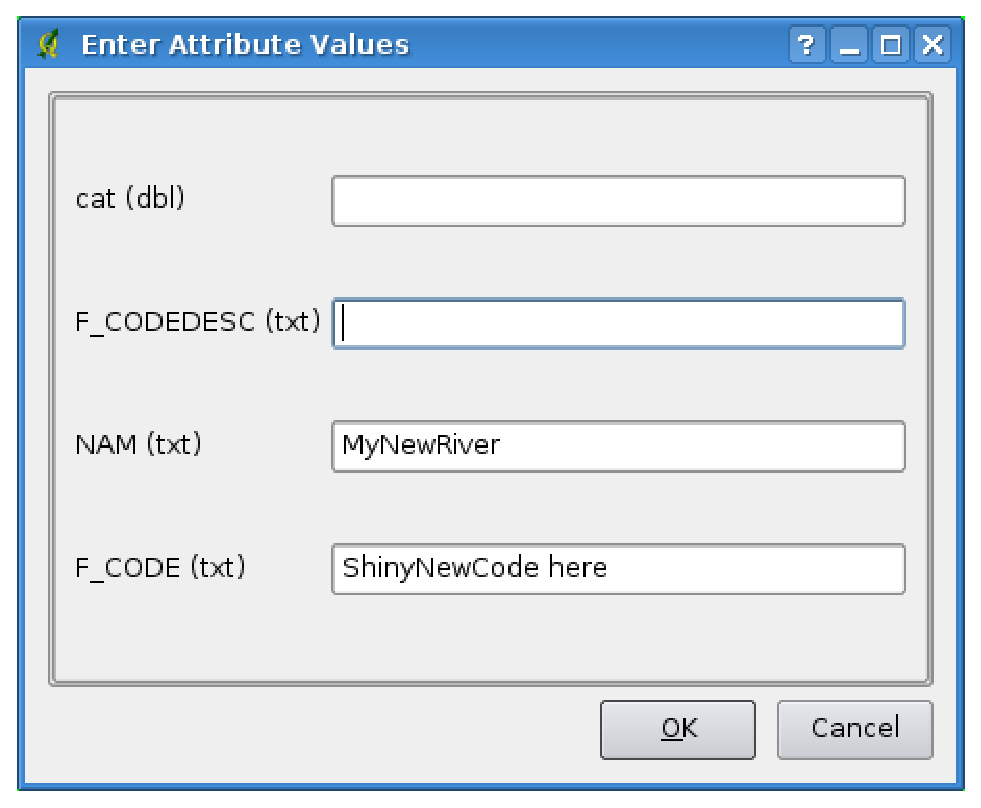
\includegraphics[clip=true, width=8cm]{editDigitizing}
\end{center}  
\end{figure}

\begin{Tip}[ht]\caption{\textsc{Tipos de Valores de Atributos}}
\qgistip{
Al menos para edici\'on de shapefiles los tipos de atributos son validados durante la
captura. Por esto, no es posible capturar un n\'umero dentro de una columna de texto en el di\'alogo
\dialog{Capturar Valores de Atributos} o viceversa. Si necesita hacerlo as\'{\i},
deber\'{\i}a editar los atributos en un segundo paso dentro del di\'alogo \dialog{Attribute
table}.
}
\end{Tip}

\minisec{Mover Caracter\'{\i}stica}
\index{vector layers!move!feature}

Puede mover caracter\'{\i}sticas usando el \'{\i}cono \toolbtntwo{mActionMoveFeature}{Move Feature} 
de la barra de herramientas.

\minisec{Partir Caracter\'{\i}stica}
\index{vector layers!split!feature}

Puede partir caracter\'{\i}sticas usando el \'{\i}cono \toolbtntwo{mActionSplitFeatures}{Split Features}
de la barra de herramientas.

\minisec{Editando V\'ertices de una Caracter\'{\i}stica}
\index{vector layers!editing!vertex}

Para ambos tipos de capas PostgreSQL/PostGIS y  shapefile, los v\'ertices de las caracter\'{\i}sticas pueden ser editados. 

Los v\'ertices pueden ser directamente editados, esto es, no tiene
que elegir cual nueva caracter\'{\i}stica editar antes de que pueda cambiar
su geometr\'{\i}a.
En algunos casos, m\'ultiples caracter\'{\i}sticas pueden compartir el mismo v\'ertice
y de esta manera los siguientes reglas aplican cuando el mouse es presionado
cerca de caracter\'{\i}sticas del mapa:

\begin{itemize}
\item \textbf{L\'{\i}neas}    - La l{\'i}nea mas cercana a la posici\'on del rat\'on
                          es usada como caracter\'{\i}stica objetivo.
                          Entonces (para mover y eliminar un v\'ertice)
                          el v\'ertice mas cercano
                          en esa l\'{\i}nea es el objetivo de edici\'on.

\item \textbf{Pol\'{\i}gonos} - Si el rat\'on est\'a dentro del pol\'{\i}gono, entonces este
                          es la caracter\'{\i}stica objetivo; de lo contrario el pol\'{\i}gono mas cercano
                          es usado.
                          Entonces (para mover y eliminar un v\'ertice)
                          el v\'ertice mas cercano
                          en ese pol\'{\i}gono es el objetivo de edici\'on.                          
\end{itemize}

Necesitar\'a establecer la propiedad
\mainmenuopt{Settings}>\dropmenuopttwo{mActionOptions}{Options}>\tab{Digitalizando}>\selectnumber{Radio de b\'usqueda}{10}
a un n\'umero mayor que cero.  De lo contrario QGIS no podr\'a decir que caracter\'{\i}stica esta siendo editeda.


\minisec{Agregando V\'ertices de una Caracter\'{\i}stica}
\index{vector layers!adding!vertex}

Puede agregar nuevos v\'ertices a una caracter\'{\i}stica usando el \'{\i}cono
\toolbtntwo{mActionAddVertex}{Add Vertex} 
de la barra de herramientas.

Note que, no tiene sentido agregar mas v\'ertices a una caracter\'{\i}stica de punto!

En esta versi\'on de QGIS, los v\'ertices solo pueden ser agregados a un \textit{existing} segmento
de una caracter\'{\i}stica de l\'{\i}nea.  Si quieres extender una l\'{\i}nea mas all\'a de su final,
necesitaras primero mover el v\'ertice final, entonces agrega un nuevo v\'ertice donde
el terminal solia estar.

\minisec{Moviendo V\'ertices de una Caracter\'{\i}stica}
\index{vector layers!moving!vertex}

Puede mover v\'ertices usando el \'{\i}cono \toolbtntwo{mActionMoveVertex}{Mover V\'ertice}
de la barra de herramientas.

\minisec{Eliminando V\'ertices de una Caracter\'{\i}stica}
\index{vector layers!deleting!vertex}

Puede eliminar v\'ertices usando el \'{\i}cono \toolbtntwo{mActionDeleteVertex}{Delete Vertex}
de la barra de herramientas.

Note que, no tiene sentido eliminar el v\'ertice de una caracter\'{\i}stica de Punto!
En lugar de eso elimine la caracter\'{\i}stica completa.

Similarment, una l\'{\i}nea de un solo v\'ertice o pol\'{\i}gono de dos v\'ertices tambien es
bastante inutil y llevar\'a a resultados impredecibles en alg\'un otro lugar
QGIS, as\'{\i} que no lo haga.

\textbf{advertencia:} Un v\'ertice es identificado para eliminaci\'on tan pronto 
como haces clic con el rat\'on cerca de una caracter\'{\i}stica elegible.
Para deshacer, necesitaras desactivar
la edici\'on y despues descartar sus cambios.
(Claro esto significar\'a que otros cambios sin guardar ser\'an perdidos, tambien.)

\minisec{Agregar Anillo}
\index{vector layers!add!ring}

Puede crear pol\'{\i}gonos anillo usando el \'{\i}cono \toolbtntwo{mActionAddRing}{Add Ring}
de la barra de herramientas. Esto significa que dentro de un \'area existente es posible digitalizar
otros pol\'{\i}gonos, esto ocurrir\'a como un 'todo', de esta manera solo 
el \'area entre los l\'{\i}mites del pol\'{\i}gono mas externo y el mas interno permanecen 
como un pol\'{\i}gono de anillo. 

\minisec{Agregar Isla}
\index{vector layers!add!island}

Puede \toolbtntwo{mActionAddIsland}{agregar isla} a seleccionados multipol\'{\i}gonos. 
El nuevo pol\'{\i}gono isla tiene que ser digitalizado fuera del multipol\'{\i}gono seleccionado. 

\minisec{Cortando, Copiando y Pegando Caracter\'{\i}sticas}
\index{vector layers!cut!feature}
\index{vector layers!copy!feature}
\index{vector layers!paste!feature}
\index{editing!cutting features}
\index{editing!copying features}
\index{editing!pasting features}

Las caracter\'{\i}sticas seleccionadas pueden ser cortadas, copiadas y pegadas entre capas en el mismo proyecto
de QGIS, siempre y cuado de antemano las capas de destino han sido establecidas a 
\toolbtntwo{mActionToggleEditing}{Activar edici\'on}.

Las caracter\'{\i}stica pueden tambien ser pegadas a aplicaciones externas como texto:  Esto es,
las caracter\'{\i}sticas son presentadas en formato CSV con los datos de geometr\'{\i}a 
en el formtado Well-Known Text (WKT) de la OGC.


Sin embargo en esta version de QGIS, texto de caracter\'{\i}sticas de fuera de QGIS no pueden 
ser pegadas a una capa dentro de QGIS. ?`Cuando seria \'util la funci\'on de copiar y pegar? 
Bien, resulta que puede editar mas de una capa 
al tiempo que copia y pega caracter\'{\i}sticas entre capas. ?`Por qu\'e querriamos hacer
eso?  dicho que tenemos que hacer una trabajo sobre una nueva capa pero solo necesita uno o
dos lagos, no los 5,000 en nuestra capa \filename{big\_lakes}. Podemos crear una nueva capa
y usar copiar/pegar para soltar los lagos necesarios en ella. 

Como un ejemplo estamos copiando algunos lagos a una nueva capa:

\begin{enumerate}
\item Cargue la capa de la que desea copiar (capa fuente)
\item Cargue o cree la capa a la que desea copiar (capa destino) 
\item Inicie la edici\'on para la capa destino
\item Haga la capa fuente activa haciendo clic en ella en la leyenda 
\item Use la herramienta \toolbtntwo{mActionSelect}{Seleccionar} para seleccionar la caracter\'{\i}sticas(s) en la capa fuente
\item Haga clic en la herramienta \toolbtntwo{mActionEditCopy}{Copy Features}
\item Haga la capa destibo activa haciendo clic en ella en la leyenda 
\item Haga clic en la herramienta \toolbtntwo{mActionEditPaste}{Paste Features}
\item Pare la edici\'on y guarde los cambios
\end{enumerate}

?`Qu\'e pasa si las capas fuentes y destino tienen
diferentes esquemas (no son iguales los nombres de campos y tipos)? QGIS llena
lo que coincide e ignora el resto. Si no le interesa los atributos
siendo copiados a la capa destino, no importa como dise\~ne los
campos y los tipos de datos. Si desea asegurarse que todo - caracter\'{\i}sticas y sus
atributos - son copiados, aseg\'urese que los esquemas coincidan.

\begin{Tip}[ht]\caption{\textsc{Congruencia de Caracter\'{\i}sticas Pegadas}}
\qgistip{Si sus capas de fuente y destino usan la 
misma proyecc\'on, entonces las caracter\'{\i}sticas pegadas tendr\'an
una geometr\'{\i}a id\'entica a la capa fuente.
Sin embargo si la capa destino tiene una proyecci\'on diferente
entonces QGIS no puede garantizar que la geometr\'{\i}a es identica.
Esto es simplemente porque hay peque\~nos errores de redondeo
envolucrados durante la conversi\'on entre proyecciones.
}
\end{Tip}

\minisec{Eliminado Caracter\'{\i}sticas Seleccionadas}
\index{vector layers!deleting!feature}

Si deseamos eliminar un pol\'{\i}gono completo, podemos hacerlo primero seleccionando 
el pol\'{\i}gono usando la herramienta regurla \toolbtntwo{mActionSelect}{Select Features}. Puede seleccionar 
m\'ultiples caracter\'{\i}sticas para su eliminaci\'on. Una vez que ha establecido la selecci\'on, use la 
herramienta \toolbtntwo{mActionDeleteSelected}{Eliminar Seleccionado} para eliminar las caracter\'{\i}sticas. No hay funci\'on deshacer, 
pero recuerde que su capa no ha cambiado realmente hasta que pare la edici\'on y elija 
guardar los cambios. De esta manera si comete alg\'un error, siempre puede cancelar el guardado.

La herramienta \toolbtntwo{mActionEditCut}{Cortar Caracter\'{\i}sticas} en la barra de herramientas de digitalizaci\'on puede
tambien ser usada para eliminar caracter\'{\i}sticas. Esto efectivamente elimina la caracter\'{\i}sticas pero
tambien la coloca en un lugar especial llamado ``portapapeles espacial". De esta manera cortamos la caracter\'{\i}stica a eliminar. 
Podemos entonces usar la \toolbtntwo{mActionEditPaste}{herramienta pegar} para regresarla, d\'andonos un deshacer de un nivel 
capability. Cut, copy, and paste work on the currently selected features, 
significando que podemos operar en mas de una al mismo tiempo.

\begin{Tip}[ht]\caption{\textsc{Soporte para la Eliminaci\'on de Caracter\'{\i}sticas}}
\qgistip{Cuando se edita ESRI shapefiles, el borrado
de caracter\'{\i}sticas solo trabaja si QGIS est\'a compilado con una versi\'on de GDAL version 1.3.2 o mayor. 
Las versiones de OS X y Windows QGIS disponibles en el sitio de descarga estan compilados 
usando GDAL 1.3.2 o mayor.
}
\end{Tip}

\minisec{Modo Snap}
\index{editing!snap}
QGIS permite que los v\'ertices digitalizados sean snapped a otros v\'ertices de la misma capa. Para 
establecer la tolerancia de snapping, vaya a
\mainmenuopt{Settings}>\dropmenuopttwo{mActionOptions}{Options}->\tab{Digitizing}.
(En Mac: vaya a  \mainmenuopt{QGIS} > Preferencias, En Linux: \mainmenuopt{Edit} > \dropmenuopttwo{mActionOptions}{Options}.)
Note que la tolerancia de snapping est\'a en unidades de mapa o pixeles.

\minisec{Guardadno Capas Editadas}
\index{editing!saving changes}

Cuando una capa est\'a en modo de edici\'on, cualquier cambio permanece pendiente en la memoria de QGIS.
Por lo tanto no se guardan o se les aplica un commit inmediatamente al conjunto de datos o disco.
Cuando desactiva la edici\'on (o sale de QGIS para el caso), 
se le pregunta si desea guardar sus cambios o
descartarlos.

Si los cambios no pueden ser guardados (ej. disco lleno, o los atributos tienen
valores fuera de rango), el estado de memoria de QGIS es preservado.  Esto
permites que ajuste su edici\'on y lo intente de nuevo.

\subsubsection{Creando una nueva capa}\label{sec:create shape}\index{editing!creating a new layer}

Para crear una nueva capa para edici\'on, elija \toolbtntwo{mActionNewVectorLayer}{New Vector Layer} del
\mainmenuopt{Layer} men\'u. 
Se mostrar\'a un dia\'alogo \dialog{New Vector Layer} como el de la
Figura \ref{fig:newvectorlayer}. Elija el tipo de capa (point,
line o polygon).

\begin{figure}[ht]
   \begin{center}
   \caption{Di\'alogo creando una nueva capa \nixcaption}\label{fig:newvectorlayer}\smallskip
   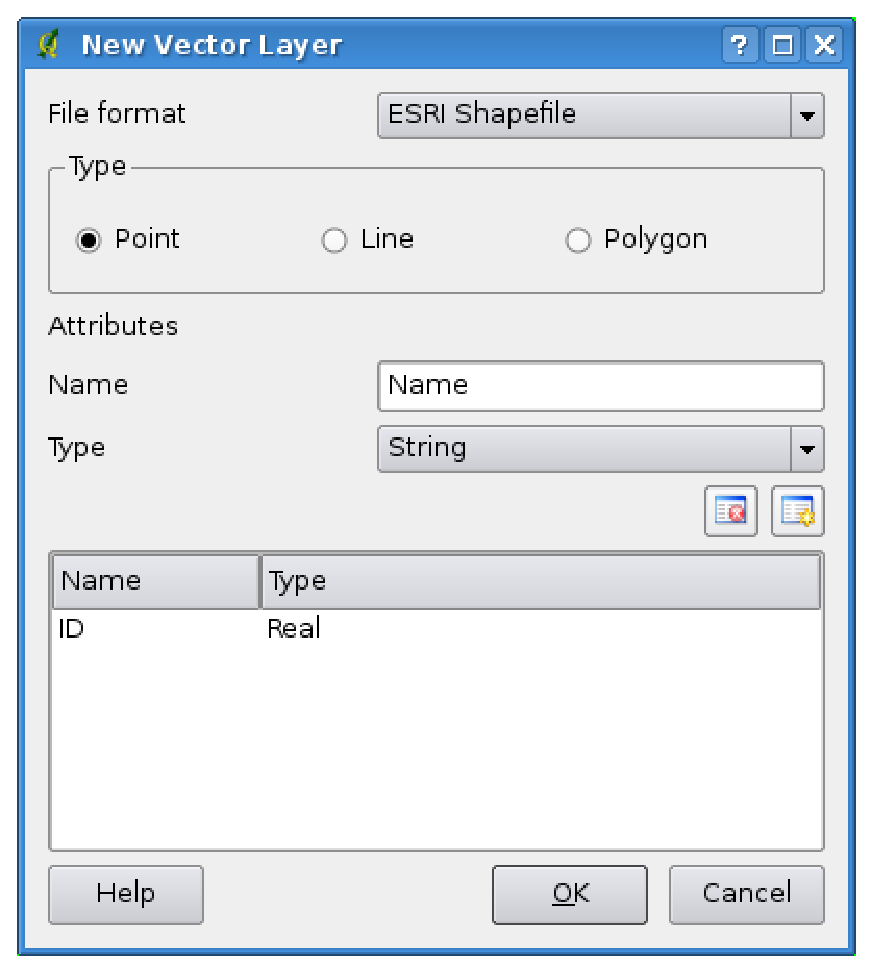
\includegraphics[clip=true, width=10cm]{editNewVector}
\end{center} 
\end{figure}

Note que QGIS no soporta aun la creaci\'on de
caracter\'{\i}sticas 2.5D (ej. caracter\'{\i}sticas con coordenadas X,Y,Z) o caracter\'{\i}sticas de medidas.
A la fecha solo pueden ser creados shapefiles. En una futura versi\'on de QGIS, la creaci\'on de cualquier tipo
de capa OGR o PostgreSQL ser\'a soportado. 

La creaci\'on de capas GRASS es soportada dentro del complemento de GRASS. Vea la secci\'on 
\ref{sec:creating_new_grass_vectors} para mas informaci\'on de creaci\'on de capas GRASS.

Para completar la creaci\'on de una nueva capa, agregue los atributos deseados haciendo
clic en el bot\'on  \button{Add} y especificando un campo y el tipo para al atributo.
Solo los tipos de atributos \selectstring{Type}{real}, \selectstring{Type}{integer}, y \selectstring{Type}{string} son soportados. Una vez que esta contento con sus atributos,
haga clic en \button{OK} y provea un nombre para el shapefile.
QGIS autom\'aticamente agregar\'a una extensi\'on \filename{.shp} al nombre que especific\'o. Una vez
que la capa ha sido creada, ser\'a agregada al mapa y puede ser editada en la misma forma
que se describe en la Secci\'on anterior \ref{sec:edit_existing_layer}. 

\subsubsection{Trabajando con la tabla de atributos}\label{sec:attribute table}\index{editing!working with the attribute table}

Para abrir la tabla de atributos para una capa vectorial, haga la capa activa haciendo clic en ella en el \'area de leyenda del mapa. 
Entonces use el men\'u  capa\mainmenuopt{Layer} del men\'u principal y elija \dropmenuopttwo{mActionOpenTable}{Open Attribute Table} 
desde el men\'u. Tambien es posible hacer clic derechi en la capa y elegir \dropmenuopttwo{mActionOpenTable}{Open Attribute Table} 
desde el men\'u desplegable. Esto abrir\'a una nueva ventana que mostrar\'a los atributos para cada caracter\'{\i}stica en la capa 
(figure \ref{fig:attributetable}).

\begin{figure}[ht]
   \begin{center}
   \caption{Tabla de atributos para la tabla de Alaska \nixcaption}\label{fig:attributetable}\smallskip
   \includegraphics[clip=true, width=12cm]{vectorAttributeTable}
\end{center} 
\end{figure}

Cada columna puede ser ordenada haciendo clic en su encabezado. Una peque\~na flecha indica el orden 
(apuntando hacia abajo significa valores descendentes de la primara columna hacia abajo, apuntando hacia arriba significa valores ascendentes desde la primera columna hacia abajo). 
Para una selecci\'on simple de atributos en una columna el bot\'on \button{Look for} 
puede ser usado. Seleccione el campo (columna) en la cual la b\'usqueda ser\'a realizada 
el men\'u desplegable y presione el bot\'on \button{Search}. Para b\'usquedas mas complejas use
el bot\'on B\'usquedas Avanzadas \button{...}, el cual lanzar\'a el Constructor de Consultas de B\'usqueda descrito en 
la Secci\'on \ref{sec:select_by_query}. 

Para solo mostrar los registros, use la caja de selecci\'on \checkbox{Show selected records only}.
Usando los botones en la parte izquierda inferior de la ventana, seleccione los campos que ser\'an removidos, 
movidos a la parte superior de la tabla, o la selecci\'on que ser\'a invertida. Las caracter\'{\i}sticas seleccionadas pueden ser movidas, copiadas al portapapeles, tambien puede ser hecho con \keystroke{Ctrl-C}. Puede hacer zoom 
a las caracter\'{\i}sticas seleccionadas en el mapa. Activando la edici\'on permite editar valores de atributos. 

\subsection{Constructor de consultas}\label{sec:query_builder}
\index{Query Builder}

El Constructor de Consultas permite definir un conjunto de una tabla y mostrarlo como una capa en QGIS. Actualmente solo puede ser usado con capas PostGIS. 
Por ejemplo, si se tiene una capa \filename{towns} con un campo \usertext{population} se puede seleccionar solo ciudades grandes escribiendo \usertext{population > 100000} en la caja SQL del constructor de consultas. Figura
\ref{fig:query_builder} muestra un ejemplo del constructor de consultas llenado con datos de una capa PostGIS con atributos almacenada en PostgreSQL. 

\begin{figure}[ht]
  \begin{center}
    \caption{Query Builder \nixcaption}\label{fig:query_builder}\smallskip
    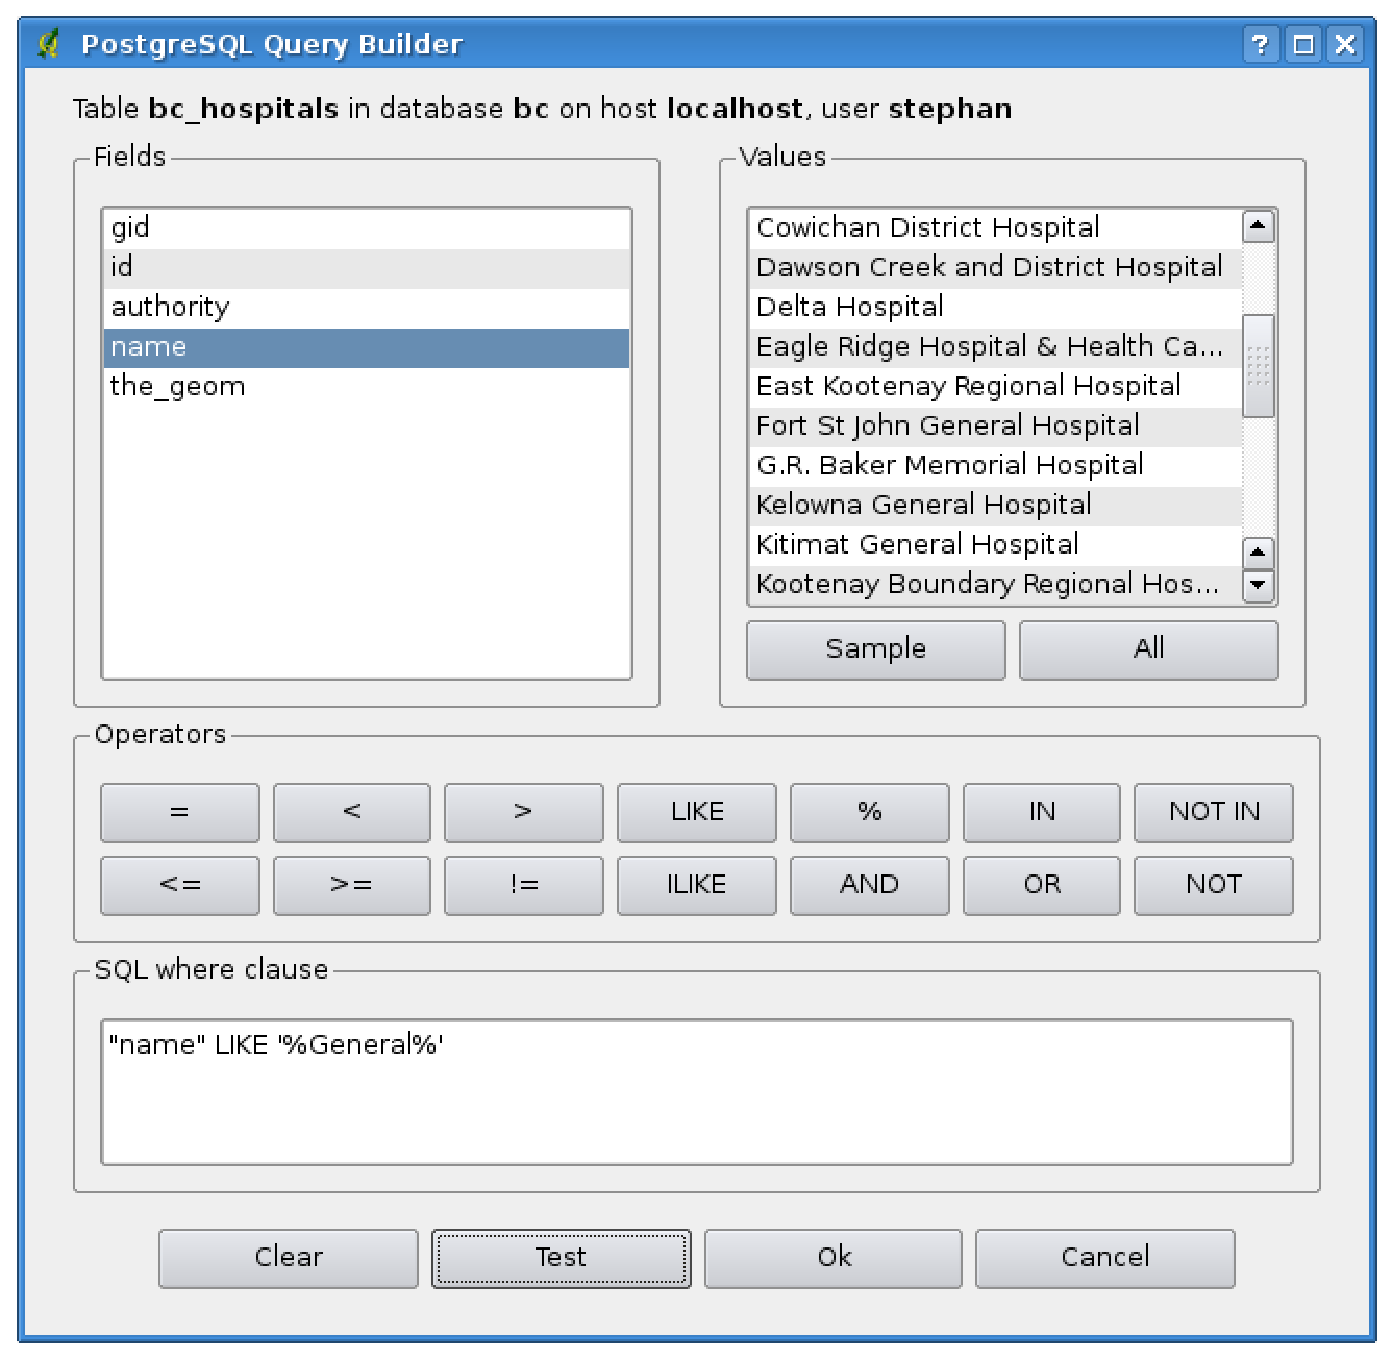
\includegraphics[clip=true, width=11.5cm]{queryBuilder}
  \end{center}  
\end{figure}

El constructor de consultas \index{Query Builder} muestra los campos de la capa de la base de datos en una lista en la izquierda. Puede obtener un ejemplo de los datos contenidos en el campo resaltado haciendo clic en el bot\'on \button{Sample} \index{Query
Builder!generating sample list}. Esto recupera los primeros 25 valores distintos para el campo desde la base de datos. Para obtener una lista de todos los posibles valores para un campo, haga clic en el bot\'onf \button{All} \index{Query Builder!getting all
values}. Para agregar un campo seleccionado o valor a la consulta, haga doble clic en el\index{Query Builder!adding fields}. Puede usar varios botones para construir la consulta o puede escribirla dentro de la caja SQL.

Para probar una consulta, haga clic en el bot\'on \button{Test} \index{Query Builder!testing
queries}. Esto regresar\'a un conteo del n\'umero de registros que pueden ser incluidos en la capa. Cuando est\'e satisfecho con la consulta, haga click en el bot\'on \button{OK}. El SQL para la clausula where ser\'a mostrada en la columna SQL de la lista de capas.

\begin{Tip}\caption{\textsc{Changing the Layer Definition}}\index{Query
Builder!changing layer definitions}
\qgistip{You can change the layer definition after it is loaded by altering
the SQL query used to define the layer. To do this, open the 
vector \dialog{Layer Properties} dialog by double-clicking on the layer in the legend and click on the
\button{Query Builder} button on the \tab{General} tab. See Section
\ref{sec:vectorprops} for more information.}
\end{Tip}

\subsection{Selecci\'on por consulta}\label{sec:select_by_query}
\index{PostgreSQL!query builder}
\index{PostGIS!query builder}
\index{query builder!PostgreSQL}
\index{query builder!PostGIS}

Con QGIS es tambien posible seleccionar caracter\'isticas usando una interface similar al constructor de consultas utilizado en \ref{sec:query_builder}. En la secci\'on superior el proposito el prop\'osito del constructor de consultas es solo mostrar las caracter\'{\i}sticas cumpliendo el filtro de ser un subconjunto de una 'capa virtual'. El prop\'osito de la funci\'on de consulta seleccionar por es la de resaltar todas las caracter\'{\i}sticas que cumplan con un criterio particular. Seleccionar por consulta puede ser usado con todos los complementos proveedores de datos.

Para hacer una 'selecci\'on por consulta' en una capa cargada, haga clic en el bot\'on \toolbtntwo{mActionOpenTable}{Open Table} para abrir la tabla de atributos de la capa. Entonces clic en el bot\'on \button{Advanced...} en la parte inferior. Esto inicia el Constructor de Consultas que permite definir un subconjunto de una tabla y mostrarlo como se describe en la Secci\'on \ref{sec:query_builder}.


\index{vector layers|)}

% vim: set textwidth=78 autoindent:

% \section{Working with Raster Data}\label{label_raster}
\section{Travailler sur des donn\'ees raster}\label{label_raster}
\index{couches raster|(}

% when the revision of a section has been finalized, 
% comment out the following line:
%\updatedisclaimer

% This Section describes how to visualize and set raster layer properties.
% QGIS supports a number of different raster formats. Currently tested formats
% include:\index{raster layers!data formats}
Cette section explique comment visualiser et d\'efinir les propri\'et\'es d'une couche
raster. QGIS g\`ere diff\'erents formats raster. Aujourd'hui les formats test\'es
incluent :\index{couches raster!formats de donn\'ees}
\begin{itemize}
\item Arc/Info Binary Grid
\item Arc/Info ASCII Grid
\item Raster GRASS
\item GeoTIFF
\item JPEG
\item Spatial Data Transfer Standard Grids (avec quelques limitations)
\item DEM ASCII de l'USGS
\item Erdas Imagine
\end{itemize}

% Because the raster implementation in QGIS is based on the GDAL library, other
% raster formats implemented in GDAL are also likely to work - if in doubt try 
% to open a sample and see if it is supported. You find more details about GDAL 
% supported formats in Appendix \ref{appdx_gdal}
% \index{raster layers!GDAL implementation} or at 
% \url{http://www.gdal.org/formats_list.html}. If you want to load GRASS raster 
% data, please refer to Section~\ref{sec:load_grassdata}.
Puisque l'impl\'ementation du raster dans QGIS est bas\'ee sur la biblioth\`eque
GDAL, les autres formats raster impl\'ement\'es dans GDAL fonctionnent aussi
probablement - dans le doute essayez d'ouvrir un fichier test et voyez s'il est
g\'er\'e. Vous trouverez plus d'information sur les formats g\'er\'es par GDAL  en
appendice \ref{appdx_gdal} \index{couches raster!impl\'ementation de GDAL} ou sur
\url{http://www.gdal.org/formats_list.html}. Si vous d\'esirez charger des
donn\'ees raster GRASS, r\'ef\'erez vous \`a la section~\ref{sec:load_grassdata}.

% \subsection{What is raster data?}\label{label_whatsraster}
\subsection{Que sont les donn\'ees raster ?}\label{label_whatsraster}
\index{couches raster !d\'efinition}

% Raster data in GIS are matrices of discrete cells that represent features on,
% above or below the earth's surface. Each cell in the raster grid is the same
% size, and cells are usually rectangular (in QGIS they will always be
% rectangular). Typical raster datasets include remote sensing data such as
% aerial photography or satellite imagery and modelled data such as an elevation
% matrix.
Les donn\'ees raster dans les SIG sont des matrices de cellules discr\`etes qui
repr\'esentent des objets, au dessus ou en dessous de la surface de la terre.
Chaque cellule dans la grille raster est de la m\^eme taille et les cellules sont
g\'en\'eralement rectangulaires (dans QGIS elles seront toujours rectangulaires).
Un jeu de donn\'ees raster typique incluent les donn\'ees des capteurs distants
telles que les photographies a\'eriennes ou les images de satellites et les
donn\'ees mod\'elis\'ees telles que les matrices d'\'el\'evation.

% Unlike vector data, raster data typically do not have an associated database
% record for each cell. They are geocoded by its pixel resolution and the x/y 
% coordinate of a corner pixel of the raster layer. This allows QGIS to
% position the cata correctly in the map canvas.
Contrairement aux donn\'ees vecteurs, les donn\'ees raster n'ont typiquement pas de
base de donn\'ees d'enregistrement associ\'ees. Elles sont g\'eocod\'ees par leur
r\'esolution de pixel et leurs coordonn\'ees x/y du coin du pixel de la couche
raster. Cela permet \`a QGIS de positioner les donn\'ees correctements dans la zone
de la carte.

% QGIS makes use of georeference information inside the raster layer (e.g.
% GeoTiff) or in an appropriate world file to properly display the
% data.\index{raster layers!georeferenced}
QGIS utilise les informations de g\'eor\'ef\'erencement dans les couches raster (par
exemple GeoTiff) ou dans un fichier world appropri\'e pour afficher correctement
les donn\'ees.\index{couches raster!g\'eor\'ef\'erencer}

% \subsection{Loading raster data in QGIS}\label{label_loadraster}
\subsection{Charger des donn\'ees raster dans QGIS}\label{label_loadraster}

% Raster layers are loaded either by clicking on the 
% \toolbtntwo{mActionAddRasterLayer}{Load Raster} icon or by selecting the 
% \mainmenuopt{View}>\dropmenuopttwo{mActionAddRasterLayer}{Add Raster Layer} 
% menu option. More than one layer can be loaded at the same time by holding
% down the \keystroke{Control} or \keystroke{Shift} key and clicking on multiple
% items in the dialog \dialog{Open a GDAL Supported Raster Data
% Source}.\index{raster layers!loading}
Les couches raster sont charg\'ees soit en cliquant sur l'ic\^one
\toolbtntwo{mActionAddRasterLayer}{Charger une couche raster} soit en
s\'electionnant l'option du menu
\mainmenuopt{Couches}>\dropmenuopttwo{mActionAddRasterLayer}{Ajouter une
couche raster}. Plus d'une couche peut \^etre charg\'ee en m\^eme temps en appuyant
sur la touche \keystroke{Control} ou \keystroke{Shift} et en cliquant sur de
plusieurs couches dans la bo\^ite de dialogue \dialog{Ouvrez des sources de
donn\'ees taster g\'er\'es par GDAL}.\index{couches raster!charger}

% Once a raster layer is loaded in the map legend you can click on the layer
% name with the right mouse button to select and activate layer specific
% features or to open a dialog to set raster properties for the layer.
Une fois la couche raster charg\'ee dans la l\'egende de la carte vous pouvez
cliquer sur le nom de la couche avec le bouton droit de la souris pour
s\'electionner et activer des param\`etres sp\'ecifiques \`a la couche ou pour ouvrir
une bo\^ite de dialogue pour d\'efinir des propri\'et\'es du raster pour la couche.

% \minisec{Right mouse button menu for raster layers}
\minisec{Menu du bouton droit de la souris pour les couches raster}

\begin{itemize}
% \item \dropmenuopt{Zoom to layer extent}
% \item \dropmenuopt{Zoom to best scale (100\%)}
% \item \dropmenuopt{Show in overview}
% \item \dropmenuopt{Remove}
% \item \dropmenuopt{Properties}
% \item \dropmenuopt{Rename}
% \item \dropmenuopt{Add Group}
% \item \dropmenuopt{Expand all}
% \item \dropmenuopt{Collapse all}
% \item \dropmenuopt{Show file groups}
\item \dropmenuopt{Zoom sur l'\'etendue de la couche}
\item \dropmenuopt{Zoom \`a la meilleur \'echelle (100\%)}
\item \dropmenuopt{L'affiche dans l'aper\c{c}u}
\item \dropmenuopt{Supprime}
\item \dropmenuopt{Propri\'et\'es}
\item \dropmenuopt{Renomer}
\item \dropmenuopt{Ajouter un groupe}
\item \dropmenuopt{Tout \'et\'endre }
\item \dropmenuopt{Tout diminuer}
\item \dropmenuopt{Afficher les groupes du fichier}
\end{itemize}

% \subsection{Raster Properties Dialog}\label{label_rasterprop}
\subsection{bo\^ite de dialogue de propri\'et\'es des Raster}\label{label_rasterprop}

% To view and set the properties for a raster layer, double click 
% on the layer name in the map legend or right click on the layer name and
% choose \dropmenuopt{Properties} from the context menu:\index{raster
% layers!context menu} Figure \ref{fig:raster_properties} shows the
% \dialog{Raster Layer Properties} dialog. There are several tabs on the
% dialog: 
Pour voir et d\'efinir les propri\'et\'es d'une couche raster, double-cliquez sur le
nom de la couche dan la l\'egende de la carte ou cliquez droit sur le nom de
lacouche et choisissez \dropmenuopt{Propri\'et\'es} du menu
contextuel:\index{couche raster!menu contextuel}  Figure
\ref{fig:raster_properties} montre la bo\^ite de dialogue \dialog{Propri\'et\'es
de la couche raster}. Il y a plusieurs onglets dans cette fen\^etre :

\begin{itemize}
%  \item \tab{Symbology}
%  \item \tab{Transparency}
%  \item \tab{Colormap}
%  \item \tab{General}
%  \item \tab{Metadata}
%  \item \tab{Pyramids}
%  \item \tab{Histogram}
 \item \tab{S\'emiologie}
 \item \tab{Transparence}
 \item \tab{Carte de couleur}
 \item \tab{G\'en\'eral}
 \item \tab{M\'eta-donn\'ees}
 \item \tab{Pyramides}
 \item \tab{Histograme}
\end{itemize}

\begin{figure}[h]
  \begin{center}
%    \caption{Raster Layers Properties Dialog
% \nixcaption}\label{fig:raster_properties}\smallskip
   \caption{bo\^ite de dialogue des propri\'et\'es des couches raster
\nixcaption}\label{fig:raster_properties}\smallskip
   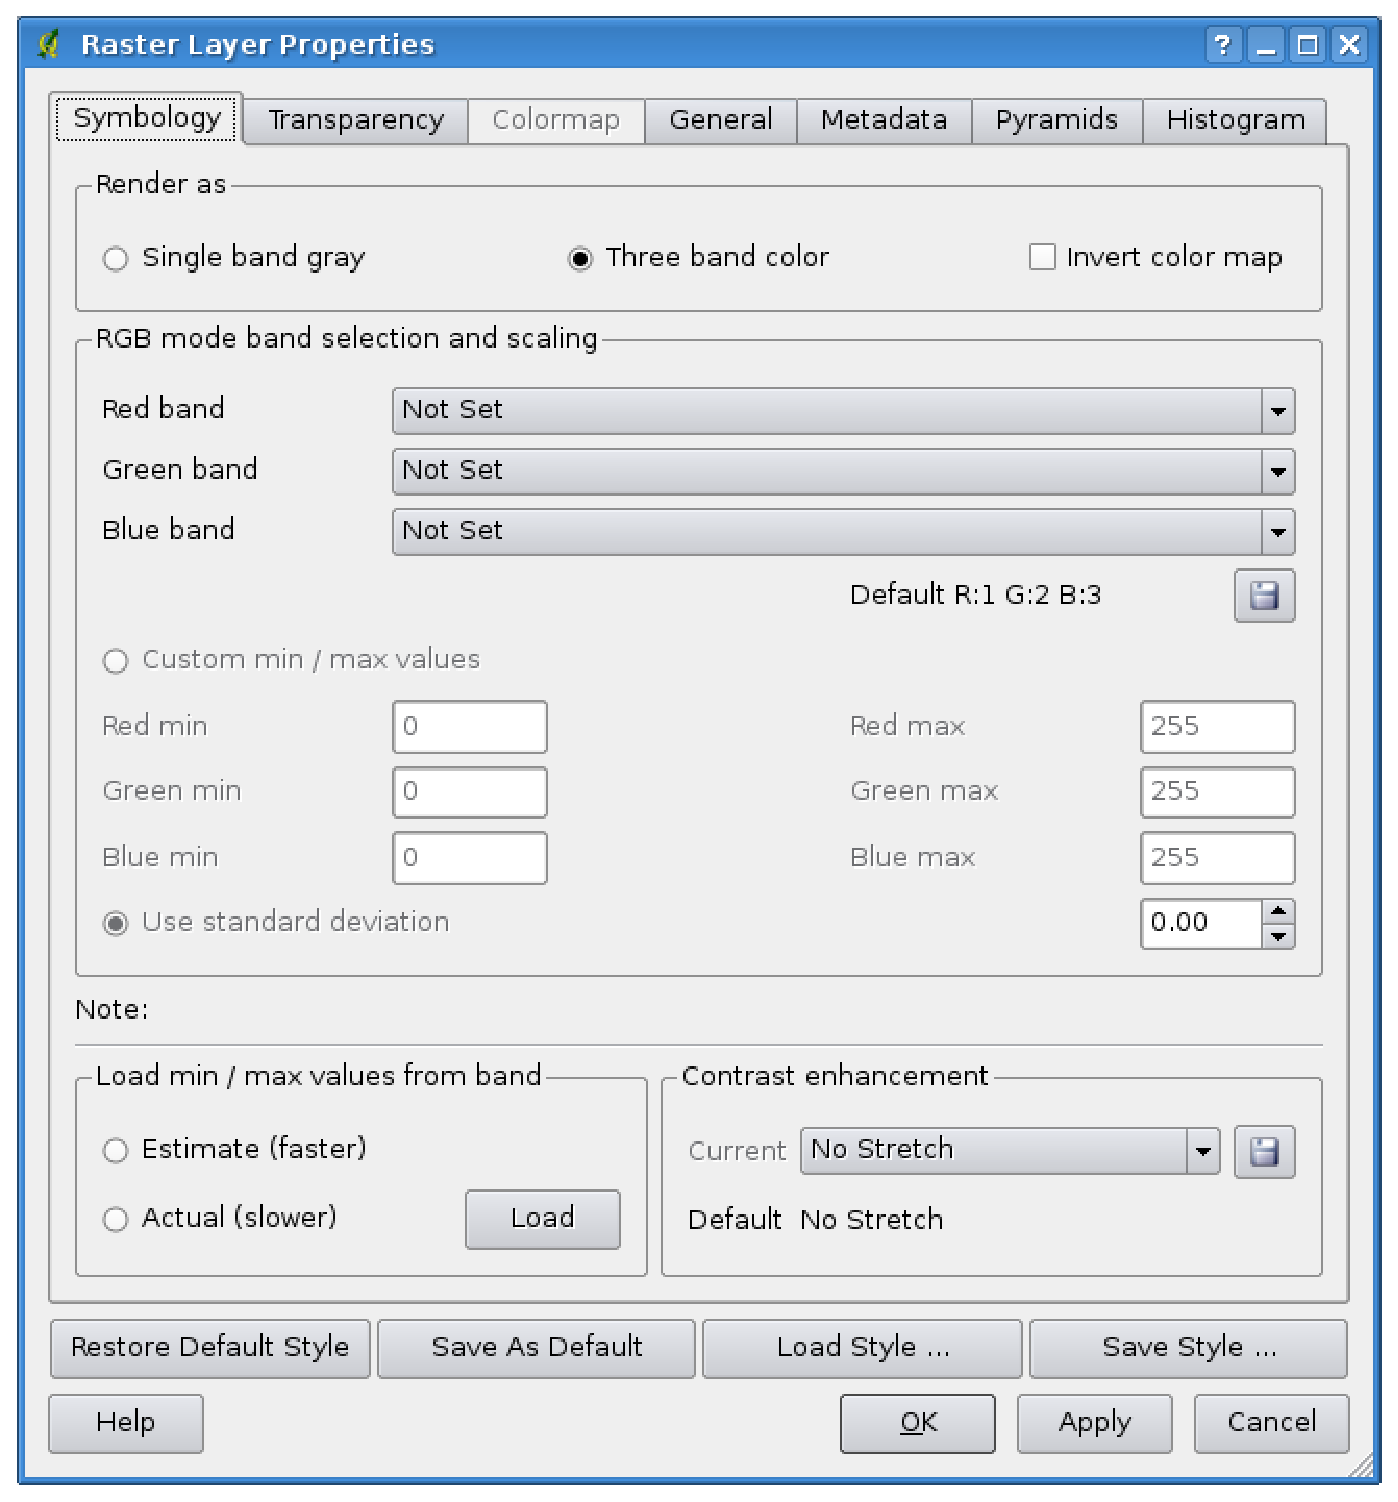
\includegraphics[clip=true, width=14cm]{rasterPropertiesDialog}
\end{center}
\end{figure}

\subsubsection{Onlget s\'emiologie}\label{label_sombology}

% QGIS can render raster layers in two different ways :\index{raster
% layers!supported channels}
QGIS peut afficher des couches raster de deux mani\`eres diff\'erentes
:\index{couches layers!canaux g\'er\'es}

\begin{itemize}
% \item Single band - one band of the image will be rendered as gray or in 
% pseudocolors.
\item Bande simple - une bande de l'image sera affich\'ee en nuance de gris ou en
pseudocouleurs.
% \item Three band color - three bands from the image will be rendered, each 
% band representing the red, green or blue component that will be used to
% create a color image.
\item Trois bandes de couleurs - trois bandes de l'image seront affich\'ees,
chaque bande repr\'esentant le composant rouge, vert ou bleu qui sera utilis\'e
pour cr\'eer une image de couleur.
\end{itemize}

% Within both rendertypes you can invert the color output using the 
% \checkbox{Invert color map} checkbox.
Pour les deux types de rendu vous pouvez inverser la sortie couleur en
utilisant la case \`a cocher \checkbox{Inverser la carte de couleur}

% \minisec{Single Band Rendering}
\minisec{Rendu des bandes simples}

% This selection offers you two possibilites to choose. At first you can
% select which band you like to use for rendering (if the dataset has more than 
% one band).
Ce choix vous permet deux possibilit\'es : vous pouvez d'abord s\'electionner
quelle bande vous voulez utiliser pour le rendu (si le jeu de donn\'ees a plus
d'une bande).

% The second option offers a selection of available colortables for rendering.
La seconde option vous offre une s\'election des tables de couleurs disponibles
pour le rendu.

% The following settings are available through the dropdownbox
% \selectstring{color map}{Grayscale}, where grayscale is the default setting.
Les param\`etres suivants sont disponibles \`a travers la liste d\'eroulante
\selectstring{carte de couleur}{Niveau de gris}, o\`u niveau de gris est le 
param\`etre par d\'efaut.

% Also available are
Sont aussi disponible :
\begin{itemize}
% \item Pseudocolor
\item Pseudo-couleur
% \item Freak Out
\item Pseudo-couleur psych\'ed\'elique
% \item Colormap
\item Couleurs index\'ees
\end{itemize}

% When selecting the entry \selectstring{color map}{Colormap}, the tab
% \tab{Colormap} becomes available. See more on that at chapter
% \ref{label_colormaptab}.
Quand vous s\'electionnez \selectstring{couleurs index\'ees}{Colormap}, l'onglet
\tab{Couleurs index\'ees} est disponible. Plus d'informations dans le chapitre
\ref{label_colormaptab}.

% QGIS can restrict the data displayed to only show cells whose values are
% within a given number of standard deviations of the mean for the
% layer.\index{raster layers!standard deviation} This is useful when you have
% one or two cells with abnormally high values in a raster grid that are having
% a negative impact on the rendering of the raster. This option is only
% available for pseudocolor images.
QGIS peut restreindre les donn\'ees affich\'ees pour afficher seulement les
cellules dont la valeur sont dans un nombre donn\'e de d\'eviations standards de
la moyenne pour la couche.\index{couches raster!d\'eviation standard} Cela est
utile quand vous avez une ou deux cellules avec des valeurs anormalement hautes
dans une grille raster qui ont un impact n\'egatif sur le rendu du raster. Cette
option est seulement disponible pour les images en pseudo-couleur.

% \minisec{Three band color}
\minisec{Couleur \`a trois bandes}

% This selection offers you a wide range of options to modify the appereance
% of your rasterlayer. For example you could switch color-bands from the
% standard RGB-order to something else.
Cette s\'election vous offre un large choix d'options pour modifier l'apparence
de votre couche raster. Par exemple, vous pouvez passer les bandes de couleurs
d'un ordre standard RVB \`a un autre.

% Also scaling of colors are available.
L'\'echantillonage des couleurs est \'egalement disponible.

% \begin{Tip}\caption{\textsc{Viewing a Single Band of a Multiband Raster}}
\begin{Tip}\caption{\textsc{Visualiser une seule bande d'un raster
multibande}
% \qgistip{If you want to view a single band (for example Red) of a multiband
% image, you might think you would set the Green and Blue bands to ``Not
% Set''. But this is not the correct way. To display the Red band, 
% set the image type to grayscale, then select Red as the band to use for Gray.
\qgistip{Si vous d\'esirez visualiser une seule bande (par exemple la bande rouge)
d'une image multibande, vous pouvez penser que vous pourriez d\'efinir les bandes
Vertes et Bleue \`a ``Non d\'efinie''. Mais ce n'est pas la mani\`ere correcte. Pour
afficher la bande Rouge d\'efinissez le type d'image \`a nuance de gris, puis
s\'electionnez Rouge comme bande \`a utiliser pour le Gris.
}
\end{Tip} 

% \subsubsection{Transparency Tab} \label{rastertab:transparency}
\subsubsection{Onglet transparence} \label{rastertab:transparency}

% QGIS has the ability to display each raster layer at varying transparency
% levels.\index{raster layers!transparency} Use the transparency slider to
% indicate to what extent the underlying layers (if any) should be visible
% though the current raster layer. This is very useful, if you like to overlay
% more than one rasterlayer, e.g. a shaded relief-map overlayed by a classified
% rastermap. This will make the look of the map more three dimensional.
QGIS a la possibilit\'e d'afficher chaque raster \`a des niveaux de transparence
diff\'erents.\index{couches raster!transparence} Utiliser la barre coulissante de
transparence pour indiquer \`a quel niveau de transparence les couches sous-jacentes
(s'il y en a) pourront \^etre visible \`a travers cette couche raster. Cela est
tr\`es utile, si vous d\'esirez superposer plus d'une couche raster, par exemple
une carte des reliefs ombr\'es superpos\'e par une carte raster classifi\'ee. Cela
rendra la carte encore plus proche de la 3e dimension.

% Additionally you can enter a rastervalue, which should be treated as
% {\em NODATA}.
De plus, vous pouvez entrer une valeur raster qui pourra \^etre trait\'e comme {\em
NODATA}

% An even more flexible way to customize the transparency can be done in the
% \guiheading{Custom transparency options} section.
% The transparency of every pixel can be set in this tab.
Un moyen encore plus flexible pour personnaliser la transparence est possible
dans la section \guiheading{Options de transparence personnalis\'ee}.
La transparence de chaque pixel peut \^etre d\'efinie dans cet onglet.

% As an example we want to set the water of our example rasterfile
% \filename{landcover.tif} to a transparency of 20\%. The following steps
% are neccessary:
Par exemple, nous voulons d\'efinir l'eau de notre fichier raster d'exemple
\filename{landcover.tif} \`a une transparence de 20 \%. Les \'etapes suivantes sont
n\'ecessaire :
\begin{enumerate}
%  \item  Load the rasterfile \filename{landcover}
\item Chargez le fichier raster \filename{landcover}
%  \item Open the \dialog{properties} dialog by double-clicking on the
%  rasterfile-name in the legend or by right-clicking and choosing
%  \dropmenuopt{Properties} from the popup meun.
 \item Ouvrez la bo\^ite de dialogue \dialog{propri\'et\'ees} en double-cliquant sur
le nom du raster dans la l\'egende ou avec un clic droit et en choisissant
\dropmenuopt{Propri\'et\'ees} du menu contextuel.
%  \item select the \tab{Transparency} tab
 \item S\'electionnez l'onglet \tab{Transparence}.
% \item \label{enum:add} Click the \toolbtntwo{mActionNewAttribute}{Add values
% manually} button. A new row will appear in the pixel-list.
  \item \label{enum:add} Cliquez sur le bouton
\toolbtntwo{mActionNewAttribute}{Ajouter des valeurs manuellement}. Une
nouvelle ligne apparait dans la liste des pixels.
%  \item \label{enum:transp} enter the the raster-value (we use 0 here) and
% adjust the  transparency to 20\%
 \item \label{enum:transp} Entrez la valeur du raster (nous utilisons 0 ici)
et ajustez la transparence \`a 20 \%.
%  \item press the \button{Apply} button and have a look at the map
 \item Pressez le bouton \button{Appliquer} et regardez la carte.
\end{enumerate}

% You can repeat the steps \ref{enum:add} and \ref{enum:transp} to adjust
% more values with custom transparency.
Vous pouvez r\'ep\'eter les \'etapes \ref{enum:add} et \ref{enum:transp} pour ajuster
d'autres valeurs avec une transparence personnalis\'ee. 

% As you can see this is quite easy set custom transparency, but it can be
% quite a lot of work. Therefor you can use the button
% \toolbtntwo{mActionFileSave}{Export to file} to save your transparency-list to
% a file. The button \toolbtntwo{mActionAddRasterLayer}{Import from file} loads
% your transparency-settings and applies them to the current rasterlayer.
Comme vous pouvez le voir il est assez facile de d\'efinir une transparence
personnalis\'ee, mais cela peut prendre un peu de temp. Par cons\'equent vous
pouvez utiliser le bouton \toolbtntwo{mActionFileSave}{Exporter dans un
fichier} pour sauver vos param\`etres  de transparence dans un fichier. Le
bouton \toolbtntwo{mActionAddRasterLayer}{Importer \`a partir d'un fichier} 
charge vos param\`etres de transparence et les applique \`a la couche raster actuel.

% \subsubsection{Colormap} \label{label_colormaptab}
 \subsubsection{Carte de couleur} \label{label_colormaptab}
% FIXME: Write me

% The \tab{Colormap} tab is only available, when you have selected a
% single-band-rendering within the tab \tab{Symbology} (see chapt.
% \ref{label_sombology}).
L'onglet \tab{Colormap} est seulement disponible quand vous avez s\'electionn\'e un
rendu \`a une seule bande dans l'onglet  \tab{S\'emiologie} (voir chapitre
\ref{label_sombology}).

% Three ways of color interpolation are available:
Trois mani\`eres de faire une interpolation de couleur sont disponibles :
\begin{itemize}
% \item Discrete
\item discr\`ete ;
% \item Linear
\item li\'enaire ;
% \item Exact
\item exacte.
\end{itemize}

% The button \button{Add Entry} adds a color to the individual color-table.
% Double-Clicking on the value-column lets you inserting a specific value.
% Double clicking on the color-column opens the dialog \dialog{Select
% color} where you can select a color to apply on that value.
Le bouton \button{Ajouter une entr\'ee} ajoute une couleur \`a la table de couleur
individuelle. Double-cliquez sur la colonne valeur vous permet d'ins\'erer une
valeur sp\'ecifique. Double-cliquez sur la colonne couleur ouvre une bo\^ite de
dialogue \dialog{S\'electionner une couleur}  o\`u vous pouvez s\'electionner une
couleur \`a appliquer sur cette valeur.

% Alternativly you can click on the button \toolbtntwo{mActionNewAttribute}{Load
% colormap from Band} , which tries to load the table from the band (if it has
% any).
Alternativement, vous pouvez cliquer sur le bouton
\toolbtntwo{mActionNewAttribute}{charger une carte de couleur \`a partir de
bande}  qui tente de charger la table \`a partir d'une bande (si celle-ci en a
une).

% The block \guiheading{Generate new color map} allows you to create newly
% categorized colormaps. You only need to select the \selectnumber{number of
% classes}{15} you need and press the button \button{Classify}. Currently
% only one \selectstring{Classification mode}{Equal Interval} is
% supported\index{raster layer!classify}.
Le bloc \guiheading{G\'en\`erer une nouvelle carte de couleurs} vous permet de
cr\'eer de nouvelles cartes de couleurs par cat\'egorie. Vosu avez seulement besoin
de s\'electionner le \selectnumber{nombre de classes}{15} dont vous avez besoin
et d'appuyez sur le bouton \button{Classifier}. Actuellement seule un 
\selectstring{mode de classification}{intervals \'egaux} est g\'er\'e\index{couches
raster!classifier}.

% \subsubsection{General Tab}\label{label_generaltab}
\subsubsection{Onglet g\'en\'eral}\label{label_generaltab}

% The \tab{General} tab displays basic information about the selected raster,
% including the layer source and  display name in the legend (which can be
% modified). This tab also shows a thumbnail of the layer, its legend symbol,
% and the palette.\index{raster layers!properties}
L'onglet \tab{G\'en\'eral} affiche des informations basiques sur le raster
s\'electionn\'e, incluant la source de la couche et le nom affich\'e dans la l\'egende
(qui peut \^etre modifi\'e). Cet onglet montre aussi un aper\c{c}u de la couche, le
symbol de la l\'egende, et la palette.\index{couches raster!propri\'et\'es}

% Additionally scale-dependent visability can be set in this tab. You need to
% check the checkbox and set an appropriate scale where your data will be
% displayed in the map canvas.
De plus la visibilit\'e en fonction de l'\'echelle peut \^etre d\'efinie dans cet
onglet. Vous devez activer la case \`a cocher et d\'efinir une \'echelle appropri\'ee \`a
laquelle vos donn\'ees seront affich\'ees dans la fen\^etre de la carte.

% Also the spatial reference system is printed here as a PROJ.4-string. This can
% be modified by hitting the \button{Change} button.
Le syst\`eme de r\'ef\'erence spatial est \'egalement affich\'e ici comme cha\^ine PROJ.4.
Cela peut \^etre modifi\'e en cliquant sur le bouton \button{Changer}.

% \subsubsection{Metadata Tab}\label{label_metatab}
\subsubsection{Onglet m\'eta-donn\'ees}\label{label_metatab}

% The \tab{Metadata} tab displays a wealth of information about the raster
% layer, including statistics about each band in the current raster layer.
% Statistics are gathered on a 'need to know' basis, so it may well be that a
% given layers statistics have not yet been collected.\index{raster
% layers!metadata}
L'onglet \tab{M\'eta-donn\'ees} affiche toute la richesse d'information sur la
couche raster, dont les statistiques sur chaque bande dans la couche raster
actuelle. Les statistiques sont recueillies sur l'id\'ee de la 'n\'ecessit\'e de
savoir', de sorte qu'il est possible qu'une couche n'ait pas de
statistique collect\'ee.\index{couches raster!m\'eta-donn\'ees} 

% This tab is mainly for information. You cannot change any values printed
% inside this tab. To update the statistics you need to change to tab
% \tab{Histogram} and press the button \button{Refresh} on the bottom right,
% see ch. \ref{label_histogram}.
Cet onglet est principalement pour informations. Vous ne pouvez pas modifier
les valeurs qui y sont affich\'ees. Pour mettre \`a jour les statistiques vous
devez aller dans l'onglet \tab{Histogramme} et pressez le bouton
\button{Rafraichir} en bas \`a droite, voir chapitre \ref{label_histogram}.

% \subsubsection{Pyramids Tab}\label{raster_pyramids}
\subsubsection{Onglet pyramides}\label{raster_pyramids}

% Large resolution raster layers can slow navigation in QGIS. By creating lower
% resolution copies of the data (pyramids), performance can be considerably
% improved as QGIS selects the most suitable resolution to use depending on the
% level of zoom.
Les couches raster \`a haute r\'esolution peuvent ralentir la navigation dans QGIS.
En cr\'eant des copies de plus basse r\'esolution des donn\'ees (pyramides), les
performances peuvent \^etre consid\'erablement am\'elior\'ees puisque QGIS s\'electionne
la r\'esolution la plus pertinente \`a utiliser en fonction du niveau de zoom.

% \index{raster layers!pyramids}
\index{couches raster!pyramides}
% \index{raster layers!resolution pyramids}
\index{couches raster!r\'esolution des pyramides}

% You must have write access in the directory where the original data is stored
% to build pyramids. \\
Vous devez avoir acc\`es en \'ecriture dans le r\'epertoire o\`u les donn\'ees
originelles sont stock\'ees pour construire les pyramides. \\
% Several resampling methods can be used to calculate the pyramides:
Plusieurs m\'ethodes de re\'echantillonage peuvent \^etre utilis\'ees pour calculer les
pyramides :
\begin{itemize}
% \item Average
\item moyen
% \item Nearest Neighbour
\item plus proche voisin ;
\end{itemize}

% When checking the checkbox \checkbox{Build pyramids internally if
% possible} QGIS tries to build pyramids internally.
Quand la case \checkbox{construire les pyramides en interne si possible} est
coch\'ee, QGIS tente de construire les pyramides en interne.

% Please note that building pyramids may alter the original data file and once
% created they cannot be removed. If you wish to preserve a 'non-pyramided'
% version of your raster, make a backup copy prior to building pyramids.
S'il vous plait notez que construire des pyramides peut alt\'erer les fichiers
donn\'ees originaux et une fois cr\'e\'e ils ne peuvent plus \^etre supprim\'e. Si vous
d\'esirez pr\'eserver une version 'sans pyramide' de vos raster, r\'ealisez une copie
de sauvegarde avant de les construire.

% \subsubsection{Histogram Tab}\label{label_histogram}
\subsubsection{Onglet histograme}\label{label_histogram}

% The \tab{Histogram} tab allows you to view the distribution\index{raster
% layers!histogram} of the bands or colors in your raster. You must first
% generate the raster statistics by clicking the \button{Refresh} button. You
% can choose which bands to display by selecting them in the list box at the
% bottom left of the tab. Two different chart types are allowed: 
L'onglet \tab{Histogramme}  vous permet de visualiser la distribution
\index{couches raster!histogramme} des bandes ou des couleurs dans votre
raster. Vous devez d'abord g\'en\'erer les statistiques du raster en cliquant le
bouton \button{Rafraichir}. Vous pouvez choisir quelles bandes \`a afficher en
les s\'electionnant dans la liste d\'eroulante en bas \`a gauche de l'onglet. Deux
types de graphiques diff\'erents sont permis :

\begin{itemize}
% \item Bar chart
\item graphique en barre ;
% \item Line graph
\item graphique lin\'eaire ;
\end{itemize}

% You can define the number of chart columns to use and decide wether you want 
% to \checkbox{Allow approximation} or display \checkbox{out of range} values 
% Once you view the histogram, you'll notice that the band statistics have been
% populated on the \tab{metadata} tab.\index{raster layers!metadata)}
Vous pouvez d\'efinir le nombre de colonnes du graphique \`a utiliser et d\'ecider si
vous voulez \checkbox{Permettre l'approximation} ou afficher les valeurs
\checkbox{En dehors du domaine}. Une fois que vous avez vu l'histogramme, vous
remarquerez que les statistiques des bandes ont \'et\'e remplies dans l'onglet
\tab{m\'eta-donn\'ees}.\index{couches raster!m\'eta-donn\'ees}

% \begin{Tip}\caption{\textsc{Gathering Raster Statistics}}
\begin{Tip}\caption{\textsc{Regroupement des statistiques raster}}
% \qgistip{To gather statistics for a layer, select pseudocolor rendering and
% click the \button{Apply} button. Gathering statistics for a layer can be time
% consuming. Please be patient while QGIS examines your
% data!\index{raster layers!statistics}
\qgistip{Rassembler des statistiques pour une couche, s\'electionnez un rendu en
pseudo-couleur et cliquez sur le bouton \button{Appliquer}. Regrouper des
statistiques pour une couche peut prendre du temp. Soyez patient pendant que
QGIS examine  vos donn\'ees !\index{couches raster!statistiques}
}
\end{Tip}

% vim: set textwidth=78 autoindent:

\section{Lavorare con dati OGC}

% when the revision of a section has been finalized, 
% comment out the following line:
%\updatedisclaimer

QGIS supporta sorgenti di dati WMS e WFS. Il supporto WMS è nativo, quello per
WFS è fornito tramite plugin.

\subsection{What is OGC Data}\index{OGC!introduction}

L'Open Geospatial Consortium (OGC), è un’organizzazione internazionale che raggruppa più
di 300 organizzazioni commerciali, governative, nonprofit e di ricerca.
I suoi membri sviluppano e implementano standards per contenuti e servizi geospaziali,
analisi GIS e scambio dati.

Dal Consorzio è stato quindi elaborato un numero crescente di specifiche per i modelli di
dati per garantire bisogni specifici riguardanti l'interoperabilità
nell'ambito della tecnologia geospaziale, inclusi i GIS. Ulteriori
informazioni all'indirizzo \url{http://www.opengeospatial.org/}.

Importanti specifiche OGC sono:

\begin{itemize}
\item \textbf{WMS} - Web Map Service
\item \textbf{WFS} - Web Feature Service
\item \textbf{WCS} - Web Coverage Service
\item \textbf{CAT} - Web Catalog Service
\item \textbf{SFS} - Simple Features for SQL
\item \textbf{GML} - Geography Markup Language
\end{itemize}

Ad oggi i servizi OGC-sono sempre più di uso comune per scambiare dati geografici fra
differenti implementazioni GIS. QGIS ora può gestire tre delle specifiche esposte sopra
tra cui SFS (tramite il supporto a PostgreSQL/PostGIS, vedi Sezione
\ref{label_postgis}); e WFS e WMS come client.


\subsection{Client WMS}\label{sec:ogc-wms}\index{WMS!client}\index{OGC!WMS!client}\index{rasters!WMS}

\subsubsection{Panoramica sul servizio WMS}\label{sec:ogc-wms-about}\index{WMS!client!about}

QGIS può agire come client WMS, nel rispetto delle specifiche 1.1, 1.1.1 e 1.3.
E’ stato particolarmente testato nei confronti di server accessibili pubblicamente
quali DEMIS e JPL OnEarth.

I server WMS rispondono alle richieste da parte dei clients (ad es. QGIS) di una mappa raster
di una determinata estensione, con un determinato insieme di strati, simboli e trasparenza.
Il server WMS quindi consulta le sue risorse (locali o remote), genera il raster e lo invia
al client in formato raster, per QGIS tipicamente come immagini JPEG o PNG.

WMS è un servizio REST (Representational State Transfer) piuttosto che un servizio web completo.
Come tale, si può prendere la URL (indirizzo del server con specifiche) generata da QGIS e usarla
in un browser web per ottenere la stessa immagine che QGIS usa internamente. Questo può essere
utile per identificare le cause di eventuali problemi, dato che esistono vari tipi di server
WMS e ciascuno ha la sua propria interpretazione degli standards WMS.

Gli strati WMS possono essere aggiunti molto semplicemente, una volta
disponibile l'indirizzo (URL) per accedere al server WMS, una connessione adatta
e posto che il server usi l’HTTP come meccanismo di trasferimento dati.

\subsubsection{Scegliere un server WMS}\label{sec:ogc-wms-servers}\index{WMS!remote server!selection}

La prima volta in cui si vuole utilizzare un servizio WMS, non sono presenti
server predefiniti. Si può avviare lo strumento cliccando sul pulsante
\toolbtntwo{mActionAddWmsLayer}{Aggiungi layer WNS} nella barra strumenti, 
oppure dalla voce di menù
\mainmenuopt{Layer}>\dropmenuopttwo{mActionAddWmsLayer}{Aggiungi layer WMS...}.
Si aprirà la finestra di dialogo \dialog{Aggiungi layer dal server}. È
possibile aggiungere alcuni servers cliccando sul pulsante
\button{Aggiungi server predefiniti}. Verranno quindi aggiunti almeno tre
servers WMS, incluso il server della NASA (JPL). Per definire un nuovo server WMS
nella sezione \tab{Connessioni server}, cliccare su \button{Nuovo} ed inserire
i parametri di connessione al server WMS desiderato, seguendo le indicazioni della
tabella \ref{tab:wms_connection_parms}:

\begin{table}[ht]\index{WMS!client!connection parameters}
\centering
\caption{Parametri del collegamento WMS}\label{tab:wms_connection_parms}\medskip
 \begin{tabular}{|l|p{5in}|}
\hline Nome & nome per la connessione che consenta di individuarlo nella
lista dei server WNS nel menù a tendina. \\
\hline URL \index{WMS!URL} &  indirizzo URL del server che fornisce i dati.
Deve essere un indirizzo raggiungibile, nello stesso formato che verrebbe
usato per aprire una connessione telnet o pingare un host. \\
\hline
\end{tabular}
\end{table}

È possibile, se necessario, impostare nelle opzioni i parametri del proxy per ricevere i servizi WMS da internet.
Selezionare la voce di menù \mainmenuopt{Impostazioni} >
\dropmenuopttwo{mActionOptions}{Opzioni} e cliccare sulla linguetta
\tab{Proxy}, nella quale è possibile inserire le impostazioni abilitando la
casella di controllo \checkbox{Utilizza un proxy per l'accesso web}.

Una volta creata la connessione al server WMS, essa sarà memorizzata e
disponibile per le successive sessioni di QGIS.

\begin{Tip}[ht]\caption{\textsc{A proposito di indirizzi dei server WMS}}
\qgistip{Quando si inserisce l'indirizzo del server URL, assicurarsi di
inserire l'indirizzo di base. Ad esempio non bisogna inserire frammenti tipo
\usertext{request=GetCapabilities} o \usertext{version=1.0.0} nell'indirizzo.\index{WMS!remote server!URL}
}
\end{Tip}

La tabella \ref{tab:wms_example_urls} mostra alcuni esempi di indirizzi di
server WMS con i quali iniziare.
Questi links sono stati controllati l'ultima volta nel Dicembre 2006, ma
potrebbere essere nel frattempo essere stati modificati:

%FIXME:  WMS URLs should be checked again and maybe extended in QGIS 

\begin{table}[ht]\index{WMS!remote server!URL!examples}
\centering
\caption{Esempi di indirizzi di server WMS pubblici}\label{tab:wms_example_urls}\medskip
 \begin{tabular}{|l|l|}
\hline \textbf{Name}        & \textbf{URL} \\
\hline Atlas of Canada      & http://atlas.gc.ca/cgi-bin/atlaswms\_en? \\
\hline DEMIS                & http://www2.demis.nl/wms/wms.asp?wms=WorldMap\& \\
\hline Geoscience Australia & http://www.ga.gov.au/bin/getmap.pl?dataset=national \\
\hline NASA JPL OnEarth     & http://wms.jpl.nasa.gov/wms.cgi? \\
\hline QGIS Users           & http://qgis.org/cgi-bin/mapserv?map=/var/www/maps/main.map\& \\
\hline
\end{tabular}
\end{table}

Un elenco esaustivi di servers WMS è reperibile all'indirizzo \url{http://wms-sites.com}.

\subsubsection{Caricare livelli WMS}\label{sec:ogc-wms-layers}\index{WMS!client!layers}

Una volta compilati correttamente i campi, si può premere sul pulsante
\button{Connetti} per ottenere le capacità del server. Tra queste sono inclusi
i formati immagine, i layer disponibili e i sistemi di proiezione forniti dal
server. Considerato che si tratta di operazioni in rete, la velocità nella
risposta dipenderà dalla qualità della connessione verso il server WMS. Mentre
si scaricano i dati dal server, l'avanzamento dell'operazione viene
visualizzato nella porzione inferiore sinistra della finestra. 

Lo schermo dovrebbe rassomigliare alla Figura \ref{fig:connection_wms}, che
mostra la risposta fornita dal server WMS NASA JPL OnEarth.

\begin{figure}[ht]
  \begin{center}
  	\caption{Finestra per l'aggiunta di un server WMS, nella quale vengono
	mostati gli strati disponibili \nixcaption}\label{fig:connection_wms}
	\includegraphics[clip=true,width=0.6\textwidth]{connection_wms}
  \end{center}
\end{figure}

\minisec{Codifica immagine}

La sezione \tab{Codifica immagine} elenca i formati supportati sia dal client
che dal  server. La scelta dipenderà dalla risoluzione che necessita allo scopo
prefisso.

\begin{Tip}[ht]\caption{\textsc{Codifica immagine}}
\qgistip{Solitamente un server WMS offrirà la scelta tra le codifiche JPEG e
PNG. Mentre la compressione JPEG comporta una perdita di qualità, quella PNG
riproduce fedelmente il dato di origine. Usare JPEG se non interessa avere una
certa perdita di qualità dell'immagine, riducendo d'altro canto il tempo per
il download dei dati di 5 volte rispetto al formato PNG. Usare invece PNG se
si vuole una rappresentazione precisa del dato originale e non ci si preoccupa
del tempo necessario per il trasferimento dei dati.
\index{WMS!image encoding}
}
\end{Tip}

\minisec{Layers}

La sezione \tab{Layer} elenca i livelli disponibili dal server WMS
selezionato. Si vedrà che alcuni layers sono espandibili, il che comporta che
essi possono essere mostrati in diversi stili di immagine.

Possono essere selezionati diversi layers alla volta, ma un solo stile di
immagine per ognuno di essi. Quando si effettua una selezione multipla, i
livelli vengono richiesti al server e trasmessi a QGIS in un solo blocco.

\begin{Tip}[ht]\caption{\textsc{Ordine degli strati WMS}}
\qgistip{In questa versione di QGIS, i layers WMS caricati sono sovrapposti in
base all'ordine in cui sono elencati nella sezione Layer, dall'alto verso il
basso. Se si desidera sovrapporre gli strati nel senso opposto occorre
selezionare una seconda volta \toolbtntwo{mActionAddWmsLayer}{Aggiungi layer
WMS}, scegliere nuovamente lo stesso server e selezionare il secondo gruppo di
strati che si desidera sovrapporre al primo.
\index{WMS!remote server!layer ordering}
}
\end{Tip}

\minisec{Trasparenza}\label{ogc-wms-transparency}

In questa versione di QGIS la trasparenza è impostata per essere sempre
attiva, se disponibile.

\begin{Tip}[ht]\caption{\textsc{Trasparenza dei Layer WMS}}
\qgistip{La possibilità di rendere trasparenti gli strati WMS dipenda dalla codifica tramite la quale sono stati caricati: PNG e GIF gestiscono la trasparenza mentre il JPEG no.
\index{WMS!layer transparency}
}
\end{Tip}

\minisec{Coordinate Reference System}
\index{WMS!CRS}\index{WMS!coordinate reference system}
\index{OGC!CRS}\index{OGC!coordinate reference system}
\index{Projections!WMS}
\index{Projections!CRS}\index{Projections!coordinate reference system}
\index{CRS}\index{coordinate reference system}
\index{SRS}\index{Projections!SRS}

A Coordinate Reference System (CRS) is the OGC terminology for a QGIS Projection.

Each WMS Layer can be presented in multiple CRSs, depending
on the capability of the WMS server.  You may notice that the \textsl{x} changes in
the \textsl{Coordinate Reference System (x available)} header as you
select and deselect layers from the \tab{Layers} section.

To choose a CRS, select \button{Change...} and a screen similar to
Figure \ref{fig:projections} in Section \ref{label_projstart} will appear.
The main difference with the WMS version of the screen is that only
those CRSs supported by the WMS Server will be shown.


\begin{Tip}[ht]\caption{\textsc{WMS Projections}}
\qgistip{For best results, make the WMS layer the first layer
you add in the project.  This allows the project
projection to inherit the CRS you used to render the WMS layer.
On-the-fly projection (see Section \ref{sec:projection-specifying})
can then be used to fit any subsequent
vector layers to the project projection.
In this version of QGIS, if you add a WMS layer later, and give it a different
CRS to the current project projection, unpredictable
results can occur.
}
\end{Tip}


\subsubsection{Using the Identify Tool}\label{sec:ogc-wms-identify}
\index{WMS!identify}
\index{identify!WMS}
\index{WMS!GetFeatureInfo}

Once you have added a WMS server, 
and if any layer from a WMS server is queryable, you can then use
the \toolbtntwo{mActionIdentify}{Identify} tool to select a pixel on the map canvas.
A query is made to the WMS server for each selection made.

The results of the query are returned in plain text.
The formatting of this text is dependent on the particular
WMS server used.

% FIXME: GetFeatureInfo-Requests are done here?

\subsubsection{Viewing Properties}\label{sec:ogc-wms-properties}\index{WMS!properties}
\index{rasters!properties}

Once you have added a WMS server, you can view its properties
by right-clicking on it in the legend, and selecting
\button{Properties}.


\minisec{Metadata Tab}\label{sec:ogc-wms-properties-metadata}
\index{rasters!metadata}
\index{WMS!metadata}
\index{WMS!capabilites}

The \tab{Metadata} tab displays a wealth of information about the WMS server,
generally collected from the Capabilities statement returned from
that server.

Many definitions can be gleaned by reading the WMS
standards \cite{OGCWMS010101web}, \cite{OGCWMS010300web}, but
here are a few handy definitions:

\begin{itemize}
\item \textbf{Server Properties}

\begin{itemize}
\item \textbf{WMS Version}      - The WMS version supported by the server.

\item \textbf{Image Formats}    - The list of MIME-types the server can respond with when
                                  drawing the map.  QGIS supports whatever formats
                                  the underlying Qt libraries were built with, which
                                  is typically at least \texttt{image/png} 
                                  and \texttt{image/jpeg}.

\item \textbf{Identity Formats} - The list of MIME-types the server can respond with when
                                  you use the Identify tool.  Currently QGIS supports
                                  the \texttt{text-plain} type.

\end{itemize}

\item \textbf{Layer Properties}

\begin{itemize}
\item \textbf{Selected}         - Whether or not this layer was selected when its                                                                        server was added to this project.

\item \textbf{Visible}          - Whether or not this layer is selected as visible
                                  in the legend.  (Not yet used in this version of QGIS.)

\item \textbf{Can Identify}     - Whether or not this layer will return any results
                                  when the Identify tool is used on it.

\item \textbf{Can be Transparent} - Whether or not this layer can be rendered with transparency.
                                    This version of 
                                    QGIS will always use transparency if this is \textsl{Yes}
                                    and the image encoding supports transparency
% BM: doesn't seem to work?
%                                    (see Section
%                                    \ref{ogc-wms-transparency}
%                                    ).
                                    .

\item \textbf{Can Zoom In}      - Whether or not this layer can be zoomed in by the server.  This version
                                  of QGIS assumes all WMS layers have this set to \textsl{Yes}.
                                  Deficient layers may be rendered strangely.

\item \textbf{Cascade Count}    - WMS servers can act as a proxy to other WMS servers to get
                                  the raster data for a layer.  This entry shows how
                                  many times the request for this layer is forwarded to peer
                                  WMS servers for a result.

\item \textbf{Fixed Width}, \textbf{Fixed Height}
                                - Whether or not this layer has fixed source pixel dimensions.
                                  This version
                                  of QGIS assumes all WMS layers have this set to nothing.
                                  Deficient layers may be rendered strangely.

\item \textbf{WGS 84 Bounding Box} - The bounding box of the layer, in WGS 84 coordinates.
                                     Some WMS servers do not set this correctly (e.g. UTM
                                     coordinates are used instead).  If this is the case,
                                     then the initial view of this layer may be rendered
                                     with a very ``zoomed-out'' appearance by QGIS.
                                     The WMS webmaster should be informed of this error,
                                     which they may know as the WMS XML elements
                                     \texttt{LatLonBoundingBox},
                                     \texttt{EX\_GeographicBoundingBox} or
                                     the CRS:84 \texttt{BoundingBox}.

\item \textbf{Available in CRS} - The projections that this layer can be rendered in by
                                  the WMS server.  These are listed in the WMS-native format.

\item \textbf{Available in style} - The image styles that this layer can be rendered in by
                                    the WMS server.

\end{itemize}

\end{itemize}


\subsubsection{WMS Client Limitations}\label{sec:ogc-wms-limits}\index{WMS!client!limits}

Not all possible WMS Client functionality had been included in this version of QGIS.
Some of the more notable exceptions follow:

\minisec{Editing WMS Layer Settings}
\index{WMS!layer settings!editing}

Once you've completed the \toolbtntwo{mActionAddWmsLayer}{Add WMS layer}
procedure, there is no ability to change the settings.

A workaround is to delete the layer completely and start again.

\minisec{WMS Servers Requiring Authentication}
\index{WMS!remote server!authentication}

Only public WMS servers are accessible.
There is no ability to apply a user name and password combination
as an authentication to the WMS server.

\begin{Tip}[ht]\caption{\textsc{Accessing secured OGC-layers}}
\qgistip{If you need to access secured layers, you could use InteProxy as
a transparent proxy, which does supports several authentification methods.
More information can be found at the InteProxy-manual found on the website
\url{http://inteproxy.wald.intevation.org}.
\index{WMS!secured layers!}\index{OGC!Authentication}
}
\end{Tip}


\subsection{WFS Client}

In QGIS, a WFS layer behaves pretty much like any other vector layer. You 
can identify and select features and view the attribute table. An exception 
is that editing is not supported at this time. To start the WFS plugin you 
need to open \mainmenuopt{Plugins} > \dropmenuopttwo{mActionShowPluginManager}{Plugin Manager...}, 
activate the \checkbox{WFS plugin} checkbox and click \button{OK}. 

A new \toolbtntwo{mIconAddWfsLayer}{Add WFS Layer} icon appears next 
to the WMS icon. Click on it to open the dialog. In General adding a WFS 
layer is very similar to the procedure used with WMS. The difference is 
there are no default servers defined, so we have to add our own.

\subsubsection{Loading a WFS Layer}

As an example we use the DM Solutions WFS server and display a layer. The URL is:
\begin{verbatim}
http://www2.dmsolutions.ca/cgi-bin/mswfs_gmap?VERSION=1.0.0&SERVICE=
wfs&REQUEST=GetCapabilities
\end{verbatim}

\begin{enumerate}
  \item Make sure the WFS plugin is loaded; if not, open the Plugin Manager and load it
  \item Click on the 
  \toolbtntwo{mIconAddWfsLayer}{Add WFS Layer} 
  tool on the plugins toolbar
  \item Click on \button{New} 
  \item Enter \inputtext{Name}{DM Solutions} as the name
  \item Enter the URL (see previous page)
  \item Click \button{OK} 
  \item Choose \selectstring{Server Connections}{DM Solutions} from the drop-down box
  \item Click \button{Connect} 
  \item Wait for the list of layers to be populated
  \item Click on the \clicklistitem{Canadian Land} layer
  \item Click \button{Add} to add the layer to the map
  \item Wait patiently for the features to appear
\end{enumerate}

\begin{figure}[ht]
  \begin{center}
  	\caption{Adding a WFS layer \nixcaption}\label{fig:wfs_dmsolutions}
	\includegraphics[clip=true,width=0.6\textwidth]{connection_wfs}
  \end{center}
\end{figure}

You'll notice the download progress is visualized in the left bottom of the QGIS main window. 
Once the layer is loaded, you can identify and select a province or two and view the 
attribute table.

Remember this plugin works best with UMN MapServer WFS servers. It still
could be, that you might experience random behavior 
and crashes. You can look forward to improvements in a future version of the plugin.

\begin{Tip}[ht]\caption{\textsc{Finding WMS and WFS Servers}}
\qgistip{You can find additional WMS and WFS servers by using Google or your
favorite search engine. There are a number of lists with public URLs, some 
of them maintained and some not.
\index{WFS!remote server!}
}
\end{Tip} 


% vim:autoindent:set textwidth=78:

\section{Arbeiten mit Projektionen}\label{label_projections}
\index{Koordinatenbezugssystem}\index{Projektion}

% when the revision of a section has been finalized, 
% comment out the following line:
%\updatedisclaimer

QGIS erm�glicht es, globale und projektbezogene KBS (Koordinatenbezugssysteme)
f�r Layer ohne vordefinierte KBS zu definieren. Es k�nnen benutzerdefinierte
Koordinatenbezugssysteme erstellt werden und f�r Vektorlayer wird On-The-Fly
(OTF) Projektion unterst�tzt, um Layer gemeinsam und lagegenau darzustellen,
obwohl sie unterschiedliche KBS besitzen. 

\subsection{�berblick zur Projektionsunterst�tzung}\label{label_projoverview}

QGIS unterst�tzt etwa 2700 bekannte Koordinatenbezugssysteme (KBS). Diese
sind in einer SQlite-Datenbank abgelegt, die mit QGIS installiert wird.
Normalerweise muss diese Datenbank nicht editiert werden, und es kann
Probleme verursachen, wenn Sie es dennoch versuchen. Selbst definierte KBS
sind in einer Benutzerdatenbank abgelegt. Informationen zum Anlegen einer
Benutzerdatenbank finden Sie im Abschnitt \ref{sec:customprojections}.

Die Koordinatenbezugssysteme in QGIS basieren auf EPSG Codes\index{EPSG} und
sind weitestgehend der spatial\_references Tabelle von PostGIS\index{PostGIS}
Version 1.x entnommen. Wichtig ist, dass die IDs, welche von QGIS benutzt
werden, nicht den IDs der spatial\_references Tabelle oder den EPSG Codes
entsprechen. Die EPSG und PostGIS IDs sind in der SQlite-Datenbank abgelegt
und werden benutzt, um KBS in QGIS zu spezifizieren.

Um OTF Projektion zu verwenden, m�ssen die Daten Informationen �ber ihr
Koordinatenbezugssystem enthalten. Bei PostGIS-Layern benutzt QGIS die spatial
reference ID, die bei der Erstellung des Layers festgelegt wurde. Bei Daten,
die von der OGR-Bibliothek unterst�tzt werden, bezieht sich QGIS auf das
Vorhandensein eines KBS bei den Daten. Bei Shapes bedeutet dies, dass eine
Datei mit der Endung .prj vorhanden sein muss, in der das KBS im Well
Known Text (WKT)\index{WKT} Format angegeben ist. F�r ein Shape mit dem Namen
\filename{lakes.shp} g�be es also eine entsprechende Projektionsdatei
\filename{lakes.prj}. 

\subsection{Ein Koordinatenbezugssystem festlegen}
\index{Koordinatenbezugssystem!festlegen}
\label{sec:projection-specifying}

QGIS setzt das Koordinatenbezugssystem beim Start nicht mehr automatisch auf
das KBS des zuerst geladenen Layers. Wenn Sie QGIS mit einem Layer starten,
der keine KBS-Informationen bereitstellt, m�ssen Sie f�r diesen Layer ein
KBS festlegen. Dies kann global oder projektbezogen im Reiter \tab{KBS} im
Men� \mainmenuopt{Einstellungen} > \dropmenuopttwo{mActionOptions}{Optionen}
geschehen (Siehe Abbildung~\ref{fig:crsdialog}) 

\begin{itemize}
\item \checkbox{KBS abfragen} 
\item \checkbox{Projektweite KBS-Voreinstellung}
\item \checkbox{Untenstehende globale Voreinstellung wird genutzt}
\end{itemize}

Das globale standard Koordinatenbezugssystem \usertext{proj=longlat
+ellps=WGS84 +datum=WGS84 +no\_defs} ist vordefiniert in QGIS, kann aber
nat�rlich ge�ndert werden und wird dann f�r folgende Sitzungen gespeichert. 

\begin{figure}[ht]
   \begin{center}
   \caption{KBS Reiter im Dialog Optionen \nixcaption}\label{fig:crsdialog}\smallskip
   \includegraphics[clip=true, width=11cm]{crsdialog}
\end{center}
\end{figure}

Wenn Sie ein Koordinatenbezugssystem f�r einen bestimmten Layer festlegen
m�chten, k�nnen Sie das im Reiter \tab{Allgemein} der Dialoge f�r 
Rasterlayereigenschaften (\ref{label_generaltab}) und
Vektorlayereigenschaften (\ref{vectorgeneraltab}) machen. Falls der geladene
Layer bereits Informationen zu seinem Koordinatenbezugssystem enth�lt,
werden diese angezeigt (siehe Abbildung~\ref{fig:vector_symbology}).

\subsection{On-The-Fly (OTF) Projektion}\label{label_projstart}

In QGIS ist die Unterst�tzung f�r On-The-Fly (OTF) Projektion nicht als
Standard aktiviert. Um diese auszuw�hlen, �ffnen Sie den Dialog
\dropmenuopttwo{mActionOptions}{Projekteinstellungen}, wechseln in den Reiter
\tab{Benutzerkoordinatenreferenzsystem} und klicken dort auf das
Kontrollk�stchen \checkbox{On-The-Fly-KBS-Transformation aktivieren}. 

Um den Dialog \tab{Benutzerkoordinatenreferenzsystem} zu �ffnen, k�nnen Sie
auch auf das Icon \toolbtntwo{mIconProjectionEnabled}{KBS-Status} in der
unteren rechten Ecke der Statusleiste dr�cken.

Wenn Sie bereits einen Layer geladen haben und nun die Unterst�tzung f�r
On-The-Fly (OTF) Projektion aktivieren wollen ist der beste Weg folgender.
�ffnen Sie den Reiter \tab{Benutzerkoordinatenreferenzsystem} im Men�
\dropmenuopttwo{mActionOptions}{Projekteinstellungen}, w�hlen Sie das
passende KBS f�r den Layer aus und aktivieren Sie dann das
Kontrollk�stchen \checkbox{On-The-Fly-KBS-Transformation aktivieren}. Alle
daraufhin geladenen Vektorlayer werden werden dann On-The-Fly auf das
ausgew�hlte KBS projiziert. 

Der Reiter \tab{Benutzerkoordinatenreferenzsystem} enth�lt vier wichtige
Optionen (siehe Abbildung~\ref{fig:projections}). Diese werden im Folgenden
beschrieben.

\begin{figure}[ht]
   \begin{center}
   \caption{Dialog Projekteinstellungen \nixcaption}\label{fig:projections}\smallskip
   \includegraphics[clip=true, width=11cm]{projectionDialog}
\end{center}  
\end{figure}

\begin{enumerate}
\item \textbf{On-The-Fly-KBS-Transformation
aktivieren}\index{Koordinatenbezugssystem!OTF!aktivieren} 
- �ber diese Checkbox wird die OTF Projektion aktiviert oder deaktiviert.
  Wenn sie deaktiviert ist, wird jeder Layer entsprechend seines KBS
  dargestellt. Wenn es aktiviert ist, wird jeder Layer beim Laden in die
definierte Koordinatenbezugssystem 'on-the-fly' umgewandelt dargestellt.
\item \textbf{Koordinatensystem} - dies ist eine Liste mit allen
Koordinatenbezugssystemen, die von QGIS unterst�tzt werden. Um ein
KBS zu benutzen, w�hlt man es aus der Liste aus. Die bis dahin aktive
Projektion ist vorgegeben als WGS 84.
\item \textbf{Proj4 Text} - dies ist ein Ausdruck, der von der PROJ-Bibliothek
genutzt wird. Es dient nur zur Information und kann nicht ver�ndert werden.
\item \textbf{Suchen} - wenn Sie den EPSG Code oder den Namen f�r ein KBS
kennen, k�nnen Sie diese benutzen, um ihr Koordinatenbezugssystem zu finden.
Geben Sie eine ID  der Namen ein und klicken Sie auf \button{Finden}.
\end{enumerate}

\begin{Tip}
\caption{\textsc{Dialog Projekteigenschaften}}
\qgistip{Wenn Sie den Dialog \dialog{Projekteigenschaften} �ber die
Men�leiste �ffnen, m�ssen Sie erst auf den Reiter
\tab{Benutzerkoordinatenreferenzsystem} dr�cken. �ber das
\toolbtntwo{mIconProjectionEnabled}{KBS-Status} Icon in der Statusleiste
unten rechts wird der Reiter \tab{Benutzerkoordinatenreferenzsystem} direkt
in den Vordergrund ger�ckt.
}
\end{Tip}

\subsection{Ein Koordinatenbezugssystem selbst definieren}\label{sec:customprojections}
\index{Koordinatenbezugssystem!anpassen}

Wenn QGIS nicht das KBS bereith�lt, welches Sie brauchen, k�nnen Sie ein
eigenes KBS erstellen. Dazu w�hlen Sie in der Men�leiste
\mainmenuopt{Einstellungen} >
\dropmenuopttwo{mIconNew}{Benutzerkoordinatenbezugssystem}. Das eigene KBS
wird in einer Benutzerdatenbank erstellt. Diese enth�lt Ihre r�umlichen
Lesezeichen und die selbst erstellten Projektionen.

\begin{figure}[ht]
   \begin{center}
   \caption{Definition eines eigenen Koordinatenbezugssystems \nixcaption}\label{fig:customprojections}\smallskip
   \includegraphics[clip=true, width=11cm]{customProjectionDialog}
\end{center}  
\end{figure}

In QGIS bedarf es einem grundlegenden Verst�ndnis im Umgang mit der
PROJ4-Bibliothek. Zu Beginn sollten Sie einen Blick in das Benutzerhandbuch
von PROJ werfen. Cartographic Projection Procedures for the UNIX Environment
- A User's Manual by Gerald I. Evenden, U.S. Geological Survey Open-File Report
90-284, 1990 (zu finden unter \url{ftp://ftp.remotesensing.org/proj/OF90-284.pdf}).
Dieses Handbuch beschreibt die Anwendung von \usertext{proj.4}. Die dort
beschriebenen kartographischen Parameter sind identisch mit denen, die in QGIS
verwendet werden.

Der Dialog \dialog{Definition eines Benutzerkoordinatenbezugssystem} braucht
nur zwei Eintr�ge, um eine eigene Projektion zu definieren:

\begin{enumerate}
\item Einen Namen
\item kartographische Parameter 
\end{enumerate}

Um ein neues KBS zu erstellen, klicken Sie auf den Knopf
\toolbtntwo{mIconNew}{Neu}, geben Sie einen beschreibenden Namen ein
und die kartographischen Parameter. Abbildung \ref{fig:customprojections}
zeigt den Dialog mit einer Beispielprojektion. Danach speichern Sie das neue
KBS mit dem Knopf \toolbtntwo{mActionFileSave}{Speichern} ab. 

Denken Sie daran, dass die kartographischen Parameter mit einem
\usertext{+proj=}-Block beginnen m�ssen, um den Beginn eines neuen KBS
anzuzeigen. 

Sie k�nnen das neue KBS testen, um zu sehen, ob bei einer Konvertierung
von bekannten WGS84 Lat-Lon Koordinaten in ihre Projektion ein sinnvolles
Ergebnis herauskommt. Dazu kopieren Sie ihre kartographischen Parameter in
das Fenster \guilabel{Parameter}, geben ein paar bekannte WGS84 Lat-Lon
Koordinaten an und klicken dann auf den Knopf \button{Berechnen}. Vergleichen
Sie die Ergebnisse mit den Werten im Kartenfenster.



\section{Integración de GRASS}\label{sec:grass}\index{GRASS}

El complemento de GRASS~\cite{GRASSweb} proporciona acceso a GRASS desde dentro de QGIS. Esto incluye la capacidad de ver, editar y crear datos, así como realizar análisis usando los módulos de geoprocesamiento de GRASS.

En este capítulo presentaremos el complemento y alguna de las formas que se pueden usar para trabajar con datos de GRASS. El complemento de GRASS proporciona las siguientes funciones:
 
\begin{itemize}
\item \includegraphics[width=0.7cm]{add_grass_vector} Añadir capas vectoriales de GRASS.
\item \includegraphics[width=0.7cm]{add_grass_raster} Añadir capas ráster de GRASS.
\item \includegraphics[width=0.7cm]{grass_tools} Caja de herramientas de GRASS.
\item \includegraphics[width=0.7cm]{grass_region_edit} Cambiar la región de GRASS.
\item \includegraphics[width=0.7cm]{grass_edit} Digitalización de capas vectoriales.
\item \includegraphics[width=0.7cm]{grass_open_mapset} Abrir directorios de mapas existentes.
\item \includegraphics[width=0.7cm]{grass_new_mapset} Crear nuevos directorios de mapas.
\item \includegraphics[width=0.7cm]{grass_new_vector_layer} Crear nuevas capas vectoriales de GRASS.
\item \includegraphics[width=0.7cm]{grass_close_mapset} Cerrar directorios de mapas de GRASS.
\end{itemize}

\subsection{Iniciar QGIS con GRASS}\label{sec:starting_grass}
\index{GRASS!starting QGIS}

Para usar las funciones de GRASS desde dentro de QGIS, debe cargar el complemento de GRASS con el administrador de complementos (vea la Sección \ref{sec:managing_plugins}) como todos los complementos de QGIS. Después de cargarlo, aparecerá una nueva barra de herramientas en la interfaz de usuario.\footnote{El complemento de GRASS es único en cuanto que crea su propia barra de herramientas}

Después de cargar el complemento, inmediatamente puede cargar un conjunto de datos vectoriales y ráster de GRASS existente (vea la Sección \ref{sec:load_grassdata}) o puede crear una nueva localización de GRASS con QGIS (vea la Sección \ref{sec:create_loc}).

\subsection{Cargar datos de GRASS}\label{sec:load_grassdata}\index{GRASS!loading data}

Con el complemento de GRASS, puede cargar capas vectoriales o ráster usando los botones adecuados de la barra de herramientas. Como ejemplo usaremos la localización spearfish de muestra en proyección UTM (vea la Sección \ref{label_sampledata}).

\begin{enumerate}
  \item Descargue el archivo spearfish\_grass60data-0.3.zip.
  \item Cree una carpeta nueva \textsl{grassdata} y descomprima en ella el archivo spearfish\_grass60data-0.3.zip.
  \item Inicie QGIS.
  \item En la barra de herramientas de GRASS, pulse el icono \textsl{Abrir directorio de mapas} para iniciar el asistente \textsl{Seleccionar directorio de mapas de GRASS}.
  \item Para la \textsl{Base de datos} explore e introduzca la ruta a la carpeta recién creada \textsl{grassdata}.
  \item Ahora debería poder seleccionar la localización \textsl{spearfish60} y los directorios de mapas \textsl{PERMANENT} o \textsl{user1}. 
  \item Pulse \textsl{Aceptar}. Note como algunas de las herramientas de la barra de herramientas de GRASS que estaban desactivadas ahora están activadas.
  \item Pulse en \textsl{Añadir capa ráster de GRASS}, seleccione el \textsl{Nombre del mapa} geology y pulse \textsl{Aceptar}. El mapa geology se visualizará. 
  \item Pulse en \textsl{Añadir capa vectorial de GRASS}, seleccione el \textsl{Nombre del mapa} roads (carreteras) y pulse \textsl{Aceptar}. Ahora el mapa roads se superpondrá encima de la geología.  
\end{enumerate}

Como puede ver, es muy sencillo cargar capas ráster y vectoriales de GRASS en QGIS. Vea las siguientes secciones para editar datos de GRASS y crear nuevas localizaciones.

\begin{Tip}\caption{\textsc{Cargar datos de GRASS}}
\qgistip{Si tiene problemas para cargar datos o QGIS termina de forma anormal, asegúrese de que ha cargado el complemento de GRASS correctamente como se describe en la Sección \ref{sec:starting_grass}.
}
\end{Tip} 

\subsection{Crear una localización}\label{sec:create_loc}

GRASS guarda los datos en una ``localización'' que representa un área específica con un sistema de coordenadas específico. Para usar datos de GRASS, debemos importarlos a una \textsl{localización}.\footnote{Esto no es estrictamente cierto, se pueden ver conjuntos de datos externos sin importarlos}

\begin{figure}[ht]
   \begin{center}
   \caption{Crear una localización de GRASS en QGIS}\label{fig:grass_location}\smallskip
   \includegraphics[clip=true, width=8cm]{grass_location}
\end{center}  
\end{figure}

Aquí tiene un ejemplo de cómo crear una localización de GRASS en la proyección Albers Equal Area con unidades en metros para los datos de ejemplo de QGIS (vea la Sección \ref{label_sampledata}). 

\begin{enumerate}
  \item Inicie QGIS.
  \item Asegúrese de que el complemento de GRASS está cargado.
  \item Cargue el archivo shape \textsl{alaska.shp} (vea la Sección \ref{sec:load_shapefile}).
  \item En la barra de herramientas de GRASS, pulse en la herramienta \textsl{Nuevo directorio de mapas} para llamar al asistente directorio de mapas.
  \item Cada localización se guarda en un directorio. Seleccione un directorio de datos existente o cree uno nuevo para guardar la localización.
  \item Pulse \textsl{Siguiente}.
  \item Podemos usar el asistente para crear un nuevo directorio de mapas dentro de una localización existente o crear una nueva localización todo junto. Marque el botón circular ``Crear nueva localización''.
  \item Introduzca un nombre para la localización (usaremos Alaska).
  \item Pulse \textsl{Siguiente}.
  \item Defina la proyección pulsando el botón circular ``Proyección'' para activar la lista de proyecciones.
  \item Estamos usando la proyección Albers Equal Area Alaska (metros). Como sabemos que su SRID de PostGIS es 5000, lo introducimos en la casilla de búsqueda. (Si quiere repetir este proceso para otra capa y no recuerda el SRID de PostGIS, pulse en el icono del proyector en la esquina inferior derecha de la barra de estado (vea la Sección \ref{label_projstart}).)
  \item Pulse \textsl{Encontrar} para seleccionar la proyección.
  \item Pulse \textsl{Siguiente}.
  \item Para definir la región predeterminada, tenemos que introducir los límites en dirección Norte, Sur, Este y Oeste. Aquí simplemente pulsaremos el botón \textsl{Establecer la extensión actual de QGIS}.
  \item Pulse \textsl{Siguiente}. 
  \item Tenemos que definir un directorio de mapas dentro de nuestra nueva localización. Póngale el nombre que prefiera (su nombre de usuario es una buena opción).
  \item Compruebe el resumen para asegurarse que es correcto.
  \item Pulse \textsl{Terminar} 
  \item El directorio de mapas y la localización son creados y se abren como el conjunto de trabajo actual.
  \item Vea como algunas de las herramientas de la barra de herramientas de GRASS que estaban desactivadas ahora están activadas para su uso.
\end{enumerate}

Si le parecieron muchos pasos, ésto no es tan malo y sí una forma muy rápida de crear una localización. Nuestra localización ahora está lista para usar. Para ver la región predeterminada, aleje el zum. Pulsando la herramienta \textsl{Mostrar región actual de Grass} se activa/desactiva la visualización de la región.

\subsection{Modelo de datos vectoriales}\label{label_vectmodel}\index{GRASS!vector data model}

Es importante entender el modelo de datos vectoriales de GRASS antes de digitalizar.\index{GRASS!digitizing} En general, GRASS usa un modelo vectorial topológico.\index{GRASS!topology} Esto significa que las áreas no se representan como polígonos cerrados, sino por uno o más contornos. Esto significa que las áreas no se representan como polígonos cerrados, sino por uno o más contornos. Los contornos deben estar conectados sin saltos. Un área es identificada (etiquetada) por los centroides del área.

Además de contornos y centroides, un mapa vectorial puede contener puntos y líneas. Todos estos elementos geométricos pueden mezclarse en un vectorial y se representarán en las llamadas «capas» en QGIS.

Es posible guardar más «capas» en un conjunto de datos vectorial. Por ejemplo, se pueden guardar campos, bosques y lagos en un vectorial. Los bosques y lagos adyacentes pueden compartir el mismo contorno, pero tiene tablas de atributos separadas. También es posible adjuntar atributos a los contornos. Por ejemplo, el contorno entre lago y bosque es una carretera, por lo que puede tener una tabla de atributos diferente.

La «capa» de los objetos espaciales se define por la «capa» dentro de GRASS. «Capa» es un número que define si hay más de una capa dentro del conjunto de datos, por ejemplo, si la geometría es bosque o lago. De momento, puede ser sólo un número, en el futuro GRASS también soportará nombre como campos en la interfaz de usuario.

Los atributos se pueden guardar en bases de datos externas, por ejemplo DBF, PostgreSQL, MySQL, SQLite3, etc.\index{GRASS!attribute storage}

Los atributos en las tablas de las bases de datos se enlazan a los elementos geométricos usando la «categoría».\index{GRASS!attribute linkage} La «categoría» (clave, ID) es un entero adjunto a los primitivos de la geometría y se usa como el enlace a una columna de la tabla de la base de datos.

\begin{Tip}\caption{\textsc{Aprender el modelo vectorial de GRASS}}
\qgistip{La mejor forma de aprender el modelo vectorial de GRASS y sus capacidades es descargar uno de los muchos manuales de GRASS, donde se describe el modelo vectorial con más detalle. Vea \url{http://grass.osgeo.org/gdp/manuals.php} para más información, libros y manuales en varios idiomas.
}
\end{Tip} 

\subsection{Herramientas de digitalización y edición}\index{GRASS!digitizing tools}
\label{grass_digitising}

\includegraphics[width=0.7cm]{grass_edit} Las herramientas de digitalización para las capas vectoriales de GRASS son accesibles usando la herramienta \textsl{Editar capa vectorial de GRASS} de la barra de herramientas. Asegúrese de que ha cargado un vectorial de GRASS y que éste es la capa seleccionada en la leyenda antes de pulsar la herramienta de edición. Si quiere crear un nuevo vectorial de GRASS, necesita usar la entrada de menú Complementos->GRASS->Crear nuevo vectorial de GRASS o el icono de la barra de herramientas de Grass.

La figura \ref{fig:grass_edit} muestra el diálogo de edición de GRASS que se muestra cuando se pulsa la herramienta de edición.

\begin{figure}[h]
   \begin{center}
   \caption{Diálogo de edición de GRASS}\label{fig:grass_edit}\smallskip
   \includegraphics[clip=true, width=13cm]{grassedit}
\end{center}  
\end{figure}

Las herramientas y la configuración se tratan en las siguientes secciones.

\subsubsection{Barra de herramientas}\label{label_grasstoolbar}

La tabla \ref{tab:grass_tools} lista las herramientas de digitalización proporcionadas por el complemento de GRASS. Éstas corresponden a los botones de herramientas en la barra de herramientas de la parte superior del diálogo.

\begin{table}[h]\index{GRASS!digitizing tools}
\centering
\caption{Herramientas de digitalización de GRASS}\label{tab:grass_tools}\medskip
 \begin{tabular}{|l|l|p{5in}|}
 \hline \textbf{Icono} & \textbf{Herramienta} & \textbf{Propósito} \\
\hline \includegraphics[width=0.7cm]{grass_new_point} & Nuevo punto & Digitalizar un punto nuevo \\
\hline \includegraphics[width=0.7cm]{grass_new_line} & Nueva línea &  Digitalizar una línea nueva (finaliza al seleccionar una herramienta nueva) \\
\hline \includegraphics[width=0.7cm]{grass_new_boundary} & Nuevo contorno & Digitalizar un contorno nuevo (finaliza al seleccionar una herramienta nueva)\\
\hline \includegraphics[width=0.7cm]{grass_new_centroid} & Nuevo centroide & Digitalizar un centroide nuevo (etiquetar un área existente)\\
\hline \includegraphics[width=0.7cm]{grass_move_vertex} & Mover vértice & Seleccionar un vértice de una línea o contorno existente e identificar una nueva posición\\
\hline \includegraphics[width=0.7cm]{grass_add_vertex} & Añadir vértice & Añadir un vértice nuevo a una línea existente\\
\hline \includegraphics[width=0.7cm]{grass_delete_vertex} & Borrar vértice & Borrar un vértice de una línea existente (confirmar el vértice seleccionado con otra pulsación)\\
\hline \includegraphics[width=0.7cm]{grass_move_line} & Mover elemento & Seleccionar un elemento existente y pulsar en la nueva posición\\
\hline \includegraphics[width=0.7cm]{grass_split_line} & Dividir línea & Dividir una línea existente en dos partes\\
\hline \includegraphics[width=0.7cm]{grass_delete_line} & Borrar elemento & Borrar un elemento existente (confirmar el elemento seleccionado con otra pulsación)\\
\hline \includegraphics[width=0.7cm]{grass_edit_attributes} & Editar atributos & Editar los atributos de un elemento existente (tenga en cuenta que un elemento puede representar a más objetos espaciales, vea arriba)\\
\hline \includegraphics[width=0.7cm]{grass_close_edit} & Cerrar & Cerrar la sesión de digitalización (reconstruye la topología a continuación)\\
\hline
\end{tabular}
\end{table}

\subsubsection{Pestaña Categoría}\index{GRASS!category settings}

Esta pestaña le permite establecer la forma en que se asignará la categoría a cada nuevo objeto espacial y/o asignar una categoría a un objeto espacial.

\begin{itemize}
\item Modo: qué categoría se debería adjuntar a la geometría.
\begin{itemize}
\item La siguiente sin usar: la siguiente categoría que aún no está usada en el archivo vectorial.
\item Entrada manual: definir la categoría en el campo de entrada «Categoría».
\item Ninguna categoría: digitalizar la geometría sin introducir ninguna categoría.
\end{itemize}
\item Categoría: un número (ID) que se adjunta al objeto espacial digitalizado.
\item Capa: identificación del objeto espacial (tabla de atributos).
\end{itemize}

\begin{Tip}\caption{\textsc{Crear «capas» adicionales con QGIS}}
\qgistip{Si quiere añadir más capas a su conjunto de datos, simplemente añada un nuevo número en la casilla «Capa» y pulse Intro. En la pestaña Tabla puede crear una nueva tabla conectada a su nueva capa.
}
\end{Tip}

\subsubsection{Pestaña configuración}\label{label_settingtab}\index{GRASS!snapping tolerance}

Esta pestaña le permite establecer el autoensamblado en píxeles de la pantalla. Esto es el umbral en píxeles en el que los nuevos puntos o finales de líneas son ensamblados de forma automática a nodos existentes. Esto ayuda a evitar saltos o balanceos entre contornos. El valor predeterminado es 10 píxeles.

\subsubsection{Pestaña simbología}\index{GRASS!symbology settings}

Esta pestaña le permite ver y establecer la simbología y la configuración del color para varios tipos de geometría y su estado topológico (ej.: contorno cerrado / abierto).

\subsubsection{Pestaña tabla} \index{GRASS!table editing}
Esta pestaña proporciona información sobre la tabla de la base de datos de una «capa» dada. Aquí puede añadir, modificar o crear nuevas tablas de base de datos para la capa actual.

\begin{Tip}\caption{\textsc{Permisos de edición de GRASS}}\index{GRASS!edit
permissions}
\qgistip{Tiene que ser el propietario del directorio de mapas de GRASS que quiera editar. Es imposible editar vectoriales en directorios de mapas que no sean suyos, incluso si tiene permiso de escritura.
}
\end{Tip} 

\subsection{Herramienta Región}\index{GRASS!region}

\includegraphics[width=0.7cm]{grass_region_edit} La región actual (ventana) en GRASS es muy importante para todos los módulos ráster. Todos los ráster de nueva creación tienen la extensión y resolución de la región actual, no importa cuál sea su región original. La región se guarda en el archivo \$LOCATION/\$MAPSET/WIND, y define el Norte, Sur, Este, Oeste, número de columnas y filas y la resolución espacial horizontal y vertical.

Es posible encender/apagar la región de GRASS en la vista del mapa de QGIS usando el botón \textsl{Mostrar región actual de GRASS}. \index{GRASS!region!display}

Con el botón \textsl{Editar la región actual de GRASS} puede abrir una herramienta en la que puede cambiar la región actual y la simbología del rectángulo de la región de GRASS en la vista del mapa de QGIS. Cuando se está ejecutando la herramienta también es posible seleccionar una nueva región de forma interactiva con el ratón sobre el lienzo de QGIS.\index{GRASS!region!editing}

% Ambas herramientas sólo están disponibles si QGIS tiene el complemento de GRASS activado.
% was started from a GRASS 
% shell or if the GISRC environment variable pointing to a
% valid GISRC file was set (i.e. only if you are running 
% GRASS within your mapset).

\subsection{Caja de herramientas de GRASS}\index{GRASS!toolbox}

\includegraphics[width=0.7cm]{grass_tools} La caja de herramientas de GRASS proporciona funciones analíticas de GRASS dentro de QGIS. Para usar la caja de herramientas de GRASS necesita tener abierto un directorio de mapas en el que tenga permiso de escritura. Esto es necesario porque QGIS con toda probabilidad creará nuevos conjuntos de datos que necesitarán escribirse en un directorio de mapas válido.

Por lo tanto necesita iniciar QGIS desde dentro de una sesión de GRASS. Así su  directorio de mapas actual se abrirá para escritura.

Otra opción para abrir un directorio de mapas para escritura la proporciona la entrada del complemento de GRASS. Use Complementos->GRASS->Abrir directorio de mapas.

Si tiene el botón de la caja de herramientas de GRASS atenuado, asegúrese de que abrió un directorio de mapas válido para escritura, puesto que el complemento de GRASS necesita un directorio de mapas para guardar sus resultados.

La caja de herramientas también proporciona un explorador de datos muy útil para nevegar por su localización actual y los directorios de mapas que contiene.


\subsubsection{Módulos dentro de la caja de herramientas} \index{GRASS!toolbox!modules}

La caja de herramientas de GRASS proporciona una colección de móculos de GRASS que se pueden usar desde dentro de QGIS. Están agrupados en bloques temáticos que se pueden definir por el usuario (vea la Sección \ref{sec:toolbox-customizing}).

Cuando pulse en un módulo se añadirá una nueva pestaña a su caja de herramientas que proporciona tres nuevas subpestañas:
\begin{enumerate}
\item Opciones
\item Salida 
\item Manual
\end{enumerate}

\minisec{Opciones}

Esta pestaña proporciona un campo de entrada muy simplificado en el que tiene que seleccionar los mapas necesarios e introducir los parámetros para ejecutar el módulo seleccionado. Tenga en cuenta que estas opciones se mantienen lo más simples posible, con el fin de mantener clara la estructura. Si necesita más opciones del módulo, siéntase libre de usar la consola de GRASS para ejecutar el módulo.

\minisec{Salida}

Esta pestaña proporciona la salida generada por el módulo que se está ejecutando. Después de pulsar el botón «Ejecutar», el módulo pasa a la pestaña Salida y verá información sobre el proceso. Si todo va bien, verá \texttt{Finalizado correctamente} al final.

\minisec{Manual}

Esta pestaña muesta la página de ayuda de cada módulo de GRASS. Puede echar un vistazo a la página del manual si quiere tener un conocimiento mayor sobre el objetivo del módulo. Puede que se haya dado cuenta de que algunos módulos tienen más opciones y parámetros que los que aparecen en la pestaña \textit{Opciones}. Esto es correcto y hecho así por diseño. Para mantener la interfaz de usuario lo más simple posible, sólo se ponen las opciones y parámetros necesarios en la pestaña Opciones. Pero siempre puede usar la consola de GRASS para ejecutar el módulo con todos sus parámetros.

\begin{Tip}\caption{\textsc{Mostrar resultados inmediatamente}}\index{GRASS!display results}
\qgistip{Si quiere mostrar los resultados de sus cálculos inmediatamente en el lienzo de su mapa, puede usar el botón «Ver salida» de la parte inferior de la pestaña del módulo.
}
\end{Tip} 


\subsubsection{Explorador de GRASS} \index{GRASS!toolbox!Browser}

Otra función útil es el explorador de GRASS. En la Figura~\ref{subfig:grass_browser} puede ver la localización actual con su directorio de mapas.

El explorador de la izquierda la permite navegar por todos sus directorios de mapas dentro de la localización seleccionada.

La parte derecha de la ventana del explorador muestra alguna metainformación del conjunto de datos seleccionado, por ejemplo la resolución, límites exteriores, fuente de datos, tabla de atributos para datos vectoriales\dots

La barra de herramientas que hay dentro de la pestaña Explorador la proporciona las siguientes herramientas para el conjunto de datos seleccionado:
\begin{itemize}
\item \includegraphics[width=0.7cm]{grass_add_map} Añadir el mapa seleccionado a la vista del mapa.
\item \includegraphics[width=0.7cm]{grass_copy_map} Copiar el mapa seleccionado.
\item \includegraphics[width=0.7cm]{grass_rename_map} Cambiar el nombre al mapa seleccionado.
\item \includegraphics[width=0.7cm]{grass_delete_map} Borrar el mapa seleccionado.
\item \includegraphics[width=0.7cm]{grass_set_region} Establecer la región actual al mapa seleccionado.
\item \includegraphics[width=0.7cm]{grass_refresh} Actualizar la ventana del explorador.
\end{itemize}

Los botones «Cambiar nombre» y «Borrar» sólo están disponibles en su directorio de mapas actual. Todas las demás herramientas también funcionan en mapas de otros directorios de mapas.

% Picture from the GRASS-Browser here:
\begin{figure}[h]
\centering
	\caption{Caja de herramientas de GRASS}
   \subfigure[Explorador de GRASS dentro de la caja de herramientas]{\label{subfig:grass_browser}\includegraphics[clip=true, width=0.4\textwidth]{grassbrowser}}\goodgap
   \subfigure[Consola de GRASS dentro de la caja de herramientas]{\label{subfig:grass_shell}\includegraphics[clip=true, width=0.4\textwidth]{grassshell}}
\end{figure}

\subsubsection{Personalizar la sección de los módulos} \index{GRASS!toolbox!customize}
\label{sec:toolbox-customizing}

Casi todos los módulos de GRASS se pueden añadir a la caja de herramientas de GRASS. Se proporciona una interfaz XML para analizar los sencillos archivos XML que configuran los módulos dentro de la caja de herramientas.

% TODO: migrating the content of this wiki-page into the manual?
Se puede encontrar una breve descripción sobre cómo añadir nuevos módulos, cambiar los grupos de módulos, etc. en el wiki de QGIS en \url{http://wiki.qgis.org/qgiswiki/Adding\_New\_Tools\_to\_the\_GRASS\_Toolbox}.

Un ejemplo de archivo XML para generar el módulo \texttt{v.buffer} (v.buffer.qgm) tiene este aspecto:
\begin{verbatim}
<?xml version="1.0" encoding="UTF-8"?>
<!DOCTYPE qgisgrassmodule SYSTEM "http://mrcc.com/qgisgrassmodule.dtd">

<qgisgrassmodule label="Vector buffer" module="v.buffer">
        <option key="input" typeoption="type" layeroption="layer" />
        <option key="buffer"/>
        <option key="output" />
</qgisgrassmodule>
\end{verbatim}

\begin{figure}[ht]
\centering
\caption{Módulo generado mediente el análisis del archivo XML}\label{fig:buffer-module}
\includegraphics[clip=true, width=0.45\textwidth]{vbuffer}
\end{figure}

El analizador lee esta definición y crea una pestaña nueva dentro de la caja de herramientas cuando selecciona el módulo:


\subsection{Crear una nueva capa de GRASS}\label{sec:creating_new_grass_vectors}\index{GRASS!Creating new vectors|see{editing!creating a new layer}}

Con esta versión de QGIS también es posible crear nuevos vectoriales desde dentro de GRASS muy fácilmente.

Simplemente seleccione \textsl{Complementos->GRASS->Crear nuevo vectorial de GRASS} de la barra de herramientas, dele un nombre nuevo en el cuadro de texto y comience a digitalizar. Si encuentra el botón atenuado, asegúrese de que tiene activado un directorio de mapas de trabajo. Si olvidó cómo activar un directorio de mapas eche un vistazo a la Sección \ref{sec:load_grassdata}.

Puesto que GRASS es capaz de organizar todo tipo de geometrías en una capa, no hay necesidad de seleccionar la geometría. Ésto sólo se aplica a la creación de archivos shape (vea la sección \ref{sec:create shape}).

Algunos consejos para hacer su digitalización más útil:
\begin{itemize}
\item Asegúrese de crear una tabla de atributos con las columnas necesarias antes de empezar a digitalizar si quiere asignar atributos a sus objetos digitalizados. Vaya a la pestaña Tabla dentro de la ventana de digitalización.
\item Si planea crear una capa de polígonos, considere establecer el modo a \textsl{Sin categoría}. A continuación empiece a digitalizar los contornos que realmente no necesitan una entrada en la tabla de atributos. Si ha hecho esto, vuelva a cambiar a \textsl{La siguiente sin usar} y comience a digitalizar los centroides, que contienen la información de los atributos de un polígono.

\end{itemize}

%\section{The GRASS Toolbar}
%The GRASS toolbar is displayed when the GRASS plugin is loaded using the
% Plugin Manager (see Section \ref{sec:managing_plugins}, \textsl{Managing
% Plugins}). Figure  shows the toolbar with each function annotated.
%  !TeX  root  =  user_guide.tex
% % \section{Print Composer}\label{label_printcomposer}
\chapter{Composeur de carte}\label{label_printcomposer}

% when the revision of a section has been finalized, 
% comment out the following line:
% \updatedisclaimer

%The print composer provides growing layout and printing
%capabilities. It allows you to add elements such as the QGIS map canvas, 
%legend, scalebar, images, and text labels. You can size, group 
%align and position each element and adjust the properties to create your
%layout. The layout can be printed or exported to image formats, Postscript,
%PDF or to SVG \footnote{Export to SVG supported, but it is not working
%properly with some recent QT4 versions. You should try and
%check individual on your system} and you can save the layout as template and
%load it again in another session. See a list of tools in
%table~\ref{tab:printcomposer_tools}:
Le composeur de carte fournit des fonctionnalités croissantes de mise en page et d'impression. Il vous permet d'ajouter des éléments tels qu'un cadre de carte QGIS, une légende, une échelle graphique, des images et des étiquettes. Vous pouvez modifier la taille, grouper , aligner et positionner chaque élément et ajuster leurs propriétés pour créer votre mise en page. Le résultat peut être imprimé ou exporté dans plusieurs formats d'images, mais aussi en Postscript, PDF et SVG.\footnote{L'export en SVG est géré, mais il ne fonctionne pas correctement avec certaines versions de QT4. Vous devriez essayer et vérifier indivuellement sur votre système} Voici une liste des outils (tableau~\ref{tab:printcomposer_tools}) :

\begin{table}[p]\index{Composeur de carte!outils}
\centering\small
\renewcommand{\arraystretch}{2}
 \begin{tabular}{|m{1cm}|m{5.4cm}|m{1cm}|m{5.4cm}|}
 \hline \textbf{Icône} & \textbf{Objectif} & \textbf{Icône} &
 \textbf{Objectif} \\
\hline \includegraphics[width=0.7cm]{mActionFolder} & Charger depuis un modèle &
 \includegraphics[width=0.7cm]{mActionFileSaveAs} & Enregistrer en tant que modèle \\
\hline \includegraphics[width=0.7cm]{mActionExportMapServer}  & Exporter dans un format d'image & 
 \includegraphics[width=0.7cm]{mActionSaveAsPDF} & Exporter en PDF \\
\hline \includegraphics[width=0.7cm]{mActionSaveAsSVG} & Exporter la composition en SVG& \multicolumn{2}{c|}{}\\
\hline \includegraphics[width=0.7cm]{mActionFilePrint} & Imprimer ou exporter en Postscript &
 \includegraphics[width=0.7cm]{mActionZoomFullExtent} & Zoom à l'étendue maximale\\
\hline \includegraphics[width=0.7cm]{mActionZoomIn} & Zoom + &
 \includegraphics[width=0.7cm]{mActionZoomOut} & Zoom - \\
\hline \includegraphics[width=0.7cm]{mActionDraw} & Rafraichie la vue &
 \includegraphics[width=0.7cm]{mActionAddMap} & Ajouter une nouvelle carte à partir du cadre de carte de QGIS \\
\hline \includegraphics[width=0.7cm]{mActionSaveMapAsImage} & Ajouter une image au composeur de carte &
 \includegraphics[width=0.7cm]{mActionLabel} & Ajoute des étiquettes à la composition de carte \\
\hline \includegraphics[width=0.7cm]{mActionAddLegend} & Ajoute une nouvelle légende à la composition de carte &
 \includegraphics[width=0.7cm]{mActionScaleBar} & Ajoute une barre d'échelle graphique à la composition de carte\\
\hline \includegraphics[width=0.7cm]{mActionSelectPan} & Sélectionne/déplace les objets dans la composition de carte &
 \includegraphics[width=0.7cm]{mActionMoveItemContent} & Déplace le contenu dans un objet \\
\hline \includegraphics[width=0.7cm]{mActionGroupItems} & Groupe les objets de la composition de carte & 
 \includegraphics[width=0.7cm]{mActionUngroupItems} & Désolidaise les objets de la composition de carte \\
\hline \includegraphics[width=0.7cm]{mActionRaiseItems} & Passe les objets par dessus dans la composition de carte &
 \includegraphics[width=0.7cm]{mActionLowerItems} & Passe les objets par dessous dans la composition de carte \\
\hline \includegraphics[width=0.7cm]{mActionMoveItemsToTop} & Déplace les objets sélectionnés tout en haut & 
 \includegraphics[width=0.7cm]{mActionMoveItemsToBottom} & Déplace les objets sélectionnés tout en bas \\
 \hline \includegraphics[width=0.7cm]{mActionAlignLeft} & Aligner les objets sélectionnés à gauche &
 \includegraphics[width=0.7cm]{mActionAlignRight} & Aligner les objets sélectionnés à droite \\
 \hline \includegraphics[width=0.7cm]{mActionAlignHCenter} & Aligner les objets sélectionnés au centre &
 \includegraphics[width=0.7cm]{mActionAlignVCenter} & Aligner les objets sélectionnés au centre vertical \\
 \hline \includegraphics[width=0.7cm]{mActionAlignTop} & Aligner les objets sélectionnés vers le haut &
 \includegraphics[width=0.7cm]{mActionAlignBottom} & Aligner les objets sélectionnés  vers le bas \\
\hline
\end{tabular}
\caption{Outils du Composeur de carte}\label{tab:printcomposer_tools}
\end{table}

% To access the print composer, click on the
% \toolbtntwo{mActionFilePrint}{Print} button in the toolbar or choose
% \mainmenuopt{File} > \dropmenuopttwo{mActionFilePrint}{Print Composer}.
Pour accéder au composeur de carte, cliquez sur le bouton \toolbtntwo{mActionFilePrint}{Imprimer} dans la barre d'outils ou choisissez \mainmenuopt{Fichier} > \dropmenuopttwo{mActionFilePrint}{Composeur de carte}.

% \section{Using Print Composer}\label{label_useprintcomposer} 
\section{Utiliser le Composeur d'Impression}\label{label_useprintcomposer} 


% Before you start to work with the print composer, you need to load some 
% raster and vector layers in the QGIS map canvas and adapt their properties 
% to suite your own convinience. After everything is rendered and symbolized to 
% your liking you click the \toolbtntwo{mActionFilePrint}{Print Composer} icon.
Avant de démarrer à travailler avec le composeur de carte, vous devez charger certaines couches raster et vecteurs dans la fenêtre de carte de QGIS et 
adapter leurs propriétés pour qu'elles vous conviennent. Après que tout soit rendu et symbolisé comme vous le souhaitez, cliquez sur l'icône \toolbtntwo{mActionFilePrint}{Composeur de carte}.

%\begin{figure}[ht]
%   \begin{center}
%   \caption{Print Composer \nixcaption}\label{fig:print_composer_blank}\smallskip
%   \includegraphics[clip=true, width=\textwidth]{print_composer_blank}
%\end{center}  
%\end{figure}

\begin{figure}[ht]
   \begin{center}
   \caption{Composeur de carte\nixcaption}\label{fig:print_composer_blank}\smallskip
   \includegraphics[clip=true, width=10cm]{print_composer_blank}
\end{center}
\end{figure}

% Opening the print composer provides you with a blank canvas to which you can 
% add the current QGIS map canvas, legend, scalebar, images and text. Figure
% \ref{fig:print_composer_blank} shows the initial view of the print composer 
% before any elements are added. The print composer provides two tabs:
Ouvrir le composeur de carte vous affiche un cadre vide auquel vous pouvez ajouter un cadre de la carte actuelle de QGIS, une légende, une échelle
graphique, des images et du texte. La figure \ref{fig:print_composer_blank} montre la vue initiale du composeur de carte avant qu'un élément ne soit ajouté. Le composeur de carte affiche deux onglets :

\begin{itemize}[label=--]
%\item The \tab{General} tab allows you to set paper size, orientation, the
%print quality for the output file in dpi and to activate snapping to a grid
%of a defined resolution. Please note, the \checkbox{Snap to grid} feature
%only works, if you define a grid resolution > 0. Furthermore you can also
%activate the \checkbox{Print as raster} checkbox. This means all elements
%will be rastered before printing or saving as Postscript of PDF.
\item l'onglet \tab{Général} vous permet de définir la taille du papier, l'orientation et la qualité d'impression pour le fichier de sortie (en dpi/ppp) et d'activer l'accrochage sur une grille d'une résolution prédéfinie. La fonction \checkbox{Accrochage à la grille} marche uniquement si vous avez défini une résolution supérieure à 0. Vous pouvez activer la case\\ \checkbox{Imprimer en tant que raster} qui permet de rastériser tous les éléments avant l'impression ou l'export.
%\item The \tab{Item} tab displays the properties for the selected map
%element. Click the \toolbtntwo{mActionSelectPan}{Select/Move item} 
%icon to select an element (e.g. legend, scalebar or label) on the canvas. 
%Then click the Item tab and customize the settings for the selected element.
\item L'onglet \tab{Item} affiche les propriétés pour l'élément de la carte sélectionnée. Cliquez sur l'icône \toolbtntwo{mActionSelectPan}{Sélectionner/Déplacer l'objet}  pour sélectionner un élément (par exemple l'échelle graphique ou une étiquette) dans le cadre. Puis cliquez sur l'onglet Item et personnalisez les paramètres pour l'élément sélectionné.
\end{itemize}

% You can add multiple elements to the composer. It is also possible to have 
% more than one map view or legend or scalebar in the print composer canvas. 
% Each element has its own properties and in the case of the map, its own 
% extent.
Vous pouvez ajouter de multiples éléments au composeur. Il est également possible d'avoir plus d'une vue de carte, légende ou échelle graphique dans le
cadre du composeur de carte. Chaque élément possède ses propres propriétés et dans le cas de la carte, sa propre étendue.

% \subsection{Adding a current QGIS map canvas to the Print Composer}
\subsection{Ajouter une carte en cours dans QGIS au Composeur d'Impression}

%To add the QGIS map canvas, click on the \toolbtntwo{mActionAddMap}{Add new map 
%from QGIS map canvas} button in the print composer toolbar and drag a 
%rectangle on the composer canvas with the left mouse button to add the map. 
%You will see an empty box with a \textit{"Map will be printed here"} message.
Pour ajouter le cadre de carte de QGIS, cliquez sur le bouton\\ \toolbtntwo{mActionAddMap}{Ajouter une nouvelle carte à partir du
cadre de carte de QGIS} dans la barre d'outils du composeur de carte et dessinez un rectangle dans le cadre du composeur avec le bouton gauche de la souris pour ajouter la carte. Vous verrez une boîte vide avec un message \og\textit{ La carte sera imprimée ici}\fg. Pour afficher la carte actuelle, choisissez
\selectstring{Preview}{Cache} dans l'onglet \tab{Item} de la carte.
%To display the current map, you can choose between three different modes in
%the map \tab{Item} tab:
Pour ajouter la carte courante, vous devez choisir entre 3 différentes modes dans l'onglet \tab{Item} :

%\begin{itemize}
%\item \selectstring{Preview}{Rectangle} is the default setting. It only
%displays an empty box with a message \textit{"Map will be printed here"}. 
%\item \selectstring{Preview}{Cache} renders the map in the current screen
%resolution. If case you zoom in or out the composer window, the map is not
%rendered again but the image will be scaled.
%\item \selectstring{Preview}{Render} means, that if you zoom in or out the
%composer window, the map will be rendered again, but for space reasons, only
%up to a maximum resolution.
%\end{itemize}

\begin{itemize}[label=--]
\item \selectstring{Aperçu}{Rectangle} est le paramètre par défaut. Il n'affiche qu'une boîte vide avec le message \og\textit{La carte sera imprimée ici}\fg. 
\item \selectstring{Aperçu}{Cache} affiche la carte dans sa résolution d'écran actuelle. Si vous zoomez sur la fenêtre de composition, la carte ne sera pas actualisée, mais l'image sera mise à l'échelle.
\item \selectstring{Aperçu}{Rendu} signifie que si vous faites un zoom dans la fenêtre de composition la carte sera actualisée, mais pour des raisons de performances, seulement jusqu'à une résolution maximum prédéfinie par QGIS.
\end{itemize}

\begin{figure}[ht]
\centering
% \caption{Print Composer map item tab content
% \nixcaption}\label{fig:print_composer_map_item}

   \subfloat[Width, height and extend dialog]
{\label{subfig:print_composer_map_item1}\includegraphics[clip=true,
width=0.4\textwidth]{print_composer_map_item1}}
% \subfloat[Properties dialog]
\hspace{0.5cm}
   \subfloat[Boîte de dialogue des propriétés]{\label{subfig:print_composer_map_item2}\includegraphics[clip=true,width=0.4\textwidth]{print_composer_map_item2}}
   \caption{L'onglet Item de la carte dans le composeur de carte
\nixcaption}\label{fig:print_composer_map_item}
\end{figure}

%You can resize the map later by clicking on the
%\toolbtntwo{mActionSelectPan}{Select/Move item} button, selecting the
%element, and dragging one of the blue handles in the corner of the map. With
%the map selected, you can now adapt more properties in the map \tab{Item}
%tab. Resize the map item specifying the width and height or the scale. Define
%the map extend using Y and X min/max values or clicking the \button{set to
%map canvas extend} button. Update the map preview and select, whether to see
%a preview from cache or an empty rectangle with a \textit{"Map will be
%printed here"} message. Define colors and outline width for the element
%frame, set a background color and opacity for the map canvas. And you can
%also select or unselect to display an element frame with the \checkbox{frame}
%checkbox (see Figure~\ref{fig:print_composer_map_item}). If you change the
%view on the QGIS map canvas by zooming or panning or changing vector or
%raster properties, you can update the print composer view selecting the map
%element in the print composer and clicking the \button{Update Preview} button
%in the map \tab{Item} tab (see Figure~\ref{fig:print_composer_map_item}). 

Vous pouvez redimensionner la carte plus tard en cliquant sur le bouton\\ \toolbtntwo{mActionSelectPan}{Sélectionner/Déplacer l'objet}, en sélectionnant
l'élément, et en déplaçant un des curseurs bleus dans le coin de la carte. Avec la carte sélectionnée, vous pouvez maintenant adapter plus de propriétés dans l'onglet \tab{Item} de la carte. Redimensionnez la carte en spécifiant la largeur et la hauteur ou l'échelle. Définissez l'étendue de la carte en utilisant les valeurs min/max pour X et Y, ou en cliquant le bouton \button{Fixer sur l'emprise courante}. Faites une mise à jour de l'aperçu de la carte et sélectionnez, soit pour voir un aperçu du cache ou un rectangle vide. Définissez les couleurs et les épaisseurs de bordure pour les cadres des éléments, mettez une couleur d'arrière-plan. Vous pouvez aussi choisir d'afficher ou pas un cadre d'élément avec la case \checkbox{cadre} (see Figure~\ref{fig:print_composer_map_item}). Si vous changez la vue sur la carte principale de QGIS en zoomant, en vous déplaçant ou en changeant des propriétés d'affichage, vous pouvez mettre à jour la vue du composeur en cliquant sur le bouton \button{Mise à jour de l'aperçu} dans l'onglet \tab{Item} (voir figure~\ref{fig:print_composer_map_item}). 

% To move layers within the map element select the map element, click 
% the \toolbtntwo{mActionMoveItemContent}{Move item content} icon and move the
% layers within the map element frame with the left mouse button.
Pour déplacer une couche dans l'élément de la carte, sélectionnez-le puis cliquez sur l'icône \toolbtntwo{mActionMoveItemContent}{Déplacer le contenu de l'objet} et déplacez les couches dans le cadre de l'élément 'carte' avec le bouton gauche de la souris.
%After you found the right place for an element, you can lock the element
%position within the print composer canvas. Select the map element and click
%on the right mouse button to \toolbtntwo{mIconLock}{lock} the element
%position and again to unlock the element.
Après avoir trouvé le bon emplacement, vous pouvez figer la position de cet élément au sien du composeur. Sélectionnez l'élément, faites un clic droit et choisissez \toolbtntwo{mIconLock}{verrouiller}.

%\subsection{Navigation tools}
\subsection{Outils de navigation}

%For map navigation the print composer provides 4 general tools:
Pour naviguer sur la carte, le composeur propose 4 outils généralistes /

%\begin{itemize}
%\item \toolbtntwo{mActionZoomOut}{Zoom in},
%\item \toolbtntwo{mActionZoomOut}{Zoom out},
%\item \toolbtntwo{mActionZoomFullExtent}{Zoom to full extend} and
%\item \toolbtntwo{mActionDraw}{Refresh the view}, if you find the view in an
%inconsistent state.
%\end{itemize}
\begin{itemize}[label=--]
\item \toolbtntwo{mActionZoomOut}{Zoom +}
\item \toolbtntwo{mActionZoomOut}{Zoom -}
\item \toolbtntwo{mActionZoomFullExtent}{Zoomer sur l'emprise maximale}
\item \toolbtntwo{mActionDraw}{RActualiser l'aperçu}
\end{itemize}

% \subsection{Adding other elements to the Print Composer}
\subsection{Ajouter d'autres éléments au Composeur d'Impression}

%Besides adding a current QGIS map canvas to the Print Composer, it is also possible 
%to add, position, move and customize legend, scalebar, images and label elements.
Au-delà de l'ajout d'un cadre de la carte actuelle de QGIS au composeur de carte, il est également possible d'ajouter, déplacer et personnaliser les
éléments légendes, échelles graphiques, images et étiquettes.

% \minisec{Label and images}
\minisec{Étiquette et images}

%To add a label or an image, click the \toolbtntwo{mActionLabel}{Add label} or 
%\toolbtntwo{mActionSaveMapAsImage}{Add image} icon, place the element with
%the left mouse button on the print composer canvas and position and customize
%their appearance in the \tab{Item} tab.
Pour ajouter une étiquette ou une image, cliquez sur l'icône\\ \toolbtntwo{mActionLabel}{Ajouter une étiquette} ou \toolbtntwo{mActionSaveMapAsImage}{Ajouter une image} et placez l'élément avec le bouton gauche de la souris sur le cadre du composeur de carte, modifiez leur apparence avec l'onglet \tab{Item}.

\begin{figure}[p]
\centering
% \caption{Customize print composer label and images

%    \subfloat[label item tab]
   \subfloat[onglet item des étiquettes]
{\label{subfig:print_composer_label_item}\includegraphics[clip=true,
width=0.4\textwidth]{print_composer_label_item}}
%    \subfloat[image item tab]
\hspace{0.5cm}
   \subfloat[onglet item des images]
{\label{subfig:print_composer_image_item}\includegraphics[clip=true,
width=0.4\textwidth]{print_composer_image_item}}
\caption{Personnaliser les étiquettes et les images du composeur de carte
\nixcaption}\label{fig:print_composer_tab2}
\end{figure}

% \minisec{Legend and scalebar}
\minisec{Légende  et barre d'échelle}

% To add a map legend or a scalebar, click the \toolbtntwo{mActionAddLegend}{Add
% new legend} or \toolbtntwo{mActionScaleBar}{Add new scalebar} icon and place
% the element with the left mouse button on the print composer canvas.

%To add a map legend or a scalebar, click the \toolbtntwo{mActionAddLegend}{Add new legend} or 
%\toolbtntwo{mActionScaleBar}{Add new scalebar} icon, place the element with the left 
%mouse button on the print composer canvas and position and customize their appearance in the \tab{Item} tab.

Pour ajouter une légende ou une échelle graphique, cliquez sur l'icône\\ \toolbtntwo{mActionAddLegend}{ajouter une nouvelle légende} ou \toolbtntwo{mActionScaleBar}{Ajouter une nouvelle échelle graphique}, placez l'élément avec le bouton gauche de la souris sur le cadre du composeur de carte et modifiez leur apparence avec l'onglet \tab{Item}.

\begin{figure}[ht]
\centering
% \caption{Customize print composer legend and scalebar

%    \subfloat[legend item tab]
    \subfloat[onglet item de la légende]
{\label{subfig:print_composer_legend_item}\includegraphics[clip=true,
width=0.4\textwidth]{print_composer_legend_item}}
%    \subfloat[scalebar item tab]
\hspace{0.5cm}
      \subfloat[onglet item de l'échelle graphique]
{\label{subfig:print_composer_scalebar_item}\includegraphics[clip=true,
width=0.4\textwidth]{print_composer_scalebar_item}}
\caption{Personnaliser la légende et l'échelle graphique du composeur de carte
\nixcaption}\label{fig:print_composer_tab1}
\end{figure}

%\subsection{Raise, lower and align elements}
\subsection{Monter, descendre et aligner des éléments}

%Raise or lower functionalities for elements are inside the
%\toolbtntwo{mActionRaiseItems}{Raise selected items} pulldown menu. Choose an
%element on the print composer canvas and select the matching functionality to
%raise or lower the selected element compared to the other elements (see
%table~\ref{tab:printcomposer_tools}). 
Les fonctionnalités pour relever ou descendre des éléments sont présentes dans le menu déourlant \toolbtntwo{mActionRaiseItems}{Relever les objets sélectionnés}. Prenez un élément dans le composeur de carte et sélectionnez la fonction correspondante pour le relever ou le descendre par rapport aux autres éléments (voir table~\ref{tab:printcomposer_tools}).

%There are several alignment functionalities available within the
%\toolbtntwo{mActionAlignLeft}{Align selected items} pulldown menu (see
%table~\ref{tab:printcomposer_tools}). To use an alignment functionality , you
%first select some elements and then click on the matching alignment icon. All
%selected will then be aligned within to their common bounding box.
Il y a plusieurs fonctionnalités d'alignements disponibles dans le menu déroulant\\ \toolbtntwo{mActionAlignLeft}{Aligner les objets sélectionnés} (voir table~\ref{tab:printcomposer_tools}). Pour utiliser une fonction, vous devez d'abord sélectionner plusieurs éléments et ensuite cliquer sur l'icône d'alignement désiré. Toute la sélection sera alignée dans le cadre de leurs limites respectives

% \subsection{Creating Output}
\subsection{Création de carte}

% Figure \ref{fig:print_composer_complete} shows the print composer with an
% example print layout including each type of map element described in the
% sections above.
La figure \ref{fig:print_composer_complete} montre le composeur de carte avec
un exemple de mise en page incluant chaque type d'élément de la carte décrit
dans la section au-dessus.

\begin{figure}[ht]
   \begin{center}
%    \caption{Print Composer with map view, legend, scalebar, and text added
\smallskip
   \includegraphics[clip=true, width=\textwidth]{print_composer_complete}
   \caption{Composeur de carte avec une vue de la carte, de la légende, de
l'échelle graphique et du texte ajouté \nixcaption}
   \label{fig:print_composer_complete}
\end{center}
\end{figure}

% The print composer allows you to create several output formats and it is
% possible to define the resolution (print quality) and paper size:
Le composeur de carte vous permet de choisir plusieurs formats de sortie et il est possible de définir la résolution (qualité d'impression) et la taille du papier :

\begin{itemize}[label=--]
% \item The \toolbtntwo{mActionFilePrint}{Print} icon allows to print the
% layout to a connected printer or as PDF or Postscript file depending on
% installed printer drivers.
\item L'icône \toolbtntwo{mActionFilePrint}{Imprimer}  permet d'imprimer la mise en page à une imprimante ou dans un fichier Postscript en fonction des pilotes d'imprimante installés.
%\item The \toolbtntwo{mActionSaveAsPDF}{Export as PDF} saves the defined
%print composer canvas directly as a PDF.
\item The \toolbtntwo{mActionSaveAsPDF}{Exporter au format PDF} enregistre le contenu du composeur directement dans un fichier PDF.
% \item The \toolbtntwo{mActionExportMapServer}{Export as image} icon exports
% the composer canvas in several image formats such as PNG, BPM, TIF, JPG, \dots
\item L'icône \toolbtntwo{mActionExportMapServer}{Exporter dans une image} exporte le cadre du composeur dans plusieurs formats d'image tels que PNG, BPM,TIF, JPG, \dots

% \item The \toolbtntwo{mActionSaveAsSVG}{Export as SVG} icon saves the print 
% composer canvas as a SVG (Scalable Vector Graphic). \textbf{Note:} Currently
% the SVG output is very basic. This is not a QGIS problem, but a problem of the
% underlaying Qt library. This will hopefully be sorted out in future versions.
\item L'icône \toolbtntwo{mActionSaveAsSVG}{Exporter au format SVG} sauve le cadre du composeur de carte en SVG (Scalable Vector Graphic). \textbf{Note :} Actuellement la sortie SVG est très basique. Ce n'est pas un problème de QGIS mais un problème de la bibliothèque Qt sous-jacente. Cela sera
probablement corrigé dans une prochaine version. \end{itemize}

%\subsection{Saving and loading a print composer layout}
\subsection{Enregistrer et charger une mise en page d'impression}

%With the \toolbtntwo{mActionFileSaveAs}{Save as template} and
%\toolbtntwo{mActionFolder}{Load from template} icons you can save the current
%state of a print composer session as a  *.qpt template and load the template
%again in another session.
Avec les icônes \toolbtntwo{mActionFileSaveAs}{Sauvegarder en tant que modèle} et \toolbtntwo{mActionFolder}{Charger depuis un modèle}, vous pouvez enregistrer l'état actuel d'une session du composeur dans un modèle *.qpt et le charger dans une autre session.

%first the general intro to plugins
%then each individual plugin can have a section
%in the plugins chapter
%\author{traduit par Jérémy Garniaux}

% vim: set textwidth=78 autoindent:

\section{Les extensions de QGIS}\label{sec:extensions}\index{extensions}

% when the revision of a section has been finalized, 
% comment out the following line:
%\updatedisclaimer

%QGIS has been designed with a plugin architecture.
%This allows new features/functions to be easily added to the application.
%Many of the features in QGIS are actually implemented as \textbf{core} or \textbf{external} plugins.\index{plugins!types} 

QGIS repose sur un système d'extensions.
Ce dernier permet d'ajouter facilement de nouvelles fonctions au logiciel. 
De nombreuses nouvelles fonctions de QGIS sont implémentées comme des extensions \textbf{principales} ou \textbf{complémentaires}. \index{plugins!types} 

%\begin{itemize}
%\item \textbf{Core Plugins} are maintained by the QGIS Development Team and are automatically part of every QGIS distribution.
%They are written in one of two languages: C++ or Python.
%More information about core plugins are provided in Section \ref{sec:core_plugins}.
%\item \textbf{External Plugins} are currently all written in Python.
%They are stored in external repositories and maintained by the individual author.
%They can be added to QGIS using the core plugin called \filename{Plugin Installer}.
%More information about external plugins are provided in Section \ref{sec:external_plugins}.
%\end{itemize}

\begin{itemize}
\item Les \textbf{extensions principales} sont maintenues par l'équipe de développement de QGIS et sont intégrées automatiquement à chaque nouvelle distribution de QGIS.
Elles sont écrites en C++ ou en Python.
On trouvera plus d'informations sur les extensions principales dans la Section \ref{sec:core_plugins}.
\item Les \textbf{extensions complémentaires} sont actuellement toutes écrites en Python.
Elles sont stockées dans des dépôts externes et maintenues par leurs auteurs.
Elles peuvent être ajoutées à QGIS en utilisant l'extension principale nommée \filename{Gestionnaire d'extensions}.
On trouvera plus d'informations sur les extensions complémentaires dans la Section \ref{sec:external_plugins}.
\end{itemize}

%\subsection{Managing Plugins}\label{sec:managing_plugins}
%\index{plugins!managing} 
%
%Managing plugins in general means loading or unloading them using the \filename{Plugin Manager} plugin.
%External plugins need to be first installed using the \filename{Plugin Installer} plugin.

\subsection{Gérer les extensions}\label{sec:managing_plugins}
\index{plugins!managing} 

De manière générale, gérer les extensions consiste à les afficher ou pas à l'aide du \filename{Gestionnaire d'extension}.
Les extensions complémentaires doivent d'abord être installées à l'aide du \filename{Gestionnaire d'extension}.

%\subsubsection{Loading a QGIS Core Plugin}\label{sec:load_core_plugin} 

%Loading a QGIS Core Plugin is provided in the main menu \mainmenuopt{Plugins} > \dropmenuopttwo{mActionShowPluginManager}{Manage Plugins...}.\index{plugins!manager}

%\begin{figure}[ht]
%   \begin{center}
%   \caption{Plugin Manager \nixcaption}\label{fig:pluginmanager}\smallskip
%   \includegraphics[clip=true, width=14cm]{pluginmanager}
%\end{center}
%\end{figure}

%The Plugin Manager lists all the available plugins and their status (loaded or unloaded).
%All available means all core plugins and all external plugins you added using \filename{Plugin Installer} plugin (see Section \ref{sec:external_plugins}). 
%Figure \ref{fig:pluginmanager} shows the Plugin Manager dialog.
%Loaded plugins are "remembered" when you exit the application and restored the next time you run QGIS.

%\begin{Tip}\caption{\textsc{Crashing Plugins}}\index{crashes}
%\qgistip{If you find that QGIS crashes on startup, a plugin may be at fault.
%You can stop all plugins from loading by editing your stored settings file (see \ref{subsec:gui_options} for location).
%Locate the plugins settings and change all the plugin values to false to prevent them from loading.
%\nix {For example, to prevent the Delimited text plugin from loading, the entry in \$HOME/.config/QuantumGIS/qgis.conf on Linux should look like this:\usertext{Add %Delimited Text Layer=false}.}
%\normalfont 
%Do this for each plugin in the [Plugins] section.
%You can then start QGIS and add the plugins one at a time from the Plugin Manger to determine which is causing the problem.}
%\end{Tip} 

\subsubsection{Installer une extension principale}\label{sec:load_core_plugin} 

On installe une extension principale à l'aide du menu \mainmenuopt{Plugins} > \dropmenuopttwo{mActionShowPluginManager}{Gestionnaire d'extension...}.\index{plugins!manager}

\begin{figure}[ht]
   \begin{center}
   \caption{Gestionnaire d'extension \nixcaption}\label{fig:pluginmanager}\smallskip
   \includegraphics[clip=true, width=14cm]{pluginmanager.png}
\end{center}
\end{figure}

Le gestionnaire d'extension liste toutes les extensions disponibles et leur statut (installé ou pas).
"Tous disponibles" signifie que toutes les extensions principales ou complémentaires que vous avez ajoutées à l'aide de l'extension \filename{Gestionnaire d'Extension} (see Section \ref{sec:external_plugins}). 
La figure \ref{fig:pluginmanager} montre la boîte de dialogue du Gestionnaire d'extension.
Les extensions installées sont mémorisées lorsque vous quittez l'application et seront restaurées à la prochaine ouverture de QGIS.

\begin{Astuce}\caption{\textsc{Extensions et plantages}}\index{crashes}
\qgistip{Si votre installation de QGIS plante au démarrage, une extension est peut-être en cause.
Vous pouvez éviter le chargement des extensions en éditant votre fichier de configuration (voir \ref{subsec:gui_options} pour localiser ce fichier).
Localisez la configuration de l'extension et changez toutes les valeurs à "false" pour empêcher leur chargement.
\nix Par exemple, pour éviter le chargement de l'extension "Ajouter une couche texte délimitée", l'entrée de \$HOME/.config/QuantumGIS/qgis.conf doit ressembler à \usertext{Add Delimited Text Layer=false}.
\normalfont 
Faites de même pour chaque extension dans la section [Extension].
Vous pouvez ensuite démarrer QGIS et ajouter les extensions une à la fois depuis le Gestionnaire d'extension pour déterminer celle qui est la source du problème.}
\end{Astuce}

%\subsubsection{Loading an external QGIS Plugin}\label{sec:load_external_plugin} 

%To be able to integrate external plugins into QGIS you first need to load the \filename{Plugin Installer} plugin as desribed in Section \ref{sec:load_core_plugin}.
%Then you can load external QGIS python plugin in two steps: 

%\begin{enumerate}
%\item Download an external plugin from a repository using the \filename{Plugin Installer} (Section \ref{sec:python_plugin_installer}).
%The new external plugin will be integrated into the list of available plugins in the \filename{Plugin Manager}.
%\item Load the plugin using the \filename{Plugin Manager}.
%\end{enumerate}

\subsubsection{Installer une extension complémentaire de QGIS}\label{sec:load_external_plugin} 

Afin de pouvoir intégrer des extensions complémentaires dans QGIS, vous devez d'abord installer l'extension \filename{Gestionnaire d'extension} comme décrit dans la Section \ref{sec:load_external_plugin}.
Les extensions python complémentaires peuvent ensuite être installées en deux étapes :

\begin{enumerate}
\item Télechargez une extension complémentaire depuis un dépôt à l'aide de l'\filename{Installeur d'extension python} (Section \ref{sec:python_plugin_installer}).
La nouvelle extension complémentaire sera intégrée dans la liste des extensions disponibles du \filename{Gestionnaire d'extension}.
\item Installez l'extension à l'aide du \filename{Gestionnaire d'extension}.
\end{enumerate}

%\subsubsection{Using the QGIS Python Plugin Installer}\index{plugins!installing}\label{sec:python_plugin_installer}
%\index{plugins!Python Plugin Installer}\index{plugins!upgrading}

%\begin{figure}[ht]
%   \begin{center}
%   \caption{Installing external python plugins \nixcaption}
%\label{fig:plugininstaller}\smallskip
%   \includegraphics[clip=true, width=14cm]{plugininstaller}
%\end{center}
%\end{figure}

\subsubsection{Utiliser l'installeur d'extension python de QGIS}\index{plugins!installing}\label{sec:python_plugin_installer}
\index{plugins!Python Plugin Installer}\index{plugins!upgrading}

\begin{figure}[ht]
   \begin{center}
   \caption{Installer des extensions complémentaires python\nixcaption}
\label{fig:plugininstaller}\smallskip
   \includegraphics[clip=true, width=14cm]{plugininstaller}
\end{center}
\end{figure}

%In order to download and install an external Python plugin, click the menu \mainmenuopt{Plugins} > \dropmenuopttwo{plugin_installer}{Fetch Python Plugins...}.
%The \filename{Plugin Installer} window will appear (figure \ref{fig:plugininstaller}) with the tab \tab{Plugins}, containing the list of all Python plugins available in remote repositories as well as installed ones. Each plugin can be either:
%\begin{itemize}
%\item \textbf{not installed} - it means the plugin is available in the repository, but is not installed yet. In order to install, select it from the list and click the \button{Install plugin} button.
%\item \textbf{new} - the same as before but the plugin is seen for the first time.
%\item \textbf{installed} - the plugin is installed. If it's also available in any repository the \button{Reinstall plugin} button is enabled. But if the available version is older than the installed one, the \button{Downgrade plugin} button appears instead.
%\item \textbf{upgradeable} - the plugin is installed, but there is an updated version available. The \button{Upgrade plugin} button is enabled.
%\item \textbf{invalid} - the plugin is installed, but is unworkable. The reason is explained in the plugin description.
%\end{itemize}

Pour télécharger et installer une extension python complémentaire, cliquez  sur le menu \mainmenuopt{Plugins} > \dropmenuopttwo{plugin_installer.png}{Récupération des extensions python...}.
La fenêtre de l'\filename{Installeur d'extension python} apparaîtra (figure \ref{fig:plugininstaller}) avec l'onglet \tab{Plugins}, qui présente la liste de toutes les extensions python installées ou disponibles dans des dépôts distants. Chaque extension peut-être soit :
\begin{itemize}
\item \textbf{non installée} - signifie que l'extension est disponible dans le dépôt, mais n'est pas encore installée. Pour l'installer, sélectionnez-la dans la liste et cliquez sur le bouton \button{Installer l'extension}.
\item \textbf{nouveau} - même statut que ci-dessus, mais l'extension apparaît pour la première fois.
\item \textbf{installée} - l'extension est installée. Si elle est également disponible dans un dépôt, le bouton \button{Ré-installer l'extension} est actif. En revanche, si la version disponible est plus ancienne que la version installée, le bouton \button{???} apparaît à la place.
\item \textbf{mise à jour} - l'extension est installée, mais une version plus récente est disponible, le bouton \button{Mise à jour de l'extension} est actif.
\item \textbf{invalide} - l'extension est installée, mais ne fonctionne pas. Les détails sont donnés dans la description de l'extension.
\end{itemize}

%\minisec{Plugins tab}
%
%To install a plugin, select it from the list and click the \button{Install plugin} button. The plugin is installed in its own directory, e.g. for \nix under \filename{\$HOME/.qgis/python/plugins} and is only visible for the user who has installed it. See a list of other OS specific subdirectory used for plugins in Section~\ref{subsec:pyfoursteps}. If the installation is successful, a confirmation message will appear. Then you need go to the \mainmenuopt{Plugins} > \dropmenuopttwo{mActionShowPluginManager}{Manage Plugins...} and load the installed plugin. 
%
%If the installation fails, the reason is displayed. The most often troubles are related to connection errors and missing Python modules. In the former case you'll probably need to wait some minutes or hours, in the latter one you need to install the missing modules in your operating system prior to using the plugin. \nix{For Linux, most required modules should be available in a package manager}. \win{For install instructions in Windows visit the module home page}. If you use a proxy, you may need to configure it under the menu \mainmenuopt{Settings} > \dropmenuopttwo{mActionOptions}{Options} on the \tab{Proxy} tab.
%
%The \button{Uninstall plugin} button is enabled only if the selected plugin is installed and it's not a core plugin. Note that if you have installed an update of a core plugin, you can still uninstall this update with the \button{Uninstall plugin} and revert to the version shipped within Quantum GIS install package. This one cannot be uninstalled.

\minisec{Onglet Plugins}

Pour installer une extension, sélectionnez-la dans la liste et cliquez sur le bouton \button{Installer l'extension}. L'extension est installée dans son propre répertoire, par ex. pour \nix dans \filename{\$HOME/.qgis/python/plugins} et n'est visible que pour l'utilisateur qui l'a installée. Voir une liste des répertoires d'installation des extensions sous d'autres OS dans la Section~\ref{subsec:pyfoursteps}. Si l'installation réussit, un message de confirmation apparaît. Cliquez ensuite sur le menu \mainmenuopt{Plugins} > \dropmenuopttwo{mActionShowPluginManager}{Gestionnaire d'extension...} et chargez l'extension fraîchement installée.
and load the installed plugin.

Si l'installation ne fonctionne pas, la raison est indiquée. Les problèmes les plus fréquents sont dus à des erreurs de connexion et à des modules Python manquants. Dans le premier cas, il vous faudra probablement attendre quelques minutes ou heures ; dans le second cas, il sera nécessaire d'installer les modules manquants avant d'utiliser les extensions. \nix{Pour Linux, les modules les plus recherchés devraient être disponibles dans un gestionnaire de paquets}. \win{Pour des installations d'instruction dans Windows, visitez la page web du module}. Si vous utilisez un proxy, vous pourrez avoir besoin de le configurer dans le menu \mainmenuopt{Préférences} > \dropmenuopttwo{mActionOptions}{Options} dans l'onglet \tab{Proxy}.

Le bouton \button{Désinstaller l'extension} est actif seulement si l'extension sélectionnée est installée et n'est pas une extension principale. Notez que si vous avez installé une mise à jour d'une extension principale, il est toujours possible de désinstaller cette mise à jour avec le bouton \button{Désinstaller l'extension} et revenir à la version d'origine fournie à l'installation de Quantum GIS. Cette dernière ne peut pas être désinstallée.

%\minisec{Repositories tab}
%
%The second tab \tab{Repositories} contains a list of plugin repositories available for the Plugin Installer. By default, only the QGIS Official Repository is used. You can add some user-contributed repositories, including the central QGIS Contributed Repository and a few author repositories by clicking the \button{Add 3rd party repositories} button. Those repositories contain a huge number of more or less useful plugins but please note that they aren't maintained by the QGIS Development Team and we can't take any responsibility for them. You can also manage the repository list manually, that is add, remove and edit the entries. Temporary disabling a particular repository is possible clicking the \button{Edit...} button.
%
%The \checkbox{Check for updates on startup} checkbox makes QGIS looking for plugin updates and news. If it's enabled, all repositories listed and enabled on the \tab{Repositories} tab are checked whenever the program is starting. If a new plugin or an update for one of installed plugins is available, a clickable notification appears in the Status Bar. If the checkbox is disabled, looking for updates and news is performed only when Plugin Installer is being launched from the menu.
%
%In case of some internet connection problems a \textit{Looking for new plugins...} indicator in the Status Bar may stay visible during whole QGIS session and cause a program crash when exiting. In this case please disable the checkbox.

\minisec{Onglet Dépôts}

Le second onglet \tab{Dépôts} contient une liste de dépôts d'extensions disponibles. Par défaut, seul le dépôt officiel de QGIS (QGIS Official Repository) est utilisé. Vous pouvez ajouter des dépôts contenant des contributions d'utilisateurs, notamment le dépôt de contributions de QGIS (QGIS Contributed Repository) et quelques dépôts d'auteurs en cliquant sur le bouton \button{Ajouter un dépôt-tiers d'extension à la liste}. Ces dépôts contiennent une grande quantité d'extensions plus ou moins utiles, mais veuillez noter qu'elles ne sont pas maintenues par l'équipe de développement de QGIS et que nous ne pouvons prendre aucune responsabilité pour elles. Vous pouvez également gérer la liste de dépôts manuellement, pour ajouter, retirer ou éditer des entrées. Désactiver temporairement un dépôt particulier est possible en cliquant sur le bouton \button{Editer}.


La case \checkbox{Chercher des mises à jour au démarrage} configure QGIS pour rechercher des mises à jour et des actualités relatives aux extensions. Si la case est cochée, tous les dépôts listés et activés dans l'onglet \tab{Dépôts} sont vérifiés à chaque démarrage du programme. Si une nouvelle extension ou une mise à jour pour une des extensions installées est disponible, une notification cliquable apparaît dans la barre de statut. Si la case est décochée, la recherche de mises à jour et d'actualités s'effectue uniquement lorsque l'Installeur d'Extension est lancé manuellement depuis le menu.

En cas de problèmes de connexion Internet, un indicateur \textit{Recherche de nouvelles extensions...} dans la barre de statut peut rester visible durant toute la session QGIS et faire planter le programme à la fermeture. Dans ce cas, décochez la case.

%\subsection{Data Providers}\index{data providers}
%
%Data Providers are "special" plugins that provides access to a data store.
%By default, QGIS supports PostGIS layers and disk-based data stores supported by the GDAL/OGR library (Appendix \ref{appdx_ogr}).
%A Data Provider plugin extends the ability of QGIS to use other data sources.
%
%Data Provider plugins are registered automatically by QGIS at startup.
%They are not managed by the Plugin Manager but used behind the scenes when a data type is added as a layer in QGIS.

\subsection{Fournisseurs de données}\index{data providers}

Les Fournisseurs de données sont des extensions "spéciales" donnant accès à un dépôt de données.
Par défaut, QGIS supporte les couches PostGIS et les bases de données fichiers couverts par la bibliothèque GDAL/OGR(Appendix \ref{appdx_ogr}).
L'utilisation d'extensions pour fournir des données permet d'élargir les sources de données utilisables par QGIS.

Les extensions fournissant des données sont automatiquement enregistrées par QGIS au démarrage.
Elles ne sont pas gérées par le Gestionnaire d'Extension, mais utilisées en arrière-plan lorsqu'un type de données est ajouté comme couche dans QGIS.

% vim: set textwidth=78 autoindent:

\section{Usar complementos del núcleo de QGIS}\label{sec:core_plugins}\index{plugins!core}

% when the revision of a section has been finalized, 
% comment out the following line:
%\updatedisclaimer

QGIS contiene actualmente 19 complementos del núcleo que se pueden cargar usando el Administrador de complementos.
La tabla \ref{tab:core_plugins} lista cada uno de los complementos del núcleo junto con una
descripción de su propósito y el icono de la barra de herramientas.\footnote{El complemento
de exportación a MapServer y el Instalador de complementos son complementos externos de Python,
pero forman parte de las fuentes de QGIS y se cargan automáticamente y se pueden seleccionar 
desde el Administrador de complementos de QGIS.}

% minipage is needed to appear the footnote under the table
% SH
\begin{minipage}{\textwidth}
\begin{table}[H]
\centering
\caption{Complementos del núcleo de QGIS}\label{tab:core_plugins}\medskip
\small
 \begin{tabular}{|l|l|p{4in}|}
\hline \textbf{Icono} & \textbf{Complemento} & \textbf{Descripción}\\
\hline
\includegraphics[width=0.6cm]{delimited_text}
 & Añadir capa de texto delimitado \index{plugins!delimited text} & Carga y muestra archivos de texto delimitado que contengan coordenadas X e Y\\
\hline
\includegraphics[width=0.6cm]{coordinate_capture}
 & Captura de coordenadas \index{plugins!coordinate capture}& Captura las coordenadas del ratón en diferentes SRC\\
\hline 
\includegraphics[width=0.6cm]{copyright_label}
 & Etiqueta de Copyright \index{plugins!copyright}& Dibuja una etiqueta de copyright con información\\
\hline 
\includegraphics[width=0.6cm]{dxf2shp_converter}
 & Conversor DXFaSHP \index{plugins!DXF2Shape}& Convierte archivos DXF a formato SHP\\
\hline
\includegraphics[width=0.6cm]{gps_importer}
 & Herramientas de GPS \index{plugins!gps}& Herramientas para cargar e importar datos de GPS\\
\hline
\includegraphics[width=0.6cm]{grass}
 & GRASS \index{plugin!grass toolbox} & Activa la poderosa Caja de Herramientas de GRASS\\
\hline
\includegraphics[width=0.6cm]{georeferencer}
 & Georreferenciador \index{plugin!georeferencer} & Añade información de proyección a archivos ráster\\
\hline
\includegraphics[width=0.6cm]{grid_maker}
 & Creador de cuadrícula \index{plugins!graticule}& Crea una cuadrícula latitud/longitud y la guarda como archivo shape\\
\hline
\includegraphics[width=0.6cm]{interpolation}
& Complemento de interpolación \index{plugins!Interpolation}& Interpolación en base a los vértices de una capa vectorial\\
\hline
\includegraphics[width=0.6cm]{mapserver_export}
& Complemento de exportación a MapServer \index{plugins!MapServer Export}& Exporta un proyecto guardado de QGIS a un archivo de mapa de MapServer \\
\hline
\includegraphics[width=0.6cm]{north_arrow}
& Flecha de Norte \index{plugins!north arrow}& Muestra una flecha de Norte superpuesta sobre el mapa\\
\hline
\includegraphics[width=0.6cm]{ogr_converter}
 & Conversor de capas OGR \index{plugins!OGR converter} & Traduce capas vectoriales entre formatos admitidos por OGR\\
\hline
\includegraphics[width=0.6cm]{plugin_installer}
 & Instalador de complementos \index{plugins!Plugin Installer} & Descarga e instala complementos de python de QGIS\\
\hline
\includegraphics[width=0.6cm]{spiticon}
 & SPIT \index{plugins!spit}& Herramienta de importación de archivos shape a PostgreSQL/PostGIS \\
\hline
\includegraphics[width=0.6cm]{quick_print}
 & Impresión rápida \index{plugins!quick print}& Imprimir un mapa rápidamente con un mínimo esfuerzo \\
\hline
\includegraphics[width=0.6cm]{scale_bar}
 & Barra de escala \index{plugins!scalebar}& Dibuja una barra de escala\\
\hline
\includegraphics[width=0.6cm]{mIconAddWfsLayer}
 & WFS & Carga y muestra capas WFS \\
\hline
\end{tabular}
\end{table}
\end{minipage}

\normalsize

\begin{Tip}\caption{\textsc{Configuración de complementos guardada en proyecto}}\index{plugins settings}
\qgistip{Cuando guarda un proyecto .qgs, cualquier cambio que haya hecho en los complementos Fecha de Norte, Barra de escala y Etiqueta de Copyright se guardará en el proyecto y se recuperará la próxima vez que cargue el proyecto.}
\end{Tip}

%  !TeX  root  =  user_guide.tex 

\section{Plugin Cattura coordinate}\label{coordcapt}

% when the revision of a section has been finalized, 
% comment out the following line:
% \updatedisclaimer

Il plugin Cattura Coordinate permette di mostrare sulla mappa coordinate in due sistemi di riferimento distinti.

\begin{figure}[ht]
   \centering
   \includegraphics[clip=true, width=8cm]{coordinate_capture_dialog}
   \caption{Plugin Cattura coordinate \nixcaption}\label{fig:coordinate_capture_dialog}
\end{figure}


\begin{enumerate}
  \item Avviare QGIS, aprire le proprietà del progetto \dropmenuopttwo{mActionOptions}{Proprietà Progetto...} nel menu
  \mainmenuopt{Impostazioni} (KDE, Windows) o \mainmenuopt{File} (Gnome, OSX) e scegliere la 
  scheda \tab{Sistema di riferimento (SR)}. In alternativa, cliccare sull'icona 
  \toolbtntwo{mIconProjectionEnabled}{Stato SR} nell'angolo in basso a destra della barra di stato.
  \item Attivare \checkbox{Abilita la riproiezione al volo} e selezionare un sistema di coordinate
  proiettate a scelta (Sezione \ref{label_projections}).
  \item Attivare il plugin Cattura Coordinate nel Gestore dei plugins (Sezione \ref{sec:load_core_plugin}) 
  ed assicurarsi che il dialogo sia visibile verificando che \checkbox{Cattura coordinate}, in 
  \mainmenuopt{Visualizza} > \dropmenuopt{Pannelli}, sia selezionato. 
  La finestra di dialogo Cattura coordinate è mostrata in Figura \ref{fig:coordinate_capture_dialog}.
  \item Cliccare su \toolbtntwo{geographic}{Clicca per selezionare il SR da usare durante 
  la visualizzazione delle coordinate} e selezionare un SR diverso da quello selezionato precedentemente.
  \item Cliccare su \button{Start capture} per iniziare la cattura delle coordinate. Cliccare un punto nella mappa 
  e il plugin mostrerà le coordinate espresse nei due SR selezionati.
  \item Per abilitare la tracciatura via mouse delle coordinate selezionare l'icona \toolbtntwo{tracking}{Clicca per abilitare la tracciatura mouse...}.
  \item Le coordinate selezionate possono essere copiate negli appunti.
\end{enumerate}

\FloatBarrier
%  !TeX  root  =  user_guide.tex

\section{Plugin decorativi}

% when the revision of a section has been finalized,
% comment out the following line:
% \updatedisclaimer

I plugin decorativi includono il plugin Etichetta Copyright, il plugin Freccia nord ed il plugin 
Barra di scala. Sono usati per "decorare" la mappa aggiungendo elementi cartografici.

\subsection{Plugin Etichetta Copyright}\label{copyrightlabel}

Il nome del plugin è un po' fuorviante, in realtà si può aggiungere qualsiasi testo alla mappa.

\begin{figure}[ht]
   \centering
   \includegraphics[clip=true, width=7cm]{copyright}
   \caption{Plugin Etichetta Copyright \wincaption}\label{fig:copyright}
\end{figure}

\begin{enumerate}
\item Assicurarsi che il plugin sia caricato
\item Cliccare su \mainmenuopt{Plugins} \arrow \dropmenuopt{Decorazioni} \arrow \dropmenuopttwo{copyright_label}{Etichetta Copyright} 
o sul pulsante \toolbtntwo{copyright_label}{Etichetta Copyright} nella barra dei plugin.
\item Digitare il testo che si vuole aggiungere alla mappa. Si può usare codice HTML come mostrato nell'esempio
\item Scegliere il posizionamento dell'etichetta dal menu a tendina \selectstring{Posizione}{In basso a destra}
\item Assicurasi che la casella di controllo \checkbox{Abilita etichetta di Copyright} sia selezionata
\item Cliccare \button{OK} 
\end{enumerate}

Nell'esempio, la prima linea è in grassetto, la seconda (creata usando \textless br\textgreater) 
contiene un simbolo di copyright, seguito dal nome della nostra compagnia in corsivo.

\subsection{Plugin Freccia nord}\label{northarrow}

Il plugin Freccia nord aggiunge alla mappa una semplice freccia indicante il nord. Al momento 
c'è un solo stile disponibile. Si può modificare manualmente l'angolo della freccia o lasciare 
che QGIS imposti automaticamente la direzione. 
Per il posizionamento della freccia si hanno quattro possibilità, corrispondenti ai quattro angoli della mappa.

\begin{figure}[ht]
   \centering
   \includegraphics[clip=true, width=8cm]{north_arrow_dialog}
   \caption{Plugin Freccia Nord \wincaption}\label{fig:north_arrow}
\end{figure}

\subsection{Plugin Barra di Scala}\label{scalebar}

Il plugin Barra di scala aggiunge una semplice barra di scala alla mappa. Si può controllare 
lo stile ed il posizionamento, come anche l'etichettatura della scala.

QGIS supporta solamente la visualizzazione della scala nella stessa unità di misura della mappa. 
Se l'unità di misura dei layer è il metro, non si può creare una barra di scala in piedi.
Allo stesso modo, se si usano gradi decimali, non si può creare una barra di scala che 
mostri le distanze in metri.

Per aggiungere una barra di scala:

\begin{enumerate}
\item Cliccare su \mainmenuopt{Plugins} \arrow \dropmenuopt{Decorazioni} \arrow \dropmenuopttwo{scale_bar}{Barra di Scala} 
o sul pulsante \toolbtntwo{scale_bar}{Barra di Scala} nella barra dei plugin.
\item Scegliere il posizionamento dal menu a tendina \selectstring{Posizionamento}{In basso a sinistra}
\item Scegliere lo stile dalla lista \selectstring{Stile della Barra di Scala}{Porta in basso}
\item Scegliere il colore della barra di scala \selectcolor{Colore della barra}{black} o usare il colore nero di default
\item Impostare la dimensione della barra e la sua etichetta \selectnumber{Dimensione della barra}{30 gradi}
\item Assicurarsi che la casella di controllo \checkbox{Abilita barra di scala} sia selezionata
\item Se si vuole, scegliere di arrotondare automaticamente il numero quando la mappa viene ridimensionata 
\checkbox{Arrotonda automaticamente il numero durante il ridimensionamento}
\item Cliccare \button{OK} 
\end{enumerate} 

\begin{figure}[ht]
   \centering
   \includegraphics[clip=true, width=8cm]{scale_bar_dialog}
   \caption{Plugin Barra di scala \wincaption}\label{fig:scale_bar}
\end{figure}

\begin{Tip}\caption{\textsc{Impostazioni dei plugin salvate nel progetto}}\index{plugins impostazioni}
Quando si salva un progetto .qgs, ogni impostazione dei plugin decorativi viene salvata nello stesso 
progetto e ripristinata alla successiva apertura del file .qgs.
\end{Tip}

\FloatBarrier

% vim: set textwidth=78 autoindent:

\subsection{Delimited Text Plugin}\label{label_dltext}    

% when the revision of a section has been finalized, 
% comment out the following line:
%\updatedisclaimer

%The Delimited Text plugin allows you to load a delimited text file as a layer in QGIS.
L'extension Fichier texte d\'elimit\'e permet de charger un fichier texte d\'elimit\'e comme couche dans QGIS.

%\minisec{Requirements}
\minisec{Exigences}

%To view a delimited text file as layer, the text file must contain:
Pour afficher un fichier texte d\'elimit\'e comme couche, le fichier texte doit contenir :

% \begin{enumerate}      
% \item A delimited header row of field names. This must be the first line in the text file.
% \item The header row must contain an X and Y field. These fields can have any name.
% \item The x and y coordinates must be specified as a number. The coordinate system is not important.
% \end{enumerate}
\begin{enumerate}      
\item Une ligne d'ent\^ete d\'elimit\'ee avec les noms de champs. Cette ligne doit \^etre la premi\`ere du fichier texte.
\item La ligne d'ent\^ete doit contenir des champs X et Y. Ces champs peuvent avoir n'importe quel nom.
\item Les coordonn\'ees X et Y doivent \^etre de type num\'erique. Le syst\`eme de coordonn\'ees n'est pas important.
\end{enumerate}

%As an example of a valid text file we import the elevation point data file 
%\filename{elevp.csv} coming with the QGIS sample dataset (See Section~\ref{label_sampledata}):
Comme exemple de fichier texte valide, nous pouvons importer le fichier de points d'\'el\'evation
\filename{elevp.csv} fourni avec le jeu de donn\'ees \'echantillon de QGIS (Voir Section~\ref{label_sampledata}) :

\begin{verbatim} 
X;Y;ELEV
-300120;7689960;13
-654360;7562040;52
1640;7512840;3
[...]
\end{verbatim}

% Some items of note about the text file are:
On notera les points suivants \`a propos du fichier texte :

% \begin{enumerate}
% \item The example text file uses \mbox{$;$} as delimiter. Any character can be used to delimit the fields.
% \item The first row is the header row. It contains the fields X, Y and ELEV.
% \item No quotes ({\tt{}"{}}) are used to delimit text fields.
% \item The x coordinates are contained in the {\em X} field.
% \item The y coordinates are contained in the {\em Y} field.
% \end{enumerate}
\begin{enumerate}
\item Le fichier texte d'exemple utilise \mbox{$;$} comme d\'elimiteur. N'importe quel caract\`ere peut \^etre utilis\'e pour d\'elimiter les champs.
\item La premi\`ere ligne est la ligne d'ent\^ete. Elle contient les champs X, Y et ELEV.
\item Les guillemets ({\tt{}"{}}) ne peuvent pas \^etre utilis\'es pour d\'elimiter les champs de texte.
\item les coordonn\'ees x sont inclues dans le champ {\em X}.
\item les coordonn\'ees y sont inclues dans le champ {\em Y}.
\end{enumerate}

% \minisec{Using the Plugin}
% To use the plugin you must have QGIS running and use the Plugin Manager to load the plugin:
\minisec{Utilisation de l'extension}
Pour utiliser l'extension, QGIS doit \^etre lanc\'e. Utilisez le Gestionnaire d'extensions pour charger l'extension : 

% Start QGIS, then open the Plugin Manager by choosing \mainmenuopt{Plugins} > \dropmenuopttwo{mActionShowPluginManager}{Plugin Manager...}
D\'emarrez QGIS, puis ouvrez le gestionnaire d'extensions en cliquant sur \mainmenuopt{Plugins} > \dropmenuopttwo{mActionShowPluginManager}{Gestionnaire d'extensions...}

% \index{plugins!manager}
% The Plugin Manager displays a list of available plugins.
% Those that are already loaded have a check mark to the left of their name.
% Click on the checkbox to the left of the \checkbox{Add Delimited Text Layer} plugin and click \button{OK} to load it as described in Section \ref{sec:managing_plugins}.
\index{extensions!gestionnaire}
Le gestionnaire d'extension affiche une liste des extensions disponibles.
Celles qui sont d\'ej\`a charg\'ees sont coch\'ees en d\'ebut de ligne.
Cochez la case de l'extension \checkbox{Add Delimited Text Layer} et cliquez sur \button{OK} pour charger l'extension comme indiqu\'e dans la Section \ref{sec:managing_plugins}.

% Click the new toolbar icon \toolbtntwo{delimited_text}{Add Delimited Text Layer} to open the Delimited Text dialog as shown in Figure
% \ref{fig:delim_text_plugin_dialog}.
Cliquez sur la nouvelle ic\^one de la barre d'outils \toolbtntwo{delimited_text}{Ajoutez un fichier texte d\'elimit\'e} pour ouvrir la bo\^ite de dialogue Texte D\'elimit\'e comme indiqu\'e dans la Figure 
\ref{fig:delim_text_plugin_dialog}.

\begin{figure}[ht]
   \begin{center}
   \caption{Delimited Text Dialog \nixcaption}\label{fig:delim_text_plugin_dialog}\smallskip
   \includegraphics[clip=true, width=14cm]{delimited_text_dialog}
   \end{center}  
\end{figure}

% First select the file \filename{qgis\_sample\_data/csv/elevp.csv} to import by clicking 
% on the \button{Browse} button. Once the file is selected, the plugin attempts to parse the file 
% using the last used delimiter, in this case \mbox{$;$}. To properly parse the file, it 
% is important to select the correct delimiter. To change the delimiter to tab use 
% \mbox{$\backslash$}t (this is a regular expression for the tab character).
% After changing the delimiter, click \button{Parse}.
S\'electionnez d'abord le fichier \filename{qgis\_sample\_data/csv/elevp.csv} \`a importer en cliquant
sur le bouton \button{Browse}. Une fois que le fichier est s\'electionn\'e, l'extension va tenter d'analyser le fichier
en utilisant le dernier d\'elimiteur utilis\'e, en l'occurrence \mbox{$;$}. Pour analyser correctement le fichier, il 
est important de s\'electionner le bon d\'elimiteur. Pour changer le d\'elimiteur en tab, 
utilisez \mbox{$\backslash$}t (expression habituelle du caract\`ere tab).
Apr\`es avoir chang\'e le d\'elimiteur, Cliquez sur \button{analyser}.

% Choose the X and Y fields from the drop down boxes and enter a Layer name \filename{elevp} 
% as shown in Figure \ref{fig:delim_text_plugin_dialog}. To add the layer to the map, click 
% \button{Add Layer}. The delimited text file now behaves as any other map layer in QGIS.
Choisissez les champs X et Y depuis les listes d\'eroulantes et entrez un nom de couche (par exemple \filename{elevp}) comme indiqu\'e dans la Figure \ref{fig:delim_text_plugin_dialog}. Pour ajouter la couche \`a la carte, cliquez sur \button{Add Layer}. Le fichier texte d\'elimit\'e se comporte maintenant comme n'importe quel autre calque dans QGIS.


% vim: set textwidth=78 autoindent:

\subsection{Complemento convertidor Dxf2Shp}

% when the revision of a section has been finalized, 
% comment out the following line:
%\updatedisclaimer

El complemento convertidor dxf2shape puede ser usado para convertir datos vectoriales de DXF al formato Shapefile. Esto requiere que los siguientes parámetros sean especificados antes de la ejecución:

\begin{itemize}
\item \textbf{Archivo DXF de entrada}: Capture la ruta al archivo DXF a ser convertido
\item \textbf{Archivo Shp de salida}: Capture el nombre deseado para el shapefile a ser creado.
\item \textbf{Tipo de archivo de salida}: Especifica el tipo de geometría del shapefile de salida. 
Los tipos actualmente soportados son polilínea, polígono, y punto.
\item \textbf{Exportar etiquetas de texto}: Cuando esta caja de verificación está activada, un Shapefile de puntos adicional será creado, y la tabla dbf asociada contendrá información acerca los campos "TEXT" encontrados en el archivo dxf, y las cadenas de texto mismas.
\end{itemize}

\begin{figure}[ht]
   \begin{center}
   \caption{Complemento convertidor dxf2Shape \nixcaption}\label{fig:dxf2shape_dialog}\smallskip
   \includegraphics[clip=true, width=12cm]{dxf2shape_dialog}
\end{center}  
\end{figure}

\minisec{Usando el complemento}

\begin{enumerate}
  \item Inicie QGIS, cargue el complemento dxf2Shape en el manejador de complementos (vea la sección 
  \ref{sec:load_core_plugin}) y haga clic en el ícono \toolbtntwo{dxf2shp_converter}{Convertidor dxf2Shape} 
  que aparece en la barra de menús de QGIS. El diálogo del complemento dxf2Shape aparece como se muestra en la figura \ref{fig:dxf2shape_dialog}.
  \item Capture el archivo de entrada DXF, un nombre para el Shapefile de salida y el tipo de Shapefile.
  \item Activar la caja de verificación \checkbox{Exportar etiquetas de texto} si quiere crear una capa de puntos extra con etiquetas.
  \item Clic \button{Ok}. 
\end{enumerate}

\newpage

%  !TeX  root  =  user_guide.tex

% when the revision of a section has been finalized, 
% comment out the following line:
% \updatedisclaimer

\section{Plugin eVis}\label{sec:evis}

Il plugin eVis è stato sviluppato dalla 'Biodiversity Informatics Facility' del 'American Museum 
of Natural History's (AMNH) Center for Biodiversity and Conservation (CBC)' \footnote{Questa sezione 
è derivata da Horning, N., K. Koy, P. Ersts. 2009. eVis (v1.1.0) User's Guide. American Museum of
Natural History, Center for Biodiversity and Conservation. 
Disponibile all pagina web \url{http://biodiversityinformatics.amnh.org/}, rilasciato con licenza GNU FDL.} 

Nella nuova versione di QGIS, eVis è installato automaticamente; come tutti gli altri plugin può 
essere abilitato/disabilitato tramite il gestore dei plugin (Sezione \ref{sec:managing_plugins}).

Il plugin consta di tre moduli, Connessione Database, ID evento, Browser evento che permettono di collegare 
a vettori in QGIS foto ed altri documenti geocodificati (es. con coordinate X,Y o lat/long).  

\subsection{Browser evento}\label{evis_browser}

Il modulo mette a disposizione le funzionalità per visualizzare foto geocodificate collegate ad elementi
vettoriali della vista mappa di QGIS, come un layer di punti creati direttamente in QGIS o il risultato
di una query. Gli elementi vettoriali devono avere associati attributi che ne descrivono la localizzazione
ed il nome del file contenente le foto: opzionalmente l'orientamento della macchina fotografica. Il 
layer vettoriale deve essere caricato in QGIS prima di poter usare il Browser evento.

\minisec{Aprire il modulo Browser evento}\label{evis_launch_browser}

Per aprire la finestra di dialogo del modulo, cliccare su \toolbtntwo{event_browser}{Sfoglia eVis} oppure 
\mainmenuopt{Plugins} \arrow \dropmenuopt{eVis} \arrow \dropmenuopt{Sfoglia evento eVis}. 

La scheda \tab{Visualizza} serve a visualizzare le foto ed i relativi attributi. La scheda \tab{Opzioni}
contiene una serie di impostazioni del plugin. La scheda \tab{Configura applicazioni esterne} serve a
gestire una tabella di estensioni di file ed applicazioni associate per permettere ad eVis di visualizzare 
documenti ed altre immagini.      

\minisec{Scheda Visualizza}\label{evis_display_window}

La scheda \tab{Visualizza} è usata per visualizzare le foto ed i relativi attributi. 

\begin{figure}[ht]
   \centering
   \includegraphics[clip=true, width=12cm]{evisdisplay}
   \caption{Scheda Visualizza di \emph{eVis} \nixcaption}\label{evisdisplay}
\end{figure}

\begin{itemize}[label=--]
\item \textbf{Area di visualizzazione dell'immagine}: è il riquadro inferiore della scheda.
\item \textbf{Ingrandisci}: ingrandisce l'immagine per avere più dettagli. Se l'immagine è troppo 
grande per l'area di visualizzazione, compaiono delle barre di scorrimento.
\item \textbf{Rimpicciolisci}: rimpicciolisce l'immagine.
\item \textbf{Zoom all'estensione massima}: visualizza l'immagine nella sua totalità.
\item \textbf{Finestra degli attributi}: è il riquadro superiore della finestra. Qui sono mostrate 
le informazioni del punto associato alla foto che si sta visualizzando. Se il file associato al punto 
non è un'immagine ed il tipo di file è definito nella scheda delle applicazioni esterne, facendo 
doppio-click sul suo percorso viene avviata l'applicazione adatta a gestire quel tipo di file.  
\item \textbf{Pulsanti per la navigazione}: usare i pulsanti \button{Precedente} \button{Avanti} per 
passare da un elemento all'altro.
\item \textbf{Indicatore elemento}: l'intestazione indica quale elemento è visualizzato ed il numero di
elementi disponibili.
\end{itemize}

\minisec{Scheda Opzioni}\label{evis_options_window}

\begin{figure}[ht]
   \centering
   \includegraphics[clip=true, width=12cm]{evisoptions}
   \caption{Scheda Opzioni di \emph{eVis} \nixcaption}\label{evisoptions}
\end{figure}

\begin{itemize}[label=--]
\item \textbf{(A) Percorso file}: menu a tendina che permette di selezionare l'attributo contenente il 
percorso o l'URL della foto o altro documento da visualizzare. 
In caso di percorso relativo, attivare la casella di controllo \checkbox{Il percorso è relativo}: 
il percorso di base del percorso relativo può essere indicato nella casella di testo 'Percorso base'.
Informazioni di dettaglio sulle diverse opzioni per specificare la localizzazione di un file sono
disponibili nella Sezione \ref{evis_specifying}.
\item \textbf{(B) Informazioni bussola}: menu a tendina che permette di selezionare l'attributo contenente
l'orientamento della macchina fotografica.
\item \textbf{(C) Offset bussola}: può essere usato per compensare la declinazione. Attivare \radiobuttonon{Manuale}
per inserire i valori di offset nella casella di testo oppure attivare \radiobuttonon{Da Attributo} per 
selezionare l'attributo contenente i valori di offset. La declinazione est deve essere inserita usando valori 
positivi: in valori negativi, invece, la declinazione ovest.
\item \textbf{(D) Percorso base}: il percorso di base utilizzato dal percorso relativo definito in Figura \ref{evisoptions} (A).
\item \textbf{(E) Sostituisci percorso...}: se attivo, soltanto il nome del file in A sarà aggiunto al percorso di base. 
\item \textbf{(F) Applica il percorso dell'immagine...}: se attivo, le stesse regole di percorso definito per le foto 
	saranno applicate a documenti tipo video, testo, audio.
\item \textbf{(G) Ricorda questa impostazione}: se attivo, i valori associati saranno salvati per la sessione successiva.
\item \textbf{(H) Ripristina}: reimposta il campo al valore predefinito.
\item \textbf{(I) Restore defaults}: riporta tutti i campi alle impostazioni predefinite.
\item \textbf{(J) Salva}: salva le impostazioni senza chiudere la scheda Opzioni.
\end{itemize}

\minisec{Configura applicazioni esterne}\label{evis_external_window}

\begin{figure}[htp]
   \centering
   \includegraphics[clip=true, width=12cm]{evisexternal}
   \caption{La scheda applicazioni esterne di \emph{eVis} \nixcaption}\label{evisexternal}
\end{figure}

\begin{itemize}[label=--]
\item \textbf{(A) Tabella riferimento file}: una tabella contenente i vari tipi di file utilizzati da eVis.
Ogni tipo file necessita di un'estensione e di un percorso all'applicazione in grado di
gestirlo. Ciò permette di aprire diversi tipi di file come filmati, suoni e documenti testuali, oltre che 
solo immagini.
\item \textbf{(B) Aggiungi nuovo tipo file}: aggiunge un nuovo tipo di file (estensione ed applicazione).
\item \textbf{(C) Elimina riga corrente}:  elimina il tipo di file selezionato in tabella.
\end{itemize}

\minisec{Specificare la localizzazione ed il nome di una foto}\label{evis_specifying}

La localizzazione ed il nome di una foto possono essere memorizzati tramite un percorso relativo o assoluto
o tramite un URL se la foto risiede su un server web: seguono degli esempi dei vari approcci (Tabella \ref{tab:evis_examples}).

\begin{table}[htp]\index{plugins!evis}
\centering
\caption{Esempio con percorso assoluto, percorso relativo ed URL}\label{tab:evis_examples}\medskip
 \begin{tabular}{|p{0.55in}|p{0.55in}|p{4.7in}|p{0.7in}|}
 \hline \textbf{X} & \textbf{Y} & \textbf{FILE} & \textbf{BEARING}\\
 \hline 780596 & 1784017 & \filename{C:\textbackslash Workshop\textbackslash
eVis\_Data\textbackslash groundphotos\textbackslash DSC\_0168.JPG} & 275\\
 \hline 780596 & 1784017 & \filename{/groundphotos/DSC\_0169.JPG} & 80\\
 \hline 780819 & 1784015 &
\filename{http://biodiversityinformatics.amnh.org/evis\_test\_data/DSC\_0170.JPG} & 10\\
 \hline 780596 & 1784017 & \filename{pdf:http://www.testsite.com/attachments.php?attachment\_id-12}
& 76\\
 \hline
\end{tabular}
\end{table}

\minisec{Specificare la localizzazione ed il nome di altri documenti}\label{evis_location}

Altri documenti come testo, video e audio possono essere visualizzati e gestiti da eVis, basta
assicurarsi di aver impostato per ogni tipo di file estensione e applicazione nella scheda 
\tab{Configura applicazioni esterne} della finestra di dialogo \dialog{Browser evento}; è, inoltre,
necessario disporre del percorso o URL del file nella tabella attributi di un layer vettoriale.
Come regola addizionale, se l'URL non contiene l'estensione del tipo file, è possibile anteporre
l'estensione all'URL secondo il formato \texttt{estensione:URL}.
L'URL è preceduto dall'estensione file e dal segno : (due punti) (Tabella \ref{tab:evis_examples}).

\minisec{Utilizzo del Browser evento}\label{evis_using_browser}
 
Se tutto è correttamente impostato, lanciando il \dialog{Browser evento} verrà visualizzata un foto.
Se nella tabella attributi si fa riferimento ad un documento (o ad un'immagine in un formato non
supportato da eVis) ed il tipo di file è stato configurato nella scheda \tab{Configura applicazioni esterne}, 
il campo contente il percorso al file è evidenziato in verde: per aprire il documento, fare doppio-click 
sul testo evidenziato in verde.

Un asterisco rosso compare sull'elemento vettoriale associato ad una foto se non si è specificato 
l'orientamento della fotocamera. Nel caso contrario, viene visualizzata una freccia indicante la direzione. 

\subsection{Strumento ID evento}\label{evis_id_tool}

Il modulo 'ID evento' permette di visualizzare una foto cliccando su un elemento nella vista mappa di QGIS.
L'elemento vettoriale deve avere associati gli attributi contenenti la localizzazione ed il nome del file
della foto: il layer deve essere caricato in QGIS prima di aprire il modulo.

\minisec{Aprire ID Evento}\label{evis_launch_id}

Per aprire il modulo cliccare su \toolbtntwo{event_id}{Strumento ID evento} oppure \mainmenuopt{Plugins} \arrow 
\dropmenuopt{eVis} \arrow \dropmenuopt{Strumento ID evento}: sul cursore del mouse apparirà una ``i'', ad indicare che
lo strumento è attivo.

Per visualizzare le foto associate agli elementi vettoriali presenti nella vista mappa di QGIS, cliccare su
un elemento di interesse; la foto verrà mostrata nel 'Browser evento'. Nel caso fossero disponibili più foto
per lo stesso punto, è comunque possibile scorrerle tutte tramite i pulsanti Precedente e Avanti. 

\subsection{Connessione database eVis}\label{evis_database}

Il modulo Connessione Database permette di connettersi ed interrogare un database o altre risorse ODBC, es. un foglio di calcolo.

eVis può connettersi direttamente a quattro tipi di database: Microsoft Access, PostgreSQL, MySQL, SQLITE.
Può leggere dati da connessioni ODBC (es. una tabella Excel): in tal caso è necessario configurare il driver ODBC 
per il sistema operativo in uso.

\minisec{Aprire Connessione Database}\label{evis_launch_database}

Per aprire il modulo cliccare su \toolbtntwo{evis_connect}{Connessione database eVis} oppure \mainmenuopt{Plugins} \arrow 
\dropmenuopt{eVis} \arrow \dropmenuopt{Connessione database eVis}. 

La finestra di dialogo \dialog{Connessione Database} presenta tre schede: \tab{Query Predefinite}, \tab{Connessione Database},
\tab{Query SQL}. 
La 'Console di output' mostra lo stato di un'azione avviata da altre sezioni del modulo.

\minisec{Connessione Database}\label{evis_connect_database}

Aprire la scheda \tab{Connessione Database},  cliccare su \dropmenuopt{Tipo Database} ed inserire 
nome utente e password se richiesto. Inserire il server del database in 'Host Database': l'opzione 
non è disponibile per i database ``MSAccess''. Se il database si trova sul desktop, allora inserire 
``localhost''. Inserire il nome del database. In caso di connessione ``ODBC'' è necessario inserire il
nome della fonte dati.

Una volta configurati tutti i parametri cliccare su \button{Connetti}: la Console di Output informa 
dell'esito dell'operazione, sia positivo che negativo. 

\begin{figure}[ht]
   \centering
   \includegraphics[clip=true, width=12cm]{evisdatabase}
   \caption{La scheda Connessione Database di \emph{eVis} \wincaption}\label{evisdatabase}
\end{figure}

\begin{itemize}[label=--]
\item \textbf{(A) Tipo di Database}: per specificare il tipo di database cui connettersi.
\item \textbf{(B) Host Database}: nome host del database.
\item \textbf{(C) Porta}: numero della porta di connessione in caso di database MYSQL o PostgreSQL.
\item \textbf{(D) Nome Database}: nome del database.
\item \textbf{(E) Connetti}:  pulsante di connessione.
\item \textbf{(F) Console di Output}: finestra dei messaggi sullo stato della connessione.
\item \textbf{(G) Nome utente}: nome utente in caso di database protetto.
\item \textbf{(H) Password}: password in caso di database protetto.
\item \textbf{(I) Query Predefinite}: scheda ``Query Predefinite''.
\item \textbf{(J) Connessione Database}: scheda ``Connessione Database''.
\item \textbf{(K) Query SQL}: scheda ``Query SQL''.
\item \textbf{(L) Help}: mostra la guida in linea.
\item \textbf{(M) OK}: chiude \dialog{Connessione Database}.
\end{itemize}

\minisec{Eseguire query SQL}\label{evis_running_sql}

Le query SQL permettono di estrarre informazioni da un database o da una risorsa ODBC. In eVis il 
risultato di una query è una layer vettoriale aggiunto alla vista mappa di QGIS.
Cliccare su \tab{Query SQL} per visualizzare l'interfaccia per le query. Un utile tutorial sulla 
sintassi SQL è disponibile alla pagina web \url{http://www.w3schools.com/sql/}. 
Ad esempio, per estrarre tutti i dati da una tabella Excel:

\begin{verbatim}
  select * from [sheet1\$]
\end{verbatim} 

dove ``sheet1'' è il nome del foglio di lavoro.

Per eseguire una query cliccare su \button{Esegui Query}: in caso di esito positivo si aprirà la finestra di
dialogo \dialog{Scegli file Database}, altrimenti la Console di Output mostrerà un messaggio di errore.

Nella finestra 'Scegli file Database' assegnare un nome al nuovo layer che sarà creato dai risultati della 
query.

\begin{figure}[ht]
   \centering
   \includegraphics[clip=true, width=12cm]{evissql_query}
   \caption{La scheda Query SQL di \emph{eVis} \wincaption}\label{evissql_query}
\end{figure}

\begin{itemize}[label=--]
\item \textbf{(A) Query SQL}: è il riquadro per inserire le query SQL.
\item \textbf{(B) Esegui Query}: pulsante per mandare in esecuzione una query.
\item \textbf{(C) Console di Output}: mostra i messaggi relativi all'esecuzione delle query.
\item \textbf{(D) Help}: mostra la guida in linea.
\item \textbf{(E) OK}: chiude \dialog{Connessione Database}.
\end{itemize}

Usare \dropmenuopt{Coordinata X} e \dropmenuopt{Coordinata Y} per selezionare i campi del database 
che contengono le coordinate ``X'' (o longitudine) e ``Y'' (o latitudine). 
Cliccare su \button{OK} per visualizzare il nuovo layer nella vista mappa di QGIS.

Per salvare il nuovo layer è possibile usare il comando QGIS ``Salva con nome...'' (click tasto-destro
sul nome del layer in legenda).

\begin{Tip}\caption{\textsc{Creare un layer vettoriale da un foglio di lavoro Microsoft Excel}}
Quando si crea un layer vettoriale da un file Excel potrebbero notarsi degli (``0'') non voluti 
in alcune righe nella tabella degli attributi: la causa è da rilevarsi nell'abitudine di cancellare 
valori in Excel tramite il tasto ``backspace''. Per correggere il problema, bisogna aprire il Excel
e usare Modifica \arrow Elimina per rimuovere le righe non necessarie dal file.
\end{Tip}

\minisec{Eseguire query predefinite}\label{evis_predefined}

Nella scheda \tab{Query Predefinite} è possibile caricare query da file esterni in XML.
Cliccare su \tab{Query Predefinite} per aprire l'interfaccia delle query predefinite.

Per caricare query predefinite, cliccare su \toolbtntwo{evis_file}{Apri File}: quando una query è caricata,
il titolo della stessa appare nel menu a tendina sotto \toolbtntwo{evis_file}{Apri File} e una breve
descrizione è visualizzata nella casella di testo sottostante.

Selezionare la query che si intende usare e aprire la scheda \tab{Query SQL}: cliccare su \button{Esegui query} 
ed attendere i risultati. 

\begin{figure}[htp]
   \centering
   \includegraphics[clip=true, width=10cm]{evispredefined}
   \caption{Scheda Query Predefinite di \emph{eVis} \wincaption}\label{evispredefined}
\end{figure}

\begin{itemize}[label=--]
\item \textbf{(A) Apri File}: permette di selezionare il file XML contenente le query predefinite.
\item \textbf{(B) Query predefinite}: elenco delle query disponibili nel file XML.
\item \textbf{(C) Descrizione query}: breve descrizione della query derivata dal file XML.
\item \textbf{(D) Console di Output}: mostra messaggi relativi al processo in corso.
\item \textbf{(E) Help}: mostra la guida in linea.
\item \textbf{(F) OK}: chiude \dialog{Connessione Database}.
\end{itemize}

\minisec{Formato XML per le query predefinite di eVis}\label{evis_xml_format}

\begin{table}[htp]\index{plugins!evis}
\centering
\caption{Tag XML letti da eVis}\label{tab:evis_xml_tags}\medskip
 \begin{tabular}{|p{1.2in}|p{4.7in}|}
 \hline \textbf{Tag} & \textbf{Descrizione}\\
 \hline query & Definisce l'inizio e la fine di una istruzione di query.\\
 \hline shortdescription & Breve descrizione della query che viene mostrata nel menu a tendina di eVis.\\
 \hline description & Descrizione più dettagliata che viene mostrata nella casella 'Descrizione query' di eVis.\\
 \hline databasetype & Tipo di database come definito in 'Tipo Database' nella scheda \tab{Connessione Database}.\\
 \hline databaseport & La porta di connessione come definito in 'Porta' nella scheda \tab{Connessione Database}.\\
 \hline databasename & Il nome del database come definito in 'Nome Database' nella scheda \tab{Connessione Database}.\\
 \hline databaseusername & Nome utente come definito in 'Nome utente' nella scheda \tab{Connessione Database}.\\
 \hline databasepassword & Password come definito in 'Nome utente' nella scheda \tab{Connessione Database}.\\
 \hline sqlstatement & Il comando SQL.\\
 \hline autoconnect & Valore ``true''(vero) o ``false''(falso): in caso di ``true'', i tag sopra elencati saranno usati per connettersi automaticamente al database, senza avviare la procedura di \tab{Connessione Database}.\\
 \hline
\end{tabular}
\end{table}

Segue un esempio completo di file XML contenente tre query:

\begin{verbatim}
<?xml version="1.0"?>
<doc>
 <query>
   <shortdescription>Import all photograph points</shortdescription>
   <description>This command will import all of the data in the SQLite database to QGIS
      </description>
   <databasetype>SQLITE</databasetype>
   <databasehost />
   <databaseport />
   <databasename>C:\textbackslash Workshop/textbackslash
eVis\_Data\textbackslash PhotoPoints.db</databasename>
   <databaseusername />
   <databasepassword />
   <sqlstatement>SELECT Attributes.*, Points.x, Points.y FROM Attributes LEFT JOIN
      Points ON Points.rec_id=Attributes.point_ID</sqlstatement>
   <autoconnect>false</autoconnect>
 </query>
  <query>
   <shortdescription>Import photograph points "looking across Valley"</shortdescription>
   <description>This command will import only points that have photographs "looking across
      a valley" to QGIS</description>
   <databasetype>SQLITE</databasetype>
   <databasehost />
   <databaseport />
   <databasename>C:\Workshop\eVis_Data\PhotoPoints.db</databasename>
   <databaseusername />
   <databasepassword />
   <sqlstatement>SELECT Attributes.*, Points.x, Points.y FROM Attributes LEFT JOIN
      Points ON Points.rec_id=Attributes.point_ID where COMMENTS='Looking across
      valley'</sqlstatement>
   <autoconnect>false</autoconnect>
 </query>
 <query>
   <shortdescription>Import photograph points that mention "limestone"</shortdescription>
   <description>This command will import only points that have photographs that mention
      "limestone" to QGIS</description>
   <databasetype>SQLITE</databasetype>
   <databasehost />
   <databaseport />
   <databasename>C:\Workshop\eVis_Data\PhotoPoints.db</databasename>
   <databaseusername />
   <databasepassword />
   <sqlstatement>SELECT Attributes.*, Points.x, Points.y FROM Attributes LEFT JOIN
      Points ON Points.rec_id=Attributes.point_ID where COMMENTS like '%limestone%'
      </sqlstatement>
   <autoconnect>false</autoconnect>
 </query>
</doc>
\end{verbatim}

\FloatBarrier

%  !TeX  root  =  user_guide.tex 

\section{Plugin fTools}\label{sec:ftools}

% when the revision of a section has been finalized, 
% comment out the following line:
% \updatedisclaimer

Il plugin fTools fornisce una risorsa comprensiva delle più 
comuni operazioni GIS basate su vettori, senza la necessità di software addizionale, 
librerie e soluzioni complesse: il plugin mette a disposizione una suite di 
funzioni di analisi veloci e funzionali.

fTools è installato di default nelle nuove versioni di QGIS e, come tutti gli altri plugin, 
può essere disabilitato nel gestore dei plugin (Sezione \ref{sec:managing_plugins}).
Se abilitato, fTools aggiunge il nuovo menu \mainmenuopt{Vettore} all'interfaccia 
di QGIS: questo nuovo menu offre funzioni di ricerca, analisi, geoprocessamento, gestione.

\minisec{Strumenti di fTools}\label{ftool_functions}

Le tabelle da \ref{tab:ftool_analysis} a \ref{tab:fTool_data_management} 
elencano e descrivono brevemente gli strumenti di fTools. 

\begin{table}[ht]\index{Strumenti di Analisi}
\centering
 \begin{tabular}{|m{1cm}|m{3cm}|m{12cm}|}
\hline \multicolumn{3}{|c|}{\textbf{Strumenti di Analisi di fTools}} \\
 \hline \textbf{Icona} & \textbf{Strumento} & \textbf{Azione} \\
 \hline \includegraphics[width=0.7cm]{matrix} & Matrice di distanza &
Misura le distanze tra due layer di punti e fornisce il risultato come a) Matrice 
di distanza lineare, b) Matrice di distanza standard, c) Sintesi matrice di distanza.
Può limitare i calcoli ai 'k' punti più vicini. \\ 
 \hline \includegraphics[width=0.7cm]{sum_lines} & Somma lunghezze linee & Calcola
la somma della lunghezza di tutte le linee per ogni poligono di un layer di poligoni. \\
 \hline \includegraphics[width=0.7cm]{sum_points} & Punti nel poligono & Calcola il 
numero di punti che ricadono all'interno di ogni poligono di un layer di poligoni. \\
 \hline \includegraphics[width=0.7cm]{unique} & Lista valori unici & Elenca i valori 
unici di un campo di un layer vettoriale. \\
 \hline \includegraphics[width=0.7cm]{basic_statistics} & Statistiche di base & Calcola 
statistiche di base, es. media, deviazione standard, somma, di un campo di un 
layer vettoriale. \\ 
 \hline \includegraphics[width=0.7cm]{neighbour} & Analisi vicino più prossimo & 
Calcola delle statistiche per valutare il livello di clustering in un layer vettoriale 
di punti. \\
 \hline \includegraphics[width=0.7cm]{mean} & Media coordinata(e) &
Calcola il centro medio (media normale o pesata) di un layer vettoriale o di 
un'insieme di elementi ed in funzione di un campo con ID unico. \\ 
 \hline \includegraphics[width=0.7cm]{intersections} & Intersezioni linee &
Calcola l'intersezione tra linee e restituisce il risultato in uno shapefile di punti. \\
 \hline
\end{tabular}
\caption{fTools - Strumenti di Analisi}\label{tab:ftool_analysis}
\end{table}

\begin{table}[ht]\index{Strumenti di Ricerca}
\centering
 \begin{tabular}{|m{1cm}|m{3cm}|m{12cm}|}
 \hline \multicolumn{3}{|c|}{\textbf{Strumenti di Ricerca di fTools}} \\
 \hline \textbf{Icona} & \textbf{Strumento} & \textbf{Azione} \\
 \hline \includegraphics[width=0.7cm]{random_selection} & Selezione causale & Seleziona 
in maniera casuale 'n' o 'n\%' di elementi. \\
 \hline \includegraphics[width=0.7cm]{sub_selection} & Selezione casuale con un sottoinsieme & 
Selezione casuale in un sottoinseme tramite campo ID unico. \\
 \hline \includegraphics[width=0.7cm]{random_points} & Punti casuali & Genera punti 
pseudo-random. \\
 \hline \includegraphics[width=0.7cm]{regular_points} & Punti regolari & Genera 
una griglia regolare di punti su un'area specifica e la esporta come shapefile di punti. \\
 \hline \includegraphics[width=0.7cm]{vector_grid} & Reticolo vettoriale & Genera una griglia 
di linee o di poligoni con spaziatura definita dall'utente. \\
 \hline \includegraphics[width=0.7cm]{select_location} & Seleziona per posizione & 
Seleziona elementi in base alla loro posizione relativa ad un altro layer: crea una nuova selezione 
oppure aggiunge/sottrae alla selezione corrente. \\
\hline \includegraphics[width=0.7cm]{layer_extent} & Poligono dall'estensione del layer & 
Crea un poligono rettangolare dall'estensione di un layer raster o vettoriale. \\
 \hline
\end{tabular}
\caption{fTools - Strumenti di Ricerca}\label{tab:ftool_research}
\end{table}

\begin{table}[ht]\index{Strumenti di Geoprocessing}
\centering
 \begin{tabular}{|m{1cm}|m{3cm}|m{12cm}|}
 \hline \multicolumn{3}{|c|}{\textbf{Strumenti di Geoprocessing di fTools}} \\
 \hline \textbf{Icona} & \textbf{Strumento} & \textbf{Azione} \\
 \hline \includegraphics[width=0.7cm]{convex_hull} & Poligono/i convesso/i & Crea il poligono 
minimo convesso di un layer vettoriale o poligoni minimi convessi sulla base di un campo in input. \\
 \hline \includegraphics[width=0.7cm]{buffer} & Buffer & Crea buffer intorno ad un elemento 
in funzione di una distanza impostata o di un campo in input. \\
 \hline \includegraphics[width=0.7cm]{intersect} & Intersezione & Sovrappone due layer e 
ne restituisce uno nuovo contenente la superficie di intersezione dei layer di input. \\
 \hline \includegraphics[width=0.7cm]{union} & Unione & Sovrappone due layer e 
ne restituisce uno nuovo contenente la superficie totale dei layer di input. \\
 \hline \includegraphics[width=0.7cm]{sym_difference} & Differenza simmetrica & 
Sovrappone due layer e ne restituisce uno nuovo contenente la superficie dei layer di input
tranne la loro intersezione. \\

 \hline \includegraphics[width=0.7cm]{clip} & Clip & Sovrappone due layer e 
ne restituisce uno nuovo contenente la superficie che interseca il 'clip' layer. \\
 \hline \includegraphics[width=0.7cm]{difference} & Differenza & Sovrappone due layer e 
ne restituisce uno nuovo contenente la superficie che non interseca il 'clip' layer. \\
 \hline \includegraphics[width=0.7cm]{dissolve} & Dissolvenza & Unisce elementi sulla 
base di un campo in input: gli elementi con lo stesso valore sono combinati in un 
elemento unico. \\
 \hline
\end{tabular}
\caption{fTools - Strumenti di Geoprocessing}\label{tab:ftool_geoprocessing}
\end{table}

\begin{table}[ht]\index{Strumenti di Geometria}
\centering
\begin{tabular}{|m{1cm}|m{3cm}|m{12cm}|}
 \hline \multicolumn{3}{|c|}{\textbf{Strumenti di Geometria di fTools}} \\
 \hline \textbf{Icona} & \textbf{Strumento} & \textbf{Azione} \\
 \hline \includegraphics[width=0.7cm]{check_geometry} & Controlla validità geometria & 
Controlla poligoni per verificare la presenza di intersezioni e buchi chiusi e 
risolvere l'ordine dei nodi. \\
 \hline \includegraphics[width=0.7cm]{export_geometry} & Estrai/Aggiungi colonne geometriche & 
Aggiunge informazioni sulla geometria a layer di punti (XCOORD, YCOORD), di linee
(LENGTH), di poligoni (AREA, PERIMETER). \\
 \hline \includegraphics[width=0.7cm]{centroids} & Centroidi di poligoni & 
Calcola i centroidi per ogni poligono di un layer di input. \\
 \hline \includegraphics[width=0.7cm]{delaunay} & Triangolazione di Delaunay & 
Calcola la triangolazione di Delaunay per un layer di punti in input. \\
 \hline  & Poligoni di Voronoi & 
Calcola i poligoni di Voronoi per un layer di punti in input. \\
 \hline \includegraphics[width=0.7cm]{simplify} & Semplifica geometrie & 
Generalizza linee e/o poligoni con un algoritmo modificato di Douglas-Peucker. \\
 \hline \includegraphics[width=0.7cm]{multi_to_single} & Da parti multiple a parti singole & 
Converte elementi multi-parte in più elementi semplici. Crea linee e poligoni semplici. \\
 \hline \includegraphics[width=0.7cm]{single_to_multi} & Da parti singole a parti multiple & 
Unisce più elementi in un elemento multi-parte sulla base di un campo in input. \\
 \hline \includegraphics[width=0.7cm]{to_lines} & Da poligoni a linee & Converte 
poligoni in linee, poligoni multip-parte in linee semplici. \\
 \hline \includegraphics[width=0.7cm]{to_lines} & Da linee a poligoni & Converte 
linee in poligoni, linee multi-parte in poligoni semplici. \\
 \hline \includegraphics[width=0.7cm]{extract_nodes} & Estrai vertici & Estrae 
vertici  da layer di linee e poligoni e restituisce un nuovo layer di punti. \\
 \hline
\end{tabular}
\caption{fTools - Strumenti di Geometria}\label{tab:ftool_geometry}
\end{table}

\begin{table}[ht]\index{Strumenti di Gestione Dati}
\centering
\begin{tabular}{|m{1cm}|m{3cm}|m{12cm}|}
 \hline \multicolumn{3}{|c|}{\textbf{Strumenti di Gestione Dati di fTools}} \\
 \hline \textbf{Icona} & \textbf{Strumento} & \textbf{Azione} \\
 \hline \includegraphics[width=0.7cm]{define_projection} & Definisci proiezione in uso & 
Specifica il SR per gli shapefile senza SR associato. \\
 \hline \includegraphics[width=0.7cm]{join_location} & Unisci attributi per posizione & 
Aggiunge attributi ad un layer vettoriale sulla base di relazioni spaziali. Attributi di 
un layer vengono aggiunti alla tabella attributi di un altro layer: il risultato è 
salvato come nuovo shapefile. \\
 \hline \includegraphics[width=0.7cm]{split_layer} & Dividi vettore & 
Divide il layer di input in più layer separati sulla base di un campo in input. \\
 \hline \includegraphics[width=0.7cm]{merge_shapes} & Unisci shapefiles &
Unisce più shapefile in un unico shapefile sulla base del tipo di layer (punti, linee, poligoni). \\
 \hline
\end{tabular}
\caption{fTools - Strumenti di Gestione Dati}\label{tab:fTool_data_management}
\end{table}

\FloatBarrier

% vim: set textwidth=78 autoindent:

\section{Georeferenzier Plugin}\index{Plugins!Georeferenzierer}

% when the revision of a chapter has been finalized, 
% comment out the following line:
%\updatedisclaimer

Das Plugin \toolbtntwo{georeferencer}{Georeferenzierer} erlaubt die
Erstellung von Worldfiles f�r Rasterkarten. Es erm�glicht damit das
georeferenzieren von Rasterdaten in geographische und projizierte
Koordinatensysteme durch das Erstellen eines World files oder die
Transformation des Rasters in ein neues Koordinatensystem. Der Ansatz besteht
darin, Bezugspunkte auf der Rasterkarte zu finden, denen eindeutige
Koordinaten zugewiesen werden k�nnen. Die Quelle der Bezugspunkten kann dabei
sein:

\begin{enumerate}
\item Der Rasterlayer selbst, f�r den Fall das Koordinaten auf den
Kartenr�ndern oder in der Karte selbst vermerkt sind. In diesem Fall k�nnen
Sie die Koordinaten der Bezugspunkte manuell eintragen.
\item Ein anderer georeferenzierter Raster- oder Vektorlayer, der die
gleichen Objekte zeigt, wie auf des zu referenzierenden Rasterlayers. In
diesem Fall k�nnen Sie die Koordinaten der Bezugspunkte festlegen, indem Sie
den bereits georeferenzierten Layer in QGIS laden und dann mit der Maus
Bezugspunkte auf beiden Layern anklicken.
\end{enumerate}

Das normale Vorgehen beim georeferenzieren eines Rasterlayers beinhaltet das
Ausw�hlen von mindestens vier Bezugspunkten auf dem Rasterlayer, das Zuweisen
von Koordinaten und die Auswahl des passenden Transformationstyps. Basierend
auf den Eingabeparametern und den Daten, wird dann ein Worldfile erstellt.
Dabei gilt allgemein: Je mehr, r�umlich gleichm��ig verteilte Bezugspunkte
gesetzt wurden, umso besser wird das Resultat ausfallen. 

Als ersten Schritt starten Sie QGIS, laden das Georeferenzier Plugin
(siehe Kapitel~\ref{sec:load_core_plugin}) und klicken dann auf das Icon
\toolbtntwo{georeferencer}{Georeferenzierer} in der Werkzeugleiste. Daraufhin
erscheint der Dialog, wie in Abbildung~\ref{fig:georefplugin} zu sehen.

In diesem Beispiel soll ein Worldfile f�r eine topografische Karte aus der
Gegend S�d-Dakotas erstellt werden, welche zu dem GRASS Spearfish-Datensatz
passt. Diese Karte kann sp�ter zusammen mit den erstellten Daten in
der GRASS spearfish60 Location dargestellt werden. Die topopgrafische Karte
steht unter folgender Adresse zum Download bereit.
\url{http://grass.osgeo.org/sampledata/spearfish\_toposheet.tar.gz}

\begin{figure}[ht]
\begin{center}
  \caption{Das Georeferenzier Plugin \nixcaption}\label{fig:georefplugin}\smallskip
  \includegraphics[clip=true,width=0.9\textwidth]{georefplugin}
\end{center}
\end{figure}

Nach dem Laden der topopgrafischen Karte, wird diese im Fenster des
Georeferenzierer ge�ffnet, wie in Abbildung~\ref{fig:georefplugin} zu sehen.

\minisec{Eingabe von Bezugspunkten (Ground Control Points (GCP))}\label{georeferencer_entering}

Mit dem Knopf \toolbtntwo{mActionCapturePoint}{Addiere Punkt} k�nnen Sie nun
damit beginnen dem Rasterbild Bezugspunkte und die dazugeh�rigen Koordinaten
hinzuzuf�gen (siehe Abbildung~\ref{fig:choose_points}). Aus diesen
Punktkoordinaten errechnet das
Plugin sp�ter die entsprechenden Worldfile Parameter. Je mehr Bezugspunkte
Sie erstellen, desto genauer wird in der Regel das Ergebnis. F�r die Angabe
der n�tigen Punktkoordinaten stehen Ihnen zwei unterschiedliche
Vorgehensweisen zur Verf�gung.

\begin{enumerate}
\item Sie klicken auf einen Punkt in der Rasterkarte und geben die X- und
Y-Koordinaten ein.
\item Sie klicken auf einen Punkt in der Rasterkarte und w�hlen den Knopf
\button{aus Karte}, um die X- und Y-Koordinaten mit Hilfe einer
georeferenzierten, in QGIS geladenen Karte hinzuzuf�gen.
\end{enumerate}

\begin{figure}[ht]
\begin{center}
  \caption{Bezugspunkte zu einem Rasterbild hinzuf�gen \nixcaption}\label{fig:choose_points}\smallskip
  \includegraphics[clip=true,width=0.6\textwidth]{choose_points}
\end{center}
\end{figure}

In unserem Beispiel nutzen wir die zweite Option und geben die Koordinaten
der ausgew�hlten Punkte mit Hilfe des Vektorlayers \filename{roads} aus der
\usertext{spearfish60} Location ein. Diese Daten stehen unter folgender
Adresse zum Download bereit: \\
\url{http://grass.osgeo.org/sampledata/spearfish\_grass60data-0.3.tar.gz}

F�r den Fall, dass Sie nicht wissen, wie Sie die spearfish60 Location in QGIS
integrieren und mit Hilfe des GRASS Plugins verwenden k�nnen, finden Sie im
Abschnitt~\ref{sec:grass} weitere Informationen. 

Wie Sie in Abbildung~\ref{fig:choose_points} sehen k�nnen, stellt Ihnen der
Georeferenzierdialog auch Icons zum Vergr��ern/Verkleinern, zum Verschieben,
sowie zum Hinzuf�gen und L�schen von Bezugspunkten zur Verf�gung. 

Die gesetzten Bezugspunkte werden zusammen mit dem Rasterbild als Textdatei
mit der Endung \filename{.points} gespeichert. Dies erlaubt uns, bei Bedarf
das Georeferenzier Plugin wieder zu �ffnen und neue Punkte
hinzuzuf�gen oder bestehende Punkte zu l�schen, um dadurch das Ergebnis zu
verbessern. 

\minisec{Auswahl des Transformationstyps}\label{georeferencer_transformation}

Nachdem Sie in dem Bild eine ausreichende Anzahl an Punkten gesetzt haben,
gilt es nun, f�r die Georeferenzierung die gew�nschte
Koordinaten-Transformationsmethode auszuw�hlen und die daraus errechneten
Worldfile Daten zusammen mit dem Tiff zu speichern. In der aktuellen QGIS
Version stehen folgende Algorithmen zur Auswahl:

\begin{itemize}[label=--]
\item \textbf{Linear}: Der lineare (affine) Algorithmus wird verwendet, um
einen Worldfile zu
erstellen. Er unterscheidet sich von den anderen Algorithmen, da tats�chlich
keine Transformation stattfindet. F�r verzerrte Daten, z.B. gescannte Karten
werden die Ergebnisse wahrscheinlich nicht ausreichen.
\item \textbf{Helmert}: Die Helmert Transformation f�hrt eine einfache
Skalierung und Rotation der Daten durch.
\item \textbf{Polynomial 1, 2 und 3}: Die Polynomial Algorithmen stellen die
am h�ufigsten verwendeten
Algorithmen zur Georeferenzierung dar. Sie unterscheiden sich anhand des
Entzerrungsgrades, der verwendet wird, damit die Bezugspunkte der zu
georeferenzierenden Karte mit den Bezugspunkten der Zielkarte genau
zueinander passen. Am h�ufigsten wird der Polynomial 2 Algorithmus verwendet,
der auch entzerrt. Die Polynomial 1 (Affine) Transformation bewahrt
Kollinearit�t und erlaubt die Skalierung, �bersetzung und Rotation des Layers.  
\item \textbf{Thin Plate-Spline (TPS)}: Der Thin Plate-Spline (TPS)
Algorithmus stellt eine moderne Methode zur
Georeferenzierung dar und erm�glicht eine lokale Entzerrung der Daten. Die
Anwendung ist besonders dann sinnvoll, wenn die Ausgangsdaten eine schlechte
Qualit�t haben.
\end{itemize}

\minisec{Durchf�hrung der Transformation}\label{georeferencer_running}

\begin{enumerate}
\item Nachdem die Bezugspunkte (GCPs) gesetzt sind und die Methoder der
Transformation ausgew�hlt wurde, klicken Sie auf den Knopf
\button{Erstellen}, um das neue Raster zu erstellen, oder auf
\button{Erstellen und Layer laden}, um den neuen Rasterlayer automatisch nach
der Transformation in das QGIS Kartenfenster zu laden.
\item Eine Meldung zeigt dabei an, dass ein neuer Rasterlayer (im GeoTiff
Format) erstellt wird.
\item Nachdem Sie auf den Knopf \button{OK} klicken, werden Sie noch nach der
Resampling Methode gefragt. Hier stehen drei Methoden zur Auswahl:
\begin{enumerate}
\item N�chster Nachbar
\item Linear
\item Kubisch
\end{enumerate}
\end{enumerate}

\begin{Tip}\caption{\textsc{Wahl der Resampling Methode bei der
Geoferenzierung}}
Die ausgew�hlte Resambling Methode h�ngt von den Daten und der
sp�teren Anwendung der Daten ab. Wenn die Statistik des Layers erhalten
bleiben soll, wird wahrscheinlich 'N�chster Nachbar' gew�hlt, wo hingegen
'Kubisch' im Normalfall ein visuell besseres Ergebnis liefern wird. 
\end{Tip}


\subsection{Usar el complemento GPS}\label{label_plugingps}

\subsubsection{¿Qué es GPS?}\label{whatsgps}

GPS, el Sistema de Posicionamiento Global, es un sistema basado en satélites que permite a cualquiera con un receptor GPS conocer su posición exacta en cualquier parte del mundo. Se usa como ayuda en navegación, por ejemplo para aviones, en barcos y por excursionistas. El receptor GPS utiliza la señal de los satélites para calcular su latitud, longitud y (en ocasiones) altura. La mayoría de los receptores tiene también la capacidad de guardar localizaciones (conocidas como \emph{waypoints}), secuencias de localizaciones que forman una \emph{ruta} planeada y un registro de recorridos o \emph{track} de los movimientos del receptor a lo largo del tiempo. Waypoints, rutas y tracks son los tres tipos de elementos básicos en los datos de GPS. QGIS muestra los waypoints en capas de puntos, mientras que las rutas y tracks se muestran en capas de líneas.

\subsubsection{Cargar datos GPS de un archivo}\label{label_loadgps}

Existen docenas de formatos de archivo diferentes para guardar datos de GPS. El formato utilizado por QGIS se llama GPX (GPS eXchange format-Formato de intercambio GPS), que es un formato estándar de intercambio que puede almacenar cualquier número de waypoints, rutas y tracks en el mismo archivo.

\includegraphics[width=0.7cm]{icon} Para cargar un archivo GPX necesita usar el complemento \emph{Herramientas GPS}. Cuando se carga este complemento aparece un botón con un pequeño dispositivo GPS de mano en la barra de herramientas (el dispositivo se parece un poco a un teléfono móvil). Pulsando en este botón se abrirá el diálogo \emph{Herramientas GPS} (vea la Figura \ref{figure GPX loader}).

\begin{figure}[ht]
   \begin{center}
\caption{\label{figure GPX loader}La ventana del diálogo \emph{Herramientas GPS}}
\includegraphics[clip=true, width=16cm]{loadgpx}
\end{center}
\end{figure}

Utilice el botón {[}Explorar...{]} para seleccionar el archivo GPX y luego use las casillas de verificación para seleccionar el tipo de objeto espacial que quiere cargar de ese archivo GPX. Cada tipo de objeto espacial se cargará en una capa diferente cuando pulse Aceptar.

\subsubsection{GPSBabel}

Puesto que QGIS utiliza archivos GPX, necesita una forma de convertir otros formatos de archivo de GPS a GPX. Esto lo puede hacer para muchos formatos usando el programa libre GPSBabel, que está disponible en \url{http://www.gpsbabel.org}. Este programa también puede transferir datos de GPS entre su equipo y un dispositivo GPS. QGIS utiliza GPSBabel para hacer estas cosas, por lo que se recomienda que lo instale. Sin embargo, si solamente quiere cargar datos de GPS desde archivos GPX no lo necesitará. La versión 1.2.3 de GPSBabel se sabe que funciona con QGIS, pero debería poder usar versiones posteriores sin problemas.


\subsubsection{Importar datos de GPS}

Para importar datos de GPS de un archivo que no sea GPX se usa la herramienta  \emph{Importar otro archivo} del diálogo \emph{Herramientas GPS}. Aquí seleccione el archivo que quiera importar, el tipo de objeto espacial que quiera importar de él, dónde quiere guardar el archivo convertido a GPX y cuál debe ser el nombre de la nueva capa.

Cuando seleccione el archivo a importar también debe seleccionar el formato
del archivo usando el menú del diálogo de selección de archivo (vea la figura
\ref{figure importdialog}). No todos los formatos soportan los tres tipos de
objetos espaciales, por lo que para muchos formatos sólo podrá seleccionar uno o 
dos tipos.

\begin{figure}[ht]
   \begin{center}
\caption{\label{figure importdialog}Diálogo de selección de archivo de la herramienta de importación}
\includegraphics[clip=true, width=12cm]{importdialog}
   \end{center}
\end{figure}

\subsubsection{Descargar datos de GPS desde un dispositivo}

QGIS puede usar GPSBabel para descargar datos desde un receptor GPS
directamente a capas vectoriales. Para ello utilice la herramienta \emph{Descargar desde GPS} (vea la Figura \ref{figure_download}), donde se selecciona el tipo de dispositivo GPS, el puerto al que está conectado, 
el tipo de objeto espacial que quiere descargar, el archivo GPX donde se deben
guardar los datos y el nombre de la nueva capa.

\begin{figure}[ht]
   \begin{center}
\caption{\label{figure_download}La herramienta descargar}
\includegraphics[clip=true, width=16cm]{download}
   \end{center}
\end{figure}


El tipo de dispositivo que seleccione en el menú de receptores GPS determina la forma en la que GPSBabel
intenta comunicarse con él. Si no funciona ninguno de los tipos de dispositivo con su receptor GPS puede crear un nuevo tipo (vea la sección
\ref{sec:Defining-new-device}).

El puerto es un nombre de archivo u otro nombre que utilice su sistema operativo
como referencia del puerto físico de su ordenador al que
está conectado el dispositivo GPS. En Linux esto es algo como /dev/ttyS0
o /dev/ttyS1 y en Windows es COM1 o COM2.

Cuando pulse Aceptar los datos se descargarán desde el receptor y aparecerán como una capa en QGIS.

\subsubsection{Cargar datos de GPS a un dispositivo}

También puede cargar datos directamente desde una capa vectorial de QGIS a
un dispositivo GPS, usando la herramienta \emph{Cargar a GPS}. La capa debe ser una capa GPX.
Para hacer esto simplemente seleccione la capa que quiera cargar, el tipo de su
dispositivo GPS y el puerto al que esté conectado. Igual que con la herramienta descargar, 
puede especificar nuevos tipos de dispositivo si el suyo no está en la lista.

Esta herramienta es muy útil junto con las capacidades de edición de capas 
vectoriales de QGIS. Puede cargar una mapa, crear algunos waypoints y rutas y
luego cargarlos y usarlos en su dispositivo GPS.

\subsubsection{\label{sec:Defining-new-device}Definir nuevos tipos de dispositivo}

Existen numerosos tipos distintos de receptores GPS. Los desarrolladores de
QGIS no puede probarlos todos, por lo que si tiene uno que no funciona con 
ninguno de los tipos listados en las herramientas de descarga y carga puede 
definir su propio tipo. Esto se hace usando el \emph{editor de receptores GPS}, 
que puede iniciar pulsando el botón \emph{Editar receptores} en las
ventanas de descarga o carga.

Para definir un receptor nuevo simplemente pulse el botón \emph{Nuevo receptor},
introduzca un nombre, una orden de descarga y una orden de carga para su dispositivo 
y pulse el botón \emph{Actualizar receptor}. El nombre, que puede ser cualquier cadena, aparecerá en la lista
de receptores en las ventanas de carga y descarga.

La orden de descarga es la que se usa para descargar datos desde un 
receptor a un archivo GPX. Probablemente será una orden de GPSBabel, pero
puede usar cualquier otro programa de línea de órdenes que pueda crear un 
archivo GPX. QGIS sustituirá las palabras clave \emph{\%type}, \emph{\%in} y
\emph{\%out} cuando ejecute la orden.

\emph{\%type} se sustituirá por {}``-w'' si está descargando waypoints, por {}``-r''
 si está descargando rutas y por {}``-t'' si está descargando tracks. Estas son opciones
 de línea de órdenes que le dicen a GPSBabel qué tipos de objetos espaciales descargar.

\emph{\%in} se sustituirá por el nombre del puerto que elija en la ventana de
descarga y \emph{\%out} se sustituirá por el nombre que elija para el archivo
GPX en el que se guardarán los datos descargados. Así, si crea un tipo de 
dispositivo con la orden de descarga {}``gpsbabel
\%type -i garmin -o gpx \%in \%out'' (esta es en realidad la orden de descarga 
para el tipo de receptor predefinido {}``Garmin serie'') y lo usa para descargar 
waypoints del puerto {}``/dev/ttyS0'' al archivo {}``output.gpx'', QGIS sustituirá 
las palabras clave y ejecutará la orden {}``gpsbabel -w -i garmin -o gpx /dev/ttyS0 output.gpx''.

La orden de carga es la que se usa para cargar datos al receptor. Se utilizan 
las mismas palabras clave, pero \emph{\%in} ahora se sustituye por el nombre del 
archivo GPX de la capa que se está cargando y \emph{\%out} se sustituye por el nombre 
del puerto. Puede aprender más sobre GPSBabel y sus opciones de línea de órdenes en 
\url{http://www.gpsbabel.org}

Una vez que haya creado un tipo de receptor nuevo, aparacerá en la lista de dispositivos de las herramientas de descarga y carga.
% vim: set textwidth=78 autoindent:

\subsection{Complemento Interpolaci\'on}

% when the revision of a section has been finalized, 
% comment out the following line:
%\updatedisclaimer

El complemento de interporlaci\'on puede ser usado para generar una interpolaci\'on TIN o IDW de una 
capa vectorial de puntos. Es muy simple de manejar y provee una interfaz de usuario gr\'afica 
para crear capas raster de interpolaci\'on (Vea la figura \ref{fig:interpolation_dialog}).
El complemento requiere que los siguientes par\'ametros sean especificados antes de correr:

\begin{itemize}
\item \textbf{Capa vectorial de entrada}: Especifica la capa vectorial de puntos de entrada desde una lista de capas de puntos cargadas.
\item \textbf{Atributo de interpolaci\'on}: Selecciona una columna de atributo a ser usada para interpolaci\'on o 
activa la caja de verificaci\'on \checkbox{Usar coordenada Z} para usar los valores de Z almacenados en las capas.
\item \textbf{M\'etodos de interpolaci\'on}: Selecciona el m\'etodo de interpolaci\'on. Puede ser \selectstring{Triangulated Irregular 
Network (TIN)}{\ldots} o bien \selectstring{Inverse Distance Weighted (IDW)}{\ldots}.
\item \textbf{N\'umero de columnas/filas}: Especifica el n\'umero de filas y columnas para el archivo raster de salida.
\item \textbf{Archivo de salida}: Especifica un nombre para el archivo raster de salida.
\end{itemize}

\begin{figure}[ht]
   \begin{center}
   \caption{Complemento de interpolaci\'on \nixcaption}\label{fig:interpolation_dialog}\smallskip
   \includegraphics[clip=true, width=9cm]{interpolate_dialog}
\end{center}  
\end{figure}

\minisec{Usando el complemento}\label{interpolation_usage}

\begin{enumerate}
  \item Inicie QGIS y cargue una capa vectorial de puntos (ej., \filename{elevp.csv}). 
  \item Cargue el complemento de interpolaci\'on en el manejador de complementos (vea la secci\'on 
  \ref{sec:load_core_plugin}) y haga clic en el \'{\i}cono \toolbtntwo{interpolation}{Interpolaci\'on} 
  que aparece en la barra de men\'u de QGIS. El di\'alogo de complemento de interpolaci\'on aparece como 
  se muestra en la figura \ref{fig:interpolation_dialog}.
  \item Selecione una capa de entrada (ej., \selectstring{elevp}{\ldots}) y columna para interpolaci\'on (ej. \filename{ELEV}).
  \item Seleccione un m\'etodo de interpolaci\'on (ej. \selectstring{Triangular interpolation}{\ldots}), y especifique 
  el n\'umero de filas y columnas (ej. 3663 columnas y 1964 filas (esto es el equivalente a una resoluci\'on de pixel de 1000 metros))
  as\'{\i} como el nombre del archivo raster de salida (ej., \filename{elevation\_tin}).
  \item Haga clic en \button{Ok}.
  \item Para el ejemplo actual, haga doble clic \filename{elevation\_tin} en la lista de capas para abrir el di\'alogo propiedades de la capa raster 
  y seleccione \selectstring{Pseudocolor}{\ldots} como mapa de color en la pesta\~na \tab{Simbolog\'{\i}a}. Puede  
  definir una nueva tabla de colores como se describe en la secci\'on \ref{label_rasterprop}.
\end{enumerate}

En la figura \ref{fig:interpolation_idw} puede ver el resultado de la interpolaci\'on IDW con resoluci\'on 366 columnas x 196 filas (10 km) 
para \filename{elevp.csv} visualizada usando la tabla de colores pseudocolor. El procesamiento 
solo toma algunos minutos, y cubre la parte norte de Alaska.

\begin{figure}[ht]
   \begin{center}
   \caption{Interpolaci\'on de datos elevp usando el m\'etodo IDW \nixcaption}\label{fig:interpolation_idw}\smallskip
   \includegraphics[clip=true, width=12cm]{interpolate_idw}
\end{center}  
\end{figure}

\newpage




% vim: set textwidth=78 autoindent:

\subsection{Plugin MapServer Export}\label{sec:mapserver_export}

% when the revision of a section has been finalized, 
% comment out the following line:
%\updatedisclaimer

Si può usare QGIS per 'comporre' la propria mappa aggiungendo e arrangiando i layers, simbolizzandoli, personalizzando i colori, e infine creando un map file per Mapserver. Per usare il plugin MapServer Export bisogna aver istallato Python >= 2.4 nel proprio sistema e aver compilato QGIS con il supporto per esso. Tutti i pacchetti binari includonoil supporto Python.

Il plugin MapServer Export in QGIS \CURRENT è un plugin Python, il che significa che viene caricato automaticamente nel  \filename{Gestore dei Plugin} come plugin core 
(see Section~\ref{sec:core_plugins}).

\subsubsection{Creare il file Progetto}

Il Plugin MapServer Export opera su un progetto QGIS salvato e 
\textbf{non} sui contenuti correnti della finestra aperta e della sua legenda. Questo ha generato confusione per molta gente.  Come descritto più avanti, prima di cominciare ad utilizzare il Plugin MapServer Expor, è necessario predisporre i layers vettoriali e raster che si vuole usare in MapServer e salvare queste impostazionoi nel file progetto QGIS

\begin{figure}[ht]
\begin{center}
  \caption{predisporre i layers vettoriali e rasterin un file progetto QGIS \nixcaption}
  \label{fig:mapserver_export_qgs}\smallskip
  \includegraphics[clip=true, width=12cm]{mapserver_export_qgs}
\end{center}
\end{figure}

In questo esempio vengono mostrati i quattro passi per arrivare ad essere pronti a creare il map file in MapServer. Vengono usati file vettoriali e raster dal dataset campione di QGIS \ref{label_sampledata}.

\begin{enumerate}
\item Aggiungere il layer raster \filename{landcover.tif} premendo il tasto 
\toolbtntwo{mActionAddRasterLayer}{Aggiungere Layer Raster}.
\item Aggiungere i file Shape \filename{lakes.shp, majrivers.shp} e 
\filename{airports.shp} dal dataset campionei QGIS premendo il tasto 
\toolbtntwo{mActionAddNonDbLayer}{Aggiungere Layer Vettoriale} .
\item Cambiare i colri e simbilizzare i dati a piacere (vedere la Figura~\ref{fig:mapserver_export_qgs})
\item Salvare un nuovo progetto chiamato \filename{mapserverproject.qgs} usando 
\mainmenuopt{File} > \dropmenuopttwo{mActionFileSave}{Salva Progetto}.
\end{enumerate} 

\subsubsection{Creazione del Map File}

Lo strumento \filename{msexport} per esportare un file progetto QGIS in un file mappa MapServer è istallato nella directory binaria QGIS e può essere usato indipendentemente da QGIS. da QGIs bisogna prima caricare il Plugin MapServer Export con il Gestore dei Plugin. 
Selezionare \mainmenuopt{Plugins} > \dropmenuopt{Gestione Plugins...} per aprire il Gestore dei Plugin, 
scegliere il Plugin MapServer Export e premere \button{OK}. Ora avviare la finestra di dialogo 
\toolbtntwo{mapserver_export}{MapServer Export} (vedere 
Figura~\ref{fig:mapserver_export_dialog}) premendo il tasto nel menu strumenti.

\begin{figure}[ht]
\begin{center}
  \caption{Finestra di dialogo MapServer Export \nixcaption}
  \label{fig:mapserver_export_dialog}\smallskip
  \includegraphics[clip=true, width=10cm]{mapserver_export_dialog}
\end{center}
\end{figure}

\begin{description}
\item [File mappa] \mbox{}\\
Scegliere un nome per il file mappa da creare. si può usare il tasto a destra per scegliere per la directory dove si vuole che il file venga creato. 
\item [File progetto QGIS] \mbox{}\\
Introdurre il percorso completo per il file progetto QGIS (.qgs) che si vuole esportare. Si può usare il tasto a destra per cercare il file progetto QGIS.
\item [Nome mappa] \mbox{}\\
Un nome per la mappa. Questo nome è prefissato a tutte le immagini generate dal mapserver.
\item [Larghezza mappa] \mbox{}\\
Larghezza dell'immagine in output in pixel.
\item [Altezza della mappa] \mbox{}\\
Altezza dell'immagine in output in pixel.
\item [Unità della mappa] \mbox{}\\
Unità di misura usate per l'output.
\item [Tipo di immagine] \mbox{}\\
Formato dell'immagine in output generata da MapServer.
\item [Modello web] \mbox{}\\
Percorso completo al file modello di Mapserver che sarà usato con il file mappa.
\item [Intestazione web] \mbox{}\\
Percorso completo al file intestazione di Mapserver che sarà usato con il file mappa.
\item [Piede pagina web] \mbox{}\\
Percorso completo al file piede pagina di Mapserver che sarà usato con il file mappa.
\end{description}

Soltanto gli input \filename{File Mappa} e \filename{file progetto QGIS} sono rchiesti per creare un file maoppa, tuttavia ci si può ritrovare con un file mappa non funzionante, a seconda di quale è l'uso che se ne vuole fare.Anche se QGIS è capace di creare un file mappa da un file progetto, può essere necessario qualche aggiustamento per raggiungere il risultato desiderato. Proviamo comunque a creare il file mappa usando il file progetto 
\filename{mapserverproject.qgs} appena creato 
(vedere Figura~\ref{fig:mapserver_export_dialog}):

\begin{enumerate}
  \item Aprire il Plugin MapServer Export premendo il tasto
  \toolbtntwo{mapserver_export}{MapServer Export}.
  \item Introdurre il nome \filename{qgisproject.map} per il nuovo file mappa.
  \item Selezionare il file progetto QGIS \filename{mapserverproject.qgs} appena salvato.
  \item Introdurre un nome \filename{mia_mappa} per la mappa.
  \item Introdurre \filename{600} per la larghezza e \filename{400} per l'altezza.
  \item I layer sono in metri, quindi si cambiano le unità a metri.
  \item Scegliere 'png' come tipo di immagine.
  \item Premere \button{OK} per generare il nuovo file mappa \filename{qgisproject.map}. 
  QGIS mostrerà il risultato.
\end{enumerate}

Si può visualizare il file mappa con qualsiasi editoreo visualizzatore  di testo. Se si apre il file, si noterà che lo strumeto di esportazione aggiunge i metadati necessari per abilitare la mappa per WMS. 

\subsubsection{Testare il Fle Mappa}

Si può testare il risultato fin qui ottenuto usando lo strumento \filename{shp2img} per creare un'immagine dal file mappa. L'utilità \filename{shp2img} è parte di MapServer e FWTools. 
Per creare un'immagine dalla mappa:

\begin{itemize}
\item Aprire una finestra terminale
\item Se la mappa on è stata salvata nella directory Home, cambiare alla cartelle in cui è stat salvata
\item Lanciare \filename{shp2img -m qgisproject.map -o mapserver\_test.png} e mostrare l'immagine 
\end{itemize}
 
Questo crea un PNG con tutti i layer inclusi nel file progetto QGIS. 
In aggiunta, l'estensione del PNG sarà la stessa di quando si è salvato il progetto.Come si vede in Figura~\ref{fig:mapserver_export_test}, tutte le informazioni eccetto i simboli degli aeroporti sono incluse.

\begin{figure}[ht]
\begin{center}
  \caption{Test PNG creato con shp2img con tutti i layer MapServer Export \nixcaption}
  \label{fig:mapserver_export_test}\smallskip
  \includegraphics[clip=true, width=12cm]{mapserver_export_test}
\end{center}
\end{figure}

Se si prevede di usare il file mappa per rechieste WMS, probabilmente non sarà necessario alcun adattamento. Se invece si prevede di usarlo con un modello di mappatura o un'interfaccia personalizzata, potrebbe essere necessario un po' di lavoro. Per vedere come è facile passare da QGIS alle mappe di servizio sul web, vedere il flash video di 5 minuti di
Christopher Schmidt. Egli usa QGIS versione 0.8, ma è comunque utile.
\footnote{\url{http://openlayers.org/presentations/mappingyourdata/}}

% vim: set textwidth=78 autoindent:

\subsection{Plugin Convertitore Layer OGR}

% when the revision of a section has been finalized, 
% comment out the following line:
%\updatedisclaimer

Il plugin convertitore layer OGR permette di convertire dati vettoriali da un formato vettoriale supportato da OGR ad un altro formato vettoriale sempre supportato da OGR. È molto semplice da maneggiare e offre funzionalità come mostrato in Figura \ref{fig:ogrconverter_dialog}. I formati supportati possono variare a seconda del pacchetto GDAL/OGR installato.


\begin{itemize}
\item \textbf{Sorgente Formato/Set di dati/Layer}: Introduce il formato OGR e il percorso al file vettoriale da convertire
\item \textbf{Destinazione Formato/Set di dati/Layer}: Introduce il formato OGR e il percorso al file vettoriale in output
\end{itemize}

\begin{figure}[ht]
   \begin{center}
   \caption{Plugin Convertitore Layer OGR \nixcaption}\label{fig:ogrconverter_dialog}\smallskip
   \includegraphics[clip=true, width=9cm]{ogr_converter_dialog}
\end{center}  
\end{figure}

\begin{enumerate}
  \item lanciare QGIS, caricare il Plugin Convertitore Layer OGR nel Gestore dei Plugin (vedere Sezione 
  \ref{sec:load_core_plugin}) e premere il tasto \toolbtntwo{ogr_converter}{Convertitore Layer OGR} che appare nel menu della barra strumenti QGIS. Appare la finestra di dialogo del plugin Convertitore Layer OGR come mostrato in Figura \ref{fig:ogrconverter_dialog}.
  \item Selezionare il formato OGR supportato \selectstring{ESRI Shapefile}{\ldots} e il percorso per il file vettoriale di input \filename{alaska.shp} nell'area Sorgente.
  \item Selezionare il formato OGR supportato \selectstring{GML}{\ldots}, definire un percorso e il nome per il file vettoriale in output \filename{alaska.gml} nell'area destinazione.
  \item Premere \button{Ok}.
\end{enumerate}

\newpage

%  !TeX  root  =  user_guide.tex

\section{Plugin Oracle Spatial GeoRaster}\label{sec:oracleraster}

% when the revision of a section has been finalized, 
% comment out the following line:
% \updatedisclaimer

Nei database Oracle i dati raster possono essere gestiti come oggetti SDO\_GEORASTER messi 
a disposizione dall'estensione Oracle Spatial. In QGIS il \toolbtntwo{oracle_raster}{Plugin Oracle Spatial GeoRaster} 
è supportato da GDAL e le sue funzionalità dipendono dal database Oracle installato sulla 
propria macchina. 
Il software Oracle è proprietario, sebbene il suo utilizzo sia libero per attività di 
sviluppo e test.

Il comando seguente: 

\begin{verbatim} 
$ gdal_translate -of georaster input_file.tif geor:scott/tiger@orcl
\end{verbatim}

carica un raster nella tabella predefinita GDAL\_IMPORT in una colonna con nome RASTER.

\subsection{Gestire le connessioni}

Assicurarsi che il plugin sia abilitato nel gestore dei plugin (Sezione \ref{sec:load_core_plugin}). 
Prima di caricare un GeoRaster bisogna creare una connessione al database Oracle contente i dati:
L'icona \toolbtntwo{oracle_raster}{Aggiungi layer Oracle GeoRaster} nella barra dei plugin apre la finestra 
di dialogo \dialog}{Scegli Oracle Spatial GeoRaster}. In Connessioni server cliccare su \button{Nuovo} ed 
inserire i parametri di connessione al database (Figura \ref{fig:oracle_create}):

\begin{itemize}[label=--]
\item \textbf{None}: inserire un nome per la connessione.
\item \textbf{Istanza database}: inserire in nome del database cui si intende connettersi.
\item \textbf{Nome utente}: inserire il nome utente.
\item \textbf{Password}: inserire la password.
\end{itemize}

\begin{figure}[ht]
   \centering
   \includegraphics[clip=true, width=9cm]{oracle_create_dialog}   
   \caption{Finestra di dialogo Crea una connessione Oracle \nixcaption}\label{fig:oracle_create}
\end{figure}

Cliccando su \button{OK} i parametri della connessione vengono salvati e si ritorna nella finestra di dialogo 
per la scelta del georaster (Figura \ref{fig:oracle_select}). Selezionare la connessione appena 
impostata e cliccare su \button{Connetti}: per modificare una connessione cliccare su \button{Modifica}, per 
rimuoverla cliccare su \button{Elimina}.

\subsection{Selezionare un GeoRaster}

Stabilita la connessione, il riquadro 'Sottoinsieme di dati' elencherà le tabelle del database contenenti 
colonne georaster compatibili con GDAL.

Selezionare una tabella con il mouse e cliccare su \button{Seleziona}: apparirà un nuovo elenco con i nomi delle 
colonne GeoRaster della tabella selezionata.

Selezionare una colonna con il mouse e cliccare su \button{Seleziona}: apparirà un nuovo elenco contenente 
gli oggetti GeoRaster.

In ogni momento è possibile modificare la selezione per raggiungere direttamente un GeoRaster noto o per 
selezionare un'altra tabella.

\begin{figure}[ht]
   \centering
   \includegraphics[clip=true, width=9cm]{oracle_select_dialog}   
   \caption{Finestra di dialogo Scegli Oracle Spatial GeoRaster \nixcaption}\label{fig:oracle_select}
\end{figure}

Il testo mostrato nella casella 'Selezione' può essere usato in una clausola SQL WHERE, es:
``geor:scott/tiger@orcl,gdal\_import,raster,geoid=''. Si veda \url{http://www.gdal.org/frmt_georaster.html} 
per ulteriori informazioni.

\subsection{Visualizzare un GeoRaster}

Selezionando un GeoRaster dalla lista appena descritta, esso sarà visualizzato in QGIS. La finestra di dialogo 
per la scelta dei georaster può ora essere chiusa: riaprendola, essa mostrerà la medesima connessione e 
lo stesso elenco di georaster, rendendo semplice la scelta di una nuova immagine dallo stesso contesto.

\textbf{Nota:} I GeoRaster con piramidi vengono visualizzati molto più rapidamente. Le piramidi possono essere 
generate con Oracle PL/SQL oppure con gdaladdo.

Segue un esempio di utilizzo di gdaladdo:

\begin{verbatim}
gdaladdo georaster:scott/tiger@orcl,georaster\_table,georaster,georid=6 -r 
nearest 2 4 6 8 16 32
\end{verbatim}

Questo è, invece, un esempio con PL/SQL: 
\begin{verbatim}
$ sqlplus scott/tiger
SQL> DECLARE
    gr sdo_georaster;
BEGIN
    SELECT image INTO gr FROM cities WHERE id = 1 FOR UPDATE;
    sdo_geor.generatePyramid(gr, 'rLevel=5, resampling=NN');
    UPDATE cities SET image = gr WHERE id = 1;
    COMMIT;
END;
/
\end{verbatim}

\FloatBarrier

%  !TeX  root  =  user_guide.tex

\section{Plugin OpenStreetMap}\label{plugins_osm}

% when the revision of a section has been finalized,
% comment out the following line:
% \updatedisclaimer

Il progetto OpenStreetMap (OSM) si sta ampiamente diffondendo, sopratutto in quei paesi dove 
non si hanno a disposizione dati geografici liberi.
L'obiettivo di OSM è la creazione di una mappa aggiornabile e libera del mondo a partire da
dati GPS, foto aeree e conoscenza locale.
Per supportare tale obiettivo, QGIS mette a disposizione un plugin che permette di lavorare 
con i dati OSM.

Il plugin offre le principali funzionalità per la manipolazione dei dati OSM; download/upload dei dati,
salvataggio, modifica. 
Nell'implementare il plugin, il team di sviluppo ha preso ispirazione dagli editor di 
dati OSM esistenti, nell'obiettivo di combinare le loro funzionalità in un unico prodotto.

La sezione seguente, fornisce una breve introduzione ai principi del progetto OSM.
Parti del paragrafo che segue sono riprese dal sito web di OpenStreetMap: \url{http://www.openstreetmap.org}.

\minisec{Il progetto OpenStreetMap}

L'obiettivo di OSM è la creazione di una mappa aggiornabile e libera del mondo a partire da
dati GPS, foto aeree e conoscenza locale.
Il progetto è stato iniziato perché molti dati geografici hanno restrizioni legali e tecniche,
che impediscono il loro utilizzo in maniera creativa e produttiva. 
I dati di OSM e le immagini da essi derivate sono, invece, disponibili sotto la licenza 
Creative Commons Attribution ShareAlike 2.0.

\begin{figure}[ht]
   \centering
   \includegraphics[clip=true, width=13cm]{osmweb}
   \caption{Dati OpenStreetMap nel web \nixcaption}\label{fig:osmweb}
\end{figure}

OpenStreetMap si è ispirato a progetti tipo Wikipedia: la mappa di OSM (Figura \ref{fig:osmweb}) 
mostra una ben visibile scheda \tab{Edit} e viene mantenuto lo storico di tutte 
le modifiche effettuate. Gli utenti registrati possono caricare track GPS ed editare dati 
vettoriali utilizzando gli editor disponibili.

La 'primitiva dati' di OSM è una classe oggetto che può essere memorizzata via API nel server.
I tre tipi di dati supportati sono: \textbf{Node} (nodo), \textbf{Way} (via)
e \textbf{Relation} (relazione). Non esiste una primitiva dati di tipo area: 'way' chiuse ed 
opportunamente etichettate vengono gestite come aree.

\begin{itemize}[label=--]
\item Un \textbf{nodo} è una coppia latitudine/longitudine di coordinate: è il punto di partenza 
per la costruzione di tutti gli altri elementi ed è un elemento esso stesso 
(POI - Point of Interest).
\item Una \textbf{via} è un elenco di almeno due nodi che descrivono un elemento 
lineare, es. una strada. I nodi possono essere parte di più 'vie'.
\item Una \textbf{relazione} è un gruppo di zero o più primitive 
con ruoli associati. È usata per specificare il rapporto tra oggetti e per modellare un 
oggetto astratto.
\end{itemize}

Queste primitive sono usate per definire diversi elementi logici di una mappa 
('Point Of Interest', 'Street', 'Tram Line', 'Bus Stop' etc.).
Gli elementi di mappa sono ben noti nella comunità OSM e sono memorizzati 
tramite etichette basate su una chiave ed un valore. 
I dati OSM sono solitamente distribuiti in formato XML, che è usato anche per 
la comunizazione con i server OSM.

\minisec{QGIS - Connessione a OSM}\label{qgis-osm-connection}

La prima parte di questa sezione descrive come le primitive OSM sono visualizzate QGIS.
Come precedentemente descritto, i dati OSM consistono di 'node', 'way' e 'relation'. In 
QGIS le tre primitive vengono visualizzate con differenti tipi di layer: punti, linee, 
poligoni. Non è possibile rimuovere uno di questi layer e lavorare con i rimanenti.

\begin{itemize}[label=--]
\item Un \textbf{layer di punti} visualizza i soli elementi di tipo 'node' che non sono 
parte di 'way'. 
\item Un \textbf{layer di linee} visualizza gli elementi di tipo 'way' non chiusi (a formare 
poligoni): nessuna delle 'way' inizia e finisce nello stesso 'node'.
\item Un \textbf{layer di poligoni} visualizza tutte le 'way' non incluse nel layer di linee, 
cioè le linee chiuse.
\end{itemize}

Le \textbf{Relation} non sono visualizzate come layer vettoriale in quanto servono a definire 
le connessioni tra le altre primitive dati: dopo che un punto/linea/poligono è individuato 
sulla mappa, il plugin mostra un elenco delle relazioni di cui l'elemento è parte.

Ha richiesto un notevole impegno tentare di collegare i dati OSM con gli strumenti di modifica standard 
di QGIS. Tali strumenti sono fatti per modificare un singolo layer alla volta, a prescindere 
dal tipo di elemento: ciò significa che se i dati OSM venissero caricati in QGIS tramite il plugin, 
sarebbe teoricamente possibile modificare i layer di punti, di linee, di poligoni separatamente con 
gli strumenti standard.  

Un layer di linee consiste di due diversi tipi di elementi OSM, 'node' e 'way'. Nel formato OSM, 
una 'way' è composta di 'node'; se si modifica un layer di linee, ad esempio cambiando la 
forma di qualche elemento, tale azione influenza anche i 'node' che sono parte dello stesso.

Gli strumenti di modifica standard di QGIS non sono in grado di gestire tale tipo di relazioni 
e inviare correttamente le modifiche alla banca dati OSM. Il layer di linee non tiene traccia 
di quali 'node' sono parte di quale 'way': lo stesso problema si ha con i layer di poligoni.

Per tale ragione, il plugin OSM necessita dei propri strumenti di modifica, tramite i quali le modifiche 
ai layer OSM vengono gestiti correttamente. 
Gli strumenti di modifica del plugin permettono di creare/muovere/eliminare punti, linee, poligoni, 
relazioni.

\textbf{Nota:} Per creare una connessione tra il plugin OSM e gli strumenti di modifica standard 
di QGIS, sarebbero necessarie modifiche a livello di codice.

\subsection{Installazione}

Il plugin OpenStreetMap è un plugin core di QGIS. Se il supporto a python è abilitato, 
il plugin può essere attivato nel gestore di plugin, come descritto nella Sezione \ref{sec:load_core_plugin}.

\subsection{Interfaccia utente di base}

In seguito all'attivazione del plugin ed al caricamento di alcuni dati, nel menu delle barra degli strumenti 
di QGIS appaiono diverse icone OSM, insieme alla nuova componente grafica mostrata in Figura \ref{fig:osmwidget}:

\begin{figure}[ht]
   \centering
   \includegraphics[clip=true, width=10cm]{osm_widgets}
   \caption{Interfaccia del plugin OSM \wincaption}\label{fig:osmwidget}
\end{figure}

\minisec{Pannello Elemento OSM}

Il pannello Elemento OSM consente di identificare gli elementi OSM, fornendo informazioni sul tipo di 
elemento, sul suo identificatore, su chi l'ha modificato e quando: in esso sono, inoltre, presenti 
tutti gli strumenti di modifica, di seguito descritti. 
Il pannello è inizialmente disabilitato: viene abilitato al caricamento di dati OSM. 

\minisec{Pannello Storico modifiche OSM}

Il pannello 'Storico modifiche OSM' permette di annullare/ripristinare le modifiche più recenti. Oltre ai pulsanti classici 
di annulla/ripristina, mostra una lista con una breve descrizione delle operazioni di modifica più recenti.
Il pannello può essere attivato con l'apposito pulsante del pannello Elemento OSM.

\minisec{Icone nel menu della barra degli strumenti}

\begin{description}
\item \toolbtntwo{osm_load}{Load OSM from file}: permette di caricare dati da file OSM in XML.
\item \toolbtntwo{osm_featureManager}{Show/Hide OSM Feature Manager}: permette di visualizzare/nascondere 
l'Elemento OSM 
\item \toolbtntwo{osm_download}{Download OSM data}: per scaricare dati dai server di OpenStreetMap.
\item \toolbtntwo{osm_upload}{Upload OSM data}: permette di salvare le modifiche ai dati correnti.
\item \toolbtntwo{osm_import}{Import data from a layer}: permette di importare dati da layer vettoriali: è necessario 
caricare almeno un layer vettoriale e selezionati alcuni dati OSM.
\item \toolbtntwo{osm_save}{Save OSM to file}: permette di salvare dati OSM in un file XML.
\end{description}

\subsection{Caricare dati OSM}

La prima azione dopo aver lanciato il plugin consiste nell'aprire alcuni dati da un file OSM: i dati OSM possono 
essere importati come shapefile o scaricati dai server di OSM.
Qui di seguito ci si riferisce alla prima modalità

Per caricare dati da un file utilizzare l'icona \toolbtntwo{osm_load}{Load OSM from file}: se l'icona non 
è visualizzata, il plugin potrebbe essere disabilitato. Abilitarlo da 
\mainmenuopt{Visualizza} \arrow \mainmenuopt{Barre degli strumenti} \arrow \dropmenuopt{OpenStreetMap}.

\begin{figure}[ht]
   \centering
   \includegraphics[clip=true, width=10cm]{osmloaddialog}
   \caption{Finestra di dialogo per caricare dati OSM \nixcaption}\label{fig:osmload}
\end{figure}

\begin{description}
\item \textbf{File OpenStreetMap da caricare}: selezionare il file .osm da cui si vogliono caricare i dati.
\item \textbf{Aggiungi colonne per i tag}: permette di creare una connessione tra OSM e QGIS. Ogni elemento
OSM ha alcune etichette (coppia chiave-valore) che ne definiscono le proprietà: anche ogni elemento di un layer 
vettoriale di QGIS ha i propri attributi (chiave-valore). 
Con questa opzione è possibile definire quali proprietà degli oggetti OSM devono essere visibili quando si visualizzano 
le informazioni dell'elemento QGIS.
\item \textbf{Sostituisci i dati in uso}: attivando l'opzione, i nuovi dati sostituiscono quelli su cui l'utente 
stava precedentemente lavorando. Se si sta caricando dati OSM per la prima volta, l'opzione non è attiva.
\item \textbf{Usa un visualizzatore personalizzato}: consente di determinare quanti dettagli della mappa visualizzare 
(scelta tra Small scale, Medium scale, Large scale). Usare \button{Small scale} per visualizzare il massimo dei
dettagli. QGIS \CURRENT non supporta il cambiamento dinamico del visualizzatore.
\end{description}

Cliccare su \button{Ok} per caricare i dati: l'operazione potrebbe richiedere alcuni minuti nel caso il file fosse 
caricato per la prima volta.

\subsection{Visualizzare dati OSM}

Una volta caricati i dati è possibile ottenere informazioni sui vari elementi tramite l'icona 
\toolbtntwo{osm_identify}{Informazioni elemento} nel pannello Elemento OSM. 
Posizionando il cursore del mouse su un elemento di interesse, le informazioni relative vengono 
mostrate nel pannello suddetto: nella vista mappa l'elemento risulta evidenziato.

La scheda \tab{Proprietà} del pannello Elemento OSM contiene tutte le etichette dell'elemento: 
la scheda \tab{Relazioni} mostra, invece, tutte le relazioni connesse all'elemento in questione.
Si noti che allontanando il cursore del mouse dall'elemento di interesse, le relative informazioni scompaiono:
cliccando con il tasto sinistro del mouse sull'elemento, invece, le informazioni restano visibili sino 
ad un successivo click. Spesso nel punto in cui si clicca potrebbero essere presenti più elementi, 
specialmente nel caso di incroci di strade. In questa situazione sono mostrate le informazioni di un
solo elemento: è possibile scorrere le informazioni degli altri elementi con click tasto-destro successivi.

\subsection{Modificare dati OSM}

Si intendano per dati di base gli elementi OSM 'node' e 'way' non relazionati; 
per le modifiche di elementi relazionati riferirsi alla sezione dedicata \ref{editing_osm_relation}.

La modifica dei dati di base è una delle caratteristiche sostanziali del plugin OSM. È possibile 
rimuovere/aggiungere elementi di base, modificarne le proprietà, la posizione, la forma. 
Tutti i cambiamenti sono elencati nel pannello 'Storico modifiche OSM' e possono essere 
facilmente caricati sui server di OSM.

\minisec{Cambiare l'etichetta di un elemento}

Il cambiamento dell'etichetta di un elemento OSM viene fatto direttamente nella tabella delle etichette: 
tale tabella si trova nel pannello Elemento OSM, ma per visualizzarla bisogna preventivamente usare 
lo strumento \toolbtntwo{osm_identify}{Informazioni elemento}.

\begin{figure}[ht]
   \centering
   \includegraphics[clip=true, width=12cm]{osm_changefeaturetag}
   \caption{Cambiare l'etichetta di un elemento OSM \wincaption}\label{fig:osmchfeattag}
\end{figure}

Per cambiare il valore di un'etichetta, fare doppio-click in una casella della colonna 'Value' 
ed inserire o selezionare il nuovo valore. Per rimuovere un'etichetta selezionarne la riga 
e cliccare su \button{Remove selected tags} in fondo alla tabella sulla destra.

Per inserire una nuova etichetta, inserire chiave e valore nell'ultima riga della tabella, 
dove appare la scritta '<next tag value>': non è possibile cambiare la chiave di un coppia 
'key/value' esistente. 
Una serie di menu a tendina permettono di selezionare tra i valori tipici di una specifica chiave.

\minisec{Creare punti}

Per creare un nuovo punto, cliccare su \toolbtntwo{osm_createPoint}{Crea punto}, quindi sulla mappa.
Se il cursore del mouse passa sopra qualche elemento della mappa, l'elemento viene evidenziato
e le sue informazioni appaiono nel pannello Elemento OSM; se si clicca sulla mappa quando una linea o 
un poligono sono evidenziati, il nuovo punto viene creato direttamente su questi elementi e 
sarà, quindi, parte di essi (è attiva una funzionalità di snap). 
Non si può creare un punto su un punto esistente: il plugin 
mostrerà il seguente messaggio: 

\begin{figure}[ht]
   \centering
   \includegraphics[clip=true, width=8cm]{osm_pointcreation}
   \caption{Messaggio creazione punto OSM \nixcaption}\label{fig:osmpoicreat}
\end{figure}

Se si intende creare un punto molto vicino ad un elemento esistente, ma non su di esso, 
bisogna disabilitare la funzionalità di snap: tenere premuto \keystroke{Ctrl} prima di cliccare sulla 
mappa.

\minisec{Creare linee}

Per creare una nuova linea, cliccare su \toolbtntwo{osm_createLine}{Crea linea}, quindi sulla mappa.
Ogni click con tasto sinistro crea un vertice della nuova linea: per terminare la 
creazione di una linea basta cliccare con il tasto destro.

\textbf{Nota}: Non è possibile creare una linea con meno di due vertici: se si clicca con il tasto 
destro del mouse dopo un solo click con il tasto sinistro, nessuna linea viene creata.

Lo snap è attivo su ogni vertice della mappa - punti del layer di punti e tutte le componenti delle linee 
e dei poligoni. Per disattivare lo snap tenere premuto \keystroke{Ctrl} prima di cliccare sulla 
mappa.

\minisec{Creare poligoni}

Per creare un nuovo poligono, cliccare su \toolbtntwo{osm_createPolygon}{Create polygon}, quindi sulla mappa.
Ogni click con tasto sinistro sarà un vertice del nuovo poligono: per terminare la 
creazione di una linea basta cliccare con il tasto destro.
Non possono essere creati poligoni con meno di tre vertici. 
Lo snap è attivo su ogni vertice della mappa - punti del layer di punti e tutte le componenti delle linee 
e dei poligoni. Per disattivare lo snap tenere premuto \keystroke{Ctrl} prima di cliccare sulla 
mappa. 

\minisec{Spostare un elemento}

Per spostare un elemento cliccare su \toolbtntwo{osm_move}{Muovi elemento}: posizionarsi nella mappa, 
portare il cursore del mouse sull'elemento che si intende spostare, cliccare con il tasto sinistro, 
portare l'elemento nella nuova posizione e cliccare di nuovo con il tasto sinistro. 
Nel caso si fosse selezionato l'elemento sbagliato, non effettuare il secondo click con il tasto sinistro:
cliccando con il tasto destro, l'elemento sarà automaticamente riportato nella sua posizione originale.

Se si sposta una elemento connesso con altri elementi, le loro relazioni non saranno modificate: gli altri 
elementi si autoadatteranno alla nuova posizione dell'elemento cui sono relazionati.

Anche per questa operazione è disponibile la funzionalità di snap:

\begin{itemize}[label=--]
\item quando si muove un punto singolo (cioè che non è parte di una linea/poligono), lo snap è attivo su 
tutti i vertici ed i segmenti in mappa. 
\item quando si muove un punto che è parte di una linea/poligono, lo snap è attivo su 
tutti i vertici ed i segmenti in mappa, tranne i vertici degli elementi di cui il punto fa parte.
\item quando si muove una linea/poligono, lo snap è attivo su tutti i vertici in mappa.
Si noti che il plugin cerca di basare lo snap sui 3 vertici della linea/poligono da spostare più vicini 
al cursore del mouse, altrimenti l'operazione sarebbe estremamente lenta. 
Per disattivare lo snap tenere premuto \keystroke{Ctrl} prima di cliccare sulla 
mappa. 
\end{itemize}

\minisec{Eliminare un elemento}

Per eliminare un elemento selezionarlo con \toolbtntwo{osm_identify}{Informazioni elemento} e cliccare su 
\toolbtntwo{osm_removeFeat}{Rimuovi elemento}. 
Rimuovendo una linea/poligono, vengono rimossi anche 
tutti i punti che ne fanno parte (ma che non fanno parte di altre linee/poligoni).  

Quando si rimuove un punto che fa parte di una linea/poligono, il punto è rimosso e la forma degli 
elementi cui apparteneva si modifica: se il punto da eliminare fa parte di un poligono con soli 
tre vertici, la nuova geometria del poligono avrà due vertici, ma siccome non possono 
esistere poligoni con due vertici, il tipo di elemento viene modificato in linea.
Se il punto faceva parte di una linea, la nuova geometria della linea ha un solo punto e siccome 
non possono esistere linee di un solo punto, il tipo di elemento viene modificato in punto.

\subsection{Modificare le relazioni}\label{editing_osm_relation}

Le relazioni permettono di organizzare più elementi in gruppi ed assegnare loro 
proprietà comuni, in modo da poter modellare qualsiasi oggetto di mappa: es. confini
di una regione come gruppo di 'way' (linee) e 'node' (punti), percorsi di un bus, etc.

Il plugin di QGIS offre un buon supporto alle relazioni OSM.

\minisec{Esaminare una relazione}\label{examrelation}

Per esaminare una relazione, selezionare prima un suo membro, quindi aprire la
scheda \tab{Relazioni} del pannello Elemento OSM, dove saranno elencate tutte 
le relazioni di cui l'elemento è parte. Selezionare una di esse per avere il 
dettaglio delle informazioni. Nella tabella 'Tag relazione' sono visualizzate le 
proprietà della relazione selezionata. Nella tabella 'Membri della relazione'
sono elencati i membri della relazione, cioè tutti gli elementi connessi dalla relazione selezionata.
Cliccando su uno dei membri, lo stesso viene evidenziato in mappa.

\minisec{Creare una relazione}

Per creare una relazione è possibile:

\begin{enumerate}
\item Usare il pulsante \toolbtntwo{osm_createRelation}{Crea relazione} del pannello Elemento OSM.
\item Usare il pulsante \toolbtntwo{osm_addRelation}{Aggiungi relazione} nella scheda \tab{Relazioni} 
del pannello Elemento OSM.
\end{enumerate}

Apparirà la finestra di dialogo \dialog{Crea una relazione OSM}. Nel secondo caso, l'elemento 
selezionato è automaticamente considerato il primo membro della relazione ed il dialogo è precompilato 
in minima parte.
Selezionare un tipo di relazione, tra quelle predefinite e disponibili nel menu a tendina, o crearne 
una nuova, quindi inserire le etichette della relazione e selezionare i suoi membri.

Una volta selezionato un tipo di relazione, cliccare su \toolbtntwo{osm_generateTags}{Genera i tags}: 
nel riquadro 'Proprietà' saranno elencate le etichette tipiche per il tipo di relazione.
Inserire i valori nella colonna 'Value' 

Per inserire i membri della relazione è possibile scrivere direttamente i loro identificatori, tipi e ruoli 
oppure usare il pulsante \toolbtntwo{osm_identify}{Scegli un membro sulla mappa}. 
Cliccare su \button{Crea} per terminare l'operazione.

\minisec{Modificare una relazione}

Per modificare una relazione, selezionarla come visto nella precedente sezione 'Esaminare una relazione', 
quindi cliccare su \toolbtntwo{osm_editRelation}{Modifica relazione}. Nella finestra di dialogo 
\dialog{Edit OSM relation} è possibile modificare le etichette, i membri o il tipo di relazione: 
cliccare su \button{Save} per salvare i cambiamenti.

\subsection{Scaricare dati OSM}

Per scaricare dati dal server di OpenStreetMap cliccare su \toolbtntwo{osm_download}{Download OSM data}. 
Qualora il pulsante non fosse disponibile nell'interfaccia di QGIS, la barra degli strumenti OpenStreetMap 
potrebbe essere disattivata: per attivarla cliccare su \mainmenuopt{Visualizza} \arrow
\mainmenuopt{Barre degli Strumenti} \arrow \dropmenuopt{OpenStreetMap}. La finestra di dialogo 
\dialog{Download dati OSM} fornisce le seguenti funzionalità:

\begin{figure}[ht]
   \centering
   \includegraphics[clip=true, width=8cm]{osm_downloaddialog}
   \caption{Finestra di dialogo Download dati OSM \nixcaption}\label{fig:osmdownload}
\end{figure}

\begin{description}
\item \textbf{Estensione}: permette di impostare l'area da scaricare, indicando le coordinate i gradi di
latitudine e longitudine. Prestare attenzione a non indicare un'area troppo vasta: il server di 
OpenStreetMap ha delle restrizioni sulla quantità di dati scaricabili. Ulteriori informazioni 
sull'estensione dei dati sono disponibili cliccando su \toolbtntwo{osm_questionMark}{?}.
\item \textbf{Download in}: il percorso alla cartella in cui salvare i dati. 
\item \textbf{Apri i dati automaticamente una volta scaricati}: permette di definire se caricare i dati non 
appena scaricati. Se non si desidera caricare subito i dati disattivare l'opzione: i dati potranno 
essere caricati in un secondo momento cliccando su \toolbtntwo{osm_load}{Load OSM from file}.
\item \textbf{Sostituisci i dati in uso}: l'opzione è disponibile solo se lo è anche la precedente. 
Attivando l'opzione, i dati scaricati andranno a sostituire quelli presenti nella vista mappa di QGIS: i 
layer presenti nella vista mappa saranno rimossi. Quando si avvia QGIS e si scaricano dati OSM per la 
prima volta, l'opzione non è attiva, in quanto non c'è nulla da sostituire.
\item \textbf{Usa un visualizzatore personalizzato}: l'opzione è attiva solo se lo è anche 
\radiobuttonon{Apri i dati automaticamente una volta scaricati}. Determinare quanti dettagli della mappa 
visualizzare (scelta tra Small scale, Medium scale, Large scale). Usare \button{Small scale} per 
visualizzare il massimo dei dettagli. QGIS \CURRENT non supporta il cambiamento dinamico del visualizzatore.
\end{description}

Cliccare su \button{Download} per avviare il processo: una finestra di dialogo mostra la percentuale 
di download. Qualora ci fossero errori, un'ulteriore finestra mostra il tipo di errore occorso.
A completamento del download, le varie finestre di chiudono automaticamente.

\subsection{Caricare i dati sul server OSM}

Il caricamento dei dati sul server OSM riguarda i dati visualizzati nella vista mappa di QGIS: prima di caricare 
i dati assicurarsi che nella vista mappa siano visualizzati i dati corretti. 

Per caricare i dati sul server OSM, cliccare su \toolbtntwo{osm_upload}{Upload OSM data}. 
Qualora il pulsante non fosse disponibile nell'interfaccia di QGIS, la barra degli strumenti OpenStreetMap 
potrebbe essere disattivata: per attivarla cliccare su \mainmenuopt{Visualizza} \arrow
\mainmenuopt{Barre degli Strumenti} \arrow \dropmenuopt{OpenStreetMap}. Verrà aperta la finestra di dialogo 
\dialog{Invia dati a OSM}.

\begin{figure}[ht]
   \centering
   \includegraphics[clip=true, width=8cm]{osm_uploaddialog}
   \caption{Finestra di dialogo Invia dati a OSM \nixcaption}\label{fig:osmupload}
\end{figure}

In alto nella finestra è possibile verificare la correttezza dei dati che si sta caricando. Nella tabella 
vengono elencati i cambiamenti che si stanno apportando, mentre sono riportate separatamente delle 
statistiche per ogni tipo di elemento.

In 'Commenti alle tue modifiche' è possibile inserire delle informazioni aggiuntive: elencare brevemente 
le modifiche apportate.
Compilare i campi 'Account OSM' per l'autenticazione sul server: per creare un account OSM visitare 
la pagina web \url{http://www.openstreetmap.org}. Infine, cliccare \button{Upload} per avviare il processo 
di invio dei dati.

\subsection{Salvare i dati OSM}

Per salvare dati in un file XML, cliccare su \toolbtntwo{osm_save}{Save OSM to file}. 
Qualora il pulsante non fosse disponibile nell'interfaccia di QGIS, la barra degli strumenti OpenStreetMap 
potrebbe essere disattivata: per attivarla cliccare su \mainmenuopt{Visualizza} \arrow
\mainmenuopt{Barre degli Strumenti} \arrow \dropmenuopt{OpenStreetMap}. Verrà aperta la finestra di dialogo 
\dialog{Salva OSM}.

\begin{figure}[ht]
   \centering
   \includegraphics[clip=true, width=8cm]{osm_savedialog}
   \caption{Finestra di dialogo Salva OSM \nixcaption}\label{fig:osmsave}
\end{figure}

Selezionare gli elementi da salvare ed il file i cui salvarli e cliccare su \button{Ok} per avviare il 
processo. La versione OSM del file XML è la 0.6: gli elementi non vengono ordinati. 

Si noti che verranno salvati i soli dati della vista mappa. Linee e poligoni sono salvati interamente, 
anche se sono visualizzati solo in parte: per ogni linea/poligono anche tutti i suoi membri sono salvati.

\subsection{Importare dati in OSM}

Per importare dati in OSM da un layer vettoriale non-OSM seguire le seguenti istruzioni: selezionare 
i dati OSM, cliccando su uno dei layer, e cliccare su \toolbtntwo{osm_import}{Import data from a layer}. 
Qualora il pulsante non fosse disponibile nell'interfaccia di QGIS, la barra degli strumenti OpenStreetMap 
potrebbe essere disattivata: per attivarla cliccare su \mainmenuopt{Visualizza} \arrow
\mainmenuopt{Barre degli Strumenti} \arrow \dropmenuopt{OpenStreetMap}. 
Potrebbe apparire la seguente finestra di dialogo:

\begin{figure}[ht]
   \centering
   \includegraphics[clip=true, width=8cm]{osm_importdialog}
   \caption{Finestra di errore OSM Import\nixcaption}\label{fig:osmimportmessage}
\end{figure}

La finestra informa che non sono disponibili in QGIS layer vettoriali da cui importare dati. Caricare un layer 
vettoriale e riprovare: ricordarsi di selezionare il layer OSM in legenda:

\begin{figure}[ht]
   \centering
   \includegraphics[clip=true, width=5cm]{osm_importtoosmdialog}
   \caption{Finestra di dialogo Importa dati verso OSM \nixcaption}\label{fig:osmimporttoosm}
\end{figure}

Cliccare su \button{OK} per avviare il processo o su \button{Cancel} per annullare.

\FloatBarrier

%  !TeX  root  =  user_guide.tex

\section{Морфометрический анализ}

% when the revision of a section has been finalized,
% comment out the following line:
%\updatedisclaimer

Модуль морфометрического анализа  может быть использован для расчета
угла уклона, экспозиции, индекса пересечённости и общей кривизны цифровых
моделей рельефа (ЦМР). Модуль очень прост в использовании благодаря
интуитивно понятному графическому интерфейсу
(см. Рисунок~\ref{fig:raster_terrain_dialog}). Для расчета требуются
следующие параметры, которые нужно указать перед началом работы:

\begin{itemize}[label=--]
\item \textbf{Анализ}: может быть одним из следующих: угол уклонов,
экспозиция, индекс пересечённости, общая кривизна.
\item \textbf{Исходный слой}: выбирается растр из списка загруженных растровых
слоев.
\item \textbf{Выходной слой}: задается имя и путь выходного изображения.
\item \textbf{Формат вывода}: выбирается формат выходного растра (по
умолчанию GeoTiff).
\end{itemize}

Угол уклонов: Вычисляет угол наклона для каждой ячейки в градусах (алгоритм
основан на вычислении первой производной).

Экспозиция: Экспозиция (начиная с 0 градусов на север, против часовой стрелки).

Индекс пересечённости: Количественная оценка неоднородности рельефа.

Общая кривизна: Суммарная кривизна, включающая плановую и профильную кривизну.

\begin{figure}[ht]
   \centering
   \includegraphics[clip=true, width=9cm]{raster_terrain_dialog}
   \caption{Модуль морфометрического анализа \nixcaption}\label{fig:raster_terrain_dialog}
\end{figure}

\minisec{Использование модуля}\label{raster_terrain_usage}

\begin{enumerate}
  \item Запустите QGIS и загрузите слой ЦМР.
  \item Активируйте модуль <<Морфометрический анализ>> в <<Менеджере модулей>>
  (см. Раздел~\ref{sec:load_core_plugin}) и нажмите на кнопку
  \toolbtntwo{raster_terrain}{Морфометрический анализ}, которая появилась
  на панели инструментов QGIS. Откроется окно модуля, изображенное на
  Рисунке~\ref{fig:raster_terrain_dialog}.
  \item Выберите метод анализа (например, \dropmenuopt{Угол уклонов}).
  \item Укажите выходной файл и его формат.
  \item Нажмите \button{Ok}.
\end{enumerate}

\FloatBarrier

% vim: set textwidth=78 autoindent:

\subsection{Schnelldruck Plugin}\index{Plugins!Schnelles drucken}

% when the revision of a section has been finalized, 
% comment out the following line:
% \updatedisclaimer

Das Plugin \toolbtntwo{quick_print}{Schnelldruck} Plugin erlaubt es, das
aktuelle Kartenfenster mit minimalem Aufwand in ein PDF zu exportieren. Der
Benutzer gibt dazu nur einen Kartentitel, einen Kartennamen und die
Seitengr��e an (siehe Abbildung~\ref{fig:quickprint}). F�r mehr Kontrolle
�ber das Kartenlayout steht das Print Composer Plugin (siehe
Kapitel~\ref{label_printcomposer}) zur Verf�gung.

\begin{figure}[ht]
   \begin{center}
   \caption{Schnelldruck Dialog \nixcaption}\label{fig:quickprint}\smallskip
   \includegraphics[clip=true, width=6cm]{quick_print_dialog}
\end{center}
\end{figure}

\begin{figure}[ht]
   \begin{center}
   \caption{DIN A4 Schnelldruck als PDF mit den QGIS Beispieldaten \nixcaption}\label{fig:quickprint_result}\smallskip
   \includegraphics[clip=true, width=9cm]{quick_print_result}
\end{center}
\end{figure}



%  !TeX  root  =  user_guide.tex 
%\subsection{Other core plugins}
\section{Autres extensions principales}

% when the revision of a section has been finalized, 
% comment out the following line:
% \updatedisclaimer

%The remaining core plugins are listed in Table \ref{tab:other_core}, along with references to 
%the chapters in this manual which cover their usage.
Les extensions principales restantes sont énumérées dans la Table \ref{tab:other_core},
accompagnées des références aux chapitres de ce manuel qui traitent de leur
utilisation.

%\begin{table}[H]
%\centering
%\caption{Other Core Plugins}\label{tab:other_core}\medskip
%\small
% \begin{tabular}{|l|l|p{4in}|}
%\hline \textbf{Icon} & \textbf{Plugin} & \textbf{Manual Reference}\\
%\hline
%\includegraphics[width=0.6cm]{diagram_overlay}
% & Diagram Overlay \index{plugins!diagram}& Chapter \ref{sec:diagram}\\
%\hline
%\includegraphics[width=0.6cm]{grass}
% & GRASS \index{plugin!grass toolbox} & Chapter \ref{sec:grass} and Appendix \ref{appdx_grass_toolbox_modules}\\
% \hline
%\includegraphics[width=0.6cm]{plugin_installer}
% & Plugin Installer \index{plugins!Plugin Installer} & Chapter \ref{sec:python_plugin_installer}\\
%\hline
%\includegraphics[width=0.6cm]{spiticon}
% & SPIT \index{plugins!spit}& Chapter \ref{sec:loading_postgis_data} \\
% \hline
%\includegraphics[width=0.6cm]{mIconAddWfsLayer}
% & WFS & Chapter \ref{sec:ogc-wfs} \\
%\hline
%\end{tabular}
%\end{table}

\begin{table}[H]
\centering
 \begin{tabular}{|l|l|p{8cm}|}
\hline \textbf{Icône} & \textbf{Extension} & \textbf{Chapitre de référence}\\
\hline
\includegraphics[width=0.6cm]{diagram_overlay}
 & Diagramme de couche \index{plugins!diagram} & Chapitre \ref{sec:diagram}\\
\hline
\includegraphics[width=0.6cm]{grass}
 & GRASS \index{plugin!grass toolbox} & Chapitre \ref{sec:grass} et Appendice \ref{appdx_grass_toolbox_modules}\\
 \hline
\includegraphics[width=0.6cm]{plugin_installer}
 & Installateur d'extensions \index{plugins!Plugin Installer} & Chapitre \ref{sec:python_plugin_installer}\\
\hline
\includegraphics[width=0.6cm]{spiticon}
 & SPIT \index{plugins!spit} & Chapitre \ref{sec:loading_postgis_data} \\
 \hline
\includegraphics[width=0.6cm]{mIconAddWfsLayer}
 & WFS & Chapitre \ref{sec:ogc-wfs} \\
\hline
\end{tabular}
\caption{Autres extensions principales}\label{tab:other_core}
\end{table}

% vim: set textwidth=78 autoindent:

\chapter{Externe Python Plugins verwenden}\label{sec:external_plugins}
\index{Plugins!Externe Plugins}

% when the revision of a chapter has been finalized, 
% comment out the following line:
% \updatedisclaimer

Externe QGIS Plugins sind in der Sprache Python geschrieben. Sie sind auf
einem Server entweder im sogenannten 'Official' oder 'User contributed'
Repository abgelegt. Dar�berhinaus gibt es noch zahlreiche, weitere externe
Repositories, die von den jeweiligen Autoren gepflegt werden. 

Tabelle \ref{tab:external_plugins} zeigt
eine Liste der aktuellen Plugins im 'Official' Repository mit einer kurzen
Beschreibung. Eine detailierte Dokumentation zur Anwendung, die notwendige
QGIS Version, Heimatseite des Plugins, Autoren und weitere wichtige
Informationen werden mit dem jeweiligen Plugin bereitgestellt und sind nicht
Teil dieses Handbuches. \footnote{Auch Updates von Kern-Plugins k�nnen im
'Official' Repository bereitgestellt werden.}
\footnote{Python Plugin Installer, fTools und Mapserver Export sind auch
Python Plugins. Sie sind gleichzeitig aber auch Teil des QGIS Quellcodes und
damit automatisch wie ein Kern-Plugin im Plugin Manager ausw�hlbar (siehe
Kapitel~\ref{sec:load_external_plugin}).}

Eine aktuelle Liste der moderierten externen Plugins finden Sie auch im QGIS
Official Repository unter der URL:
\url{http://www.qgis.org/de/herunterladen/plugins-de.html}, sowie �ber den
Python Plugin Installer im Men� \dropmenuopttwo{plugin_installer}{Python
Plugins herunterladen} in QGIS selbst. 

\begin{table}[H]
\centering
\caption{Externe QGIS Python Plugins im Official Repository}
\label{tab:external_plugins}\medskip
\small
 \begin{tabular}{|l|l|p{4in}|}
\hline \textbf{Icon} & \textbf{Externes Plugin} & \textbf{Beschreibung}\\
\hline
\includegraphics[width=0.7cm]{zoom2point_icon}
 & Zoom To Point \index{Plugins!Zoom To Point} & Zoomt zu einer Koordinate,
die im Dialog angegeben wurde. Ein Zoom-Level kann zur Kontrolle des
Kartenausschnitts angegeben werden. \\
\hline
\includegraphics[width=0.7cm]{plugin_installer}
& Plugin Installer \index{Plugins!Python Plugin Installer} & Der aktuelle
Python Plugin Installer. \\
\hline
\end{tabular}
\end{table}

Weitere Informationen zur Installation von externen Python Plugins finden Sie
in Kapitel~\ref{sec:load_external_plugin}.

\begin{Tip} \caption{\textsc{Weitere externe Plugin Repositorys hinzuf�gen}}
Um ein 'User contributed' oder Anwender-Repository hinzuzuf�gen, �ffnen
Sie den Plugin Installer im Men� \mainmenuopt{Plugins} >
\dropmenuopttwo{plugin_installer}{Python Plugins herunterladen}. Nun wechseln
Sie in den Reiter \tab{Repositorys} und klicken auf den Knopf \button{Plugin
Repositorys hinzuf�gen}. Sie k�nnen bereits hinzugef�gte Plugin Repositorys
auch deaktivieren oder ganz aus der Liste l�schen.
\end{Tip}


%%  !TeX  root  =  user_guide.tex 

\section{Plugin fTools}\label{sec:ftools}

% when the revision of a section has been finalized, 
% comment out the following line:
% \updatedisclaimer

Il plugin fTools fornisce una risorsa comprensiva delle più 
comuni operazioni GIS basate su vettori, senza la necessità di software addizionale, 
librerie e soluzioni complesse: il plugin mette a disposizione una suite di 
funzioni di analisi veloci e funzionali.

fTools è installato di default nelle nuove versioni di QGIS e, come tutti gli altri plugin, 
può essere disabilitato nel gestore dei plugin (Sezione \ref{sec:managing_plugins}).
Se abilitato, fTools aggiunge il nuovo menu \mainmenuopt{Vettore} all'interfaccia 
di QGIS: questo nuovo menu offre funzioni di ricerca, analisi, geoprocessamento, gestione.

\minisec{Strumenti di fTools}\label{ftool_functions}

Le tabelle da \ref{tab:ftool_analysis} a \ref{tab:fTool_data_management} 
elencano e descrivono brevemente gli strumenti di fTools. 

\begin{table}[ht]\index{Strumenti di Analisi}
\centering
 \begin{tabular}{|m{1cm}|m{3cm}|m{12cm}|}
\hline \multicolumn{3}{|c|}{\textbf{Strumenti di Analisi di fTools}} \\
 \hline \textbf{Icona} & \textbf{Strumento} & \textbf{Azione} \\
 \hline \includegraphics[width=0.7cm]{matrix} & Matrice di distanza &
Misura le distanze tra due layer di punti e fornisce il risultato come a) Matrice 
di distanza lineare, b) Matrice di distanza standard, c) Sintesi matrice di distanza.
Può limitare i calcoli ai 'k' punti più vicini. \\ 
 \hline \includegraphics[width=0.7cm]{sum_lines} & Somma lunghezze linee & Calcola
la somma della lunghezza di tutte le linee per ogni poligono di un layer di poligoni. \\
 \hline \includegraphics[width=0.7cm]{sum_points} & Punti nel poligono & Calcola il 
numero di punti che ricadono all'interno di ogni poligono di un layer di poligoni. \\
 \hline \includegraphics[width=0.7cm]{unique} & Lista valori unici & Elenca i valori 
unici di un campo di un layer vettoriale. \\
 \hline \includegraphics[width=0.7cm]{basic_statistics} & Statistiche di base & Calcola 
statistiche di base, es. media, deviazione standard, somma, di un campo di un 
layer vettoriale. \\ 
 \hline \includegraphics[width=0.7cm]{neighbour} & Analisi vicino più prossimo & 
Calcola delle statistiche per valutare il livello di clustering in un layer vettoriale 
di punti. \\
 \hline \includegraphics[width=0.7cm]{mean} & Media coordinata(e) &
Calcola il centro medio (media normale o pesata) di un layer vettoriale o di 
un'insieme di elementi ed in funzione di un campo con ID unico. \\ 
 \hline \includegraphics[width=0.7cm]{intersections} & Intersezioni linee &
Calcola l'intersezione tra linee e restituisce il risultato in uno shapefile di punti. \\
 \hline
\end{tabular}
\caption{fTools - Strumenti di Analisi}\label{tab:ftool_analysis}
\end{table}

\begin{table}[ht]\index{Strumenti di Ricerca}
\centering
 \begin{tabular}{|m{1cm}|m{3cm}|m{12cm}|}
 \hline \multicolumn{3}{|c|}{\textbf{Strumenti di Ricerca di fTools}} \\
 \hline \textbf{Icona} & \textbf{Strumento} & \textbf{Azione} \\
 \hline \includegraphics[width=0.7cm]{random_selection} & Selezione causale & Seleziona 
in maniera casuale 'n' o 'n\%' di elementi. \\
 \hline \includegraphics[width=0.7cm]{sub_selection} & Selezione casuale con un sottoinsieme & 
Selezione casuale in un sottoinseme tramite campo ID unico. \\
 \hline \includegraphics[width=0.7cm]{random_points} & Punti casuali & Genera punti 
pseudo-random. \\
 \hline \includegraphics[width=0.7cm]{regular_points} & Punti regolari & Genera 
una griglia regolare di punti su un'area specifica e la esporta come shapefile di punti. \\
 \hline \includegraphics[width=0.7cm]{vector_grid} & Reticolo vettoriale & Genera una griglia 
di linee o di poligoni con spaziatura definita dall'utente. \\
 \hline \includegraphics[width=0.7cm]{select_location} & Seleziona per posizione & 
Seleziona elementi in base alla loro posizione relativa ad un altro layer: crea una nuova selezione 
oppure aggiunge/sottrae alla selezione corrente. \\
\hline \includegraphics[width=0.7cm]{layer_extent} & Poligono dall'estensione del layer & 
Crea un poligono rettangolare dall'estensione di un layer raster o vettoriale. \\
 \hline
\end{tabular}
\caption{fTools - Strumenti di Ricerca}\label{tab:ftool_research}
\end{table}

\begin{table}[ht]\index{Strumenti di Geoprocessing}
\centering
 \begin{tabular}{|m{1cm}|m{3cm}|m{12cm}|}
 \hline \multicolumn{3}{|c|}{\textbf{Strumenti di Geoprocessing di fTools}} \\
 \hline \textbf{Icona} & \textbf{Strumento} & \textbf{Azione} \\
 \hline \includegraphics[width=0.7cm]{convex_hull} & Poligono/i convesso/i & Crea il poligono 
minimo convesso di un layer vettoriale o poligoni minimi convessi sulla base di un campo in input. \\
 \hline \includegraphics[width=0.7cm]{buffer} & Buffer & Crea buffer intorno ad un elemento 
in funzione di una distanza impostata o di un campo in input. \\
 \hline \includegraphics[width=0.7cm]{intersect} & Intersezione & Sovrappone due layer e 
ne restituisce uno nuovo contenente la superficie di intersezione dei layer di input. \\
 \hline \includegraphics[width=0.7cm]{union} & Unione & Sovrappone due layer e 
ne restituisce uno nuovo contenente la superficie totale dei layer di input. \\
 \hline \includegraphics[width=0.7cm]{sym_difference} & Differenza simmetrica & 
Sovrappone due layer e ne restituisce uno nuovo contenente la superficie dei layer di input
tranne la loro intersezione. \\

 \hline \includegraphics[width=0.7cm]{clip} & Clip & Sovrappone due layer e 
ne restituisce uno nuovo contenente la superficie che interseca il 'clip' layer. \\
 \hline \includegraphics[width=0.7cm]{difference} & Differenza & Sovrappone due layer e 
ne restituisce uno nuovo contenente la superficie che non interseca il 'clip' layer. \\
 \hline \includegraphics[width=0.7cm]{dissolve} & Dissolvenza & Unisce elementi sulla 
base di un campo in input: gli elementi con lo stesso valore sono combinati in un 
elemento unico. \\
 \hline
\end{tabular}
\caption{fTools - Strumenti di Geoprocessing}\label{tab:ftool_geoprocessing}
\end{table}

\begin{table}[ht]\index{Strumenti di Geometria}
\centering
\begin{tabular}{|m{1cm}|m{3cm}|m{12cm}|}
 \hline \multicolumn{3}{|c|}{\textbf{Strumenti di Geometria di fTools}} \\
 \hline \textbf{Icona} & \textbf{Strumento} & \textbf{Azione} \\
 \hline \includegraphics[width=0.7cm]{check_geometry} & Controlla validità geometria & 
Controlla poligoni per verificare la presenza di intersezioni e buchi chiusi e 
risolvere l'ordine dei nodi. \\
 \hline \includegraphics[width=0.7cm]{export_geometry} & Estrai/Aggiungi colonne geometriche & 
Aggiunge informazioni sulla geometria a layer di punti (XCOORD, YCOORD), di linee
(LENGTH), di poligoni (AREA, PERIMETER). \\
 \hline \includegraphics[width=0.7cm]{centroids} & Centroidi di poligoni & 
Calcola i centroidi per ogni poligono di un layer di input. \\
 \hline \includegraphics[width=0.7cm]{delaunay} & Triangolazione di Delaunay & 
Calcola la triangolazione di Delaunay per un layer di punti in input. \\
 \hline  & Poligoni di Voronoi & 
Calcola i poligoni di Voronoi per un layer di punti in input. \\
 \hline \includegraphics[width=0.7cm]{simplify} & Semplifica geometrie & 
Generalizza linee e/o poligoni con un algoritmo modificato di Douglas-Peucker. \\
 \hline \includegraphics[width=0.7cm]{multi_to_single} & Da parti multiple a parti singole & 
Converte elementi multi-parte in più elementi semplici. Crea linee e poligoni semplici. \\
 \hline \includegraphics[width=0.7cm]{single_to_multi} & Da parti singole a parti multiple & 
Unisce più elementi in un elemento multi-parte sulla base di un campo in input. \\
 \hline \includegraphics[width=0.7cm]{to_lines} & Da poligoni a linee & Converte 
poligoni in linee, poligoni multip-parte in linee semplici. \\
 \hline \includegraphics[width=0.7cm]{to_lines} & Da linee a poligoni & Converte 
linee in poligoni, linee multi-parte in poligoni semplici. \\
 \hline \includegraphics[width=0.7cm]{extract_nodes} & Estrai vertici & Estrae 
vertici  da layer di linee e poligoni e restituisce un nuovo layer di punti. \\
 \hline
\end{tabular}
\caption{fTools - Strumenti di Geometria}\label{tab:ftool_geometry}
\end{table}

\begin{table}[ht]\index{Strumenti di Gestione Dati}
\centering
\begin{tabular}{|m{1cm}|m{3cm}|m{12cm}|}
 \hline \multicolumn{3}{|c|}{\textbf{Strumenti di Gestione Dati di fTools}} \\
 \hline \textbf{Icona} & \textbf{Strumento} & \textbf{Azione} \\
 \hline \includegraphics[width=0.7cm]{define_projection} & Definisci proiezione in uso & 
Specifica il SR per gli shapefile senza SR associato. \\
 \hline \includegraphics[width=0.7cm]{join_location} & Unisci attributi per posizione & 
Aggiunge attributi ad un layer vettoriale sulla base di relazioni spaziali. Attributi di 
un layer vengono aggiunti alla tabella attributi di un altro layer: il risultato è 
salvato come nuovo shapefile. \\
 \hline \includegraphics[width=0.7cm]{split_layer} & Dividi vettore & 
Divide il layer di input in più layer separati sulla base di un campo in input. \\
 \hline \includegraphics[width=0.7cm]{merge_shapes} & Unisci shapefiles &
Unisce più shapefile in un unico shapefile sulla base del tipo di layer (punti, linee, poligoni). \\
 \hline
\end{tabular}
\caption{fTools - Strumenti di Gestione Dati}\label{tab:fTool_data_management}
\end{table}

\FloatBarrier

% vim: set textwidth=78 autoindent:

\subsection{Complemento Administrador de Tablas}\label{sec:ftools}

% when the revision of a section has been finalized, 
% comment out the following line:
\updatedisclaimer

Este complemento provee herramientas para administrar tablas de atributos. Provee la posibilidad 
de administrar campos de atributos directamente desde QGIS. Al momento 
esto incluye insertar, eliminar, mover y clonar campos y guardar los resultados
como un nuevo shapefile. Este complemento todav�a no escribe nada a la tabla original.
Todos los cambio son exportados a una nueva capa shape por razones de seguridad.

\minisec{Instalar el complementos Administrador de Tablas}

Para usar las funcionalidades en QGIS, debe instalar el complemento de python administrador de tablas con el instalador \mainmenuopt{Obtener Plugins de Python} (vea la secci�n 
\ref{sec:load_external_plugin}). Entonces selecci�nelo y carguelo con el Administrador de Complementos. 
Para esp haga clic en el men� \mainmenuopt{Complementos} > 
\mainmenuopt{Administrador de Complementos}, seleccione \dropmenuopt{Administrador de Tablas} y clic en 
\button{OK}. Un nuevo �cono aparecer� \toolbtntwo{tableManagerIcon}{Administrador de Tablas} en la barra de herramientas.






%  !TeX  root  =  user_guide.tex

\section{Модуль Raster Algebra}\label{sec:ftools}

% when the revision of a section has been finalized,
% comment out the following line:
%\updatedisclaimer

\minisec{Установка модуля Raster Algebra}

Для использования этого функционала в QGIS необходимо установить модуль
Raster Algebra при помощи \mainmenuopt{Загрузить модули...} Установщика
(смотри Раздел \ref{sec:load_external_plugin}). Затем выберите и активируйте
его в Менеджере Модулей. Для этого откройте меню \mainmenuopt{Модули} \arrow
\mainmenuopt{Управление модулями}, выберите \dropmenuopt{Raster Algebra} и
нажмите \button{OK}. На панели инструментов появится новая иконка
\toolbtntwo{copyright_label}{Raster Algebra}.

%end of plugin docs
%  !TeX  root  =  user_guide.tex  

\chapter{Aiuto e Supporto}\label{label_helpsupport}

% when the revision of a section has been finalized, 
% comment out the following line:
% \updatedisclaimer

\section{Mailinglist}
QGIS è in continuo sviluppo e pertanto non sempre funziona come ci si aspetterebbe.
La maniera migliore per ottenere aiuto e suggerimento in questi casi è quella 
di iscriversi alla mailinglist 'qgis-users': le tue domande raggiungeranno 
molte persone e tutti trarranno beneficio dalle risposte fornite.

\minisec{qgis-users}
Questa lista è utilizzata per discussioni sia generiche su QGIS che 
specifiche su installazione ed utilizzo. 
Per iscriversi a qgis-users visitare la pagina web: \\
\url{http://lists.osgeo.org/mailman/listinfo/qgis-user}

\minisec{fossgis-talk-liste}
Questa lista è dedicata a chi parla tedesco e tratta di GIS Open Source, 
compreso QGIS.
Per iscriversi a fossgis-talk-liste visitare la pagina web: \\
\url{https://lists.fossgis.de/mailman/listinfo/fossgis-talk-liste}

\minisec{qgis-developer}
Questa lista è dedicata agli sviluppatori alle prese con aspetti di natura più tecnica.
Per iscriversi a qgis-developer visitare la pagina web: \\
\url{http://lists.osgeo.org/mailman/listinfo/qgis-developer}

\minisec{qgis-commit}
Ogni volta che viene eseguito un commit negli archivi del codice di QGIS viene 
inviata una email a questa lista.
Per iscriversi a qgis-commit visitare la pagina web: \\
\url{http://lists.osgeo.org/mailman/listinfo/qgis-commit}

\minisec{qgis-trac}
Questa lista fornisce notifiche e-mail in relazione alla gestione del progetto, inclusi 
rapporti di malfunzionamenti, obiettivi, e richieste di nuove funzionalità.
Per iscriversi a qgis-trac visitare la pagina web: \\
\url{http://lists.osgeo.org/mailman/listinfo/qgis-trac}

\minisec{qgis-community-team}
Questa lista tratta di argomenti relativi alla documentazione di
aiuto contestuale, guida utente, esperienza online incluso siti web, 
blog, mailing list, forum, e traduzione. Se si vuole lavorare ad una guida utente, questa lista è un buon punto di partenza 
per far domande.
Per iscriversi a qgis-community-team visitare la pagina web: \\
\url{http://lists.osgeo.org/mailman/listinfo/qgis-community-team}

\minisec{qgis-release-team}
Questa lista si occupa di argomenti relativi al processo di rilascio, 
alla creazione di pacchetti dei binari per i diversi sistemi operativi 
e all'annuncio del rilascio delle nuove versioni.
Per iscriversi a qgis-release-team visitare la pagina web: \\
\url{http://lists.osgeo.org/mailman/listinfo/qgis-release-team}

\minisec{qgis-tr}
Questa lista è dedicata alle attività di traduzione dei manuali e dell'interfaccia grafica (GUI).
Per iscriversi a qgis-tr visitare la pagina web: \\
\url{http://lists.osgeo.org/mailman/listinfo/qgis-tr}

\minisec{qgis-edu}
Questa lista è dedicata alle attività di formazione, inclusa la realizzazione 
di materiale formativo.
Per iscriversi a qgis-edu visitare la pagina web: \\
\url{http://lists.osgeo.org/mailman/listinfo/qgis-edu}

\minisec{qgis-psc}
Questa lista è usata dal Comitato Direttivo per attività concernenti 
la gestione e la direzione di Quantum GIS. 
Per iscriversi a qgis-psc visitare la pagina web: \\
\url{http://lists.osgeo.org/mailman/listinfo/qgis-psc}

Siete invitati ad iscrivervi ed a contribuire 
alle liste fornendo risposte e condividendo le vostre esperienze. Tenete 
presente che qgis-commit e qgis-trac sono progettate come mezzo di notifica 
e non per accogliere post degli utenti. 

\section{IRC}
QGIS è presente anche su IRC: visitateci registrandovi al canale \#qgis su
\url{irc.freenode.net}. Si prega di attendere un po' per le risposte, dato 
che molte persone sul canale fanno anche altre cose e quindi ci può volere 
un po' di tempo prima che la vostra domanda sia notata.
È disponibile anche un supporto commerciale per QGIS: si veda il sito web 
\url{http://qgis.org/en/commercial-support.html} per maggiori informazioni.

Tutte le discussioni sul canale \#qgis sono registrate in un registro a beneficio
di tutti: \url{http://logs.qgis.org}.

\section{BugTracker}
La lista qgis-users è sopratutto dedicata a domande generiche tipo ``come faccio a
fare questo in QGIS?'', ma potrebbe succedere di trovarsi di fronte ad un bug (malfunzionamento) di QGIS. 
È possibile sottoporre un bug tramite il 'bug tracker' \url{http://hub.qgis.org/projects/quantum-gis/issues}. 
Quando si apre un ticket per un bug, si prega di fornire il proprio indirizzo email da usare
per richiedere eventuali informazioni aggiuntive.

Per favore considerate che i bug da voi sottoposti non sempre avranno la priorità
da voi desiderata. Alcuni bug potrebbero richiedere un notevole lavoro di sviluppo
e non sempre si hanno persone disponibili.
Anche la richiesta di funzionalità aggiuntive può essere inoltrata usando lo stesso sistema di ticket come per 
i malfunzionamenti: selezionate \usertext{enhancement} come tipo di ticket.

Potete anche fornire una vostra soluzione ad un bug, utilizzando lo stesso sistema di ticket: selezionate 
\usertext{patch} come tipo di ticket. Qualcuno degli sviluppatori ne farà una revisione e la 
applicherà a QGIS. \\

Prima di vedere la propria soluzione applicata a QGIS potrebbe trascorrere del tempo: gli sviluppatori 
possono essere impegnati in altri lavori.

% unused, since community.qgis.org seems to be lost. (SH)
% There is also a community site for QGIS where we encourage QGIS users to share
% their experiences and provide case studies about how they are using QGIS. The
% community site is available at: http://community.qgis.org 

\section{Blog}
La comunità di QGIS mantiene anche un blog all'indirizzo \url{http://blog.qgis.org}: sono disponibili 
alcuni articoli interessanti per gli utenti come per gli sviluppatori. 
Siete invitati a contribuire al blog dopo esservi registrati!

\section{Wiki}
Infine, manteniamo anche un sito wiki all'indirizzo \url{http://wiki.qgis.org} dove potete trovare una varietà 
di utili informazioni correlate allo sviluppo di QGIS, ai piani di rilascio di nuove versioni, collegamenti a 
siti, consigli di traduzione e così via. 

\appendix
%  !TeX  root  =  user_guide.tex 
\chapter{Formats de Données supportés}\label{appdx_data_formats}

% when the revision of a section has been finalized, 
% comment out the following line:
% \updatedisclaimer

%QGIS uses the GDAL/OGR library to read and write vector and raster data
%formats. Note that not all of the format listed below may work in QGIS for
%various reasons. For example, some require external commercial libraries or
%the GDAL installation of your OS was not build to support the format you want
%to use. Only those formats that have been well tested will appear in the list
%of file types when loading a vector or raster into QGIS. Other untested
%formats can be loaded by selecting *.*. 
Quantum GIS utilise la bibliothèque GDAL/OGR pour lire et écrire dans les formats de données vecteurs et rasters. Veuillez noter que tous les formats listés ci-dessous ne sont pas susceptibles de fonctionner sous QGIS pour de multiples raisons. Par exemple, parce que certains requièrent des bibliothèques propriétaires externes ou parce que votre installation de GDAL n'a pas été compilée avec leur support. Seuls les formats qui ont pu être testés apparaissent dans la liste de choix de formats de QGIS, ceux non testés peuvent être chargés en sélectionnant *.*.

%\section{OGR Vector Formats}\label{appdx_ogr}
%\index{OGR!supported formats}
\section{Formats vecteurs OGR}\label{appdx_ogr}
\index{OGR!formats supportés}

%At the date of this document, the following formats are supported by the OGR
%library \cite{OGRweb}. A complete is also available at
%\url{http://www.gdal.org/ogr/ogr_formats.html}.
A la date d'écriture de ce document, les formats suivants sont supportés par la bibliothèque OGR \cite{OGRweb}. Une liste complète est aussi disponible à \url{http://www.gdal.org/ogr/ogr_formats.html}.

\begin{itemize}[label=--]
\item Arc/Info Binary Coverage
\item Comma Separated Value (.csv) 
\item DODS/OPeNDAP
\item ESRI Personal GeoDatabase
\item ESRI ArcSDE
\item ESRI Shapefile
\item FMEObjects Gateway
\item GeoJSON
\item Geoconcept Export
\item GeoRSS
\item GML
\item GMT
\item GPX
\item GRASS Vector \footnote{Le support de GRASS est fournit par une extension QGIS}
\item Informix DataBlade
\item INTERLIS
\item IHO S-57 (ENC)
\item Mapinfo File
\item Microstation DGN
\item OGDI Vectors
\item ODBC
\item Oracle Spatial
\item PostgreSQL\footnote{QGIS implémente ses propres fonctions PostgreSQL. OGR peut être compilé sans ce support}
\item SDTS
\item SQLite
\item UK .NTF
\item U.S. Census TIGER/Line
\item VRT - Virtual Datasource
\item X-Plane/Flighgear aeronautical data
\end{itemize}

%\section{GDAL Raster Formats}\label{appdx_gdal}
%\index{raster layers!supported formats}
%\index{GDAL!supported formats}
\section{Formats Raster GDAL}\label{appdx_gdal}
\index{couches raster!formats supportés}
\index{GDAL!formats supportés}

%At the date of this document, the following formats are supported by the GDAL
%library \cite{GDALweb}. A complete is also available at
%\url{http://www.gdal.org/formats_list.html}.
A la date d'écriture de ce document, les formats suivants sont supportés par la bibliothèque GDAL \cite{GDALweb}. Une liste complète est aussi disponible à \url{http://www.gdal.org/formats_list.html}.
 
\begin{itemize}[label=--]
\item Arc/Info ASCII Grid
\item ADRG/ARC Digitilized Raster Graphics 
\item Arc/Info Binary Grid (.adf)
\item Magellan BLX Topo (.blx, .xlb)
\item Microsoft Windows Device Independent Bitmap (.bmp)
\item BSB Nautical Chart Format (.kap)
\item VTP Binary Terrain Format (.bt)
\item CEOS (Spot for instance)
\item First Generation USGS DOQ (.doq)
\item New Labelled USGS DOQ (.doq)
\item Military Elevation Data (.dt0, .dt1)
\item ERMapper Compressed Wavelets (.ecw)
\item ESRI .hdr Labelled
\item ENVI .hdr Labelled Raster
\item Envisat Image Product (.n1)
\item EOSAT FAST Format
\item FITS (.fits)
\item Graphics Interchange Format (.gif)
\item GMT compatible netCDF
\item GRASS Rasters \footnote{Le support de GRASS est fournit par une extension QGIS}
\item Golden Software Binary Grid
\item TIFF / BigTIFF / GeoTIFF (.tif)
\item Hierarchical Data Format Release 4 (HDF4)
\item Hierarchical Data Format Release 5 (HDF5)
\item ILWIS Raster Map (.mpr,.mpl)
\item Intergraph Raster
\item Erdas Imagine (.img)
\item Atlantis MFF2e
\item Japanese DEM (.mem)
\item JPEG JFIF (.jpg)
\item JPEG2000 (.jp2, .j2k)
\item NOAA Polar Orbiter Level 1b Data Set (AVHRR)
\item Erdas 7.x .LAN and .GIS
\item In Memory Raster
\item Vexcel MFF
\item Vexcel MFF2
\item Atlantis MFF
\item Multi-resolution Seamless Image Database  MrSID
\item NITF
\item NetCDF
\item OGDI Bridge
\item Oracle Spatial Georaster
\item OGC Web Coverage Server
\item OGC Web Map Server
\item PCI .aux Labelled
\item PCI Geomatics Database File
\item PCRaster 
\item Portable Network Graphics (.png)
\item Netpbm (.ppm,.pgm)
\item USGS SDTS DEM (*CATD.DDF)
\item SAR CEOS
\item USGS ASCII DEM (.dem)
\item X11 Pixmap (.xpm)

\end{itemize}
\clearpage

% vim: set textwidth=78 autoindent:
% !TeX root = user_guide.tex

\chapter{Module der GRASS Werkzeugkiste}
\label{appdx_grass_toolbox_modules}
\index{GRASS GIS!Modulliste}

% when the revision of a chapter has been finalized, 
% comment out the following line:
% \updatedisclaimer

Die GRASS Shell in der GRASS Werkzeugkiste bietet Zugriff auf fast alle (mehr
als 300) GRASS Module im Kommandozeilenmodus. Um eine benutzerfreundliche
Arbeitsumgebung zu bieten, sind etwa 200 Module auch als grafische
Dialogfenster in die GRASS Werkzeugkiste integriert worden.

\section{GRASS Werkzeugkiste: Module f�r Daten Im- und Export}
\index{GRASS GIS!Werkzeugkiste!Module}

%%FIXME
A complete list of available GRASS modules from within QGIS is found in the 
GRASS wiki: \url{http://grass.osgeo.org/wiki/GRASS-QGIS_relevant_module_list} 





%%install guide is a special case because we are extracting it
%%out of the INSTALL.t2t document of in the QGIS sources
%%when we tag a new document release
\input{appendices/gpl}
\input{appendices/qgis_qt_gpl_exception}
%\thispagestyle{empty}

\addcontentsline{toc}{section}{Literatura citada}


\begin{btSect}[plain]{cited_lit}
\section*{Literatura}
\setlength{\bibhang}{2em}
\btPrintCited
\end{btSect}

\nocite{*} 
\begin{btSect}[plain]{cited_weblinks}
\section*{Referencias web}
\setlength{\bibhang}{2em}
\btPrintCited
\end{btSect}

%% index.tex
% file containing the index, at the very end of the document.
% testing
\cleardoublepage
\phantomsection
\addcontentsline{toc}{section}{Indice analitico}
\printindex

%
%\begin{htmlonly}
%        %% Style definitions
%% [$Id$]
%% nothing to change below

% important for nice acroread-visualization as pdf.
\usepackage[latin1]{inputenc}
\usepackage[T1]{fontenc} 

% Extrapaket f�r Deutsche �bersetzung
%umlaute und deutsche schriftzeichen
\usepackage{umlaut,ngerman} 

% found here: http://www.open4me.de/pdfprobleme.html
% To make all GRASS commands appear smooth
\usepackage{ae,aecompl}

% Change of Caption font and size
\usepackage[bf]{caption2}
\renewcommand{\captionfont}{\small}

% http://irb.cs.tu-berlin.de/leitfaden/manuale/latex-local/html/node20.html
% Include HTML package for latex2html
\usepackage{html}

% Serif font
%\usepackage{palatino}	
% mathpazo are mathefonts for formulars in palatino
%\usepackage{mathpazo}

% change serif to helvetica
\usepackage{helvet}
\renewcommand{\sfdefault}{phv}  % switch \sf to Helvetica T1
\renewcommand*{\familydefault}{\sfdefault} 

% new command to suppress appendix captions
\def\afterfi#1\fi{\fi#1}
\let\ORIGaddtocontents\addtocontents
\newcommand*\dontaddtolof[2]{\edef\temp{#1}%
  \ifx\temp\ext@figure\else\afterfi\ORIGaddtocontents{#1}{#2}\fi}
\newcommand*\ignorelof{\let\addtocontents\dontaddtolof}
\newcommand*\obeylof{\let\addtocontents\ORIGaddtocontents}

% /usr/share/doc/texmf/latex/graphics/grfguide.ps.gz for infos, how 
% to define graphicx parameter.
% graficx-package for dvips and dvipdf and includegraphics 
\usepackage[dvips,dvipdf]{graphicx}
	\graphicspath{{./finalpix/}{../finalpix/}}

% color package for dvips
\usepackage[dvips]{color}

% author-year-citation paket natbib (needed for literature index)
\usepackage[round,sort]{natbib}		
%  \bibpunct{(}{)}{,}{a}{}{;}

%not needed for US letter:
% page width and height: US letter
%\usepackage{typearea}                    
%   \areaset[12mm]{8.5in}{11in}

% A4:
\usepackage{typearea}                    
   \areaset[12mm]{17cm}{22cm}
\topmargin-0.2cm % A4

% For floating texts around images and tables
\usepackage{floatflt}

% to allow hyphenation for re-projection (composita)
\usepackage{hyphenat}

% header and footer package
\usepackage{fancyhdr}
% \setlength{\unitlength}{1mm}
\pagestyle{fancy}
\fancyhead{} %clear all fields
\fancyfoot{} %clear all fields

% \rhead{\it{\nouppercase{\leftmark}}}
% \chead{}
% \lhead{}
% \lfoot{QGIS Installation Guide}
% \cfoot{}
% \rfoot{\hbox{}\hfill\thepage}                               
% \renewcommand{\footrulewidth}{0.3pt}		%line width footer
% \renewcommand{\headrulewidth}{0.3pt}           %line width header

%% fancy positions
%% +-------------+-----------------+
%% | LE  CE   RE | LO    CO     RO |   <- head
%% |  even  left | odd page  right |
%% | LE  CE   RE | LO    CO     RO |   <- foot
%% +-------------+-----------------+

\fancyhead[RO]{\rightmark}  % print section right on odd
\fancyhead[LE]{\leftmark}   % print chapter left on even page
\fancyhead[CE,RE]{}         % empty
\fancyhead[LO,CO]{}         % empty
%double sided footer:
%\fancyfoot[LE,RO]{\thepage}
%\fancyfoot[RE,LO]{QGIS Installation Guide}
%single sided footer:
\fancyfoot[RE,RO]{\thepage} % pages in footer, single sided
\fancyfoot[LE,LO]{QGIS \CURRENT Installation Guide}

\renewcommand{\headrulewidth}{0.3pt}  %  ruler at top
\renewcommand{\footrulewidth}{0.3pt}  %  ruler at bottom

%define plain for chapter's first page:
\fancypagestyle{plain}{%
\fancyhf{}                 %clear all fields
\fancyfoot[C]{\thepage}    %put page into center footer
\renewcommand{\headrulewidth}{0pt}  % no ruler at top
\renewcommand{\footrulewidth}{0pt}} % no ruler at bottom

\pagenumbering{roman}
 
% for extra long tables
\usepackage{supertabular}

% create an automatic index
\usepackage{makeidx}

% for page-width tables
\usepackage{tabularx}

% rotate tables
\usepackage{rotating}

% table rows and cols with grey background color
\usepackage{colortbl}
% don't cover column lines
\usepackage{hhline}

% footer formating
\usepackage[bottom]{footmisc}

% row distance
\renewcommand{\baselinestretch}{1.1}             
\small\normalsize

% syllable division
\sloppy

% paragraph distance
\parskip1.5ex              

%  at begining of a new sentence, here 0
\parindent0ex

% also in article-style 5 structure level!
% 3 are enough... to keep it clear
\setcounter{secnumdepth}{3}
\setcounter{tocdepth}{3}
% new definition for paragraph und subparagraph 
% paragraph
\renewcommand\paragraph{\@startsection{paragraph}{4}{\z@}%
				{-3.25ex\@plus -1ex \@minus -.2ex}%
				{1ex \@plus .2ex}%
			{\normalfont\normalsize\bfseries}}
% subparagraph
\renewcommand\subparagraph{\@startsection{subparagraph}{5}{\z@}%
				{-3.25ex\@plus -1ex \@minus -.2ex}%
				{1ex \@plus .2ex}%
			{\normalfont\normalsize\bfseries}}

% several graphics next to eachother counting  
\usepackage[normal]{subfigure}

% new command for subfigure to optimize distance between figures
\newcommand{\goodgap}{%
 \hspace{\subfigtopskip}%
 \hspace{\subfigbottomskip}}

% keep float-grafics in a section
\usepackage[below]{placeins}

% map index
\usepackage{float}
% generate new index for maps 
\newfloat{karte}{H}{maps}
 \floatstyle{plain}
 \floatname{karte}{Karte}

% command for subscript and superscript in formulars.
\newfont{\tensy}{cmsy10}
\newcommand{\hoch}[1]{{$\fontdimen16\tensy=3.0pt
                     \fontdimen17\tensy=3.0pt \mathrm{#1}$}}

% For 2 separated bib indices (lit and web)
\usepackage{bibtopic}

% Fonts for all QGIS/Unix commands
\newcommand{\qgis}{\texttt}

% using xspace
\usepackage{xspace}

% Macros QGIS versions
\def\CURRENT{0.8.0\xspace}
\def\OLD{0.7\xspace}
\def\VERYOLD{0.6\xspace}

% Script version
\def\SKRIPTVERSION{1.0\xspace}

% GRASS version:
\def\GRASSVERSION{6.0.x\xspace}

% release month:
\def\RELEASEMONTH{January 2006\xspace}

\usepackage[bookmarks=true, bookmarksnumbered=false, pdftitle={QGIS \CURRENT Installation Guide}, pdfauthor={QGIS Project}, pdfsubject={QGIS Installation Guide}, breaklinks=true, colorlinks=false, linkcolor=black,dvips]{hyperref}
%bei colorlinks=false sollte man pdfborder={0 0 0} reinmachen (keine link-Boxen)

%%%%%%%%%%%%%%%%%%%%%%%%%%%%%%%%%%%%%%%%%


%\end{htmlonly}
\printbibliography
\end{document}


